% Sampo notes
% Tämä on mun gradu. Tässä alussa vähän löpinää siitä, mistä kyse ja varmaan jotain linkkejä

%%% LAITOKSEN VANHAT GRADUOHJEET
% https://blogs.helsinki.fi/geotiede/files/2008/03/Pro-gradu-ohjeet.pdf
% FLAMMAN GRADUOHJEET:
%%% https://flamma.helsinki.fi/portal/units/matlu?_nfpb=true&_pageLabel=P9806621561360920311893&contentId=HY358060&placeId=HY357991&lang=fi
% Multifile LaTeX project:
%%% https://www.overleaf.com/learn/latex/Multi-file_LaTeX_projects
%%% https://en.wikibooks.org/wiki/LaTeX/Modular_Documents
% How to write a thesis in LaTeX
%%% https://www.overleaf.com/learn/latex/How_to_Write_a_Thesis_in_LaTeX_(Part_1):_Basic_Structure

\documentclass[a4paper,11pt]{article}

% Set margins
\usepackage{geometry}
\geometry{
    a4paper,
    total={170mm,257mm},
    left=20mm,
    right=20mm,
    }

% Font and layout settings
% tutki microtypen käyttöö: http://www.khirevich.com/latex/microtype/
%\usepackage[activate={true,nocompatibility},tracking=true,kerning=true,factor=1100,stretch=10, shrink=10]{microtype}
\renewcommand{\baselinestretch}{1.5}        % set line spacing
\usepackage[finnish,english]{babel}         % set languages. Last in list is main language
\usepackage[T1]{fontenc}
\usepackage[utf8]{inputenc}
\usepackage[font=small,labelfont=bf]{caption}
\setlength{\abovecaptionskip}{15pt plus 3pt minus 2pt}
\setlength{\belowcaptionskip}{15pt plus 3pt minus 2pt}
\usepackage{ragged2e}                       % enables justifying of text. \justify
\usepackage{lastpage}                       % get amount of pages
%\usepackage{subfiles}                      % enable multi-file .tex support

% Datetime settings
\usepackage[ddmmyyyy]{datetime}             % change format of datetime
%\newdateformat{mydate}{%
%    \onedigit{\THEDAY}.\onedigit{\THEMONTH}.\THEYEAR} % remove unnecessary zeroes in date
\newdateformat{mydate}{%
    {\THEDAY}.{\THEMONTH}.\THEYEAR}         % The one above causes undefined control sequence   
\newdateformat{monthyeardate}{%
    \monthname[\THEMONTH] \THEYEAR}         % mm/yyyy date format for English abstract
\newcommand*{\printfindate}{%               % Get Finnish months and year for Finnish abstract
   \ifcase \month\or Tammikuu\or Helmikuu\or Maaliskuu\or Huhtikuu\or Toukokuu\or Kesäkuu\or Heinäkuu\or Elokuu\or Syyskuu\or Lokakuu\or Marraskuu\or Joulukuu\fi \space \number\year}

% location of files
\usepackage{graphicx}
\graphicspath{ {images/} }

% references and reference styles
\usepackage{enumitem}% http://ctan.org/pkg/enumitem
\usepackage{natbib}
\bibliographystyle{agsm}
\setcitestyle{authoryear,open={},close={}}  % Removes citation parentheses

% other packages
\usepackage{alphabeta}
\usepackage{amsmath} 
\usepackage{subfigure}
\usepackage{gensymb}
\usepackage[colorinlistoftodos]{todonotes}
\usepackage{hyperref} 
\usepackage{amsthm} 
\usepackage{float}
\usepackage{pdfpages}
\usepackage{minted}
\usepackage{enumitem}
\usepackage{listings}
\usepackage{color}
\usepackage{import}

% tables
%\usepackage[showframe]{geometry}           % double load of geometry? what does showframe do?
\usepackage{tabularx}
\usepackage{makecell}                       % enable thicker vline
\usepackage{cellspace}
\setlength{\cellspacetoplimit}{6pt}
\setlength{\cellspacebottomlimit}{6pt}
\addparagraphcolumntypes{X}
\newcolumntype{?}{!{\vrule width 1.5pt}}    % thicker vline for tabularx
\newcommand\Tstrut{\rule{0pt}{2.2ex}}       % "top" strut
\newcommand\Bstrut{\rule[-4.0ex]{0pt}{0pt}} % "bottom" strut
\newcommand{\TBstrut}{\Tstrut\Bstrut}       % top & bottom struts

% translator command setup
% this enables us to use multilanguage strings which works with package babel
\newcommand{\newtranslatorcommand}[3]{%
    \newcommand{#1}{%
        \iflanguage{english}{#2}{%
        \iflanguage{finnish}{#3}{%
        }}%
    }%
}

% Title page and abstract settings
\usepackage{setspace}                       % different line spacing than document default
\newcommand{\myname}{                      % THIS STRING REPRESENTS THESIS AUTHOR IN THE DOCUMENT
    Sampo Vesanen%
}

% THESIS TITLE MULTILANGUAGE STRINGS
% Multilanguage code is adapted from here:
% https://tex.stackexchange.com/questions/42784/language-dependent-custom-command
\newtranslatorcommand{\mytitle}{%
    Parking private cars and accessibility in Helsinki Capital Region%
}{%
    Henkilöauton pysäköinti ja spatiaalinen saavutettavuus pääkaupunkiseudulla%
}

% Choose correct date format for abstract
\newtranslatorcommand{\translatedate}{%
    \monthyeardate\today%
}{%
    \printfindate%
}

% PAGE COUNT MULTILANUAGE STRING
\newtranslatorcommand{\mypages}{%
    \pageref{myLastPage} pages and appendices%
}{%
    \pageref{myLastPage} sivua ja liitteet%
}

% UNIVERSITY MULTILANGUAGE STRING
\newtranslatorcommand{\myuni}{%
    University of Helsinki%
}{%
    Helsingin yliopisto%
}

% FACULTY MULTILANGUAGE STRING
\newtranslatorcommand{\myfaculty}{%
    Faculty of Science%
}{%
    Matemaattisluonnontieteellinen tiedekunta%
}

% DEPARTMENT MULTILANGUAGE STRING
\newtranslatorcommand{\mydept}{%
    Department of Geosciences and Geography%
}{%
    Geotieteiden ja maantieteen osasto%
}

% GEOGRAPHY MULTILANGUAGE STRING
\newtranslatorcommand{\mygeography}{%
    Geography
}{%
    Maantiede
}

% GEOINFORMATICS MULTILANGUAGE STRING
\newtranslatorcommand{\mygis}{%
    Geoinformatics%
}{%
    geoinformatiikka%
}

% THESIS TYPE MULTILANGUAGE STRING
\newtranslatorcommand{\mythesis}{%
    Master's thesis%
}{%
    Pro gradu -tutkielma%
}

% CHOOSE CORRECT ABSTRACT LANGUAGE
\newtranslatorcommand{\myabstract}{%
    \import{content/}{abstract_en.tex}%
}{%
    \import{content/}{abstract_fi.tex}%
}

% KEYWORDS MULTILANGUAGE STRING
\newtranslatorcommand{\mykeywords}{%
    Parking, accessibility, GIS, Python%
}{%
    Pysäköinti, saavutettavuus, GIS, Python%
}

% LIBRARY MULTILANGUAGE STRING
\newtranslatorcommand{\mylibrary}{%
    Kumpula science library%
}{%
    Kumpulan tiedekirjasto%
}

% OTHER INFO MULTILANGUAGE STRING
\newtranslatorcommand{\myotherinfo}{%
    -%
}{%
    -%
}

\title{\mytitle}
\author{\myname}
\date{\today}


% BEGIN DOCUMENT PROPER
\begin{document}

% TITLE PAGE
\import{elements/}{titlepage.tex}

%%% 1ST ABSTRACT PAGE, ENGLISH
\newpage
\import{elements/}{abstract.tex}

%%% 2ND ABSTRACT PAGE, FINNISH
\newpage
\begin{otherlanguage*}{finnish}
\import{elements/}{abstract.tex}
\end{otherlanguage*}

% TABLE OF CONTENTS
\newpage
\selectlanguage{english}
\thispagestyle{empty}
\renewcommand*\contentsname{Table of contents} % Set custom name for ToC
\tableofcontents

% INTRODUCTION AND RESEARCH QUESTIONS
\newpage
\setcounter{page}{1} % set page numbering to start from here
\section{Introduction}
\justify
% --- what to include in intro ---
% Glimpse to essence of the current scientific discussion \par
% terminology \par
% viewpoint of previous studies \par
% gaps in current scientific knowledge \par
% how study relates to existing ones \par
% main themes and challenges dealt with the present study \par

% In the center of this thesis is the work of \citeauthor{Salonen2013} where they presented their door-to-door approach (\citeyear{Salonen2013}). 

Amidst the raised awareness of climate change, the amount of private cars is globally on the rise. According to one estimation, the world reached one billion cars in 2020 (\cite{Sperling2009}). \textcolor{red}{OICA sanoo, että 1 mrd kaaraa 2015}. With no slowing in sight for the production of private cars, eyes must turn to managing the vast quantity of personal transportation in cities and in their surroundings. It is a question of mitigation of climate change but also maximising the quality of life for urban citizens everywhere. (\cite{StatisticsFinland2019})

Cities face many challenges, particularly in relation to mobility of people and structure of land use. Parking management is a way to link land use and transportation (\cite{Marsden2006}; \cite{Diallo2015}).

Goals of parking policy are numerous, for example optimal accessibility and traffic flow and maximising turn-over for shops (\cite{Marsden2006}).

Travel time is considered an intuitive measure to indicate accessibility and a strong predictor of mode choice (\cite{Frank2008}).

Donald Shoup's Crusing for Parking and The High Cost of Free Parking, Beyond Mobility book?

To realistically model travel times, one needs to take into account the whole process of private car journeys, including the entire parking process (\cite{Salonen2013}).

This thesis is connected with the work of Digital Geography Lab (\textcolor{blue}{\url{https://www.helsinki.fi/en/researchgroups/digital-geography-lab}}) and Accessibility Research Group (\textcolor{blue}{\url{https://blogs.helsinki.fi/accessibility}}) within University of Helsinki.

This thesis strives for maximum transparency and repeatability. All parts of this thesis are available online at GitHub (\textcolor{blue}{\url{https://github.com/sampoves/Masters-2020}} and \textcolor{blue}{\url{https://github.com/sampoves/Msc_thesis_data_analysis}}). This includes the entire thesis in LaTeX format, the parking survey programmed in JavaScript, instructions to set up the web server as used in this research survey, and the survey data and analysis scripts programmed in Python and R. Complete development histories of all components are included. All of the work is released using \textcolor{red}{MIT or something} license. In addition to the work proper, as side products, an empty template of this thesis (\textcolor{blue}{insert link}) and a point based variant of the park survey (\textcolor{blue}{insert link}) have been made available.

I would like to thank Harri Lampi, Johannes Nyman, Samuli Pitzén and Panu Vesanen for their invaluable help in various aspects of this thesis.

\bigskip
\noindent
The research questions for this thesis are:

\begin{spacing}{1}
    % use Roman numerals, uses enumitem
    \begin{enumerate}[label=\Roman*]
      \item What are the spatial differences in the time that it takes to find a parking spot and park one’s car in the study area?
      \item If spatial differences are detected, what explains them?
      \item What is the significance of the parking process to the overall travel time?
    \end{enumerate}
\end{spacing}
\bigskip
In addition to these research questions this thesis explores how well the map survey created for this thesis worked in collecting user data in a spatial manner.

% THEORETICAL BACKGROUND
\newpage
%\section{Background}
\subsection{Private cars as a mode of transport in urban settings}
\justify

% Additional aspects this chapter could consider or dive in more deeply
%-- Donald Shoup's "The High Cost of Free Parking" (2011, revised edition)
%-- the space parked cars take
%-- amount of cars in urban settings
%-- interplay of parking policy, land use planning and urban settings, and adverse effects on environment (For example, \cite{Thompson1998}: Parker 1973, Gillen 1977, Feeney 1989)
%-- Benenson et al. research group is quite prolific, should look into it more
%-- additional PPGIS bibliography and map survey considerations

The number of private cars is globally on the rise. According to one estimation, the world reached one billion cars in 2020 (\cite{Sperling2009}). International Organization of Motor Vehicle Manufacturers (OICA) estimates, that we were already at 950 million private cars in 2015 (\cite{OICA2020}). As the production of private cars is expected to continue, eyes must turn to managing the vast quantity of personal transportation in cities and in their surroundings. This is a question of mitigation of climate change, but also ensuring the economic performance of cities, and maximising the quality of life for urban citizens (\cite{Bertolini2003}).

Since the last century, urban landscapes have experienced change toward car based mobility, where streets have incrementally widened and parking standards continually increased. Much of the time this space has been taken from all other users of public space to accommodate cars (\cite{Cervero2017}). As cars have become a most common sight in cities, the mitigation of their adverse effects have become an important focus in policy. A major challenge cities face today is the relation of mobility of people and the urban land use. It has been shown that parking policy is an effective tool in the management of this challenge (\cite{Diallo2015}; \cite{Marsden2006}).

One goal of parking policy is an urban environment less dependant on private cars. However, a central issue in attempting to shape urban development in a direction that's less dependent on cars is that the alternatives fail to reach the quality of accessibility provided by private cars (\cite{Bertolini2003}). in \citeintext{Willson2013}, the author discusses that parking requirements have taken cities into a chokehold. They are responsible of creating the most wasteful sections of transport and land use complexes, the unoccupied parking spaces. To alleviate this situation, Willson has developed a 12-step toolkit to help planners make more informed decisions on the subject. These steps include points such as accounting for market conditions, and the consideration for alternative modes of transport, such as shuttle services or bicycles.

\newpage
\subsection{Accessibility}
\justify

Considering transportation of persons in cities, It may be thought that it is of highest priority to reach places as fast as possible. This is \textit{spatial mobility}, movement which can be observed. However, people are ultimately not interested in measuring time units, but in social and economic interactions. It can then be said that the actual matter to focus in transporting persons in cities is not mobility, but \textit{accessibility}. Accessibility can be defined as potential movement, observed through modelling. In accessibility, it is possible to attain a more realistic view into what is possible with available resources, such as time, and combine this matter with important issues regarding the sustainable development of cities. (\cite{Hodge1997}; \cite{Tenkanen2017}; \cite{Cervero2017})

First discussed by \citeauthor{Hansen1959} (\citeyear{Hansen1959}), accessibility as a concept has been widely studied in the decades that followed. In these first efforts Hansen succeeded in showing that locations in Washington D.C., United States, that had good accessibility were more likely to end up developed. These areas would also be developed at a higher density.

Torsten Hägerstrand's classic time geography approach developed further the idea that accessibility is a intricate complex of interdisciplinary tendencies. Individuals can be viewed as a bearers of action spaces of varying sizes and durations, which are determined by their social role, income, and how advanced technology they can access. Individuals are bound to their time budgets which are indivisible from certain constraints: the capacity, coupling, and institutional constraints (\cite{Wegener1999}; \cite{Hagerstrand1970}).

Continuing on Hägerstrand's action-space line of thinking, Zahavi (\citeyear{Zahavi1974}) proposed that individuals are not attempting to minimise travel time or cost required for a number of activities, but to maximise what is available to them considering their travel times and monetary budgets. Zahavi's theory can explain why the expansion of private car use has been as extensive as it has been. According to \citeintext{Wegener1999}, the theory sheds light on why the motorisation in the twentieth century caused even longer and more car trips when travel speed gains were attained and why shopping centers in outskirts of cities can attract customers from ever more larger areas of influence.

More recently, \citeintext{Geurs2004} and \citeintext{Bertolini2003} have provided their definitions for accessibility. \citeauthor{Geurs2004} argues that accessibility should be associated with land use and transport systems in society and this would provide individuals with opportunities to take part in activities in different locations. According to \cite{Bertolini2003}, accessibility refers to the quantity and the diversity of spatial opportunities which can be reached within a certain amount of time.

\newpage
\subsection{Previous parking studies}
\justify

Parking is an important part of a traffic system as all vehicles need a storage location when they are not in use. And due to increasing amount of cars, cities being built on private car mobility, and parking policy trying to find a balance between raising activity locally and not deterring visitors, motorists have been shown to spend a large percentage of their overall travel chain \textit{searching for parking} (\cite{Axhausen1991}; \cite{Marsden2006}; \cite{Shoup2006}). A stressful experience for motorists, searching for parking has been identified as a eminent source of urban congestion (\cite{Axhausen1993}; \cite{Gantelet2006}), and parking policy improvements are much needed for most major cities (\cite{Benenson2008a}). According to \citeintext{Young1991}, the quantity and the location of parking affect:

\begin{itemize}
    \begin{singlespace}
        \item[--] the congestion on access roads and city streets
        \item[--] the efficiency and financial performance of public transport
        \item[--] comfort and safety levels of a city and the surroundings; and,
        \item[--] the form and functioning of the entire area as in its entirety
    \end{singlespace}
\end{itemize}

As such, parking policy is closely interlocked with potential conflict within different levels of government, city residents, holders of commercial interest, and other special interest groups (\cite{Ker1988}). It does not help matters that parking policy is an urgent matter in most major cities: \cite{Arnott2006} states that on-street parking may be utilised to over 100 percent capacity due to double parking, illegal curbside parking, and parking on the sidewalk. One study found that motorists parking in unauthorised space in Paris, France, counts up to 62 percent of all parking events (\cite{Gantelet2006}). Inefficient parking policy also promotes \textit{cruising for parking}, a phenomenon which is partly a symptom of tension between demand and supply, and inefficiently low parking fees on-street (\cite{Shoup2004}; \citeyear{Shoup2006}). \citeintext{Martens2010} recognises three types of cruising for parking motorists: the commercial parkers, commuter parkers, and residential parkers.

Parking search problems originate from the mismatch between parking intentions of the motorists and available supply. In some more traditional cases, the mismatch can be addressed with expanding capacity or constrain demand, but in other cases the problem is spatially and temporally specific, so that motorists' knowledge of local parking opportunities may be lacking, or road condition and layout is poor in specific places. (\cite{Axhausen1993})

In \citeintext{Teng2002}, off-street parking in New York, United States, was studied through a survey. Specifically pertaining to parking garages, the research quantified that increase in parking information markedly decreased parking search time. In their survey, the parking information most sought after by respondents were the fee structure, hours of operation, and the location on a map. The determinants of parking behaviour is further explored in \citeintext{Spitaels2008}, where both on-street and off-street parking locations are considered.

% tilde "~" indicates a non-breaking space
Based on the works of \citeintext{Layzell1985} and \citeintext{Polak1989}, \citeauthor{Thompson1998} has defined the \textit{parking process} as a series of decisions by motorists based on updated knowledge gained from experience (\citeyear{Thompson1998}; figure~\ref{fig:parking-process-thompson}; a definition similar to this is also used by \citeauthor{Guo2013}). The process commences on the start of searching for parking. Parking sites are examined and on the discovery of a favourable car park, a selection is made or the search continues (In \citeintext{Thompson1998} \textit{car park} means both off-street parking garages as well as on-street parking that share common attributes). After leaving a selected car park, the next leg of the parking search process begins. \citeauthor{Thompson1998} state that motorists must make a choice on imperfect information, as aspects of the parking process are stochastic and opaque to individuals (\citeyear{Thompson1998}).

\begin{figure}[H]%
    \centering
    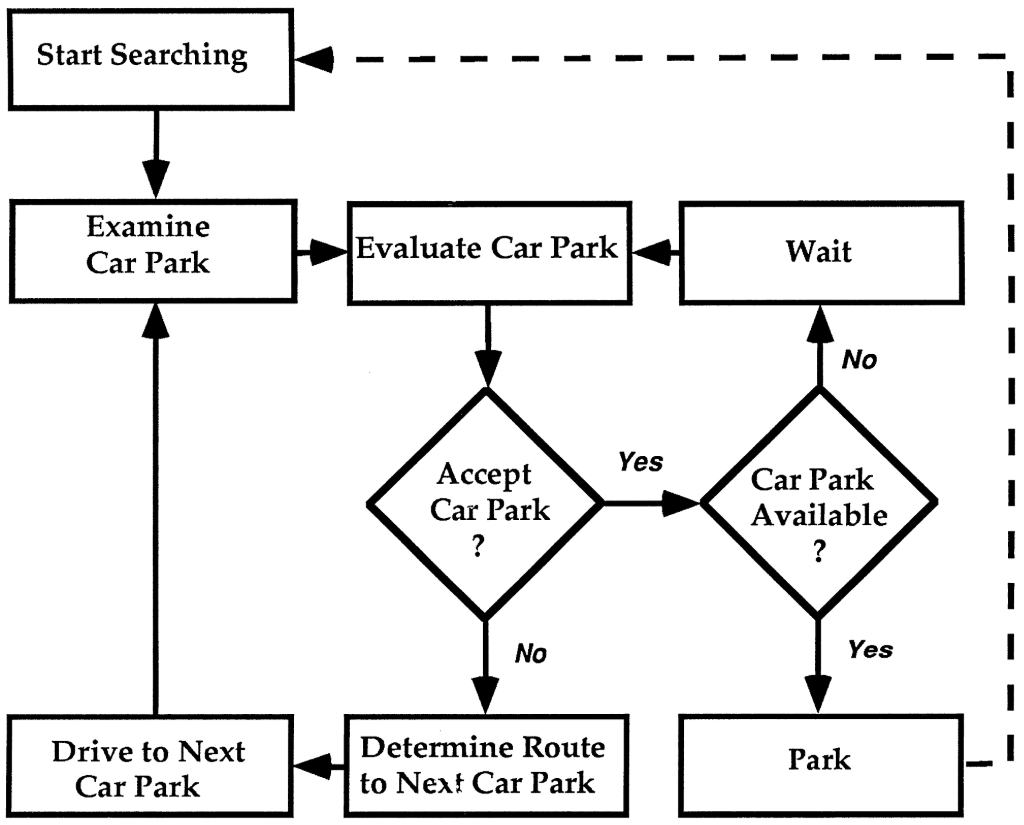
\includegraphics[width=.75\textwidth]{images/thesis_parking_search_process_thompson1998.PNG}
    \caption[Parking search process]{Defined by \citeauthor{Layzell1985} (\citeyear{Layzell1985}) and \citeauthor{Polak1989} (\citeyear{Polak1989}), parking choice may be considered as a search process in which motorists make linked decisions based on updated knowledge gained from experience. Parking choice Figure adapted from \citeauthor{Thompson1998} (\citeyear{Thompson1998}).}%
    \label{fig:parking-process-thompson}%
\end{figure}

In \citeintext{Salonen2013}, the accessibility disparity is studied in a comprehensive manner. Many earlier accessibility studies are cast into doubt as they have been simplifying the subject matter, using methods that are not satisfactorily explained, or are simply incompatible. \citeauthor{Salonen2013} employ real data in finding compatible methods for calculating travel times for both private car and public transport. Introducing the \textit{door-to-door approach}, the researchers strove for maximum realism when calculating the duration of entire trips, or \textit{travel chains}. In the door-to-door approach for private car, all realistic parts of a journey is taken into account (figure~\ref{fig:door-to-door}). The trip starts at the point of origin (O), from where one walks to where their car is parked at (P). The car drive segment commences, and continues until the earliest place where one would like to park at. This is where the parking process starts (see figure~\ref{fig:parking-process-thompson}), and it continues until a parking place is found (O). Finally one walks to the final destination of their journey (D). The door-to-door approach for the private car draws attention to a severely understudied subject, the parking process at the end of every trip made. While they accurately demonstrated the events that take place in realistic private car trips, \citeauthor{Salonen2013} themselves touched the subject of parking process only fleetingly. Notably, a parking process comparable to the one included in the door-to-door approach is described and employed in literature as early as in the 1960s (the "park-and-visit" approach, \cite{Inwood1966}; \cite{May1985}; \cite{Belloche2015}). 

\begin{figure}[H]%
    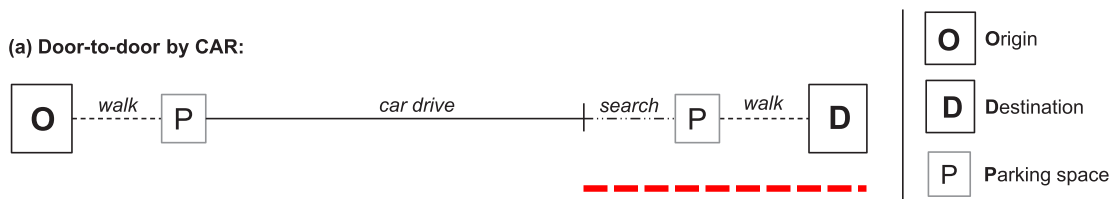
\includegraphics[width=\textwidth]{images/door2door.png}
    \caption[Door-to-door approach]{The entire travel chain of a private car using the door-to-door approach. The red dashed line represents the parking process segment of the travel chain. Figure adapted from \citeintext{Salonen2013}.}%
    \label{fig:door-to-door}%
\end{figure}

In this literary review to parking survey, it became apparent that most studies in this field employ a computational model to predict availability or use of parking spaces. Parking survey studies were sparse in number, and according to \citeintext{Diallo2015}, this is because the cost or difficulty to access appropriate data. They also note that complexity and extent of such studies work as a detriment.

In one computational model, \citeintext{VanDerGoot1982}, based on a parking study in the city of Haarlem, the Netherlands, showed that walking time strongly influenced drivers' choice of parking. An additional finding was that with the parking purpose of "shopping", longer walking times led to longer parking times, and shorter walking times translated to shorter parking times. In addition, in shopping trips, destination choice is influenced by the parking search time (\cite{Axhausen1993}). However, it is shown in literature that long term experience in parking search or knowledge of the area does not automatically result in better parking choices or make the parking search shorter (\cite{Thompson1998}; \cite{Teng2002}). \citeintext{Guo2013} has explored parking search process through an agent-based model in which a supply and demand are incorporated with sequential game-theoric capacity model to account for motorists' psychological attitudes in university campuses in the United States. 

\citeintext{Benenson2008} proposes a parking process model that is spatially explicit and agent-based (termed "PARKAGENT"). This means that the model takes urban elements essential for investigating parking process into account and gives agents instructions on how to react in different circumstances, such as reactions to lack of parking spaces and parking enforcement efforts, to simulate parking behaviour of motorists. This paper shows that the addition of a new parking facility does not much improve average parking search time and walking distance for on-street parking motorists. This was because the new facility, essentially, would change the supply and demand scenario of that area, bringing in motorists to the area who have their journey destinations further away. The paper also states that traditional parking modelling is insufficient in saturated parking situations (most major cities), as it is not possible for these models to consider actions of independent agents which can make decision on exact GIS data. A detailed view into "PARKAGENT" is described in \citeintext{Martens2010} alongside with a performance comparison to a non-spatial model of parking. A finding from this paper states that if parking turnover is low for a location (15 percent in an hour), the parking occupancy level of 85 percent, proposed by \citeintext{Shoup2004}, can be raised up to 95 percent. Parking occupancy level can be adjusted with changes to parking fees. The paper also states that if parking turnover reaches 50 percent for an hour, the aforementioned optimisation does not work.

Furthermore, in \citeintext{Levy2015} propose the model termed "PARKFIT", an GIS algorithm for estimating parking patterns without the need for in-situ behavioural data, and an continuation for the research carried out on "PARKAGENT". If high-resolution infrastructure GIS layers are available, the algorithm can be used to produce estimations -- map views -- about average distances between private cars aiming for a specific destination and the actual destination, and additionally the proportion of cars that fail to find a parking spot. The model, however, does not include parking search time. 

In a commendably open, data-driven study, \citeintext{Aryandoust2019} provide methodology and tools for modelling car parking density maps using only travel time measurements. In the study, the freely available Uber travel time data is used to generate maps for 34 cities in multiple countries. \citeauthor{Aryandoust2019} manage to reach 90 percent accuracy for parking densities and 93 percent for circadian rhythm of the traffic in the chosen city of validation, Melbourne, Australia.

% \cite{Harris1997}: evaluate parking space availability at university campus 
% \cite{Saltzman1997}: on-street parking issues
Simulation to evaluate parking space availability has also been utilised in, for example, \citeintext{Harris1997} and \citeintext{Saltzman1997}.

\newpage
\subsection{Parking time estimations}
\justify

In accessibility studies, the estimations and measurements for parking times are relatively scarce and a understudied subject. In Finland, a parking research was made for the city of Tampere (\cite{Kalenoja2003}). The authors interviewed individuals that had just finished parking, and were enquired after circumstances behind the parking, such as the factors that made them decide on the current parking place and from what direction they drove to the parking place location. In this study, 55 percent of interviewees had parked into a parking garage, 33 percent on-street and 13 percent in other areas. Over 60 percent of all interviewees reported that a short walking distance to their destination was of importance. The average time to find a parking place was 0.42 minutes on weekdays (table~\ref{tab:kalenoja-parktimes}).

\begin{hyphenrules}{nohyphenation}
    \begin{table}[H]
        \centering
        \caption[Parking time results in Kalenoja \& Häyrynen 2003]{The average time (minutes) to find a parking place in different types of locations in Tampere, Finland (\cite{Kalenoja2003}).} 
        \label{tab:kalenoja-parktimes}
        \begin{tabular}{ llll }
            \toprule
            Parking place type  & Weekday   & Saturday  & Overall \\
            \midrule
            On-street           & 0.73      & 2.08      & 0.80 \\
            Other areas         & 0.16      & 0.38      & 0.18 \\
            Parking garages     & 0.22      & 0.55      & 0.33 \\
            Overall             & 0.42      & 0.65      & 0.46 \\
            \bottomrule
        \end{tabular}
    \end{table}
\end{hyphenrules}

Internationally, \citeintext{Shoup2006} has been a landmark paper in private car parking time research. Mustering all research there was available on \textit{cruising for parking}, Shoup was able to display a compilation of results from a wide temporal and spatial pool. The gathered data showed that a range of 8--74 percent of a total trip was spent in cruising for parking. The average time to find a curbside parking place was in the range of 3.5--14 minutes. Shoup himself acknowledges the wide variance, saying that in reality some cities may have zero time spent in cruising for parking, while in other locations most of a journey made with private car consists of it. Regarding time spent in searching for parking when traveling by private car, \citeintext{Polak1990} states that it may constitute up to 25 percent of the average total travel time. According to \citeintext{Axhausen1991}, motorists valuate short parking search times over the driving time, with parking search time being up to two times more valuable. \citeintext{Parmar2020} suggest, based on their literature review, that motorists prefer to minimise the "out-vehicle" costs of parking charges, cruising for parking, and walking times, rather than the costs pertaining to the car itself, such as fuel cost and driving time.

In a parking time research carried out in France, it was found out that the average parking search time was especially severe in Paris. In the districts studied in Paris, parking search lasted on average 10 minutes in Commerce district and 7.7 minutes in Saint-Germain district. Extrapolating their results to the entire France, the researchers estimated that 70 million hours, each year, is spent searching for parking places (\cite{Gantelet2006}). In an other parking time focused paper, on-street parking was modelled and validated with a parking survey. The survey, conducted in Lyon, France, showed especially intolerable parking times in districts near the center of Lyon: an average searching time of 11.1 minutes for Part-Dieu, 9.6 minutes for Charpennes, and 6.3 minutes for Belges. All of these districts provided parking free of charge. In this study, the longest average parking search duration for a district with parking meters was the center of Lyon, Presqu'île, with a result of 6.2 minutes (\cite{Belloche2015}).

\newpage
\subsection{Research in parcipatory GIS and map surveys}
\justify

In \citeintext{Salonen2014}, participatory GIS (PPGIS) was employed in understanding what is the character of daily mobility in the Helsinki Capital Region and how often fastest travel mode is selected in these trips. The data received from respondents was used in conjunction with advanced travel time models based on real world GIS data such as the Digiroad dataset by Finnish Transport Infrastructure Agency. In this study, respondents most often chose non-optimal travel modes on "bounded trips" (work, school, or day care) and that many of the respondents are ready to choose a slower, and less carbon emission intensive means of travel.

\citeintext{Laatikainen2015} made use of PPGIS in the context of accessibility to urban aquatic environments and the environmental justice perspective that is included in a premise such as this. Employing "SoftGIS" methodology, the researchers were able to gather large amounts of data from users of urban environments through a easy-to-use user interface on the internet (\cite{Kytta2011}). The researchers had the opportunity to make use Finnish Population Register to select group of potential respondents representative of the study area, the Helsinki Capital Region. In some of the results, researchers point out that even though water is almost omnipresent in the Helsinki Capital Region, the utilisation of PPGIS revealed that proximity of a body of water does not have a clear influence on the real usage, or travel distances and times. This being said, the results showed that in many cases the body of water nearest to an individual was undesirable in some way, prompting the individuals to seek amenities along waterside further away. Also, while some areas of the Helsinki Capital Region are closer to more water, this fact did not automatically mean good access because of matters such as land ownership issues.
\import{content/}{c2_background.tex}%

% DATA AND METHODS
\newpage
%\section{Data and methods}
\subsection{General workflow}
\justify

A selection of web applications were designed and programmed for this thesis. In this chapter the process to create these applications is presented, from the design board to a functional web application to the end stage of data processing and visualisation. Four applications are presented in this chapter: a spatial web survey for data collection, and three separate web applications for the analysis and visualisation of the survey results.

Essential data for this research was provided by Statistics Finland, the research group Digital Geography Lab of University of Helsinki, the municipalities of Helsinki Capital Region, and Finnish Environment Institute. The research area of this thesis was based on PAAVO open data by postal code area (\cite{StatisticsFinland2019a}. Data such as the CORINE Land Cover 2018 artificial surface polygons and areas of urban structure were utilised to provide additional explanatory variables in the survey data (\textcolor{red}{cite corine}; \cite{Ristimaki2017}). For the visualisation of the survey results, various data by Statistics Finland was used (\cite{StatisticsFinland2012}).

Several programming languages were used to develop the survey web application and the subsequent data processing, analysis, and visualisation applications. The survey itself was created with HTML, JavaScript and PHP, with the essential help of Leaflet, a JavaScript mapping library (\cite{Agafonkin2019}). Data processing was a shared process between Python and R. Initial processing was done in Python and the analysis and visualisation in R. In Python, the library GeoPandas was in a central role, while interactive analysis and visualisation applications were created with the library Shiny (\cite{GeoPandasDevelopers2019}, \cite{Chang2019}). The thesis itself was written with LaTeX, a document preparation system, using the online LaTeX editor Overleaf (\textcolor{red}{cite}).

Initially, the research survey strove to collect parking event data on the precise temporal and spatial resolutions of an individual parking event and its exact coordinates, respectively. This first version of the survey created with Survey123 for ArcGIS was released to a small group of people before a planned larger roll-out, but it was quickly decided that a survey of a more general spatial and temporal resolution was needed to secure enough responses. After some consideration, one was programmed from the ground up using HTML and JavaScript. In this new survey, which was rolled out in May 2019, the respondent would send data about their parking activities in a specific postal code areas in a general sense, summing up their experiences in the most recent two years. The reduction in data resolution was substantial, but would still have more spatial fidelity than the existing parking time data in Helsinki Region Travel Time Matrix 2018 (\textcolor{red}{ttmcite}).

The survey was carried out in the four municipalities of Helsinki Capital Region. An invitation to participate in the survey was spread mostly in city district and neighborhood groups in Facebook. The response collection period continued until October 2019. The survey gathered, in total, 5222 responses from 4309 unique IP addresses.

After the conclusion of the data collection phase, the survey data was processed, analysed, and visualised using Python and R programming languages. The process started with anonymisation of the IP address data, and moved on to the processing proper. The objective of the data processing in Python was to bind the survey data with a selection of open spatial data in an effort to create additional explanatory variables for analysis.

The survey result analysis and visualisation was carried out in R. Utilising Shiny, a web application framework library for R, data analysis and visualisation applications were programmed for efficient and flexible data analysis for this thesis, but also to release the survey results to the public, maintaining the mission of openness and transparency of this thesis. \textcolor{red}{mieti josko avaisi shinyappien sisältöä tähän}

The general workflow of the thesis data processing can be viewed in figure~\ref{fig:gen_workflow}.

\begin{figure}[H]
    \centering
    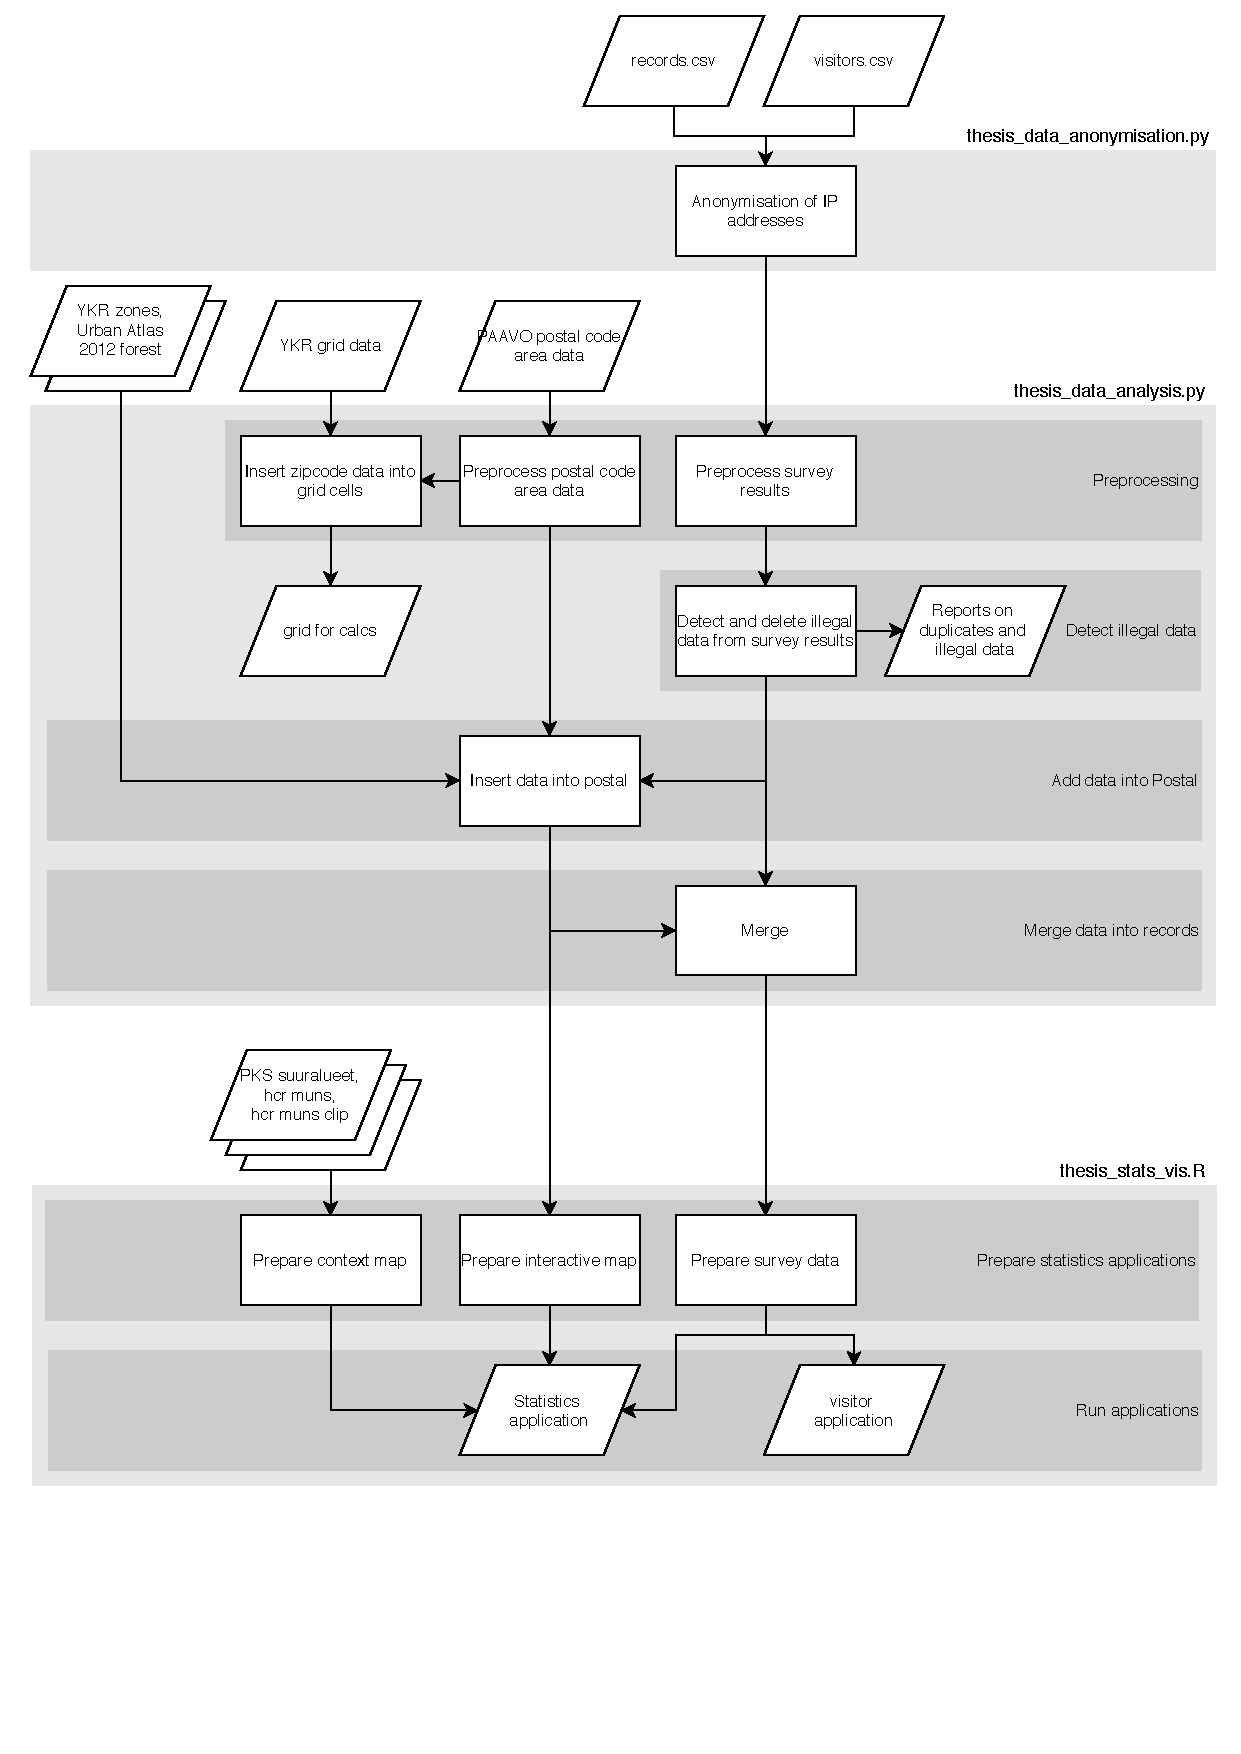
\includegraphics[trim=0.5cm 2.0cm 0.5cm 0.5cm,width=\columnwidth,scale=0.5]{thesis_workflow.pdf}
    \caption{The general workflow of the thesis survey data processing in Python and R.}
    \label{fig:gen_workflow}
\end{figure}
\pagebreak

\newpage
\subsection{Study area}
\justify
% https://www.hel.fi/hel2/Helsinginseutu/HS_tunnusluvut/liikennemaara_ja_autonomistus.pdf
% https://www.hsl.fi/sites/default/files/19_2016_auton_omistus_helsingin_seudulla.pdf
% https://www.hsl.fi/tutkimukset/muut-selvitykset
% http://pxnet2.stat.fi/PXWeb/pxweb/fi/StatFin/StatFin__lii__mkan/

\textcolor{red}{add content to this chapter} The study area of this thesis is the Helsinki Capital Region in Finland. It comprises of municipalities of Helsinki, Espoo, Vantaa and Kauniainen. The total population of the metropolitan area is 1.5 million \textcolor{red}{LÄHDE}. In practice, the whole area amalgamates as one complete functional area with boundaries of the municipalities indistinguishable at the street level. The Helsinki Capital Region faces increasing pressure to manage its traffic because \textcolor{red}{LÄHDE}. Of these four municipalities Helsinki is the hub, and considered to contain the only inner city features of the municipalities (\textcolor{red}{syke-urbanareas}). Espoo, Vantaa and Kauniainen mostly consists of suburban areas with occasional industrial areas and large shopping complexes placed throughout the area. The Helsinki Capital Region is served with a high-performance public transport system comprised of buses, train, subway, and tram in Helsinki. Recently, in 2017, the subway expanded from Helsinki to Espoo, triggering a new phase of quickly evolving cityscape in the surroundings of the new stations.

\begin{figure}[H]%
    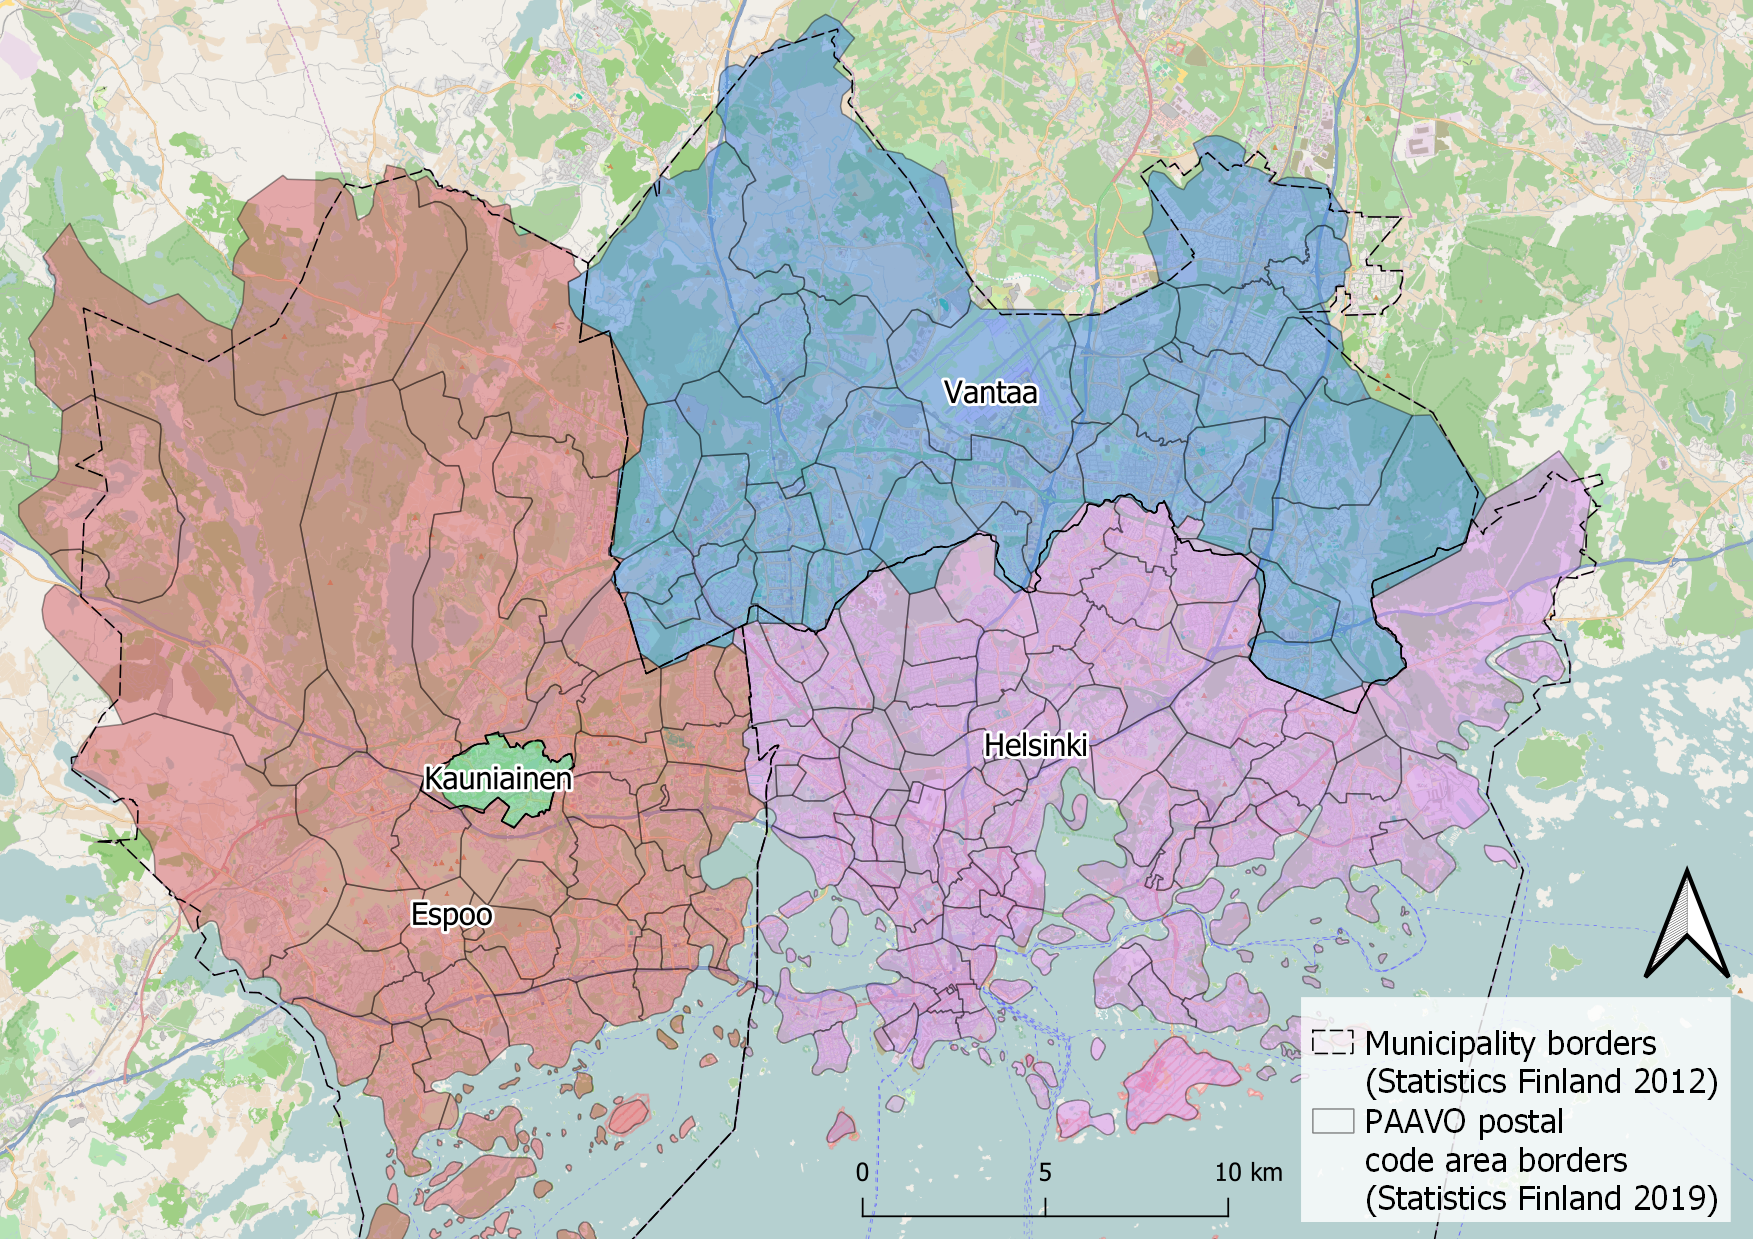
\includegraphics[width=\textwidth]{images/thesis_resarea.png}
    \caption[Research area map]{Map of the Helsinki Capital Region, the research area of this thesis. This research focuses on PAAVO postal code areas. The data has a municipality value for each postal code area (see the colouring of areas and map legend) but the areas do not completely align with the official municipality boundaries. \textcolor{red}{osmcite}}%
    \label{fig:thesis_resarea}%
\end{figure}

Despite the extensive service level of Helsinki Capital Region public transport, households especially in Espoo, Vantaa, and Kauniainen remain dependent on personal vehicles (\textcolor{red}{LÄHDE}). 

\newpage
\subsection{Data}
\justify

The foundation of this research is the dataset \textit{PAAVO -- open data by postal code area} (abbreviated \textit{postal} in this thesis) (figure~\ref{fig:paavo_resarea}). This data provides a large selection of data regarding the population of every postal code area in Finland. This includes detailed demographics and data about employment by field which follows the industrial classification TOL 2008 (\cite{Tilastokeskus2008}). However, this thesis only utilises the spatial definitions of the postal code areas, using these polygons to differentiate areas from each other in the web survey. This research makes use of the PAAVO 2018 dataset, released in January 2019.

In this thesis, the \textit{CORINE Land Cover 2018} (abbreviated \textit{CORINE}, figure~\ref{fig:datalayers}) vector format dataset is used to locate built area, or artificial surface, in the Helsinki Capital Region (\textcolor{red}{corinecite}). Provided by Finnish Environment Institute, CORINE contains polygonal data about land cover and land use for the entire nation in different hierarchy levels. In this thesis, the hierarchy level 1 value \textit{Artificial surfaces} is used. The minimum unit depicted in this dataset is 25 hectares in area or 100 meters in width. This slightly coarse data fits well with the spatially simplified nature of PAAVO postal code areas. CORINE dataset is an integration of automated satellite image interpretation and existing digital map data. \textcolor{red}{lisää taulukko siitä mitä level 1 artificial surfaces sisältää}

A main focus in this thesis was to compare the thesis survey results with \textit{Helsinki Region Travel Time Matrix 2018} (abbreviated \textit{TTM}), a dataset provided by Digital Geography Lab, a research group based in the University of Helsinki, the department of geosciences and geography (\cite{Tenkanen2018}). Their newest dataset provides travel times for public transport, private car, walking, and bicycling between all MetropAccess-YKR-grid cells (n=13231) \textcolor{red}{varmista että selitetty tätä ennen metropaccess ykr}. All travel times in this dataset were calculated using the door-to-door approach, which incorporates all parts of a journey from place A to place B into the travel time, including walking from one's home door to the car or bus stop and the time spent searching for parking. This thesis focuses on journeys made by private car.

\textit{MetropAccess-YKR-grid} (abbreviated \textit{grid}, figure~\ref{fig:datalayers}) is a spatial dataset consisting of cells with the dimensions of 250 by 250 meters (\cite{Toivonen2014a}). The dataset is used in the MetropAccess project of Digital Geography Lab and is based on the YKR data provided by Finnish Environment Institute and Statistics Finland (\cite{StatisticsFinland2020}). \textit{Grid} is a simple dataset and contains the spatial coordinates of cells and their identifiers, called the YKR ID. Using the YKR ID it is easy to connect \textit{TTM} data with the statistical data provided by Statistics Finland, allowing wide-ranging possibilities for further research.

All postal code areas in the survey results were classified with the \textit{zones of urban structures} (officially \textit{Yhdyskuntarakenteen vyöhykkeet}, abbreviated \textit{YKR zones}, figure~\ref{fig:datalayers}) (\cite{Ristimaki2017}). Utilising the same statistical grid of 250 x 250 meters as MetropAccess-YKR-grid, \textit{YKR zones} classifies grid cells to produce pedestrian, public transport, and automobile zones in and around Finland's urban regions using the theory of urban fabrics. According to this theory, these three zones developed during different times in the urban region's history (\cite{Newman2016}). In this thesis, every postal code area is assigned with a class defined in the \textit{YKR zones} based on which class has the largest presence. Adding this data into the survey results aimed to provide more possibilities to explain the hypothetical dissimilarity of survey results in different parts of the Helsinki Capital Region.

\textit{The regional division maps of Helsinki Capital Region} (officially \textit{Pääkaupunkiseudun aluejakokartat}, abbreviated \textit{subdivisions}, figure~\ref{fig:subdiv_placement}) was used in this thesis to analyse and visualise the survey results by subdivisions of Helsinki Capital Region (\cite{HelsinginEspoonVantaanjaKauniaistenmittausorganisaatiot2011}). Dividing the survey results into subdivisions would potentially give rise to local phenomena which would not be perceptible in the finest available level of spatial resolution, the postal code areas.

The dataset \textit{Regional population density 2012} (figure~\ref{fig:subdiv_placement}) was used in this thesis to visualise the boundaries of municipalities in Helsinki Capital Region (\cite{StatisticsFinland2012}). 

\begin{figure}[H]%
    \centering
    % use percentage of pagewidth with the syntax ".00\textwidth"
    \subfloat[CORINE Land Cover 2018 artificial surfaces in Kauniainen and eastern Espoo.]{{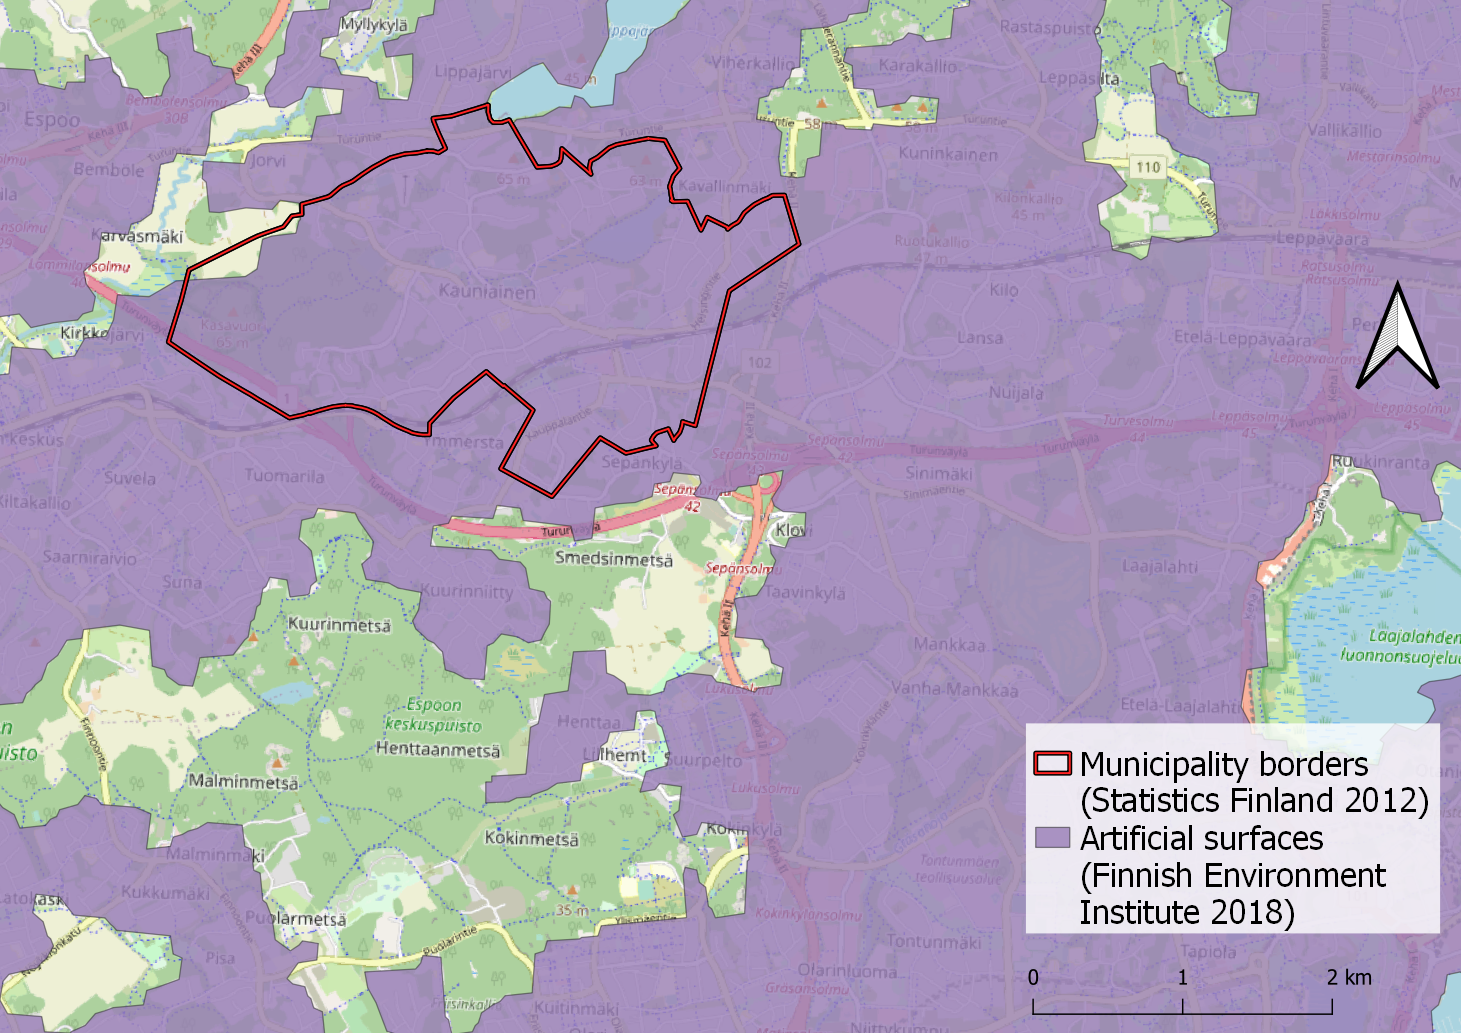
\includegraphics[width=.5\textwidth]{images/thesis_data_artificial.png} }}%
    \subfloat[Zones of urban structure in eastern Helsinki.]{{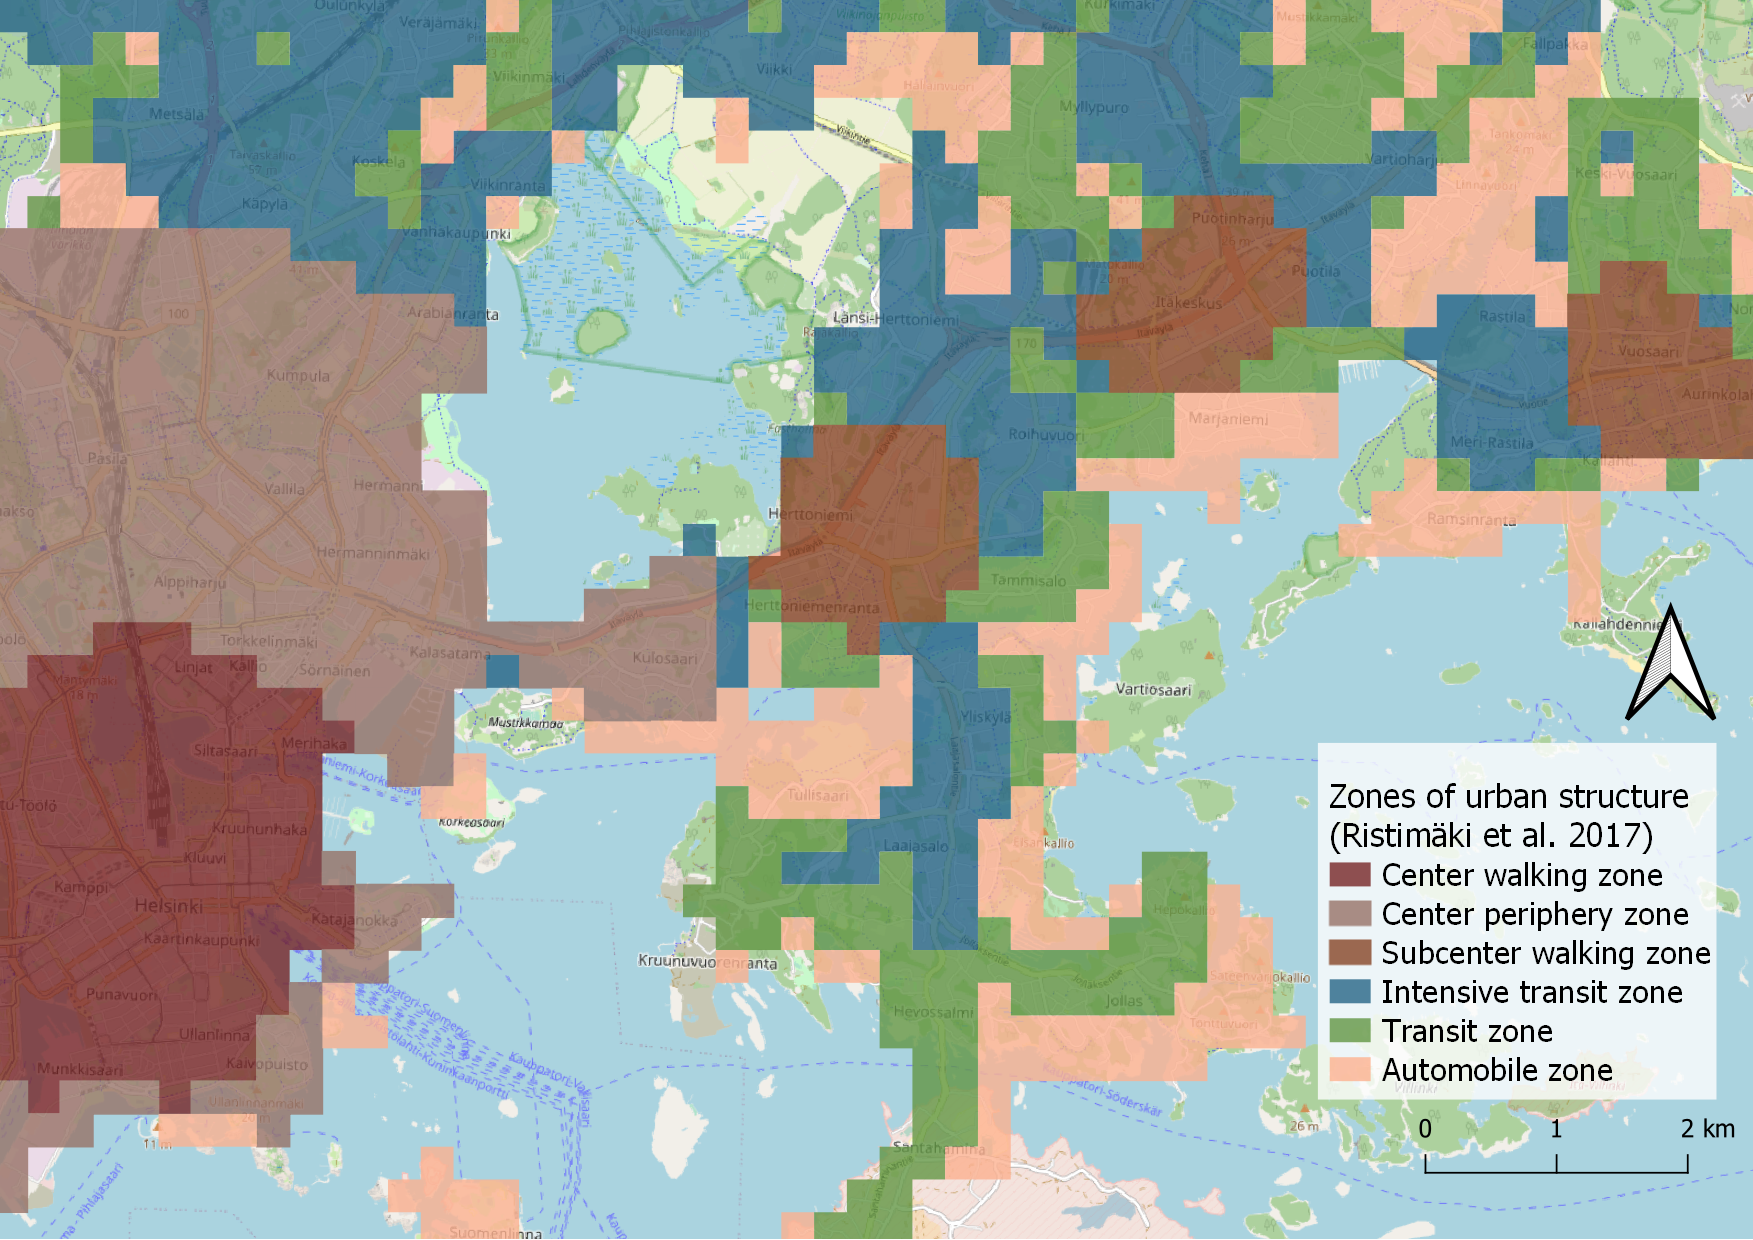
\includegraphics[width=.5\textwidth]{images/thesis_data_ykr_zones.png} }}%
    \quad
    \subfloat[MetropAccess-YKR-grid.]{{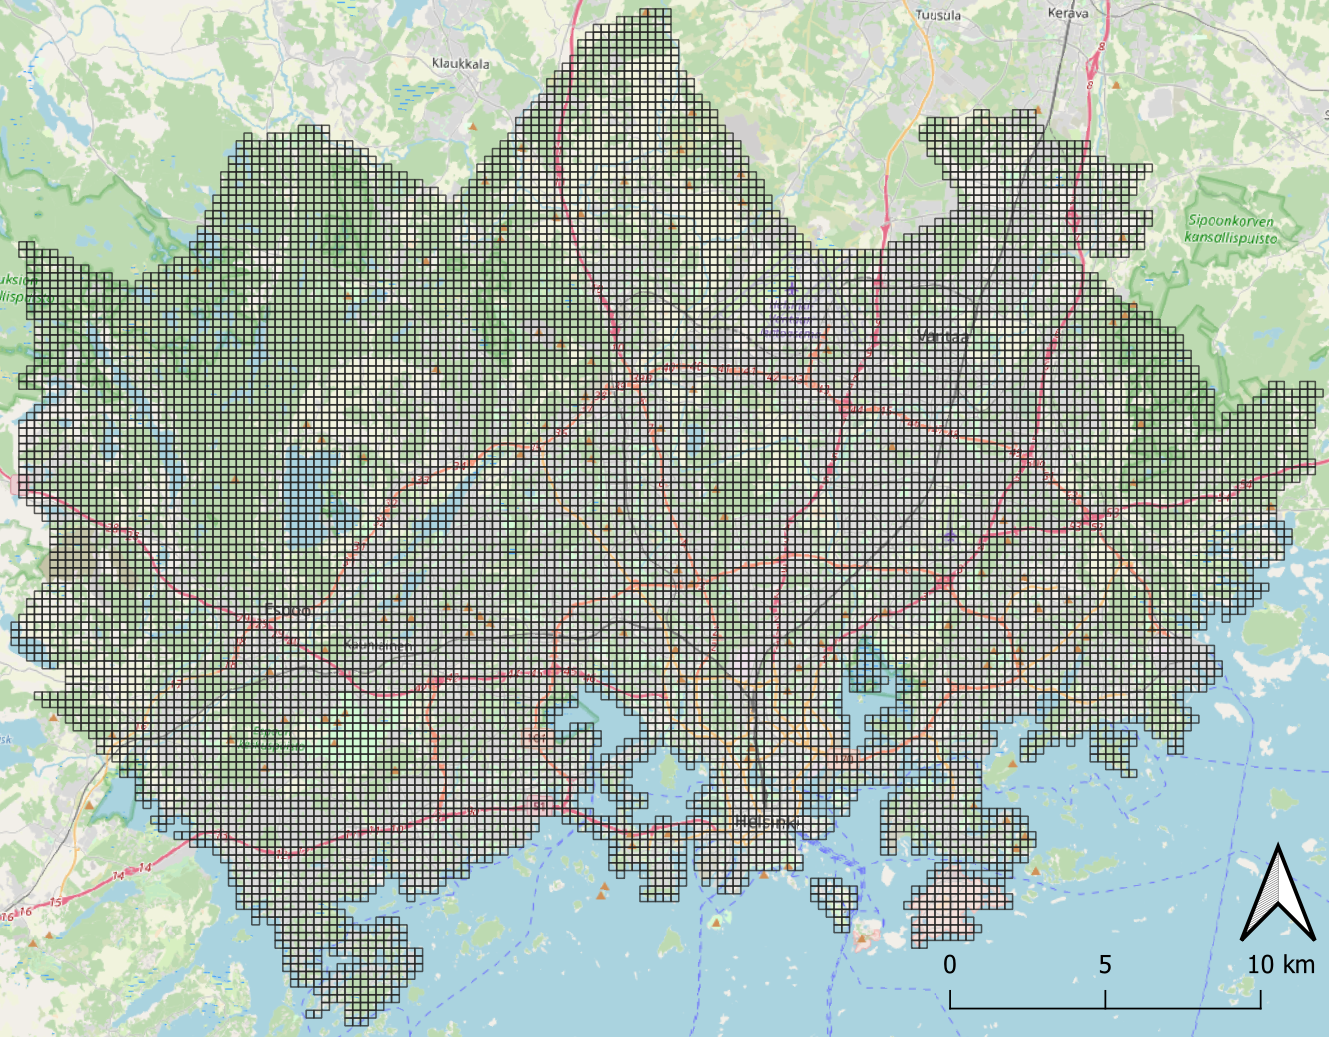
\includegraphics[width=\textwidth]{images/thesis_data_grid.png} }}%
    \caption[Spatial data]{Some of the spatial data used in the thesis. \textcolor{red}{osmcite}}%
    \label{fig:datalayers}%
\end{figure}

% hyphenrules: prevent hyphenation temporarily
\begin{hyphenrules}{nohyphenation}
    \begin{table}[H]
        \centering
        \caption[Thesis data]{Data utilised in the thesis.} 
        \label{tab:used_data}
        % use \scalebox{}{} to control table size. Note the additional curly brackets enveloping the entire tabular object
        \scalebox{0.8}
        % use \arraystretch to add whitespace between rows. \setlength\tabcolsep for columns
        {\def\arraystretch{1.5} 
        \setlength\tabcolsep{1.2ex}
        % One unit here is ">{\raggedright\arraybackslash}p{4cm}". \raggedright prevents justification of text and conveniently allows flush right or flush left, which is not possible with column command p{4cm} alone.
        \begin{tabular}{ @{} >{\raggedright\arraybackslash}p{4cm} >{\raggedright\arraybackslash}p{4cm} >{\raggedright\arraybackslash}p{4.5cm} >{\raggedright\arraybackslash}p{3.5cm} >{\raggedleft\arraybackslash}p{3.5cm} @{} }
            \toprule
            Data & Description & Purpose in thesis & Abbreviation in thesis & Citation \\
            \midrule
            CORINE land cover 2018 & Land use and land cover data in vector format & Artificial surface data & \textit{CORINE} & \textcolor{red}{cite} \\
            Helsinki Region Travel Time Matrix 2018 & Travel time and distance information for routes between all \textit{grid} cell centroids in the Capital Region of Helsinki & Use in travel time comparison calculations between \textit{TTM} and thesis survey results & \textit{TTM} & \cite{Tenkanen2018} \\
            MetropAccess-YKR-grid & Statistical grid of 250 x 250 meter cells for monitoring urban structure, Helsinki Capital Region area & Use in travel time comparison calculations between Travel Time Matrix 2018 and thesis survey results & \textit{grid} & \cite{Toivonen2014a}, \cite{StatisticsFinland2020} \\
            Paavo -- Open data by postal code area 2018 & Helsinki Capital Region postal code areas & Thesis research area and the basic unit of spatial resolution in the survey & \textit{postal} & \cite{StatisticsFinland2019a} \\
            Regional population density 2012 & Population density with municipality boundaries & Visualisation in R & \textit{hcr\_muns} & \cite{StatisticsFinland2012} \\
            Subdivisions of Helsinki Capital Region & The subdivisions of the municipalities of Helsinki Capital Region & Visualisation in R & \textit{subdivisions} & \cite{HelsinginEspoonVantaanjaKauniaistenmittausorganisaatiot2011} \\
            Zones of urban structure (Yhdyskuntarakenteen vyöhykkeet) 2017 & Delineation of urban areas based on the theory of urban fabrics & Data on spatial structure of urban areas & \textit{YKR zones} & \cite{Ristimaki2017} \\
            \bottomrule
        \end{tabular}}
    \end{table} 
\end{hyphenrules}

\newpage
\subsection{Used software}
\justify

A wide variety of software was used in the research for this thesis. The research strived for maximum openness and transparency and therefore much of the software employed in this work is free, open-source, or both. The research survey application utilised several essential web technologies such as JavaScript, HTML, CSS and PHP (table~\ref{tab:used_langs}). Using the web mapping library Leaflet, with the assistance of jQuery and other libraries, a modern and easy-to-use survey web application was created. Server-side, the programming language PHP was used to verify received data.

Data processing was carried out in Python 3.7.6 and R for Windows 3.6.3, with the initial processing done in Python and most of the analysis and visualisation in R (table~\ref{tab:used_langs}). Much of the work depended on additional software libraries available for the programming languages (table~\ref{tab:used_soft}). Python Anaconda version 2020.02 -- a distribution for Python for statistical computing -- provides the majority of the needed software libraries in the installation package, with the notable exception of GeoPandas, a library for geospatial pandas DataFrames in Python, and Shapely, a library for manipulation and analysis of planar geometric objects. In R, many libraries were used to achieve a comprehensive set of descriptive statistics. Libraries such as Shiny, ggplot2, and ggiraph formed the basis of the visualisation of the survey results.

% latex is not a programming language for the most part: https://www.quora.com/Is-LaTeX-a-programming-language
The thesis was written and typeset with LaTeX using the online LaTeX editor Overleaf. LaTeX is a document preparation system, used to create documents such as scientific articles. LaTeX adheres to the WYSIWYM (what you see is what you mean) system, as opposed to the "what you see is what you get" (WYSIWYG) system of text editors such as Microsoft Word, meaning that after establishing a set of parameters LaTeX will automatically compute the document formatting, while the user can concentrate on the document content. While LaTeX can be considered a programming language, it is more closely related to markup languages such as HTML (\textcolor{red}{cite}). In this LaTeX document, the LaTeX distribution TeX Live 2019 was used. Overleaf supports GitHub integration and as a result the complete thesis is available for viewing in the GitHub repository \textcolor{blue}{\url{https://github.com/sampoves/Masters-2020}} alongside with its entire development history. Additionally, the template of this thesis is provided at \textcolor{blue}{githublink, repo not started}.

In addition to the aforementioned technologies, the flowcharts in this thesis were created with the web application diagrams.net (\textcolor{red}{cite}). Most of the map visualisations of this thesis were made using the geographic information system application QGIS version 3.12.2.

% Consider! Removing \raggedright and hyphenrules will enable nice even table cells. Could be worth it to look into
\begin{hyphenrules}{nohyphenation}
    \begin{table}[H]
        \centering
        \caption[Thesis programming languages]{Programming languages, essential technologies, and \glspl{ide} utilised in the thesis, grouped by the function in this thesis.} 
        \label{tab:used_langs}
        \def\arraystretch{1.4}
        \setlength\tabcolsep{1.2ex}
        \begin{tabular}{ @{} >{\raggedright\arraybackslash}p{3cm} >{\raggedright\arraybackslash}p{4.5cm} >{\raggedright\arraybackslash}p{3.5cm} >{\raggedleft\arraybackslash}p{3.5cm} @{} }
            \toprule
            Programming language and \gls{ide} & Description & Purpose in thesis & Citation \\
            \midrule
            JavaScript, HTML, CSS (NetBeans 8.2.0) & Essential web technologies & Research survey programming, analysis and visualisation application programming & \cite{WHATWG2020}, \cite{W3C2020}, \cite{ECMA2019}, \cite{ApacheSoftwareFoundation2016} \\
            Python 3.7.6, Anaconda 2020.02 (Spyder 4.0.1) & Anaconda is a Python distribution for scientific computing & Survey data processing & \cite{Python3Reference}, \cite{AnacondaInc.2020}, \cite{SpyderProjectContributors2020} \\
            R for Windows 3.6.3 (RStudio 1.2.5033) & Programming language environment for statistical computing & Survey data analysis and visualisation & \cite{RCoreTeam2020}, \cite{RStudioTeam2015} \\
            LaTeX (Overleaf) & Document preparation system & Thesis formatting, structure, and writing & \textcolor{red}{latexcite, overleafcite} \\
            \bottomrule
        \end{tabular}
    \end{table} 
\end{hyphenrules}

\begin{hyphenrules}{nohyphenation}
    \begin{table}[H]
        \centering
        \caption[Essential software packages in thesis]{Essential software libraries used in the thesis. The complete list of libraries can be viewed in \textcolor{red}{appendix number something}.} 
        \label{tab:used_soft}
        \def\arraystretch{1.2}
        \setlength\tabcolsep{1.2ex}
        \begin{tabular}{ @{} >{\raggedright\arraybackslash}p{2.5cm} >{\raggedright\arraybackslash}p{3cm} >{\raggedright\arraybackslash}p{4cm} >{\raggedleft\arraybackslash}p{3cm} @{} }
            \toprule
            Programming language & Software package & Description & Citation \\
            \midrule
            % NB, manual positioning of the multirow label
            \multirow{3}{*}[-5ex]{JavaScript} & Leaflet 1.4.0 & Web mapping library for the research survey & \cite{Agafonkin2019} \\
            & jQuery 3.4.1 & Simplification of HTML DOM traversal and other features & \textcolor{red}{cite} \\
            & Font Awesome 5.13.0 & Font and icon collection & \textcolor{red}{cite} \\
            \greyrule
            \multirow{4}{*}[-6.5ex]{Python} & pandas 1.0.1 & Data analysis and manipulation & \cite{McKinney2011a} \\
            & GeoPandas 0.5.0 & Geographic data operations & \cite{GeoPandasDevelopers2019} \\
            & Shapely 1.6.4.post1 & Geometric objects, predicates, and operations & \cite{Gillies2019} \\
            & rtree 0.8.3 & Spatial indexing & \cite{Gillies2014} \\
            \greyrule
            \multirow{4}{*}[-7.0ex]{R} & Shiny 1.4.0.2 & Web application framework for R & \cite{Chang2019} \\
            & ggplot2 3.3.0 & Data visualisation & \cite{Wickham2016} \\
            & ggiraph 0.7.0 & Interactive ggplot2 graphics & \cite{Gohel2019} \\
            & dygraphs 1.1.1.6 & Interactive time series charting & \cite{Vanderkam2018} \\
            & fst 0.9.2 & High-performance writing and loading of data & \textcolor{red}{cite} \\
            \bottomrule
        \end{tabular}
    \end{table} 
\end{hyphenrules}

\newpage
\subsection{Methods}
\subsubsection{Considering survey development options}
\justify

To collect the areal parking data, the study required an interactive survey which respondents could use to submit their parking habits in a spatial fashion. To attract a largest possible number of submissions, the survey also needed to be of modern design, easy to use and its purpose easy to understand. The survey would have to be clear-cut, effortless to internalise and short in length as to prevent users getting frustrated and leaving before submitting answers. Design-wise, the spatial resolution of the survey was in question. The particular concern was that in the case of insufficient amount of answers, what kind of area delineation would be at the same time detailed enough but also streamlined enough to realistically reach results of good quality? This chapter strives to describe the process that would lead to the implemented web survey to accentuate the challenges this kind of research entail.

Once the consideration into options to produce the survey for this study had started, it quickly became apparent that there were few alternatives available and even fewer free, sufficiently customisable alternatives. Out of the proprietary options, Maptionnaire by the Finnish company Mapita was considered. They offer tailored map survey products with discounts for students. In return for the fee, a subscriber receives a time window in which to carry out their survey accompanied with tailored features and customer support -- the extent of features and support is determined by the price plan. The offered price was considered too steep for the thesis and Maptionnaire was passed on. 

Next Survey123 for ArcGIS was evaluated. An Esri operated service, Survey123 is used to create and analyse form based surveys (\cite{Esri}). It is included in the contract between University of Helsinki and Esri and thus was free to use for the study. One can quickly design a survey at the Survey123 website and share it immediately to respondents. Alternatively, the service is available as a desktop client, the Survey123 Connect, where Survey123 offers a wider range of possibilities for customisation with its adherence to the XLSForm standard. XLSForm is a standard to make authoring forms in Excel easier. With the customisability of XLSForm, users can design Survey123 surveys to the dot while employing the support for Excel style scripting for complex survey behaviour (figure~\ref{fig:survey123_xlsform}). Furthermore, Survey123 provides online tools for collaboration, analysis, and data viewing with many options for exporting the collected data.

\begin{figure}[H]%
    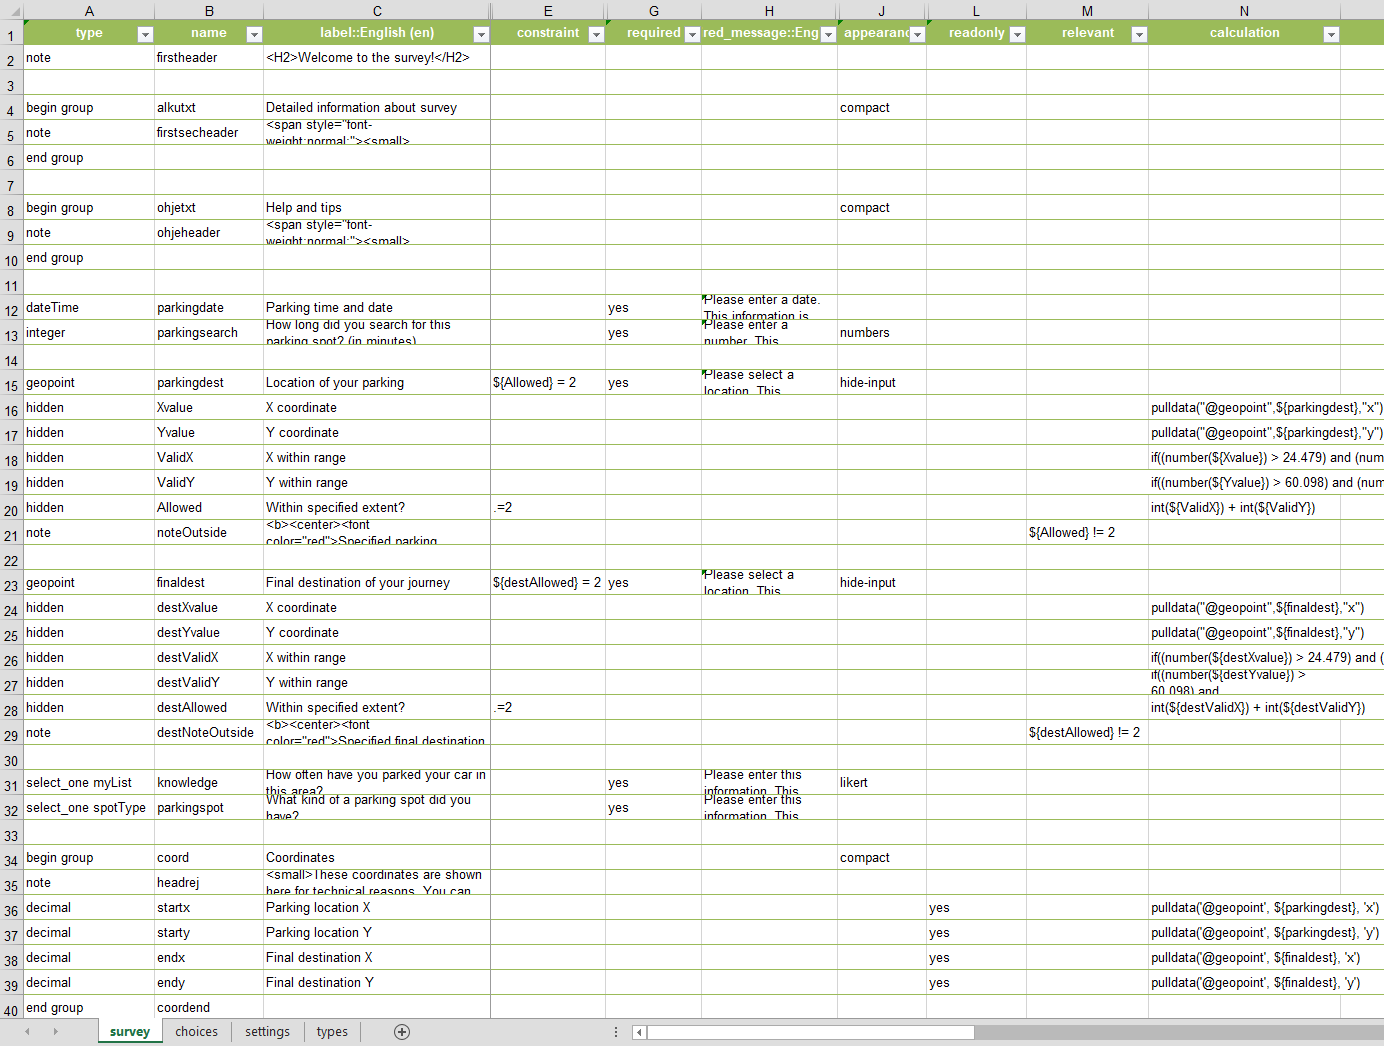
\includegraphics[width=\textwidth]{images/survey123_xlsform.png}
    \caption[Survey123 XLSForm view]{Survey123 XLSForm view in Microsoft Excel. Some parameter columns here are hidden to provide a view to the essential inner workings of the Survey123 form.}%
    \label{fig:survey123_xlsform}%
\end{figure}

% \ref{}: tilde (~) indicates a non-breaking space
In January 2019, the parking survey developed with Survey123 was deployed to friends and family, with a large scale marketing push on social media platforms planned for later. At its core, this survey asked respondents for specific parking events in Helsinki Capital Region they had had (figure~\ref{fig:survey123}). Respondents would pick an exact location on a map view for the location of their parked car and separately on a second map view the location of their final destination. In addition, respondents would fill the date and time of this parking event, how long it took for them to find a parking spot, how often they had parked to that area, and what kind of a parking spot they had taken. Respondents were asked repeat this process as many times as they had the will to do so.

The Survey123 survey was designed to reach the same spatial resolution as Travel Time Matrix 2018 with its MetropAccess-YKR-grid (grid cell 250 x 250 meters). Using exact coordinates of parkings and final destinations, it would have been possible to allocate each event to possibly two different MetropAccess-YKR-grid cell codes, reaching excellent spatial resolution. As MetropAccess-YKR-grid contains 13 231 grid cells, there was not enough resources for this master's thesis research survey to accumulate events for every grid cell, or even for most grid cells. If the data gathering campaign would have ended with insufficient amount of parking events, the backup plan was to employ an interpolation algorithm to generate approximate boundaries for the hypothetically varying parking times in Helsinki Capital Region. It was also considered that the exact coordinates of the parking events could be generalised to other boundaries, such as administrative areas like municipality subdivisions or postal code areas \textcolor{red}{explain why this was not done}. 

% utilises package subfig
\begin{figure}[H]%
    \centering
    \subfloat[Survey introduction and the date and time for the parking event.]{{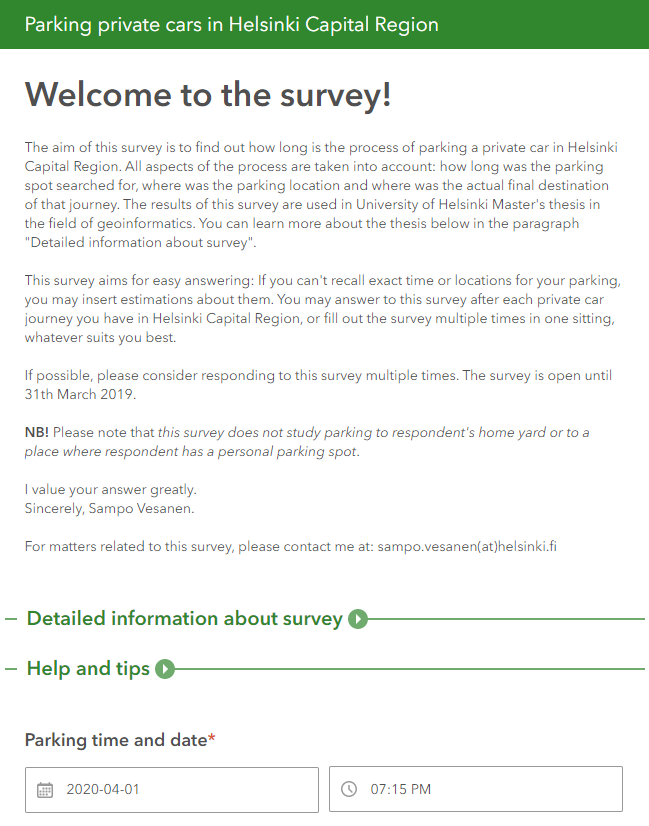
\includegraphics[width=5.5cm]{survey123_1.png} }}%
    \subfloat[Map panels for the parking location and the final destination.]{{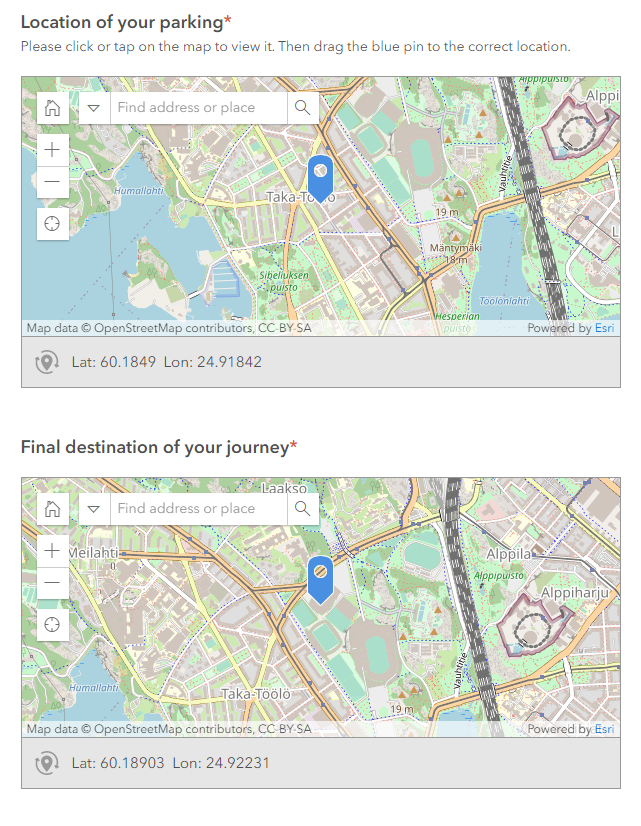
\includegraphics[width=5.5cm]{survey123_2.png} }}%
    \subfloat[Final questions of the survey.]{{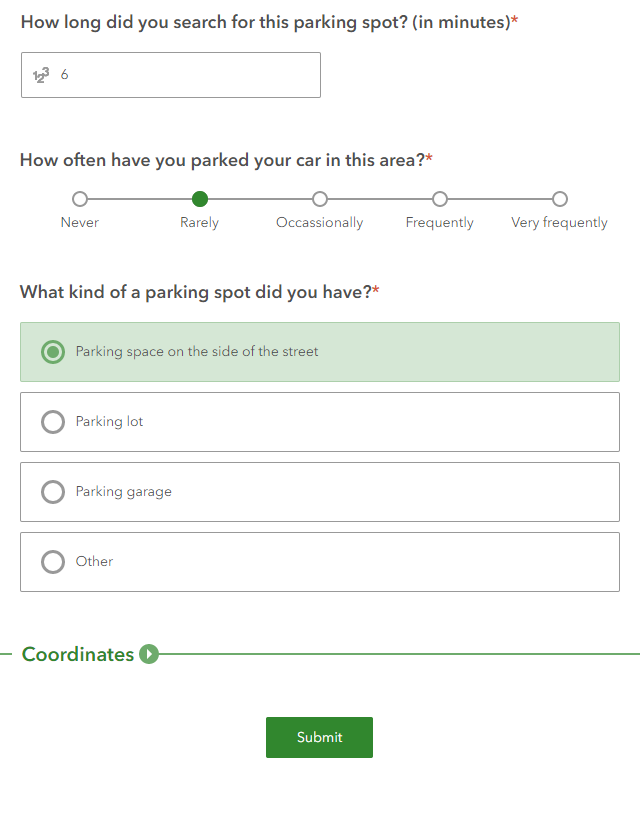
\includegraphics[width=5.5cm]{survey123_3.png} }}%
    \caption[The unused parking survey created with Survey123]{An example parking event entered into the parking research survey made with Survey123 Connect.}%
    \label{fig:survey123}%
\end{figure}

The survey was released even after Survey123 had proved itself unwieldly for the purposes of this research. The software was difficult to use because of an assortment of inconvenient design choices, unfinished functionality and a helping of software bugs. It was not possible, for example, to have respondents enter multiple parking events at once in a full screen map view. They would have to create a single parking event, send it, and then reload the survey to start from the beginning -- something a majority of prospective respondents would not have the patience for. Survey123 Connect version available at the time, 3.1.126, did not allow customisation of the post-submission message and therefore it would not be possible to efficiently direct respondents back to the form. In addition, recording coordinates from two map views was only possible through a bypass. The coordinates of the final destination would have to be printed on the form (hence the section "Coordinates" on the form in figure~\ref{fig:survey123}) and then these second set of coordinates could be saved into the survey data table in string format. The technical limitations of Survey123 as a spatial survey was witnessed also in the fact that it was not possible to add custom polygons on top of the map views. It was therefore impossible to delineate the research area for the respondents and accurately detect attempts to add parking events outside of Helsinki Capital Region.

The functionality of the released form was not reliable on the most popular web browsers such as Google Chrome and Apple Safari. Survey123 supported multi-language strings but it proved problematic to ensure that the form would open in the system language of most respondents, Finnish. In addition to this, the field for entering the specific time for the parking event was restricted to the 12 hour clock preferred in the US -- a system my target group would frown upon. To make matters worse, at that time there was a long persisting bug in Survey123 which produced unexpected behaviour, in some cases, with the use of "constraint", the parameter that controls which entered values are deemed illegal and which are not (\cite{GeoNet-TheEsriCommunity2018}). If any type of constraint statement was added, the finalised form would always claim that the related question input was invalid. The parameter would have to be left empty and therefore it was not possible to automatically prevent insertion of parking events happening in the future and excessively long times for searching for parking, reducing the quality of the survey data and making the survey form more confusing for the respondent.

\begin{figure}[H]%
    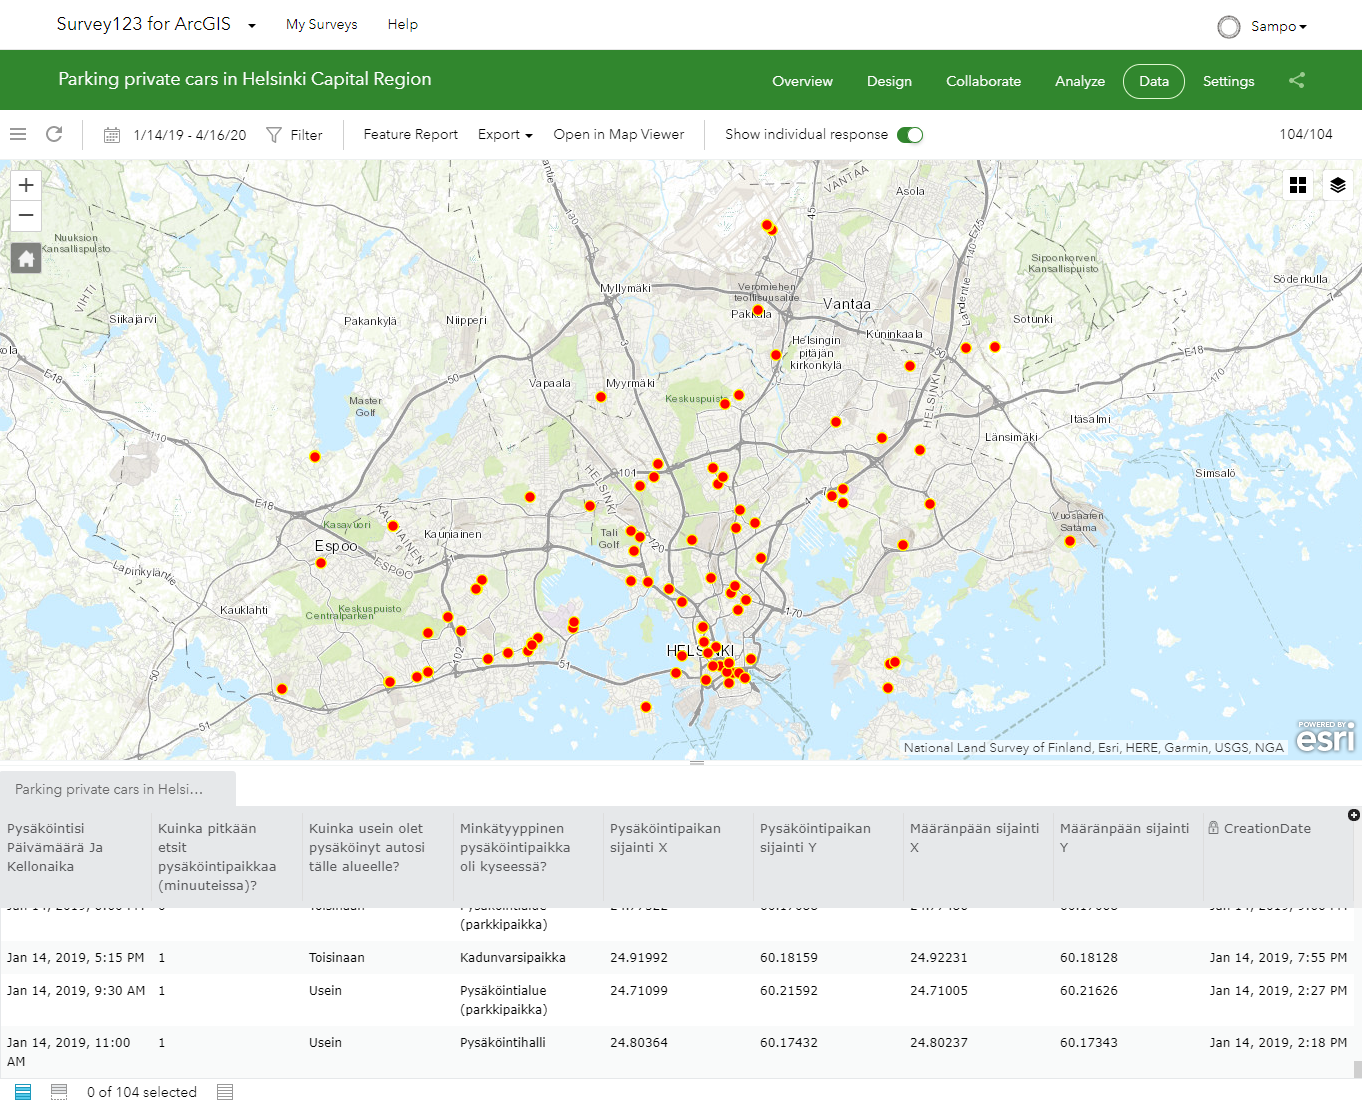
\includegraphics[width=\textwidth]{images/survey123_dataview.png}
    \caption[Survey123 data tab]{Survey123 for ArcGIS, "data" tab view in the application website. The research survey made with Survey123 received in total 104 parking events. The red dots are the final destinations of each parking event.}%
    \label{fig:survey123_dataview}%
\end{figure}

Despite the many technical incertainties of Survey123, the survey gathered more than one hundred parking events in one month (figure~\ref{fig:survey123_dataview}). This amount was achieved for the most part without advertising. Soon after the publication of the Survey123 parking survey it was decided, however, that the required spatial resolution for this research would need to be lower than exact points in an attempt to gather more responses from the entire research area. An additional deciding factor was the fact that with Survey123 respondents could not send multiple parking events with one survey session, making the form unwieldy and outdated in its rigid structure. It was argued that a more general scale would still be accurate enough to provide good data and a more generalised scale would make the survey easier to answer to and a more pleasant experience for the respondent. Postal code areas were deemed an acceptable compromise in spatial accuracy.

After careful consideration, it was decided that the survey for this thesis would have to be programmed from the ground up.

\subsubsection{Programming the parking survey}
\justify
To achieve maximum transparency and repeatability for this research, in addition to freedom in survey content and appearance, a survey web application was programmed from the ground up utilising HTML, JavaScript and PHP. The survey and its supporting infrastructure was installed on a virtual machine in CSC's -- the state owned ICT solutions company -- Taito supercluster. CSC offers virtual machines in several different hardware configurations, or flavors. The virtual machine flavor picked for this survey was \textit{standard.medium}, a flavor with 3.9 \gls{GB} \gls{RAM}, three virtual \gls{CPU}s and 80 GB of disk space. Running on the Linux distribution Ubuntu version 16.04, the backbone of the survey ecosystem was a LAMP stack, a software bundle which incorporates the Linux operating system, Apache web server software, \gls{mysql} relational database management system and the PHP programming language environment for server-side scripting. The public component of the survey is the front-end, the only component of the survey system a respondent would interact with (figure~\ref{fig:js_survey_welcome}). One may use additional software in a LAMP stack for extended functionality or can replace some of the components with a wide array of alternatives. This thesis utilises the components described in the table~\ref{tab:survey_components}.

\begin{hyphenrules}{nohyphenation}
    \begin{table}[H]
        \centering
        \def\arraystretch{1.2}
        \setlength\tabcolsep{1.2ex}
        \caption{Survey web application components} 
        \label{tab:survey_components}
        \begin{tabular}{ @{} >{\raggedright\arraybackslash}p{3cm} >{\raggedright\arraybackslash}p{3cm} >{\raggedright\arraybackslash}p{5.5cm} @{} }
            \toprule
            Component & Version & Description \\
            \midrule
            Ubuntu & 16.04.6 & Linux distribution, operating system for the virtual machine \\
            Apache HTTP Server & 2.4.18-2ubuntu3.9 & Web server software, manage website requests and responses \\
            MySQL & 5.7.25-0ubuntu0.16.04.2 & Relational database management system, survey database operations \\
            PHP & 7.0.33-0ubuntu0.16.04.1 & Programming language, used for server side scripting \\
            Parking survey front-end & 16.5.2019 & Survey visible to user, graphical user interface \\        
            \bottomrule
        \end{tabular}
    \end{table}
\end{hyphenrules}

Setting up the virtual machine for the use of the survey was a process of a few stages. The LAMP stack was installed on the fresh virtual machine with the command \code{sudo apt install lamp-server\^}. After the successful installation the MySQL tables were formed and relevant users created. The last step before a fully functioning web server was using root access to give the survey components permission to access relevant system directories. The parking survey's GitHub repository (\textcolor{blue}{\url{https://github.com/sampoves/parking-in-helsinki-region}}) may be viewed for the full step-by-step install procedure used to set up the web server for this thesis.

\begin{figure}[H]%
    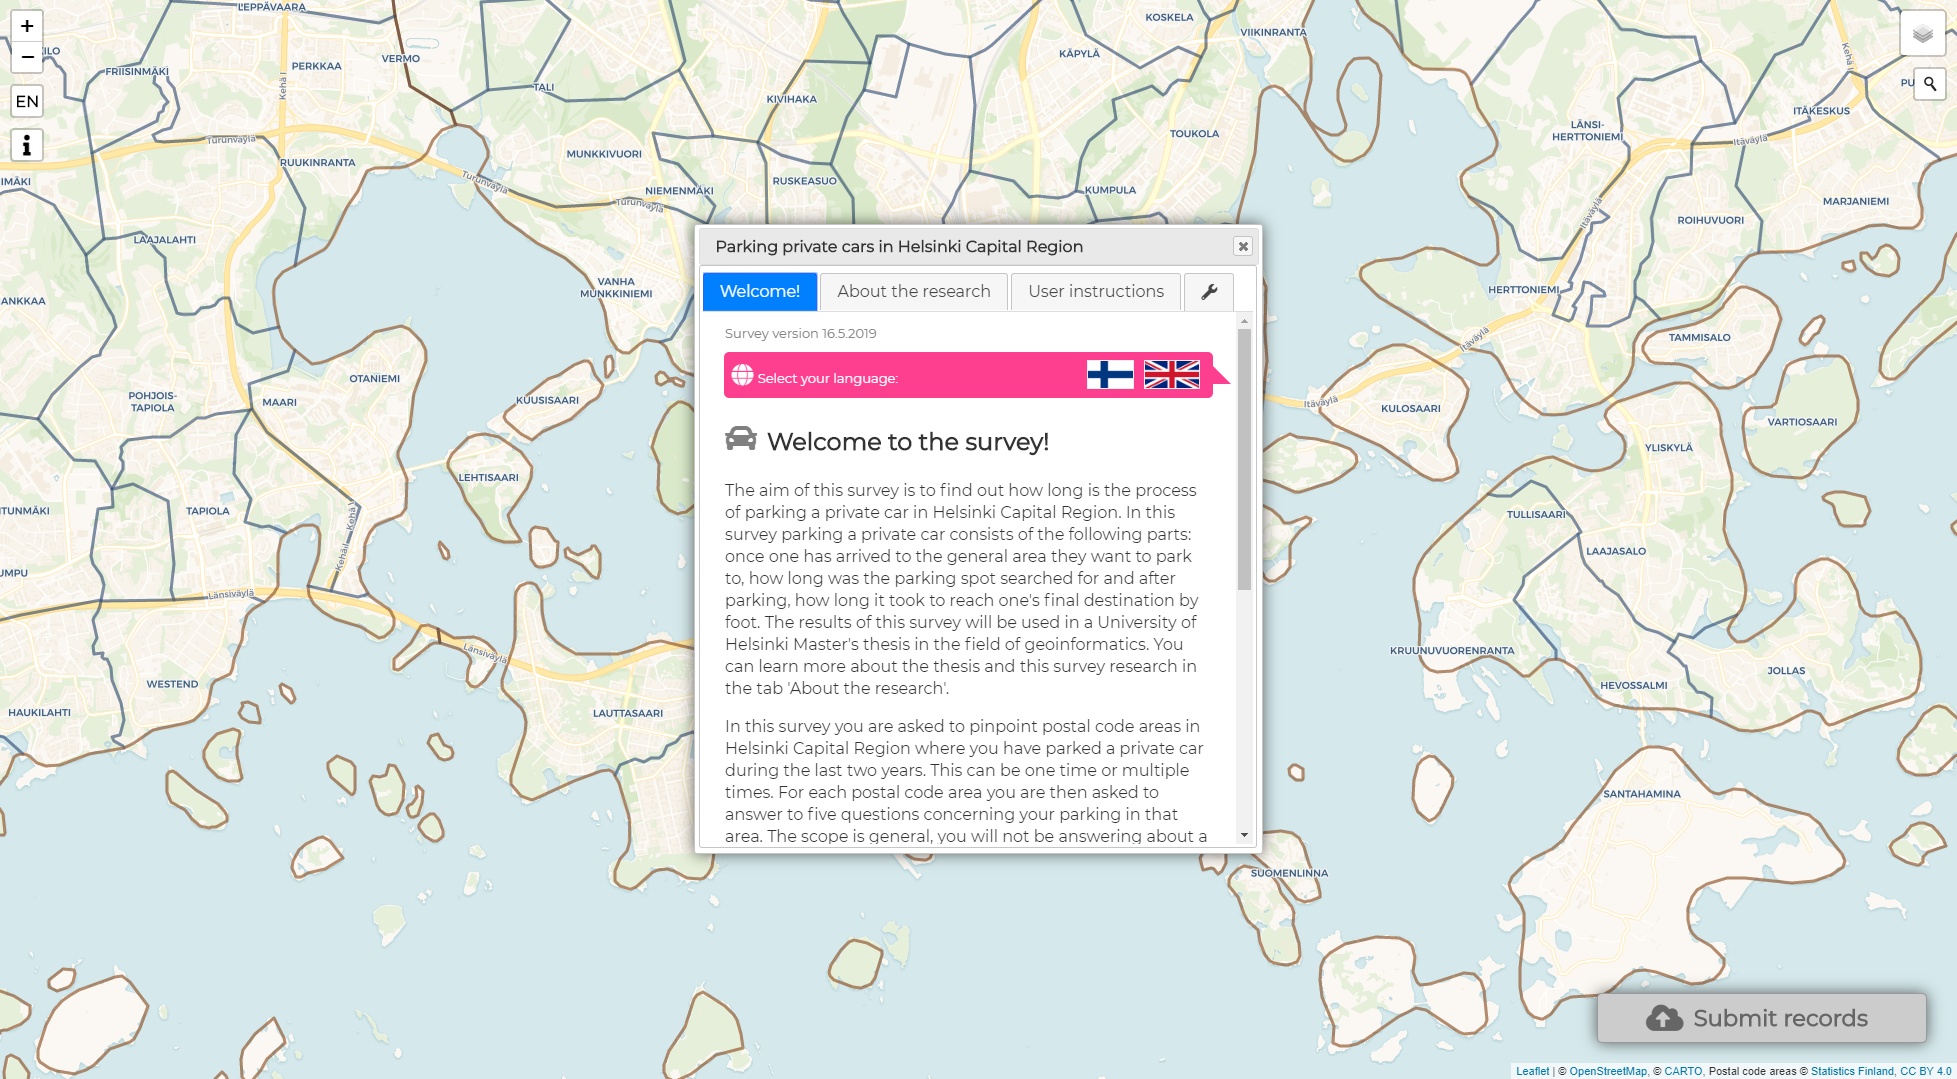
\includegraphics[width=\textwidth]{images/js_survey_welcome.png}
    \caption[Survey landing page]{The parking survey initial view with the welcoming dialog window.}%
    \label{fig:js_survey_welcome}%
\end{figure}

The survey front-end was programmed in NetBeans \gls{ide} 8.2 in mostly JavaScript using an open-source mapping library Leaflet (software version 1.4.0) in January--May 2019. In the survey, the respondent was presented with a map view of Helsinki Capital Region with its 167 postal code areas with the ability to drag the view, zoom in and out, search for places and addresses, choose the language between English and Finnish, and tweak various other settings to their liking. In this web survey, the respondent was asked to pick as many postal code areas as they could remember parking in in the last two years, and answer to five questions per each postal code area (table~\ref{tab:js_survey_questions} and figure~\ref{fig:js_survey_questions}). In each question, the respondent was asked to estimate their parking experience in that postal code area usually during the past two years. The last two years was chosen as the timeframe to allow respondents to comfortably recall parking events which happened during the subjective notion of "recent memory" while also forbidding the submission of out of date parking times. 

\textcolor{red}{lisää kappale, jossa selitän kysymysten sisällön auki, tsekkaa apu surveystä} The maximum values for searching for parking and walking to destination were consciously placed to 99 in an effort for the range to not feel restrictive for thes survey respondent.

In the introduction to the survey, it was explained to respondents that all answers were meant to be estimates as the survey was not about an exact time and place. To mitigate confusion and errors made by respondents a comprehensive help functionality and a location search tool were implemented in the parking survey. Once the respondent was finished with the survey, they would send their responses to the server. Respondents were welcomed to return to the survey to send additional data on any postal code areas they had missed the last time.

\begin{hyphenrules}{nohyphenation}
    \begin{table}[H]
        \centering
        \caption{Survey questions and question choices.} 
        \label{tab:js_survey_questions}
        \def\arraystretch{1.5}
        \setlength\tabcolsep{1.2ex}
        \begin{tabular}{ @{} >{\raggedright\arraybackslash}p{5.5cm} >{\raggedright\arraybackslash}p{5cm} >{\raggedright\arraybackslash}p{2.5cm} >{\raggedright\arraybackslash}p{2cm} @{} }
            \toprule
            Question & Question choices & Question type & Abbreviation \\
            \midrule
            How long does it usually take for you to find a parking spot and park your car in this postal code area (in minutes)? & 0--99 & Field, selection within range & parktime \\
            How long does it usually take for you to walk from your parking spot to your destination in this postal code area (in minutes)? & 0--99 & Field, selection within range & walktime \\
            How familiar are you with this postal code area? & 1 -- Extremely familiar\linebreak2 -- Moderately familiar\linebreak3 -- Somewhat familiar\linebreak4 -- Slightly familiar\linebreak5 -- Not at all familiar & Radio button group, likert-type scale & likert \\
            What kind of parking spot do you usually take in this postal code area? & 1 -- Parking space on the side of the street\linebreak2 -- Parking lot\linebreak3 -- Parking garage\linebreak4 -- Private or reserved spot\linebreak5 -- Other & Dropdown, selection & parkspot \\
            At what time of the day do you usually park in this postal code area? & 1 -- Weekday, rush hour (07.00--09.00 and 15.00--17.00)\linebreak2 -- Weekday, other than rush hour\linebreak3 -- Weekend\linebreak4 -- None of the above, no usual time & Dropdown, selection & timeofday \\
            \bottomrule
        \end{tabular}
    \end{table} 
\end{hyphenrules}

\begin{figure}[H]%
    \centering
    \subfloat[Survey questions in English.]{{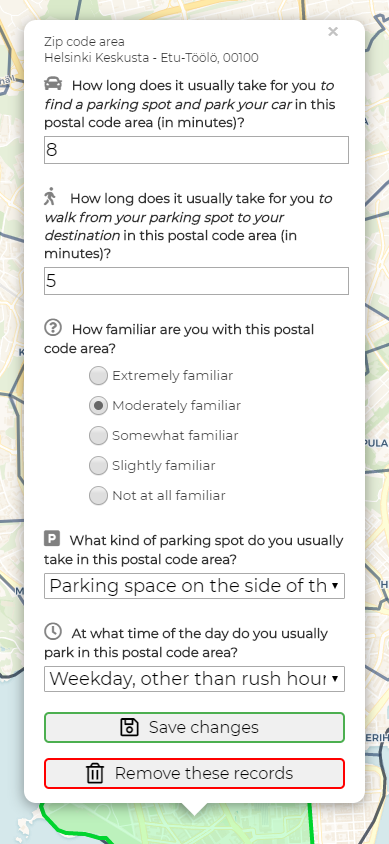
\includegraphics[width=6.25cm]{js_survey_en.png} }}%
    \qquad
    \subfloat[Survey questions in Finnish.]{{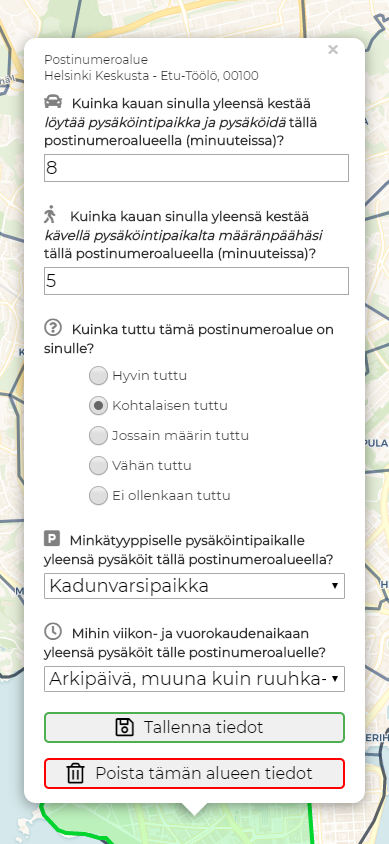
\includegraphics[width=6.25cm]{js_survey_fi.png} }}%
    \caption[Research survey questions in the web application]{For each postal code area of their choosing the respondent would answer to these five questions. The survey was made available in English and Finnish.}%
    \label{fig:js_survey_questions}%
\end{figure}

When data was received from the respondent, a script written in \gls{php} verified the data contents. This was an effort to prevent attacks on the web server running the study survey. Only specific variables of specific types were accepted from the front-end. Additionally, the \gls{php} verification made sure falsified or incomplete data would not be accepted into the database containing the verified results. If the server-side verification test failed in any way, the respondent was informed about it. 

In addition to the data verification, a PHP script tracked the IP addresses which accessed the survey web server. By using the survey, respondents agreed that their IP addresses were recorded for the use of this thesis solely to identify falsified or overlapping data and detect unique visits. All IP addresses were anonymised with a Python script and original sensitive data deleted. The anonymisation script is available for viewing at the thesis data analysis repository at GitHub (\textcolor{blue}{\url{https://github.com/sampoves/Msc-thesis-data-analysis}}).

As a final survey component, the server side contained two MySQL datatables, one for received data (table~\ref{tab:mysql_records}) and another for survey web page hits (table~\ref{tab:mysql_visitors}). In the table \textit{records}, the following data was recorded: time of sending (column name \code{timestamp}), IP address (\code{ip}), postal area code (\code{zipcode}), a value in the sequence 1--5 for the likert question (\code{likert}), a value in the sequence 1--5 for the question what type of parking spot was used (\code{parkspot}), an integer value for how long it usually took to park in this location (\code{parktime}), an integer value for how long it usually took to walk from parking place to one's destination (\code{walktime}), and a value in the sequence 1--4 for the question at what time of the day one usually parks in the location (\code{timeofday}) (table~\ref{tab:mysql_records_str}). In the table \textit{records}, it is notable that in the case an respondent sent the web server data for multiple postal code areas each of the postal code areas would take up their own row in the data table. Consequently, it was theoretically possible for one respondent to simultaneously submit 167 rows of data.

In the table \textit{visitors}, the following data was recorded: IP address (\code{ip}), the timestamp of the first visit of this IP address (\code{ts\_first}), the timestamp of latest visit of this IP address (\code{ts\_latest}), and the count of visits (\code{count}). In this table, an IP address is only stored once. On the first visit of an IP address, the row for that IP address is created in the data table with \code{ts\_first} and \code{ts\_latest} being identical. On further visits of that IP address the original row is appended with updated information in the columns \code{ts\_latest} and \code{count} (table~\ref{tab:mysql_visitors_str}).

\begin{hyphenrules}{nohyphenation}
    \begin{table}[H]
        \centering
        \setlength\tabcolsep{1.2ex}
        \caption[Structure of MySQL table records]{The structure of the survey MySQL table \textit{records} fetched with the statement \code{DESCRIBE records;}} 
        \label{tab:mysql_records_str}
        \begin{tabular}{ @{} >{\raggedright\arraybackslash}p{2cm} >{\raggedright\arraybackslash}p{2cm} >{\raggedright\arraybackslash}p{1cm} >{\raggedright\arraybackslash}p{1cm} >{\raggedright\arraybackslash}p{1.5cm} >{\raggedleft\arraybackslash}p{4cm} @{} }
            \toprule
            Field & Type & Null & Key & Default & Extra \\
            \midrule
            id & int(11) & No & PRI & NULL & AUTO\_INCREMENT \\
            timestamp & varchar(19) & Yes & & NULL & \\
            ip & TEXT & Yes & & NULL & \\
            zipcode & varchar(5) & Yes & & NULL & \\
            likert & int(1) & Yes & & NULL & \\
            parkspot & int(1) & Yes & & NULL & \\
            parktime & int(2) & Yes & & NULL & \\
            walktime & int(2) & Yes & & NULL & \\
            timeofday & int(1) & Yes & & NULL & \\
            \bottomrule
        \end{tabular}
    \end{table} 
\end{hyphenrules}

\begin{hyphenrules}{nohyphenation}
    \begin{table}[H]
        \centering
        \setlength\tabcolsep{1.2ex}
        \caption[Structure of MySQL table visitors]{The structure of the survey MySQL table \textit{visitors} fetched with the statement \code{DESCRIBE visitors;}} 
        \label{tab:mysql_visitors_str}
        \begin{tabular}{ @{} >{\raggedright\arraybackslash}p{2cm} >{\raggedright\arraybackslash}p{2cm} >{\raggedright\arraybackslash}p{1cm} >{\raggedright\arraybackslash}p{1cm} >{\raggedright\arraybackslash}p{1.5cm} >{\raggedleft\arraybackslash}p{4cm} @{} }
            \toprule
            Field & Type & Null & Key & Default & Extra \\
            \midrule
            id & int(11) & No & PRI & NULL & AUTO\_INCREMENT \\
            ip & TEXT & Yes & & NULL & \\
            ts\_first & DATETIME & Yes & & NULL & \\
            ts\_latest & DATETIME & Yes & & NULL & \\
            count & int(11) & Yes & & NULL & \\        
            \bottomrule
        \end{tabular}
    \end{table} 
\end{hyphenrules}

The parking survey was released to the public in May 2019 and the active phase of collecting data continued until 30th June 2019. However, the survey remained open after thiss active period, receiving the last row of data in October 2019. The majority of the respondents were found through Facebook. Invitations to participate in the survey were sent to 112 city district and neighborhood groups with a theoretical reach of tens of thousands of people. Of the 112 posts, 63 were Helsinki centric groups, while 22 were from Espoo, 15 from Vantaa, and 12 from municipalities bordering Helsinki Capital Region. In addition to these city district and municipal groups, invitation to participate was sent to two other Facebook groups, "Lisää kaupunkia Helsinkiin", a group for city planning ethusiasts in Helsinki, and the GIS profession group "GIS-velhot". It is not possible to conclusively differentiate from which group or city survey data originated from. A clue about the survey's popularity in each city, however, may be gained from the table \textit{visitors} due to the fact that invitation posts were sent over multiple days to the groups in the order: 

\begin{displayquote}
$\text{Espoo}\rightarrow\text{Helsinki}\rightarrow\text{Vantaa}\rightarrow\text{bordering municipalities}\rightarrow\text{reminders to the largest groups}$
\end{displayquote}

In addition to Facebook, an effort was also made to get faculty members of geosciences and geography and students of University of Helsinki to participate in the survey. A small amount of answers were collected with a tweet sent from the Twitter account of Digital Geography Lab. After the initial invitation to participate, reminders were sent to the largest Facebook groups one month after the original posts.

The source code for the survey described in this chapter and step-by-step information to set up an identical system is available at GitHub (\textcolor{blue}{\url{https://github.com/sampoves/parking-in-helsinki-region}}). As a side product, a variant of this survey was created where respondents pick precise points instead of areas. This point-based survey template is, too, available at GitHub (\textcolor{blue}{\url{https://github.com/sampoves/leaflet-map-survey-point}}). The parking survey web application as it was used in this thesis may be tested in the following web address: \textcolor{blue}{\url{https://parking-survey.socialsawblade.fi}}.

% \scalebox to prevent table going too wide
\begin{hyphenrules}{nohyphenation}
    \begin{table}[H]
        \centering
        \setlength\tabcolsep{2pt}
        \caption[MySQL table records]{An excerpt of the data content of the research survey MySQL table \textit{records}.} 
        \label{tab:mysql_records}
        \scalebox{0.9}
        {\begin{tabular}{ @{} >{\raggedright\arraybackslash}p{1.5cm} >{\raggedright\arraybackslash}p{4cm} >{\raggedright\arraybackslash}p{2.5cm} >{\raggedright\arraybackslash}p{2cm} >{\raggedright\arraybackslash}p{1.5cm} >{\raggedright\arraybackslash}p{1.5cm} >{\raggedright\arraybackslash}p{1.5cm} >{\raggedright\arraybackslash}p{1.5cm} >{\raggedright\arraybackslash}p{1.5cm} @{} }
            \toprule
            id & timestamp & ip & zipcode & likert & parkspot & parktime & walktime & timeofday \\
            \midrule
            3245 & 2019-06-06 21:41:21 & wro4qo8hv4 & 00510 & 1 & 4 & 0 & 3 & 1 \\
            3246 & 2019-06-06 21:41:54 & aonm72lyx3 & 00520 & 2 & 1 & 10 & 5 & 1 \\
            3247 & 2019-06-06 21:46:19 & n1982i4i2v & 00100 & 1 & 1 & 20 & 4 & 1 \\
            3248 & 2019-06-06 21:46:22 & sbhfz0uvsl & 00210 & 1 & 1 & 5 & 3 & 3 \\
            3249 & 2019-06-06 21:46:22 & sbhfz0uvsl & 00220 & 2 & 2 & 5 & 5 & 2 \\        
            \bottomrule
        \end{tabular}}
    \end{table} 
\end{hyphenrules}

\begin{hyphenrules}{nohyphenation}
    \begin{table}[H]
        \centering
        \setlength\tabcolsep{1pt}
        \caption[MySQL table visitors]{An excerpt of the data content of the research survey MySQL table \textit{visitors}.} 
        \label{tab:mysql_visitors}
        \begin{tabular}{ @{} >{\raggedright\arraybackslash}p{2cm} >{\raggedright\arraybackslash}p{3cm} >{\raggedright\arraybackslash}p{4cm} >{\raggedright\arraybackslash}p{4cm} >{\raggedleft\arraybackslash}p{1cm} @{} }
            \toprule
            id & ip & ts\_first & ts\_latest & count \\
            \midrule
            1780 & mvovd467a7 & 2019-05-26 15:25:23 & 2019-05-26 15:26:06 & 2 \\
            1781 & xgbgkkzxb3 & 2019-05-26 15:26:23 & 2019-05-26 15:26:23 & 1 \\
            1782 & c9qer4q99a & 2019-05-26 15:27:25 & 2019-05-26 15:27:25 & 1 \\
            1783 & cujhd0hng7 & 2019-05-26 15:27:29 & 2019-05-26 15:27:29 & 1 \\
            1784 & 3ja7gjtko6 & 2019-05-26 15:28:45 & 2019-05-26 15:29:20 & 2 \\        
            \bottomrule
        \end{tabular}
    \end{table} 
\end{hyphenrules}

\begin{figure}[H]%
    \centering
    \subfloat[Respondent arrives to the survey web application to see a map with the postal code areas of Helsinki Capital Region lined out.]{{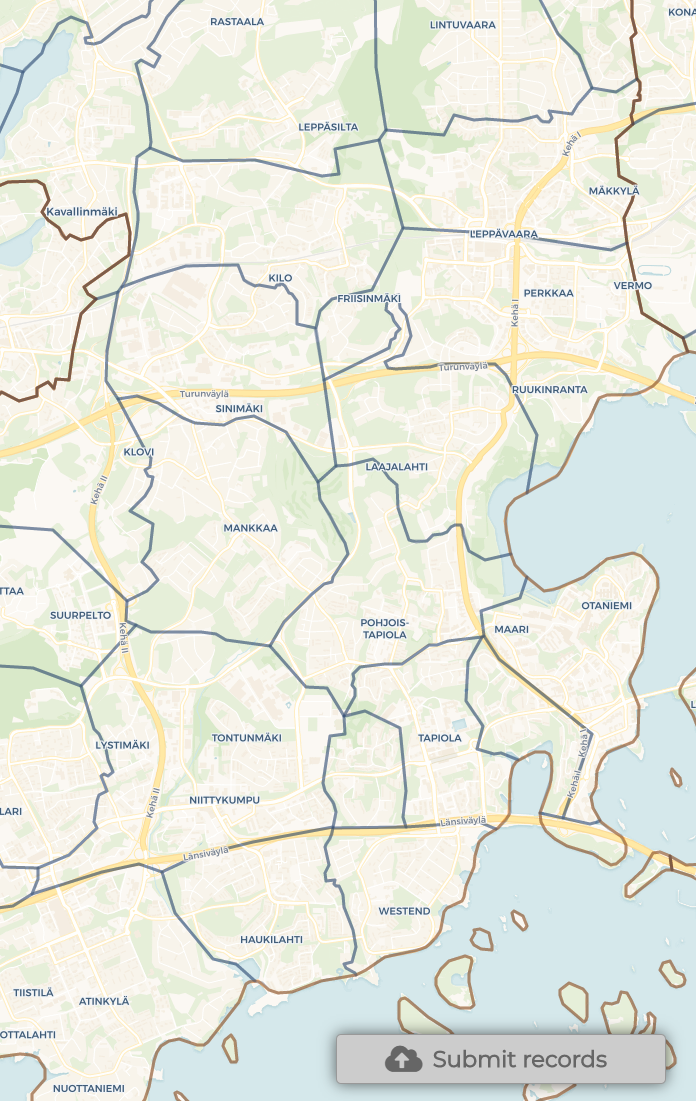
\includegraphics[width=7cm]{js_survey_process1.png} }}%
    \quad
    \subfloat[Respodent proceeds to fill out their parking experiences in freely chosen postal code areas.]{{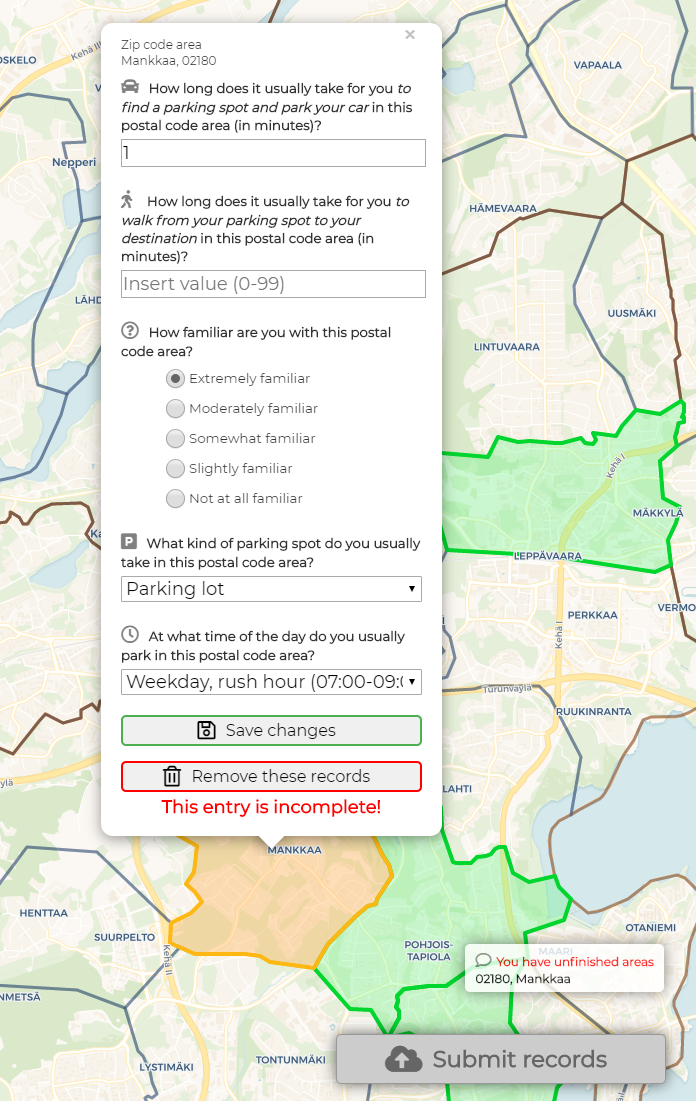
\includegraphics[width=7cm]{js_survey_process2.png} }}%
    \quad
    \subfloat[\textit{Submit records} button activates when all questions in all selected postal code areas are completed.]{{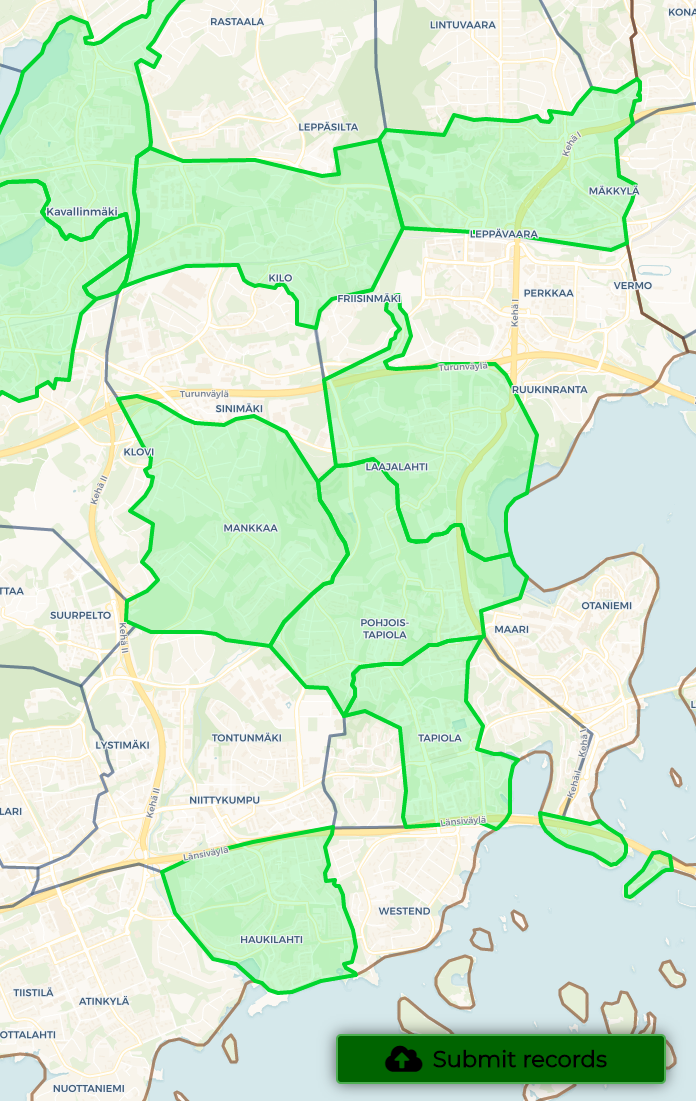
\includegraphics[width=7cm]{js_survey_process3.png} }}%
    \quad
    \subfloat[Respondent receives a prompt to confirm that their submission was successful.]{{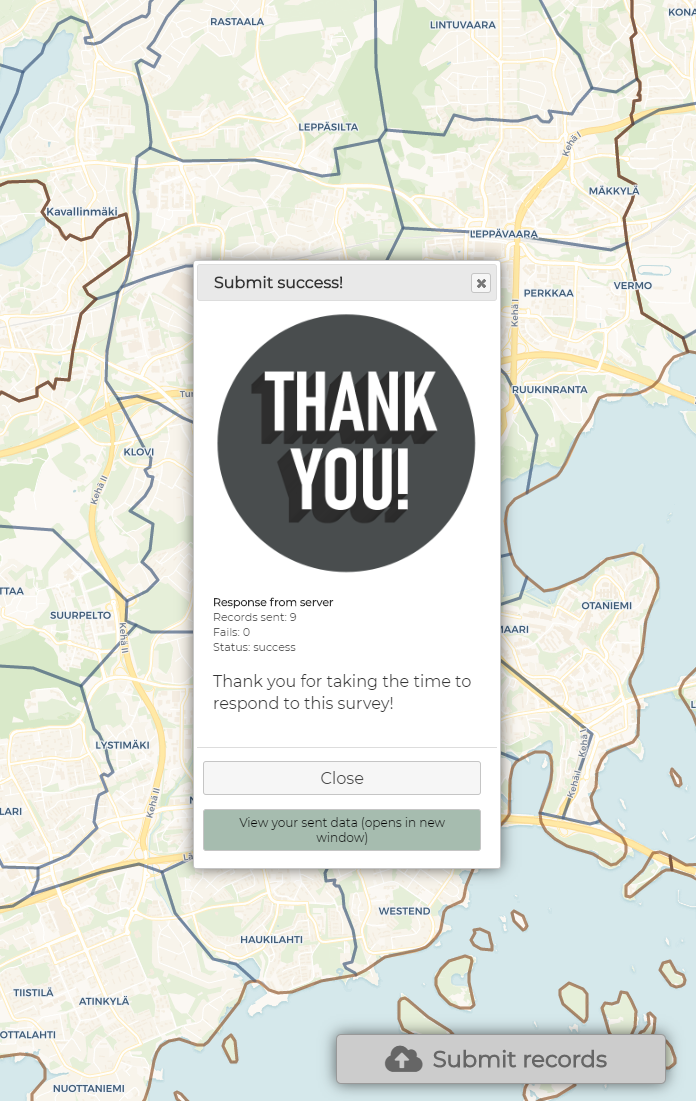
\includegraphics[width=7cm]{js_survey_process4.png} }}%
    \caption[Steps to fill out the survey]{A respondent would follow these steps to submit data through the survey web application.}%
    \label{fig:survey_process}%
\end{figure}

\newpage
\subsection{Processing survey data}
\label{sec:processdata} % labeling to enable hyperref to this chapter
\justify
%\begin{itemize} %processingin tärkeimmät kohdat
%    \item anonymisation of ip addresses
%    \item Read in spatial data sources
%    \item Read in survey data
%    \item Prepare source data (convert formats, remove some irregular erroneous answers from dataset)
%    \item Prepare shape files (remove islands not reachable by car)
%    \item give grid cells zipcodes (ykr grid does not have those of-the-shelf. Develop method to assign all cells zipcodes, take into account water and grid cells which are outside of research area)
%    \item respondent behaviour (see how each user has answered)
%    \item detect illegal data (first detect duplicate answers, produce report. Then remove data where parktime and/or walktime is 60 or over)
%    \item Add data to geodataframes (add columns for ykr\_vyoh, ua-forest, answer count, parktime and walktime mean
%    \item show statistics to user
%    \item Set percentage of urban zones and forest in each zipcode area (choose one urban zone and forest amount (jenks breaks) for every zipcode)
%    \item add subdivisions to data (all answer row gets corresponding subdivision value)
%    \item EXPERIMENTAL utilise travel-time matrix 2018, make comparisons
%    \item EXPERIMENTAL somehow create my own TTM18, with updated values
%    \item export results to R
%\end{itemize}

In this section, various data are refered to with abbreviated names as this makes it easier to follow the data processing workflow. Please see table~\ref{tab:used_data} for the key. \textcolor{red}{kaikki kohdat tässä kappaleessa ei käytä lyhenteitä (records, visitors, postal)}

The main objective of the thesis data processing was to merge survey responses (\textit{records}) with selected spatial data and prepare \textit{records}, survey visits (\textit{visitors}), \textit{postal}, and \textit{grid} for later analysis in R programming language environment. Using a selection of open spatial data (table~\ref{tab:used_data}), new explanatory variables would be available for use in the analysis. This opened opportunities to compare the newly gathered survey data against that in Helsinki Travel-time Matrix 2018. \textcolor{red}{toistoa} \textcolor{purple}{All data processing in this phase was carried out in Python programming language version 3.7.6, using Anaconda, a free and open-source Python distribution for scientific programming. Anaconda version 2020.02 included all essential packages for carrying out the script, with the exception of GeoPandas 0.5.0, the package for geospatial data manipulation in Python. GeoPandas and its dependencies -- GDAL 2.4.1, Fiona 1.8.6, pyproj 2.1.3, rtree 0.8.3, and Shapely 1.6.4.post1 -- were manually installed through Python package installer pip (table~\ref{tab:used_soft})}.

As the first step in the survey data processing, all IP addresses were anonymised and replaced with identifiers of ten characters consisting of numbers 0--9 and letters of English alphabet (figure~\ref{fig:gen_workflow}, section 1). The anonymisation was carried out in such a way that the random identifiers for respondents matched in both \textit{records} and \textit{visitors}, preserving the possibility to associate survey responses with survey visits. 

\begin{figure}[H]%
    \centering
    \subfloat[Unedited PAAVO postal code areas for Helsinki Capital Region.]{{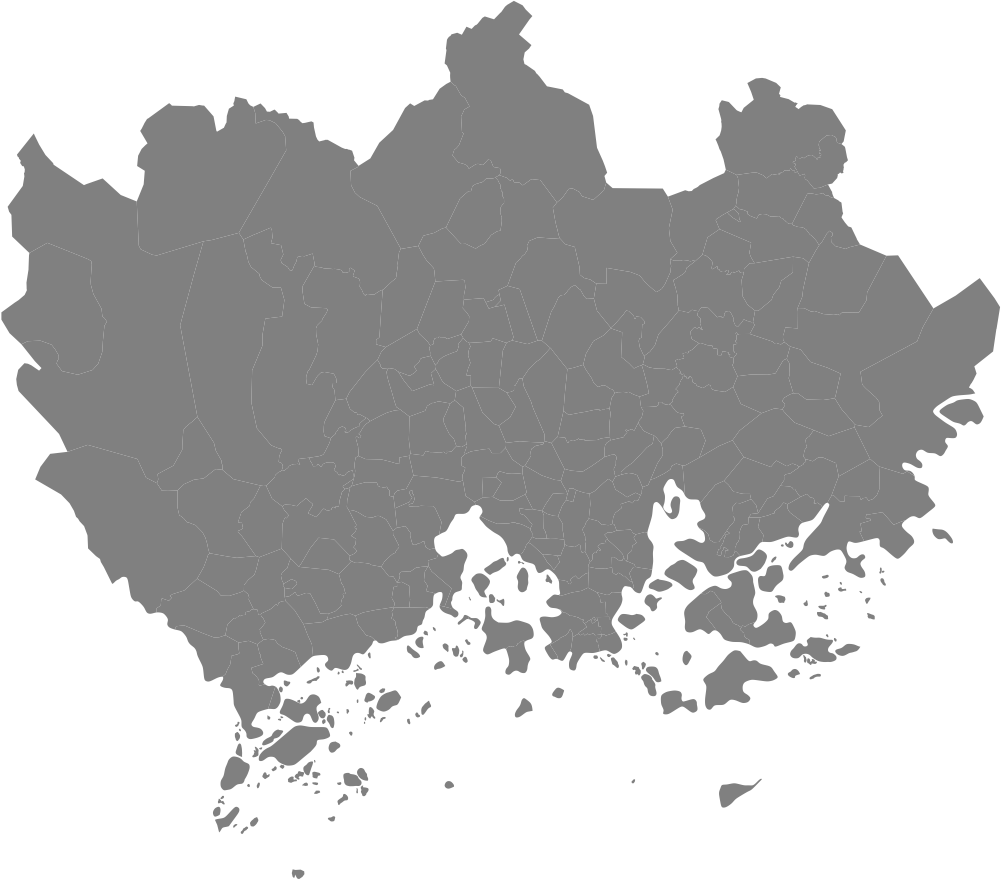
\includegraphics[width=8.1cm]{resarea_unedited.png} }}%
    \quad
    \subfloat[PAAVO postal code areas for Helsinki Capital Region, islands unreachable by car removed.]{{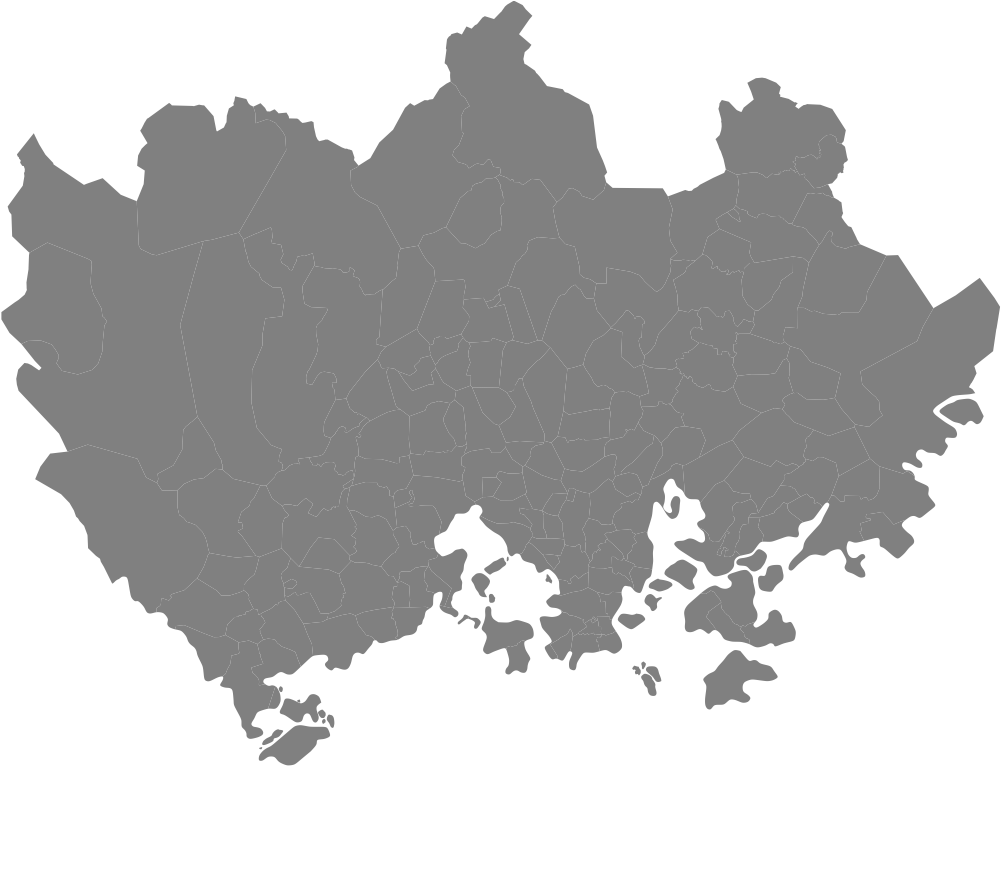
\includegraphics[width=8.1cm]{resarea_edited.png} }}%
    \caption[Process to remove islands not reachable by car]{Islands unreachable by car were removed from the postal code area data in the Python data processing.}%
    \label{fig:paavo_resarea}%
\end{figure}

The data processing proper started with loading the open spatial data presented in table~\ref{tab:used_data} and selecting only areas relevant to the research (figure~\ref{fig:gen_workflow}, section 2). For \textit{CORINE}, this meant selecting only areas marked Level1Eng, Artificial surfaces. \textit{YKR zones}, a dataset that covers the entirety of Finland, was clipped with spatial dimensions of PAAVO postal code areas data, \textit{postal}, that had been extended with a 500 meter buffer. \textit{postal} was processed to only include areas reachable by car from the mainland (figure~\ref{fig:paavo_resarea}). Islands not reachable by car were approximated visually using Google Maps and were removed from the data. However, some islands in Helsinki Capital Region are technically accessible with a car from the mainland, but in practice the access is limited. In these cases, deliberation was used. For example, Suomenlinna islands and Korkeasaari were kept in the data. Conversely, some technically car-accessible islands like Staffan in Espoo, and Mustasaari and Seurasaari in Helsinki were removed from the data with the grounds of them containing only private property, or no public parking spaces. \textcolor{red}{selitä laajemmin miksi näitä saaria poistellaan (analyysi ja visualisointi). lisäksi, mieti toi logiikka "yksityisalue tai ei yleisiä parkkiksia"}

\begin{figure}[H]%
    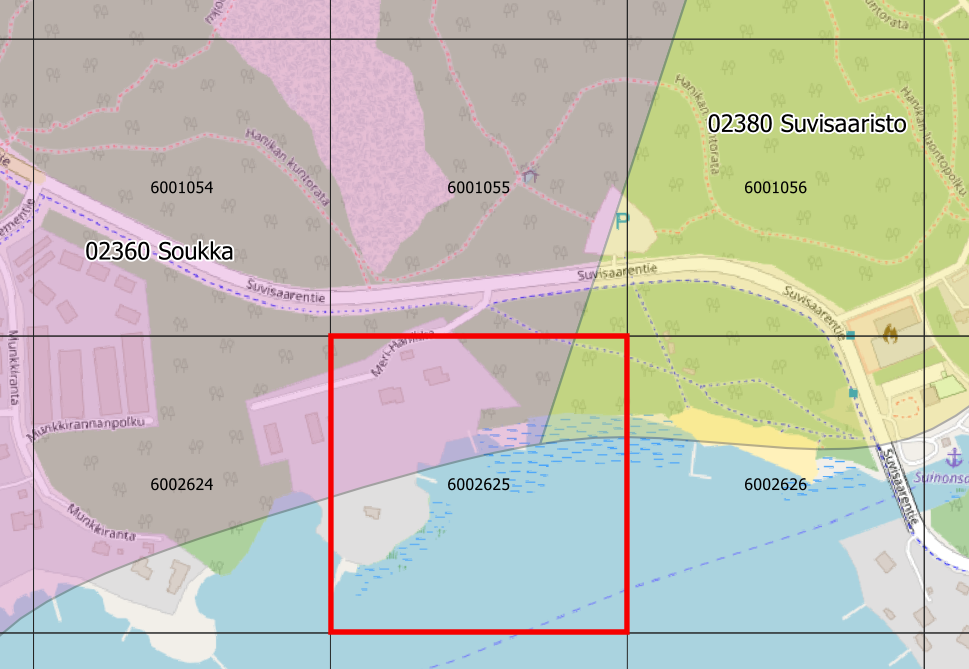
\includegraphics[width=\textwidth]{images/paavo-ykr.png}
    \caption[Assigning MetropAccess-YKR-grid postal codes]{The MetropAccess-YKR-grid cell 6002625 (marked with the red square) is assigned postal code 02360 because in that grid cell, the largest segment of PAAVO open data (coloured warm purple and yellow) belongs in the postal code 02360 Soukka. \textcolor{red}{osm cite}}%
    \label{fig:paavo_ykr}%
\end{figure}

Helsinki Region Travel Time Matrix 2018 and the survey data of this thesis operate in different spatial units. Travel time Matrix 2018 uses the MetropAccess-YKR-grid (\textit{grid}), a spatial dataset based on the Statistics Finland statistical grid with the cell size of 250 x 250 meters. The basic spatial unit of the survey data is the postal code area based on PAAVO open data (\textcolor{red}{lisää lähteet}). Using Python, postal codes were added to each \textit{grid} cell with the logic that the largest area in \textit{postal} (figure~\ref{fig:paavo_ykr}) assigns the postal code in each \textit{grid} cell. \textit{postal} polygons do not always intersect with the cells of \textit{grid} and because of this some cells were assigned a postal code of 99999 to denote missing data (\textcolor{red}{mieti vielä 99999:n käyttö}). As a side product of this postal code assignment, \textit{grid} was merged with data which tells how much of a cell was contained in the research area (\textit{postal}) and how large was the largest postal code area which dictated the postal code assignment of the current cell. \textcolor{red}{varmista että lukija ymmärtää PAAVO spatial datan ja tutkimusalueen yhteyden}

The data processing script created for this thesis contains detailed features to detect patterns in the survey data (figure~\ref{fig:gen_workflow}, section 3). To enhance pattern recognition, \textit{records} and \textit{visitors} were purged of known false data, which were namely responses and visits made by me.

The data processing script creates two distinct reports about \textit{records}. Firstly, the data processing script aggregates \textit{records} by IP address code, resulting in an Excel file where one row represents each respondent. It is then possible to review the behaviour of each respondent in detail. In addition to this report, the data processing script writes a text file report about IP address codes which submitted multiple responses from the same postal code area. The text file report also identifies whether the duplicate responses for each postal code area per each IP address code have identical values or if they have changed between responses. These two reports were used to determine what to do about the duplicates and values which appear anomalous.

It was decided that if the parking time or walking time value in a \textit{records} row was 60 minutes or greater, that data row would be deleted. This value is arbitrary. The research assumes that it is highly unlikely that anybody would generally park 60 minutes away from their final destination to which they would then proceed on foot. A hour of searching for parking is plausible in the center of Helsinki but because of its unlikeliness the same 60 minutes limit was utilised in searching for parking. It is not possible to determine why multiple survey responses contain the maximum value for parktime and walktime, 99, but it can not be ruled out that these data rows are protest votes meant to declare that reliable parking is hard to find in certain parts of Helsinki Capital Region. When advertising the thesis survey on Facebook, some people took the opportunity to voice their displeasure at the perceivedly difficult parking conditions in the Helsinki Capital Region. In conclusion, even though the Python script has the capability to delete data rows deemed illegal, all of the illegal data in \textit{records} was preserved a more versatile analysis in R.

Next in the survey data processing workflow the additional spatial data was added to \textit{postal}, the dataset with one row for each postal code area (figure~\ref{fig:gen_workflow}, section 4). Utilising \textit{records}, functions \code{sum}, \code{mean}, and \code{median} were used to produce answer count, and means and medians for parktime and walktime for all postal code areas. Each postal code area also received seven columns to depict the share of \textit{YKR zones} classes in percentage. It must be noted that before applying the \textit{YKR zones} data to the thesis data, classification in the source data was simplified with following the notation presented by the research group at the websites of the zones of urban structure (table~\ref{tab:ykr_zones_simplify}, \cite{FinnishEnvironmentInstitute2013}). Using \textit{CORINE} data, the percentage of artificial surface in each postal code area was calculated (table~\ref{tab:corine_artificial}).

\begin{hyphenrules}{nohyphenation}
    \begin{table}[H]
        \centering
        \def\arraystretch{1.2}
        \setlength\tabcolsep{1.2ex}
        \caption[YKR zones processing]{The logic by which the unedited source data for zones of urban structure was transformed for this thesis.}
        \label{tab:ykr_zones_simplify}
        \scalebox{0.9}
        {\begin{tabular}{ @{} >{\raggedright\arraybackslash}p{6cm} >{\raggedright\arraybackslash}p{6cm} @{} }
            \toprule
            Original definition & Definition for this thesis \\
            \midrule
            Keskustan jalankulkuvyöhyke & Keskustan jalankulkuvyöhyke \\
            \greyrule
            % Manually set the position of multirow label
            Keskustan reunavyöhyke & \multirow{3}{*}[-4.5ex]{Keskustan reunavyöhyke} \\
            Keskustan reunavyöhyke/intensiivinen joukkoliikenne & \\
            Keskustan reunavyöhyke/joukkoliikenne & \\
            \greyrule
            Alakeskuksen jalankulkuvyöhyke & \multirow{3}{*}[-4.5ex]{Alakeskuksen jalankulkuvyöhyke} \\
            Alakeskuksen jalankulkuvyöhyke/intensiivinen joukkoliikenne & \\
            Alakeskuksen jalankulkuvyöhyke/joukkoliikenne & \\
            \greyrule
            Intensiivinen joukkoliikennevyöhyke & Intensiivinen joukkoliikennevyöhyke \\ 
            \greyrule
            Joukkoliikennevyöhyke & Joukkoliikennevyöhyke \\
            \greyrule
            Autovyöhyke & Autovyöhyke \\
            \greyrule
            \textit{Areas not in the YKR zones data} & novalue \\
            \bottomrule
        \end{tabular}}
    \end{table} 
\end{hyphenrules}

\begin{hyphenrules}{nohyphenation}
    \begin{table}[H]
        \centering
        \def\arraystretch{1.2}
        \setlength\tabcolsep{1.2ex}
        \caption[CORINE data levels]{CORINE land cover 2018 data hierarchy under attribute data column Level1Eng, Artificial surfaces.}
        \label{tab:corine_artificial}
        \scalebox{0.85}
        {\begin{tabular}{ @{} >{\raggedright\arraybackslash}p{4cm} @{} >{\raggedright\arraybackslash}p{4cm} @{} >{\raggedright\arraybackslash}p{4.25cm} @{} >{\raggedright\arraybackslash}p{4cm} @{} }
            \toprule
            Level1, Level1Eng & Level2, Level2Eng & Level3, Level3Eng & Level4, Level4Eng \\
            \midrule
            \multirow{16}{4cm}[-15ex]{1 Artificial surfaces} & \multirow{2}{4cm}[-4ex]{11 Urban fabric} & 111 Continuous urban fabric 
 & 1111 Continuous urban fabric \\
            \arrayrulecolor{black!30}\cmidrule(lr){3-4}
            & & 112 Discontinuous urban fabric & 1121 Discontinuous urban fabric \\
            \arrayrulecolor{black!30}\cmidrule(lr){2-4}
            & \multirow{2}{4cm}[-0.5ex]{12 Urban fabric} & \multirow{2}{4cm}{121 Industrial or commercial units} & 1211 Commercial units \\
            \arrayrulecolor{black!30}\cmidrule(lr){4-4}
            & & & 1212 Industrial units \\
            \arrayrulecolor{black!30}\cmidrule(lr){2-4}
            & \multirow{3}{4cm}[-4ex]{12 Industrial, commercial and transport units} & 122 Road and rail networks and associated land & 1221 Road and rail networks and associated land \\
            \arrayrulecolor{black!30}\cmidrule(lr){3-4}
            & & 123 Port areas & 1231 Port areas \\
            \arrayrulecolor{black!30}\cmidrule(lr){3-4}
            & & 124 Airports & 1241 Airports \\
            \arrayrulecolor{black!30}\cmidrule(lr){2-4}
            & \multirow{4}{4cm}[-4ex]{13 Mine, dump and construction sites} & \multirow{2}{4cm}[-2.5ex]{131 Mineral extraction sites} & 1311 Mineral extraction sites \\
            \arrayrulecolor{black!30}\cmidrule(lr){4-4}
            & & & 1312 Open cast mines \\
            \arrayrulecolor{black!30}\cmidrule(lr){3-4}
            & & 132 Dump sites & 1321 Dump sites \\
            \arrayrulecolor{black!30}\cmidrule(lr){3-4}
            & & 133 Construction sites & 1331 Construction sites \\
            \arrayrulecolor{black!30}\cmidrule(lr){2-4}
            & \multirow{5}{4cm}[-2ex]{14 Artificial, non-agricultural vegetated areas} & 141 Green urban areas & 1411 Green urban areas \\
            \arrayrulecolor{black!30}\cmidrule(lr){3-4}
            & & \multirow{4}{4cm}[-3ex]{142 Sport and leisure facilities} & 1421 Summer cottages \\
            \arrayrulecolor{black!30}\cmidrule(lr){4-4}
            & & & 1422 Sport and leisure areas \\
            \arrayrulecolor{black!30}\cmidrule(lr){4-4}
            & & & 1423 Golf courses \\
            \arrayrulecolor{black!30}\cmidrule(lr){4-4}
            & & & 1424 Race courses \\
            \bottomrule
        \end{tabular}}
    \end{table} 
\end{hyphenrules}

% https://www.spatialanalysisonline.com/HTML/index.html?classification_and_clustering.htm
In the finalising section, \textit{records} was prepared for analysis and visualisation in R (figure~\ref{fig:gen_workflow}, section 5). The software library for plotting in R, \textit{ggplot2}, prefers data inputted in long format. To study charasteristics of postal code areas in this research, it meant adding repetitive data columns in \textit{records}, where values for CORINE land cover 2018 artificial surfaces, YKR zone and subdivision remained unchanged for all rows in the same postal code area. For artificial surfaces, a custom Jenks natural breaks function (GitHub user Drewda, \textcolor{red}{add cite, add jenks cite, kato kommenttilinkki}) with five classes were utilised to find the applicable Jenks breaks class for each postal code area. For YKR zones, the most common urban structure type in percentage was selected for each postal code area. In addition, \textit{records} was inserted with municipality subdivision information (figure~\ref{fig:subdiv_placement}). This was achieved by collecting data from the web sites of the municipalities of Helsinki Capital Region (\cite{Espoonkaupunki2020}, \cite{Helsinginkaupunkiymparistontoimiala2019}, \cite{Vantaankaupunki2019}). In these sources, each municipality broke the subdivisions down to city district level, from where it was possible to allot each postal code area with a subdivision. This was for the most part simplistic work, but in some cases the postal code areas and city districts did not align and author's own deliberation was used to help the placement. Some of the most glaring discrepancies between PAAVO postal code areas and subdivision boundaries occur in Espoo. In the case of Lippajärvi-Järvenperä, a postal code area north of Kauniainen, the subdivision Vanha-Espoo was chosen because Lippajärvi-Järvenperä as a whole does not fit into the charasteristics of Suur-Leppävaara, and at the same time the city districts Lippajärvi and Järvenperä do not fit into the distinctive features of the subdivision Pohjois-Espoo. In the same spirit the postal code area Sepänkylä-Kuurinniitty south of Kauniainen lies troublingly in the area of four subdivisions of Espoo. In the end Vanha-Espoo was chosen as Sepänkylä-Kuurinniitty lies for the most part in its area. Similar complications occurred in Helsinki and Vantaa (the partial placement of Kirkonkylä-Veromäki and Ruskeasanta-Ilola in subdivision of Tikkurila) and using my best judgement, the classification shown in figure~\ref{fig:subdiv_placement} was used in the survey results analysis of this thesis.

The source code for the data processing described in this chapter is available at GitHub (\textcolor{blue}{\url{https://github.com/sampoves/Msc-thesis-data-analysis}}).

\begin{figure}[H]%
    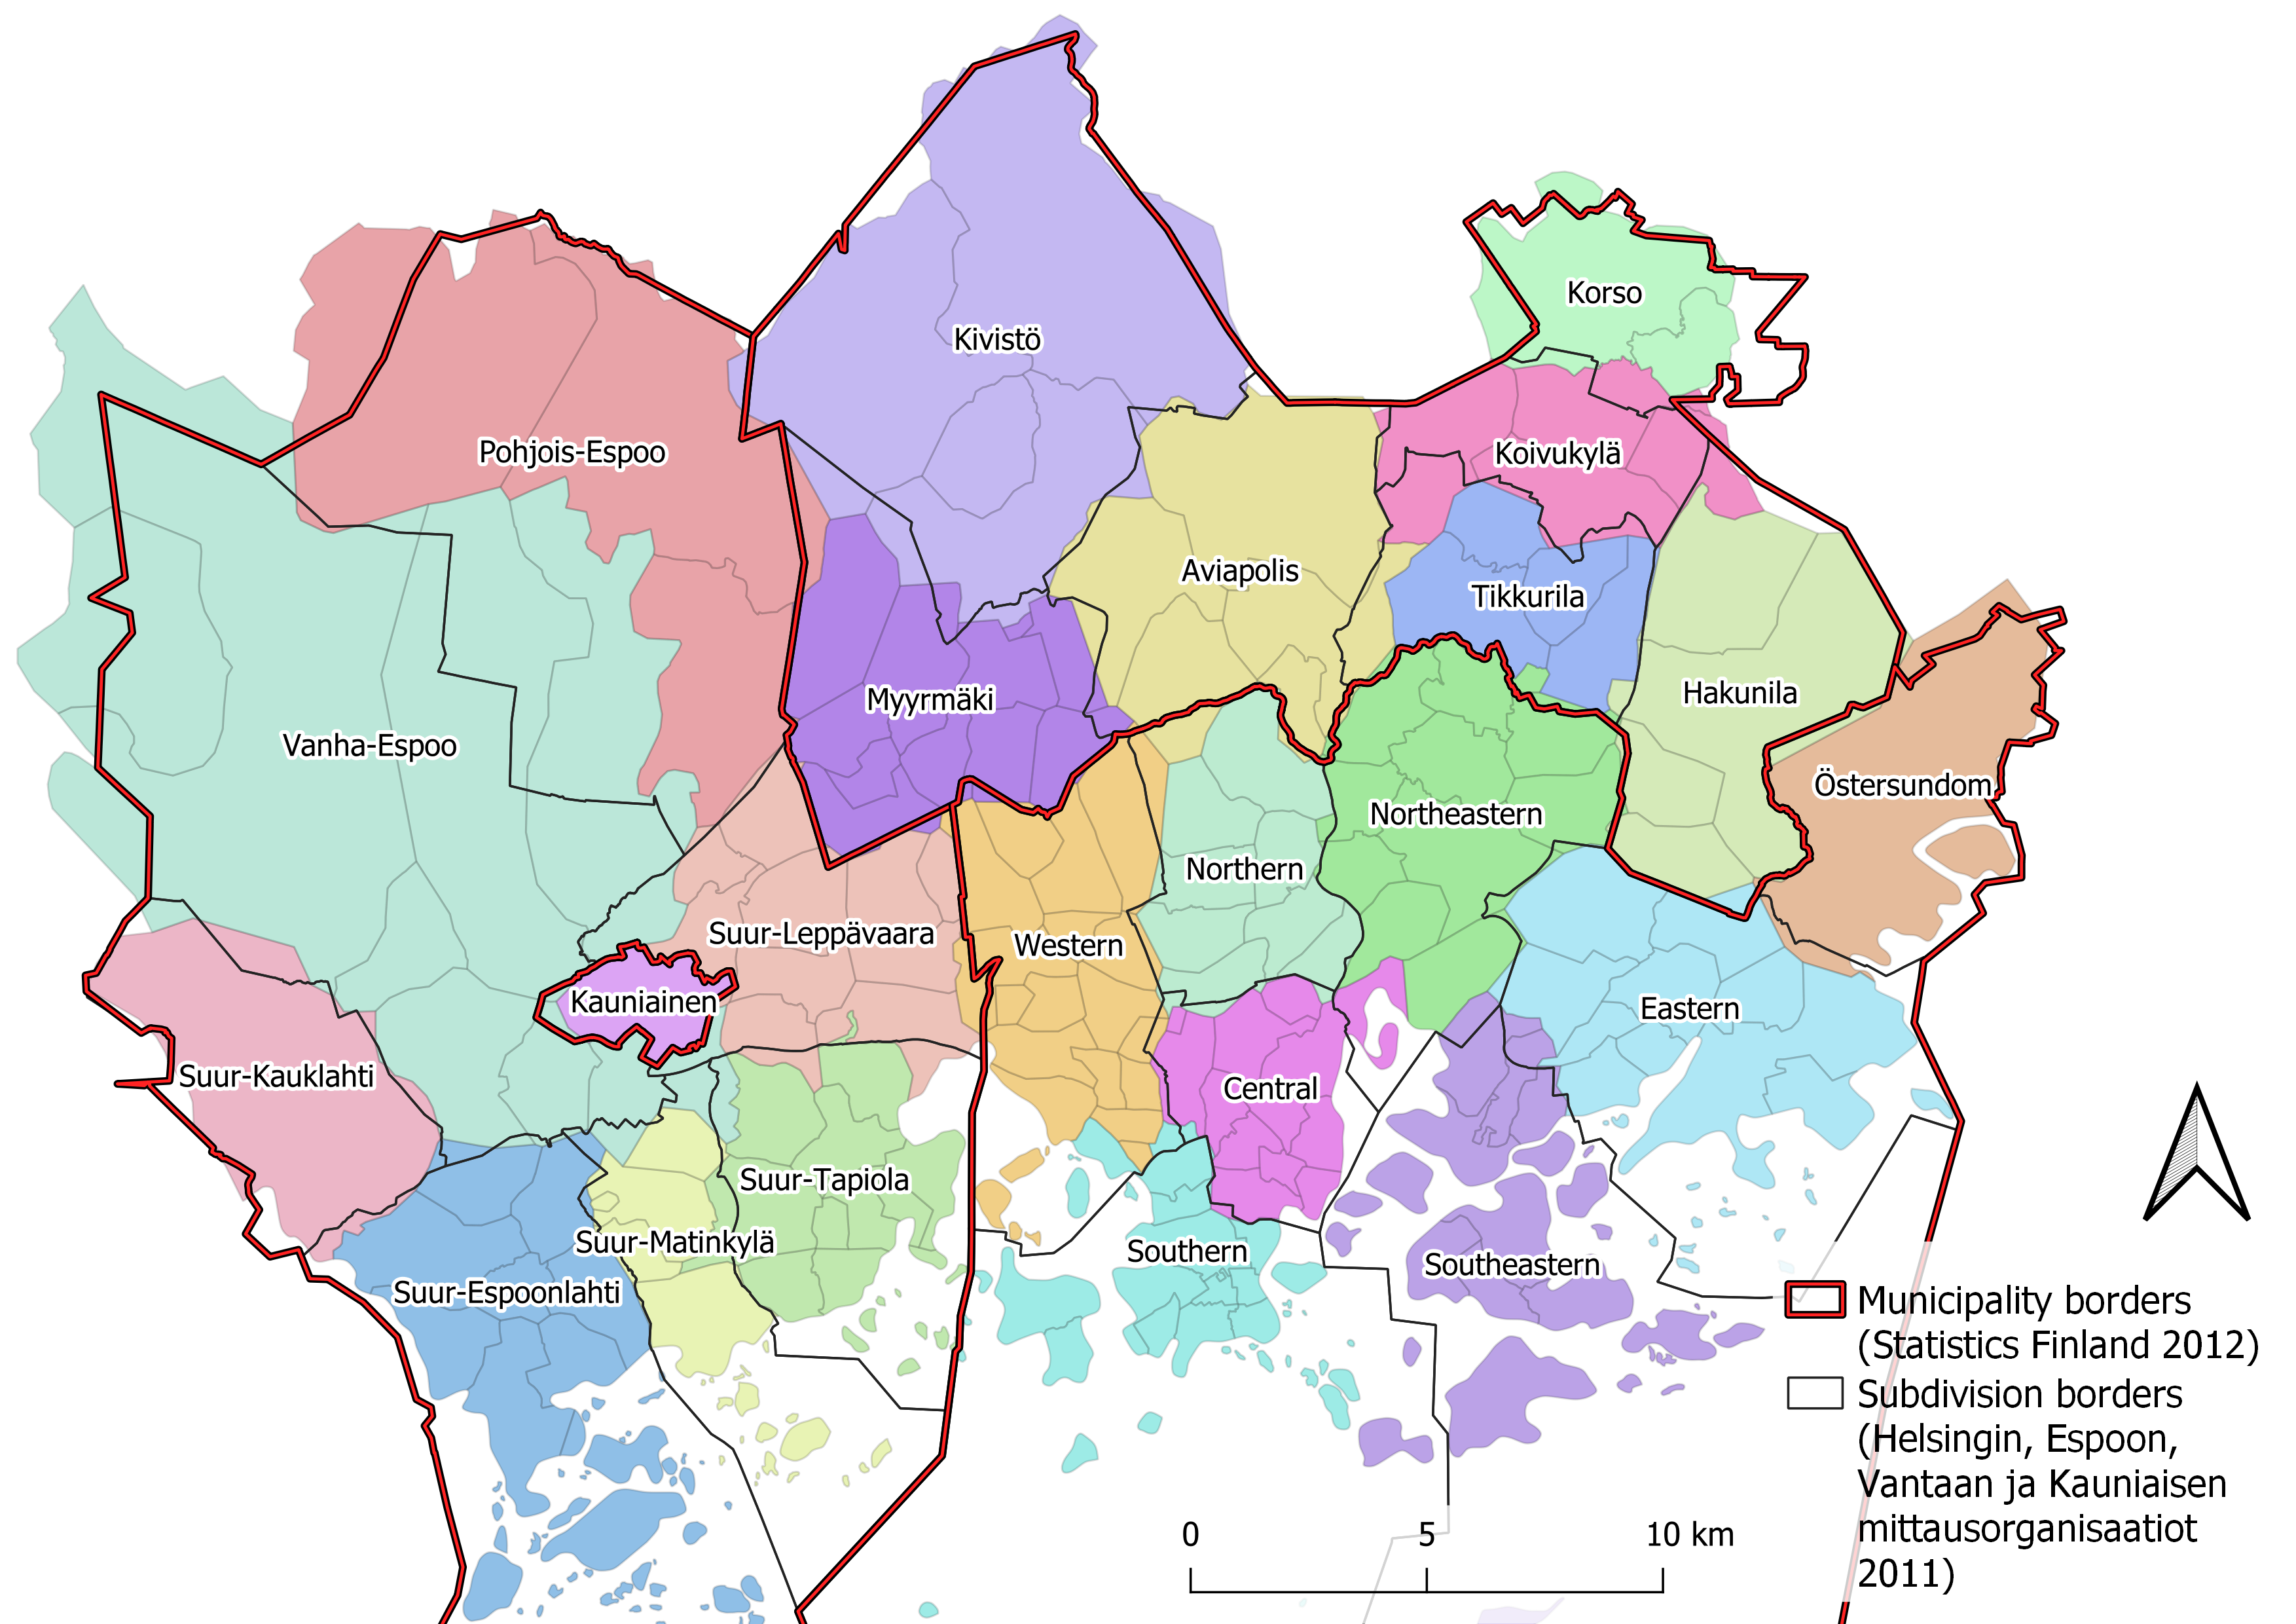
\includegraphics[width=\textwidth]{images/thesis_subdiv_place.png}
    \caption[Placing postal code areas in subdivisions]{For the purposes of analysis in R, all postal code areas in \textit{postal} were assigned with subdivision information. In this figure, distinct colors depict the postal code areas with the subdivision classification chosen for this thesis.}%
    \label{fig:subdiv_placement}%
\end{figure}

\newpage
\subsection{Creating applications and conducting analyses}
\subsubsection{Analysis application}
\justify
%\begin{itemize}
%    \item Prepare data to R compliant format
%    \item ShinyApp descriptive statistics
%    \item shinyapp histogram for parktime and walktime
%    \item shinyapp boxplot, show outliers
%    \item shinyapp barplot, show amounts
%    \item shinyapp levene test
%    \item shinyapp one-way anova
%    \item shinyapp map, nice to have, not at all important
%    \item visitor shinyapp, see the accumulation of visits and received records
%\end{itemize}

Once the data processing in Python was completed, \textit{records} and \textit{visitors} were carried over to R to utilise its easy to access statistical analysis functionality. For this thesis, this meant namely packages \textit{onewaytests} for ANOVA and Brown-Forsythe test, \textit{plotrix} for standard error, and \textit{moments} for quantiles (table~\ref{tab:used_soft}). To help study the large datasets, three Shiny applications were written, one for \textit{records} and a second for \textit{visitors}, and a third one to study differences between the thesis survey results and Helsinki Region Travel Time Matrix 2018. Benefits in creating these applications were twofold. Firstly, approaching the survey results from an interactive perspective allowed countless combinations of active and inactive variables -- without constant tweaking of code -- which would be beneficial for the analysis of \textit{records}. Secondly, programming the applications using Shiny enabled the use of shinyapps.io, a service where one can host Shiny applications on the internet without charge. Combination of these two factors made it effortless to analyse results of the survey in a visual way and at the same time, publish the tools and results to the public, upholding the thesis' mission of openness and transparency.

\begin{figure}[H]%
    \centering
    \subfloat[A segment of the shinyapps.io deployment of \textit{records} application. The web application provides a wide array of analysis and visualisation tools for the results of the thesis survey research.]{{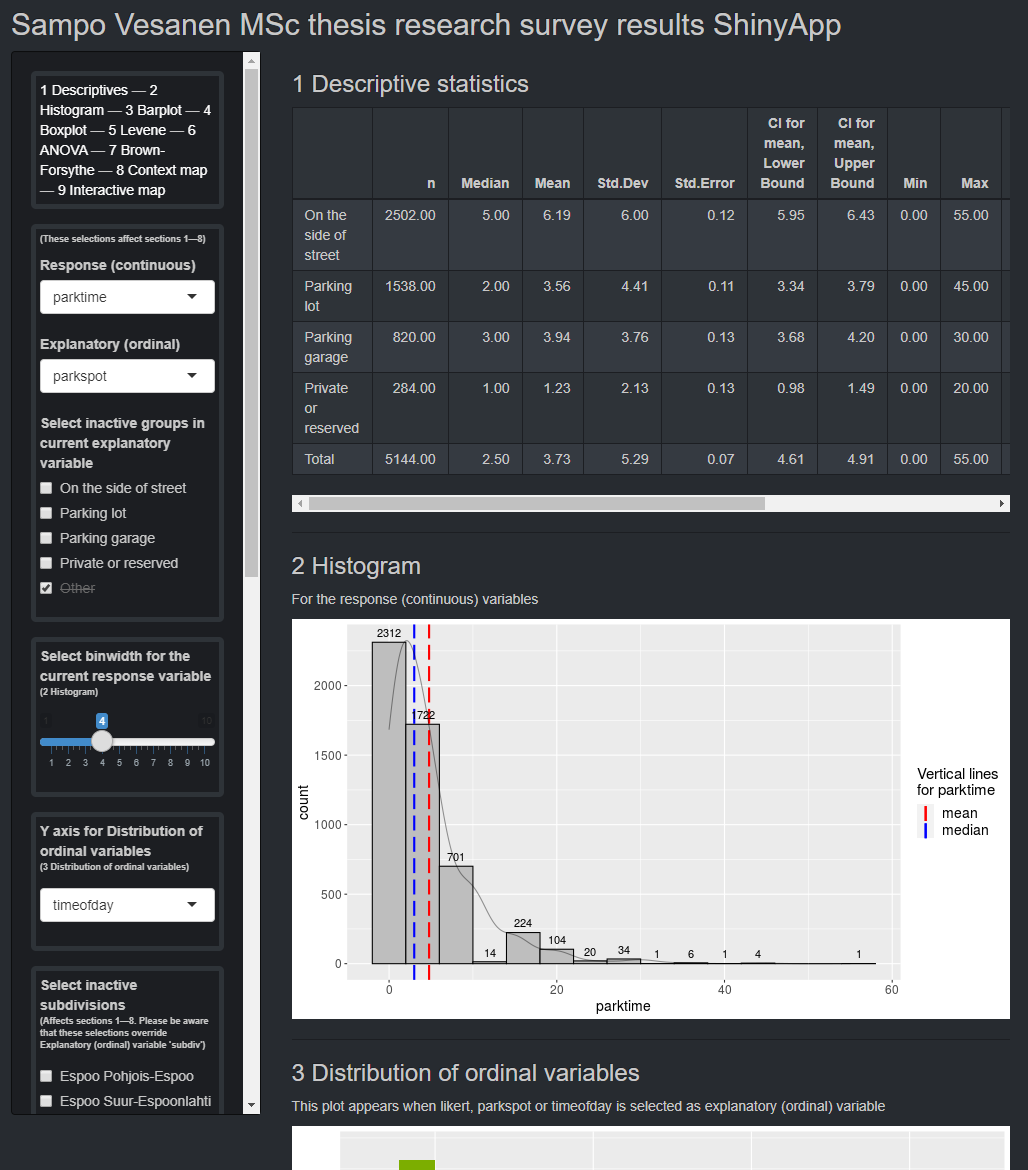
\includegraphics[width=8.1cm]{images/shinyapps_analysis.png} }}%
    \quad
    \subfloat[The shinyapps.io deployment of \textit{visitors} application. In this web application users may examine how the amounts of submitted responses and unique first visits to the thesis web survey developed over time.]{{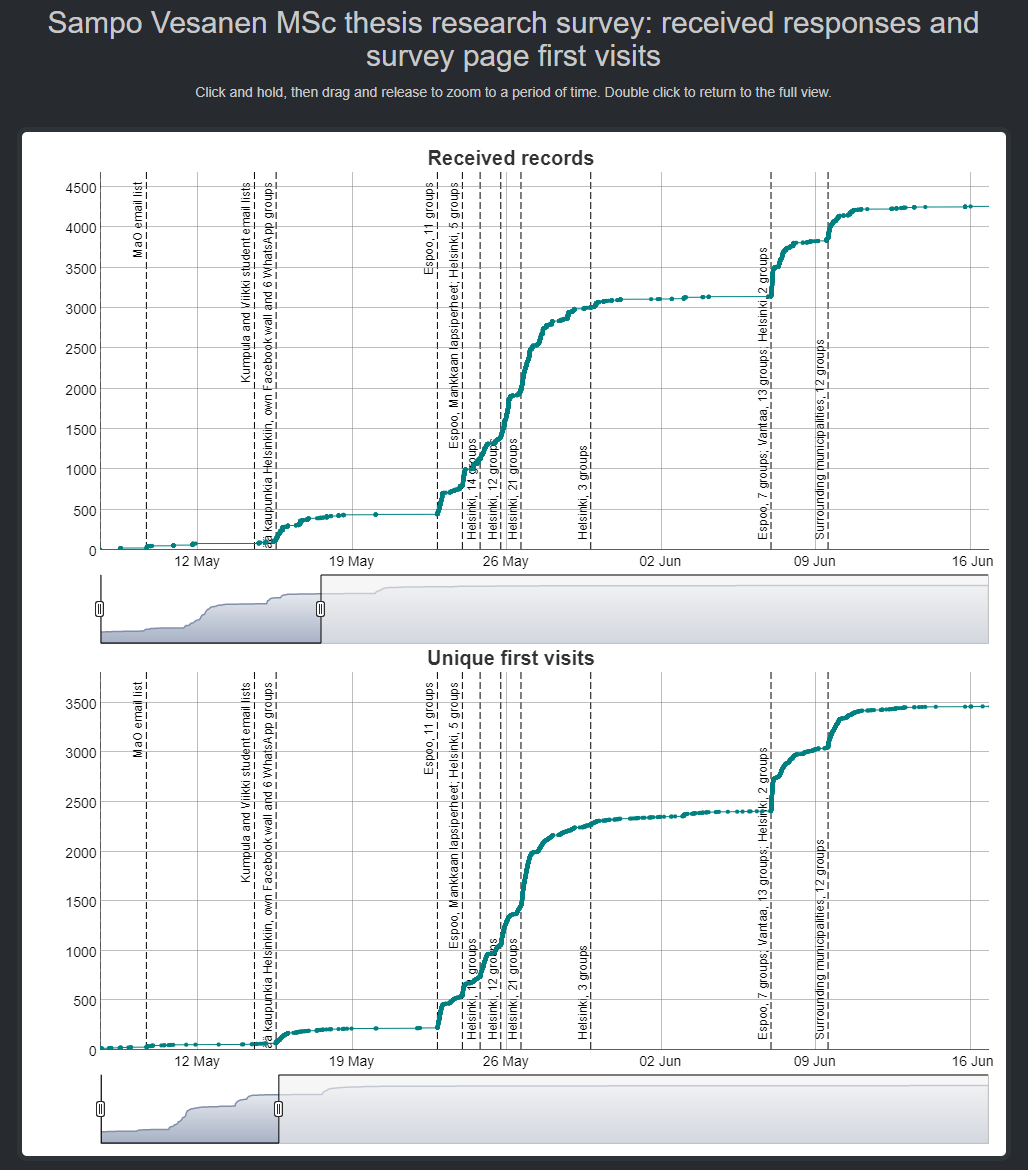
\includegraphics[width=8.1cm]{images/shinyapps_visitors.png} }}%
    \caption[Survey results as shinyapps.io web applications]{shinyapps.io deployments of the two survey dataset analysis applications.}%
    \label{fig:shinyapps}%
\end{figure}

In the Shiny application for \textit{records}, users can view the survey responses from many different angles. Users are given control which variables are active at any moment (\hyperref[fig:shinyapps]{figure~\ref{fig:shinyapps}a}). Users control the variables through the side panel, with settings taking effect in the main panel. The variables currently viewed are selected through two dropdown menus, Response (continuous) and Explanatory (ordinal). Continuous variables are \code{parktime} and \code{walktime} with an integer range 0--99. Available ordinal variables are \code{likert}, \code{parkspot}, \code{timeofday}, \code{artificial}, \code{ykr\_zone}, and \code{subdiv} with the values that can not be unequivocally ordered in a sequence in the same way as continuous variables. One variable from each variable group can be selected at the same time. Any and all groups of values in the ordinal variables can be deactivated to better understand the significance of each value group. In addition to the selection of the continuous and ordinal variable, users can deactivate \textit{records} data rows based on their spatial location in municipality subdivisions assigned in \hyperref[sec:processdata]{\fullref{sec:processdata}}. Most importantly, the analysis application allows selection of maximum allowed value for \code{parktime} and \code{walktime}. The default value for both is set at 59 minutes, as discussed in the \fullref{sec:processdata}, but the user is free to choose any value between zero and 99.

% levene, anova, boxplot, lue: https://www.itl.nist.gov/div898/handbook/eda/section3/eda35a.htm. On legit lähde
\begin{table}[H]
    \centering
    \caption[Records Shiny application features]{\textit{Records} Shiny application features. All features are affected by the maximum permitted \code{parktime} and \code{walktime} values, currently active response and explanatory variables and inactive subdivisions. In addition, certain exclusive settings are found in some of the features.}
    \label{tab:records_shiny_features}
    \scalebox{0.8}
    {\def\arraystretch{1.3}
    \setlength\tabcolsep{1.2ex}
    \begin{tabular}{ @{} >{\raggedright\arraybackslash}p{3cm} >{\raggedright\arraybackslash}p{2cm} >{\raggedright\arraybackslash}p{6cm} >{\raggedright\arraybackslash}p{6cm} @{} }
        \toprule
        Feature & Type & Outputs & Feature exclusive settings \\
        \midrule
        1 Descriptive statistics & Analysis, table & n, median, mean, standard deviation, standard error, confidence interval for mean, lower bound, confidence interval for mean, min, max, 25th quartile, 75th quartile, skewness, kurtosis & None \\
        2 Histogram & Analysis, chart & Histogram, kernel density estimate, mean, median & Histogram binwidth \\
        3 Distribution of ordinal variables & Analysis, chart & Distribution plot by explanatory variable value group & Explanatory variable for the distribution plot Y axis \\
        4 Boxplot & Analysis, chart & Quartile data & None \\
        5 Test of homogeneity of variances (Levene's test) & Analysis, table & Equality of variances for a variable calculated for the currently active response and explanatory variable & None \\
        6 Analysis of variance (ANOVA) & Analysis, table & Analysis of differences among group means in a sample & None \\
        7 Brown-Forsythe test & Analysis, table & Analysis of equality of group variances & None \\
        8 Interactive map & Visualisation, map & Choropleth map with Jenks breaks classifiction, descriptive data per postal code area (answer count, mean and median for parktime and walktime, forest amount percentage, largest YKR zone percentage) & - Selection of active municipalities \linebreak - Jenks breaks parameter column \linebreak - Amount of Jenks breaks classes \linebreak - Possibility to visualise the map with boundaries and labels \\
        \bottomrule
    \end{tabular}}
\end{table} 

When the user has selected a continuous and an ordinal variable to compare, they are presented a thorough set of descriptive statistics for the currently active data rows with n, median, mean, standard deviation, standard error, confidence interval for lower and upper bound, minimum and maximum, 25 \% and 75 \% quantiles, skewness, and kurtosis (table~\ref{tab:records_shiny_features}). For the continuous variables, a histogram is available to visualise the distribution of \code{walktime} and \code{parktime}. Distribution of ordinal variables \code{likert}, \code{parkspot}, and \code{timeofday} can be compared against other ordinal variables in a barplot. To study quartiles, a boxplot is available. Importantly, users can test their selection of variables with the test of homogeneity of variables (Levene's test), analysis of variance (ANOVA), and the Brown-Forsythe test \textcolor{red}{laajenna selityksiä}. Lastly, a versatile interactive map of the research area is provided. This map, divided in postal code areas, reveals the survey results in a spatial fashion. The interactive map is affected by the maximum parking time and walking time, selection of an ordinal variable and any inactive subdivisions to provide a flexible view into the details of the data. In addition, this interactive map is controlled by some exclusive settings of its own. The interactive map settings offers six distinct parameters for viewing the research area through Jenks natural breaks classification, alongside with the possibility to select the amount of classes in the map view. Hovering the cursor over the map reveals a tooltip which the application users can use to view mean, median, and percentage data about each postal code area in Helsinki Capital Region. Tooltips are also available for the barplot of distribution of ordinal variables and the boxplot.

Much additional work was put into the analysis application to make it as clear and easy to use as possible. The application features a number of links to move between the features and the settings, while smooth scrolling and animations help in directing the attention of the user. Each application feature can be switched on and off to make space for exactly the topic the user wants to examine. The analysis application allows downloading all the results, outputting tables into comma separated value files (CSV). Charts and the map are outputted into high resolution images (PNG). \textcolor{red}{too much detail?} \textcolor{purple}{The files are intuitively named informing of the used application settings and the date of file download. In case ordinal variable value groups or subdivisions are turned off, the output images are appended with an appropriate notification.} Attention was given to ensure the usage of the analysis application on mobile phones. To this end, the CSS style sheet of the application detects mobile phone screen sizes and adjusts the application content accordingly. The sidebar tends to block the view of the main panel on mobile screens and for this situation a switch is provided to hide the sidebar at any given time. All graphical elements of the application are in SVG (Scalable Vector Graphics) format which supports effortless zooming without loss of detail.

The source code for the \textit{records} analysis application is available at GitHub (\textcolor{blue}{\url{https://github.com/sampoves/thesis-records-shinyapps}}). The application may be viewed on shinyapps.io (\textcolor{blue}{\url{https://sampoves.shinyapps.io/records}}).

\subsubsection{Visitors application}

In the Shiny application for \textit{visitors}, users can examine events in the timeline of the survey research (figure~\ref{fig:shinyapps}). In this interactive view, cumulative charts are presented for received survey responses and survey page first visits. The charts reveal the effect and importance of advertisement on actual received responses and survey traffic. While not completely verifiable, the significance of different sources of responses can be viewed in the application.

Compared to the other two analysis applications programmed for this thesis, the \textit{visitors} application is relatively simple in its function and features. The user controls the chart view with mouse clicks or dragging the cursor and no additional settings are provided.

The source code for the \textit{visitors} analysis application is available at GitHub (\textcolor{blue}{\url{https://github.com/sampoves/thesis-visitors-shinyapps}}). The application may be viewed on shinyapps.io (\textcolor{blue}{\url{https://sampoves.shinyapps.io/visitors}}).

\subsubsection{Travel time comparison application}

Despite potential for extensive analysis, the applications described in previous chapters do not provide means to study the third research question of this thesis:

\begin{displayquote}
III What is the significance of the parking process to the overall travel time?
\end{displayquote}

To answer this research question, an application to compare travel time datasets was programmed (figure~\ref{fig:shinyapps_comparison}). In this application, the user can view a variety of descriptive values calculated from Helsinki Region Travel Time Matrix 2018, the thesis survey data, and a dataset created by comparing the two other datasets. The user is given control a set of features, such as the travel times origin postal area code, a parameter to visualise on the map, and the amount of symbology classes. The map view can be customised with a number of visualisation options, such as visible regional boundaries and physical features (inland water, main roads), and options for the labelling of postal code areas.

It was decided that the basic spatial unit for the comparison application would be the PAAVO postal code area as the thesis survey results exist in that resolution. This decision necessitated extensive processing of \textit{TTM} data. Firstly, the application needed to be able to recalculate the map view as quickly as possible. Secondly, the original \textit{TTM} dataset is unwieldy to be used in its original format in a web application (data stored in uncompressed txt files, data scope much too detailed for the application). Thirdly, the hosting service shinyapps.io places technical limitations on the resource intensity of the application. For these three main reasons, the library fst (table~\ref{tab:used_soft}) was first used to convert the \textit{TTM} private car columns into the data format used by the library (table~\ref{tab:comparison_fst1}), and then using the dataset \textit{grid} preprocessed in Python to aggregate all \textit{TTM} grid cell values to the PAAVO postal code area level and writing the results using the optimised fst format (table~\ref{tab:comparison_fst2}). For data completeness, \textit{TTM} searching for parking (0.42 minutes) and walking to destination (2.0--2.5 minutes) data was added to these aggregated \textit{TTM} files. This aggregation method drastically reduced unnecessary processing, minimised disk space needed, and kept application memory footprint in manageable figures for the deployment to the internet. The other main dataset used in the comparison application, the thesis survey data, is aggregated to postal code area level each time the application initialises, as the complete survey results dataset is miniscule in size compared to \textit{TTM}.

\begin{hyphenrules}{nohyphenation}
    \begin{table}[H]
        \centering
        \setlength\tabcolsep{1pt}
        \caption[Comparison application fst structure I]{An excerpt of the data content of \textit{TTM} converted to fst format for further processing (table~\ref{tab:comparison_fst2}). Original file 5785xxx/travel\_times\_to\_ 5785640.txt.} 
        \label{tab:comparison_fst1}
        \begin{tabular}{ @{} >{\raggedright\arraybackslash}p{1cm} >{\raggedright\arraybackslash}p{2cm} >{\raggedright\arraybackslash}p{2cm} >{\raggedright\arraybackslash}p{2cm} >{\raggedright\arraybackslash}p{2cm} >{\raggedright\arraybackslash}p{2cm} @{} }
            \toprule
            & from\_id & to\_id & car\_r\_t & car\_m\_t & car\_sl\_t \\
            \midrule
            10 & 5787549 & 5785640 & 22 & 21 & 16 \\
            11 & 5787550 & 5785640 & 22 & 21 & 16 \\
            12 & 5789447 & 5785640 & 10 & 9 & 8 \\
            13 & 5789448 & 5785640 & 10 & 9 & 8 \\
            14 & 5789449 & 5785640 & 11 & 10 & 9 \\
            \bottomrule
        \end{tabular}
    \end{table} 
\end{hyphenrules}

\begin{hyphenrules}{nohyphenation}
    \begin{table}[H]
        \centering
        \setlength\tabcolsep{5pt}
        \caption[Comparison application fst structure II]{An excerpt of the data content of \textit{TTM} aggregated to postal code area level for the use of the comparison application. The origin postal code area of the shown data table is 00100 Helsinki Keskusta -- Etu-Töölö.} 
        \label{tab:comparison_fst2}
        \begin{tabular}{ @{} >{\raggedright\arraybackslash}p{1cm} >{\raggedright\arraybackslash}p{1.5cm} >{\raggedright\arraybackslash}p{1.5cm} >{\raggedright\arraybackslash}p{2cm} >{\raggedright\arraybackslash}p{2cm} >{\raggedright\arraybackslash}p{2cm} >{\raggedright\arraybackslash}p{2cm} >{\raggedright\arraybackslash}p{2cm} @{} }
            \toprule
            & zipcode & from\_zip & ttm\_r\_avg & ttm\_m\_avg & ttm\_sl\_avg & ttm\_wtd & ttm\_sfp \\
            \midrule
            5 & 00150 & 00100 & 14.89 & 13.24 & 9.48 & 2.33 & 0.42 \\
            6 & 00160 & 00100 & 15.48 & 13.97 & 9.77 & 2.50 & 0.42 \\
            7 & 00170 & 00100 & 14.41 & 13.10 & 9.09 & 2.50 & 0.42 \\
            8 & 00180 & 00100 & 12.77 & 11.34 & 8.40 & 2.50 & 0.42 \\
            9 & 00190 & 00100 & 24.27 & 22.31 & 17.04 & 2.00 & 0.42 \\
            \bottomrule
        \end{tabular}
    \end{table} 
\end{hyphenrules}

\begin{hyphenrules}{nohyphenation}
    \begin{table}[H]
        \centering
        \setlength\tabcolsep{5pt}
        \caption[Comparison application tooltip content]{Comparison application tooltip content meaning.} 
        \label{tab:comparison_tooltip_content}
        \scalebox{0.85}
        {\begin{tabular}{ @{} >{\raggedright\arraybackslash}p{2cm} >{\raggedright\arraybackslash}p{2cm} >{\raggedright\arraybackslash}p{8.5cm} >{\raggedright\arraybackslash}p{5cm} @{} }
            \toprule
            & Column name & Description & Formula \\
            \midrule
            \multirow{3}{3cm}[-1ex]{timeofday} & r & Rush hour traffic (09:00–11.00, 15.00–17.00) & -- \\
            & m & Midday traffic (09.00–15.00) & -- \\
            & all & An average of all available data. For TTM18, these are Rush hour traffic, Midday traffic, and Route following speed limits without any additional impedances. For thesis survey data, these are the values of the survey question timeofday: Weekday, rush hour, Weekday, other than rush hour, Weekend, and Can't specify, no usual time. & -- \\
            \greyrule
            \multirow{5}{3cm}[-1ex]{Travel Time Matrix 2018} & sfp & Time consumed in searching for parking. In TTM18, this is 0.42 minutes for all YKR IDs (in the case of this application, postal code areas) in the entirety of Helsinki Capital Region (Toivonen et al. 2014). & -- \\
            & wtd\_avg & An averaged value (per postal code area, unit minutes) of walking time from one's parked private car to the final destination of the travel chain. In TTM18 this is 2.0 minutes for all YKR IDs in the entirety of Helsinki Capital Region, except in a square defined over the center of Helsinki, where the value is 2.5 minutes for all YKR IDs (Toivonen et al. 2014). See the switch "Helsinki walking center (TTM18)" in the toolbar to the left. & -- \\
            & avg & A mean duration (per postal code area, unit minutes) of the complete travel chain with private car from origin postal code area to the destination postal code area. & car\_x\_t1 + car\_x\_t2 + ... + car\_x\_tn / n, where x is r, m, or all. car\_ represents unchanged TTM18 data columns. \\
            & drivetime & The length of the driving segment (unit minutes) of the mean duration of the complete travel chain from origin postal code area to the destination postal code area without searching for parking (using the TTM18 value) or walking to the final destination of the travel chain (TTM18 value). & ttm\_x\_avg - ttm\_sfp - ttm\_wtd\_avg, where x is r, m, or all. \\
            & pct & How much does searching for parking and walking from one's parked car to the final destination of the travel chain constitute of the mean duration of the complete travel chain? Value per postal code area, unit percent, where 1 equals 100 \%. & (ttm\_sfp + ttm\_wtd\_avg) / ttm\_x\_avg, where x is r, m, or all. \\
            \greyrule
            \multirow{4}{3cm}[-1ex]{Thesis data} & sfp\_avg & Time consumed, on average, in searching for parking in a postal code area, according to the thesis survey respondents. The thesis data variable parktime was averaged for the current postal code area for the use of this application. & parktime1 + parktime2 + ... + parktimen / n, while postal code value is constant. \\
            & wtd\_avg & Average walking time from one's parked private car to the final destination in a postal code area, according to the thesis survey respondents. The thesis data variable walktime was averaged for the current postal code area for the of this application. & walktime1 + walktime2 + ... + walktimen / n, while postal code value is constant. \\
            & drivetime & The length of the driving segment (value per postal code area, unit minutes) of the mean duration of the complete travel chain (TTM18 data) from the origin postal code area to the destination postal code area, without searching for parking (thesis survey mean) or walking to destination (thesis survey mean). & ttm\_x\_avg - thesis\_x\_sfp - thesis\_x\_wtd, where x is r, m, or all. \\
            & pct & How much do the thesis mean values for searching for parking and walking from one's parked car to the final destination constitute of the mean duration of the complete travel chain (calculated from TTM18 data)? Value per postal code area, unit percent, where 1 equals 100 \%. & (thesis\_x\_sfp + thesis\_x\_wtd) / ttm\_x\_avg, where x is r, m, or all. \\
            \greyrule
            \multirow{4}{3cm}[-1ex]{Compare TTM and thesis} & sfp & Compare TTM18 and thesis survey values for searching for parking. If this comparison value is smaller than one, searching for parking takes longer in TTM18. If value is larger than one, searching for parking takes longer in thesis data. & thesis\_x\_sfp / ttm\_sfp, where x is r, m, or all. \\
            & wtd & Compare TTM18 and thesis survey values for the duration to walk from one's parked car to the final destination of the travel chain. & thesis\_x\_wtd / ttm\_wtd\_avg, where x is r, m, or all. \\
            & drivetime & Compare the driving time segment of the mean duration of the complete travel chain in TTM18 and thesis data. & thesis\_x\_drivetime / ttm\_x\_drivetime, where x is r, m, or all. \\
            & pct & Compare the percentual value of the significance of searching for parking and walking to one's final destination of the mean duration of the complete travel chain in TTM18 and thesis data. & thesis\_x\_pct / ttm\_x\_pct, where x is r, m, or all. \\
            \bottomrule
        \end{tabular}}
    \end{table} 
\end{hyphenrules}

\begin{figure}[H]%
    \centering
    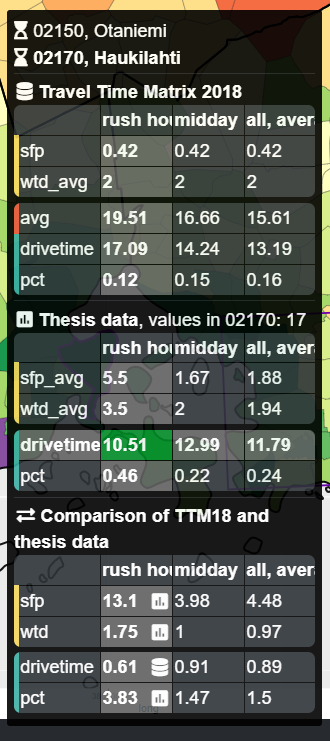
\includegraphics[width=0.33\textwidth]{images/shinyapps_comparison_detail.png}
    \caption[Comparison application data]{Close-up of a tooltip for a travel chain from 02150 Otaniemi to 02170 Haukilahti. The cell coloured green tells the user that currently visualised on map is thesis data, the travel chain without searching for parking or walking to one's destination, in rush hour traffic.}%
    \label{fig:shinyapps_comparison_detail}%
\end{figure}

\begin{figure}[H]%
    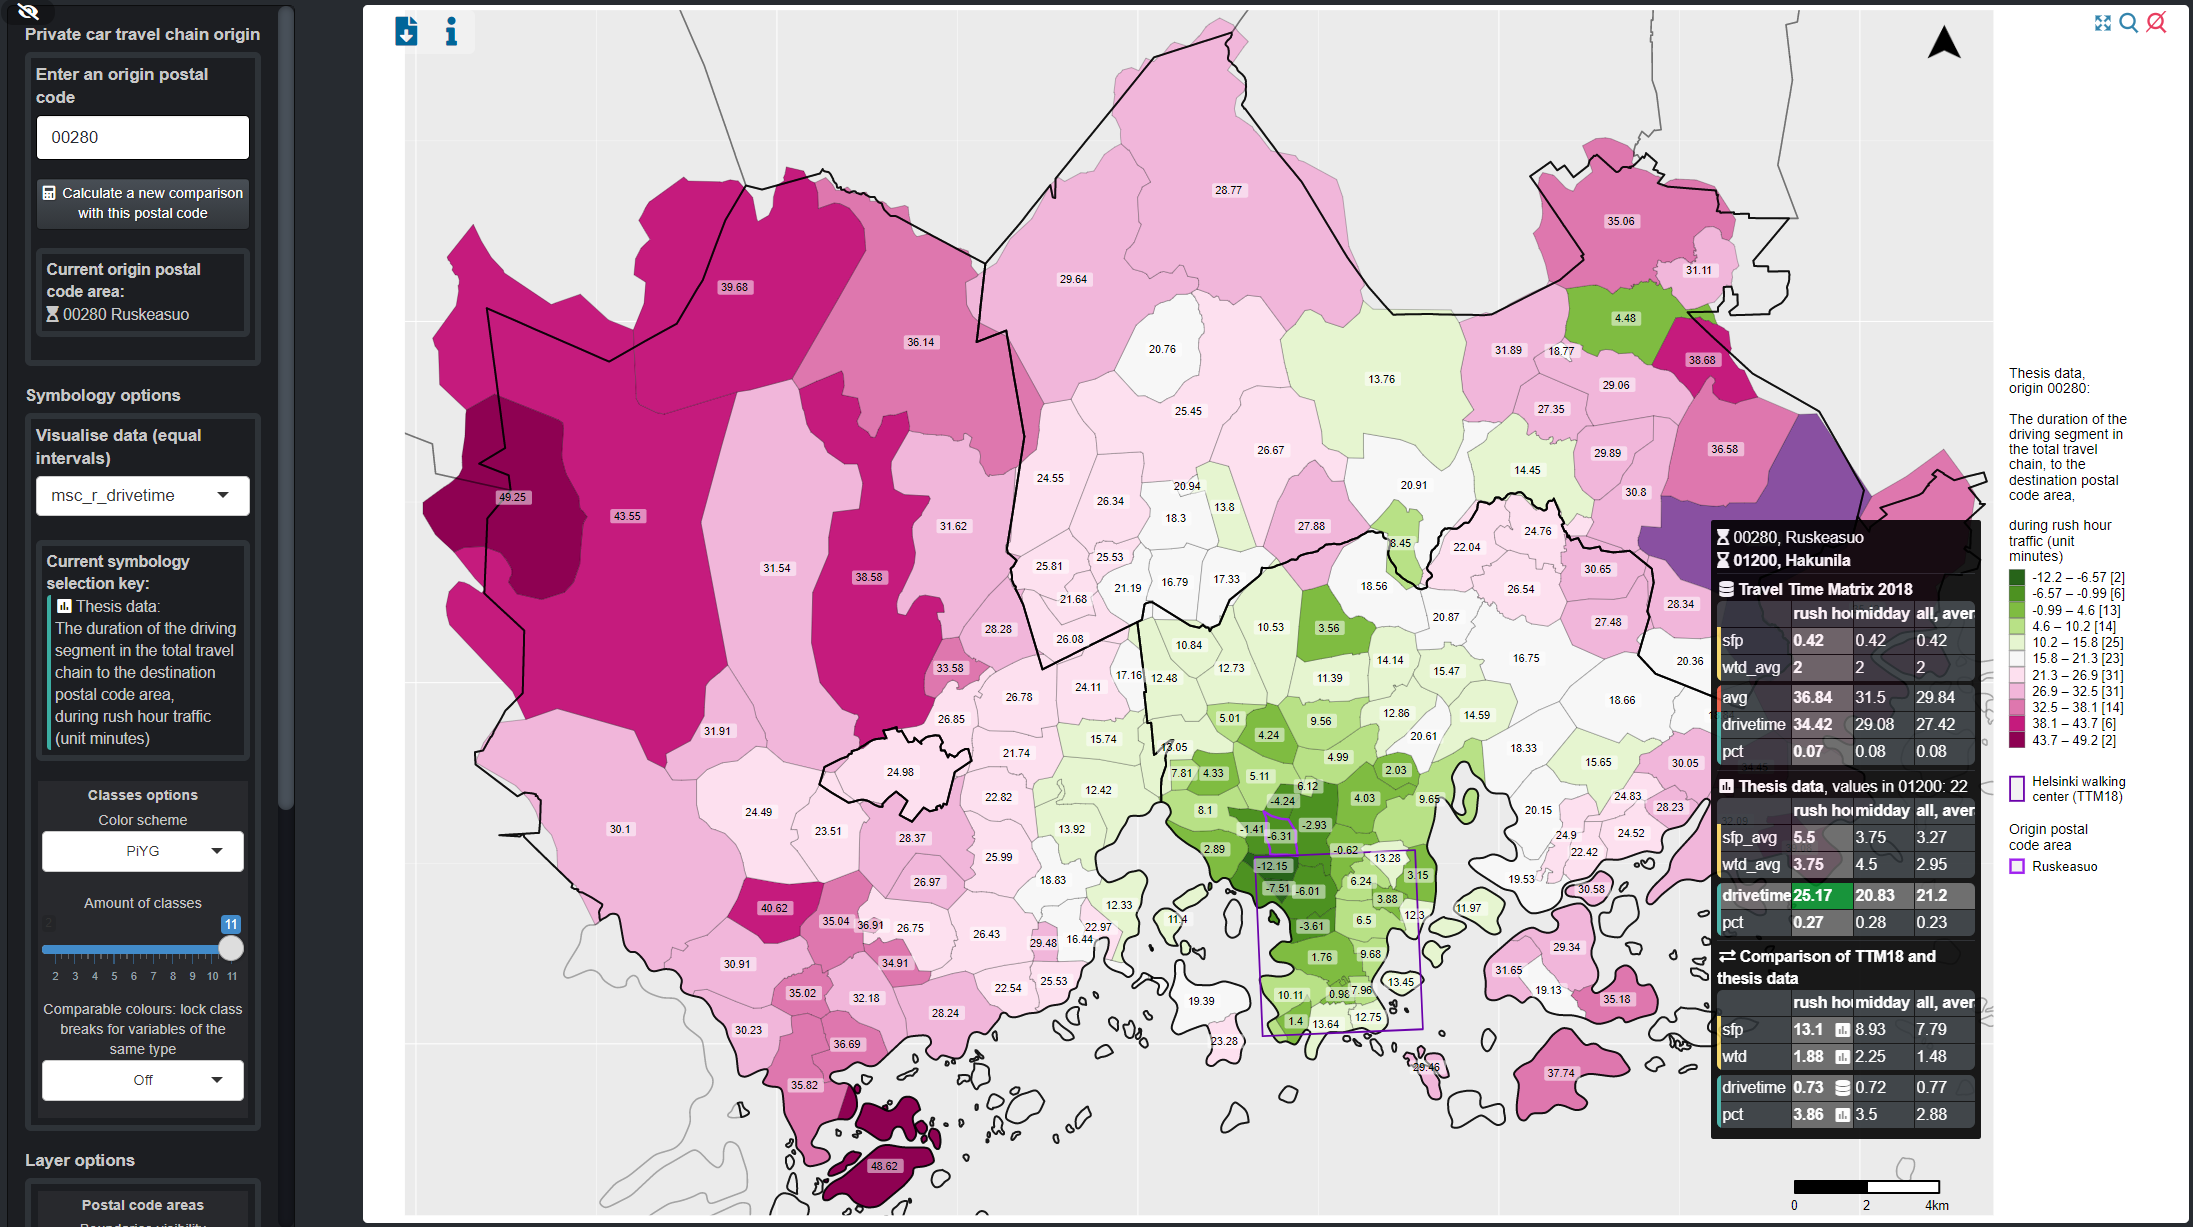
\includegraphics[width=\textwidth]{images/shinyapps_comparison.png}
    \caption[Comparison application screenshot]{Helsinki Region Travel Time Matrix 2018 and thesis survey data comparison application's shinyapps.io deployment. The cursor hovers over 01200 Hakunila with the appropriate tooltip shown.}%
    \label{fig:shinyapps_comparison}%
\end{figure}

The source code for the travel time comparison application is available at GitHub (\textcolor{blue}{\url{https://github.com/sampoves/thesis-comparison-shinyapps}}). The application may be viewed on shinyapps.io (\textcolor{blue}{\url{https://sampoves.shinyapps.io/comparison}}).
%\section{Data and methods}
\subsection{General workflow}
\justify

A selection of web applications were designed and programmed for this thesis. In this chapter the process to create these applications is presented, from the design board to a functional web application to the end stage of data processing and visualisation. Four applications are presented in this chapter: a spatial web survey for data collection, and three separate web applications for the analysis and visualisation of the survey results.

Essential data for this research was provided by Statistics Finland, the research group Digital Geography Lab of University of Helsinki, the municipalities of Helsinki Capital Region, and Finnish Environment Institute. The research area of this thesis was based on PAAVO open data by postal code area (\cite{StatisticsFinland2019a}. Data such as the CORINE Land Cover 2018 artificial surface polygons and areas of urban structure were utilised to provide additional explanatory variables in the survey data (\textcolor{red}{cite corine}; \cite{Ristimaki2017}). For the visualisation of the survey results, various data by Statistics Finland was used (\cite{StatisticsFinland2012}).

Several programming languages were used to develop the survey web application and the subsequent data processing, analysis, and visualisation applications. The survey itself was created with HTML, JavaScript and PHP, with the essential help of Leaflet, a JavaScript mapping library (\cite{Agafonkin2019}). Data processing was a shared process between Python and R. Initial processing was done in Python and the analysis and visualisation in R. In Python, the library GeoPandas was in a central role, while interactive analysis and visualisation applications were created with the library Shiny (\cite{GeoPandasDevelopers2019}, \cite{Chang2019}). The thesis itself was written with LaTeX, a document preparation system, using the online LaTeX editor Overleaf (\textcolor{red}{cite}).

Initially, the research survey strove to collect parking event data on the precise temporal and spatial resolutions of an individual parking event and its exact coordinates, respectively. This first version of the survey created with Survey123 for ArcGIS was released to a small group of people before a planned larger roll-out, but it was quickly decided that a survey of a more general spatial and temporal resolution was needed to secure enough responses. After some consideration, one was programmed from the ground up using HTML and JavaScript. In this new survey, which was rolled out in May 2019, the respondent would send data about their parking activities in a specific postal code areas in a general sense, summing up their experiences in the most recent two years. The reduction in data resolution was substantial, but would still have more spatial fidelity than the existing parking time data in Helsinki Region Travel Time Matrix 2018 (\textcolor{red}{ttmcite}).

The survey was carried out in the four municipalities of Helsinki Capital Region. An invitation to participate in the survey was spread mostly in city district and neighborhood groups in Facebook. The response collection period continued until October 2019. The survey gathered, in total, 5222 responses from 4309 unique IP addresses.

After the conclusion of the data collection phase, the survey data was processed, analysed, and visualised using Python and R programming languages. The process started with anonymisation of the IP address data, and moved on to the processing proper. The objective of the data processing in Python was to bind the survey data with a selection of open spatial data in an effort to create additional explanatory variables for analysis.

The survey result analysis and visualisation was carried out in R. Utilising Shiny, a web application framework library for R, data analysis and visualisation applications were programmed for efficient and flexible data analysis for this thesis, but also to release the survey results to the public, maintaining the mission of openness and transparency of this thesis. \textcolor{red}{mieti josko avaisi shinyappien sisältöä tähän}

The general workflow of the thesis data processing can be viewed in figure~\ref{fig:gen_workflow}.

\begin{figure}[H]
    \centering
    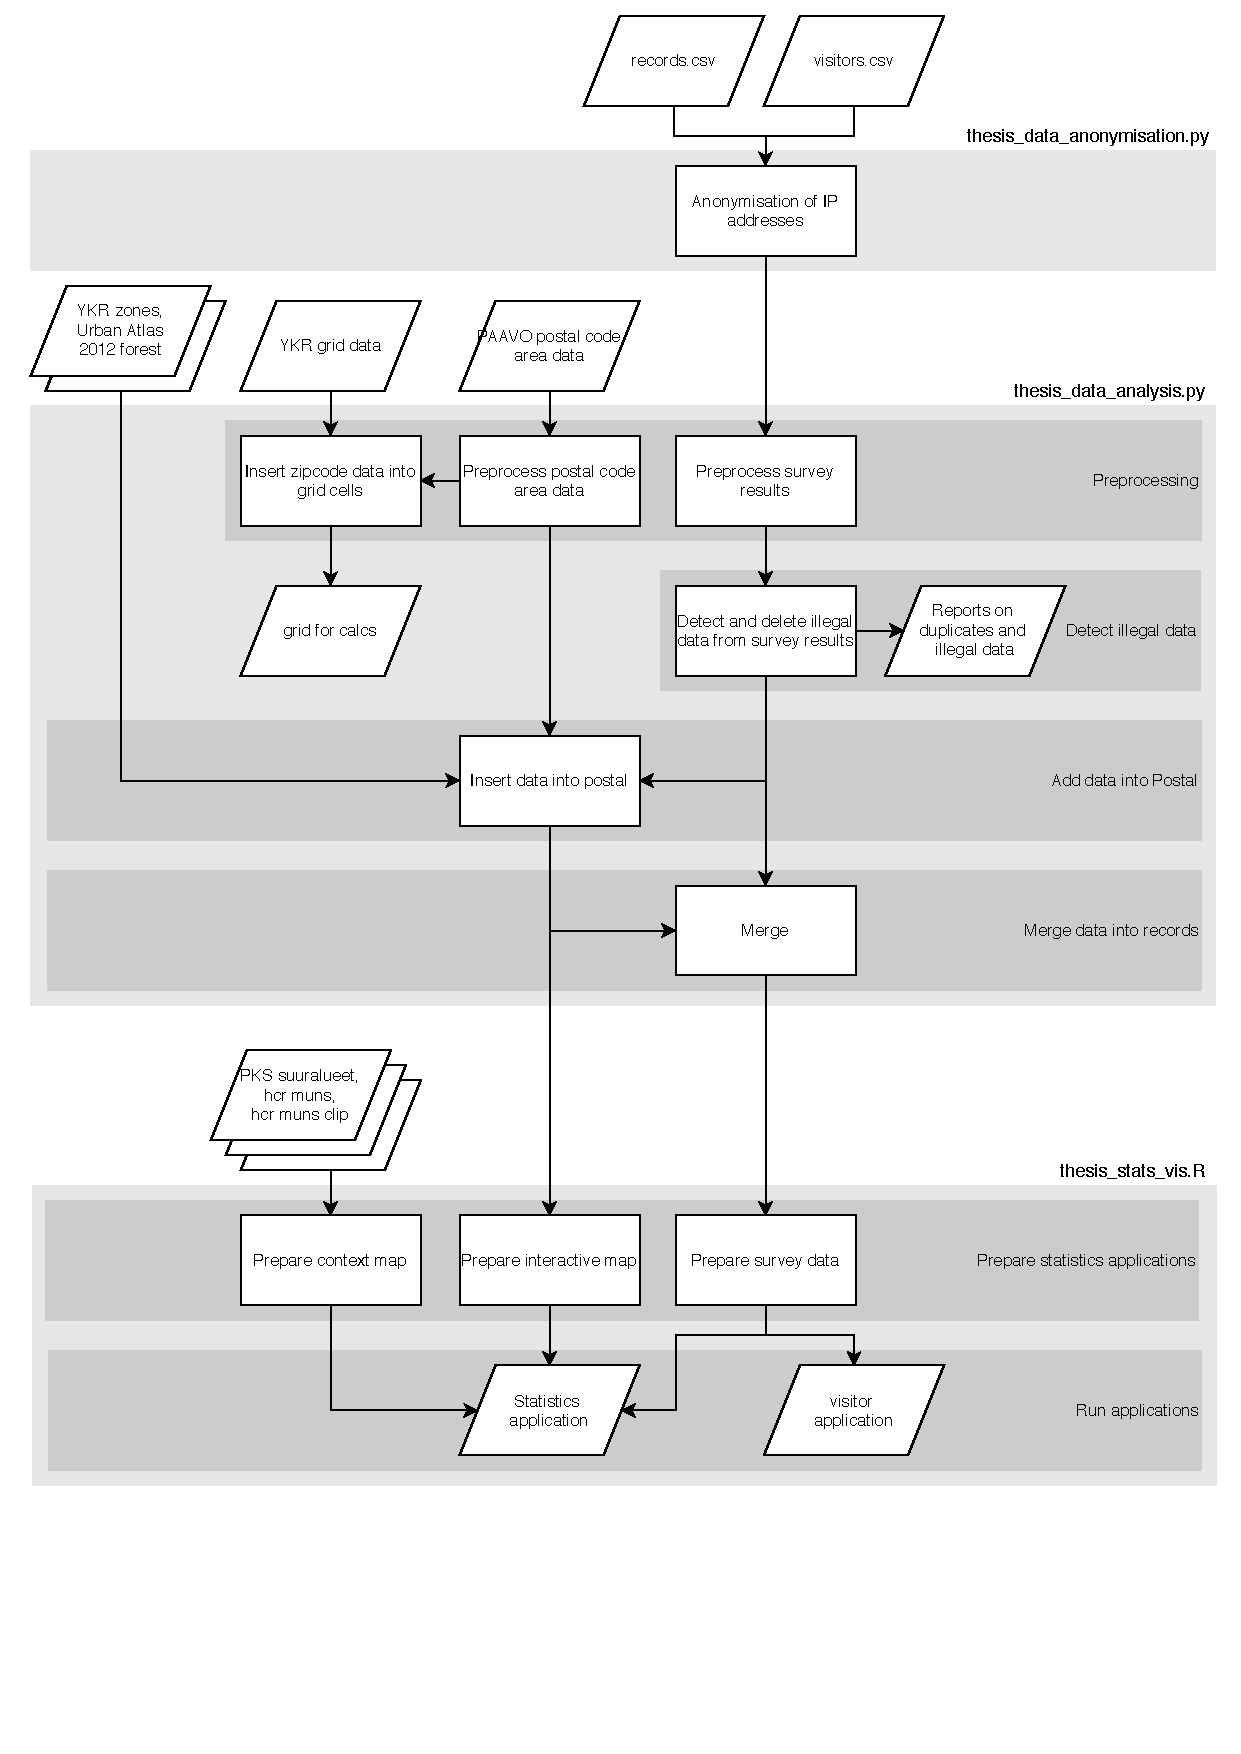
\includegraphics[trim=0.5cm 2.0cm 0.5cm 0.5cm,width=\columnwidth,scale=0.5]{thesis_workflow.pdf}
    \caption{The general workflow of the thesis survey data processing in Python and R.}
    \label{fig:gen_workflow}
\end{figure}
\pagebreak

\newpage
\subsection{Study area}
\justify
% https://www.hel.fi/hel2/Helsinginseutu/HS_tunnusluvut/liikennemaara_ja_autonomistus.pdf
% https://www.hsl.fi/sites/default/files/19_2016_auton_omistus_helsingin_seudulla.pdf
% https://www.hsl.fi/tutkimukset/muut-selvitykset
% http://pxnet2.stat.fi/PXWeb/pxweb/fi/StatFin/StatFin__lii__mkan/

\textcolor{red}{add content to this chapter} The study area of this thesis is the Helsinki Capital Region in Finland. It comprises of municipalities of Helsinki, Espoo, Vantaa and Kauniainen. The total population of the metropolitan area is 1.5 million \textcolor{red}{LÄHDE}. In practice, the whole area amalgamates as one complete functional area with boundaries of the municipalities indistinguishable at the street level. The Helsinki Capital Region faces increasing pressure to manage its traffic because \textcolor{red}{LÄHDE}. Of these four municipalities Helsinki is the hub, and considered to contain the only inner city features of the municipalities (\textcolor{red}{syke-urbanareas}). Espoo, Vantaa and Kauniainen mostly consists of suburban areas with occasional industrial areas and large shopping complexes placed throughout the area. The Helsinki Capital Region is served with a high-performance public transport system comprised of buses, train, subway, and tram in Helsinki. Recently, in 2017, the subway expanded from Helsinki to Espoo, triggering a new phase of quickly evolving cityscape in the surroundings of the new stations.

\begin{figure}[H]%
    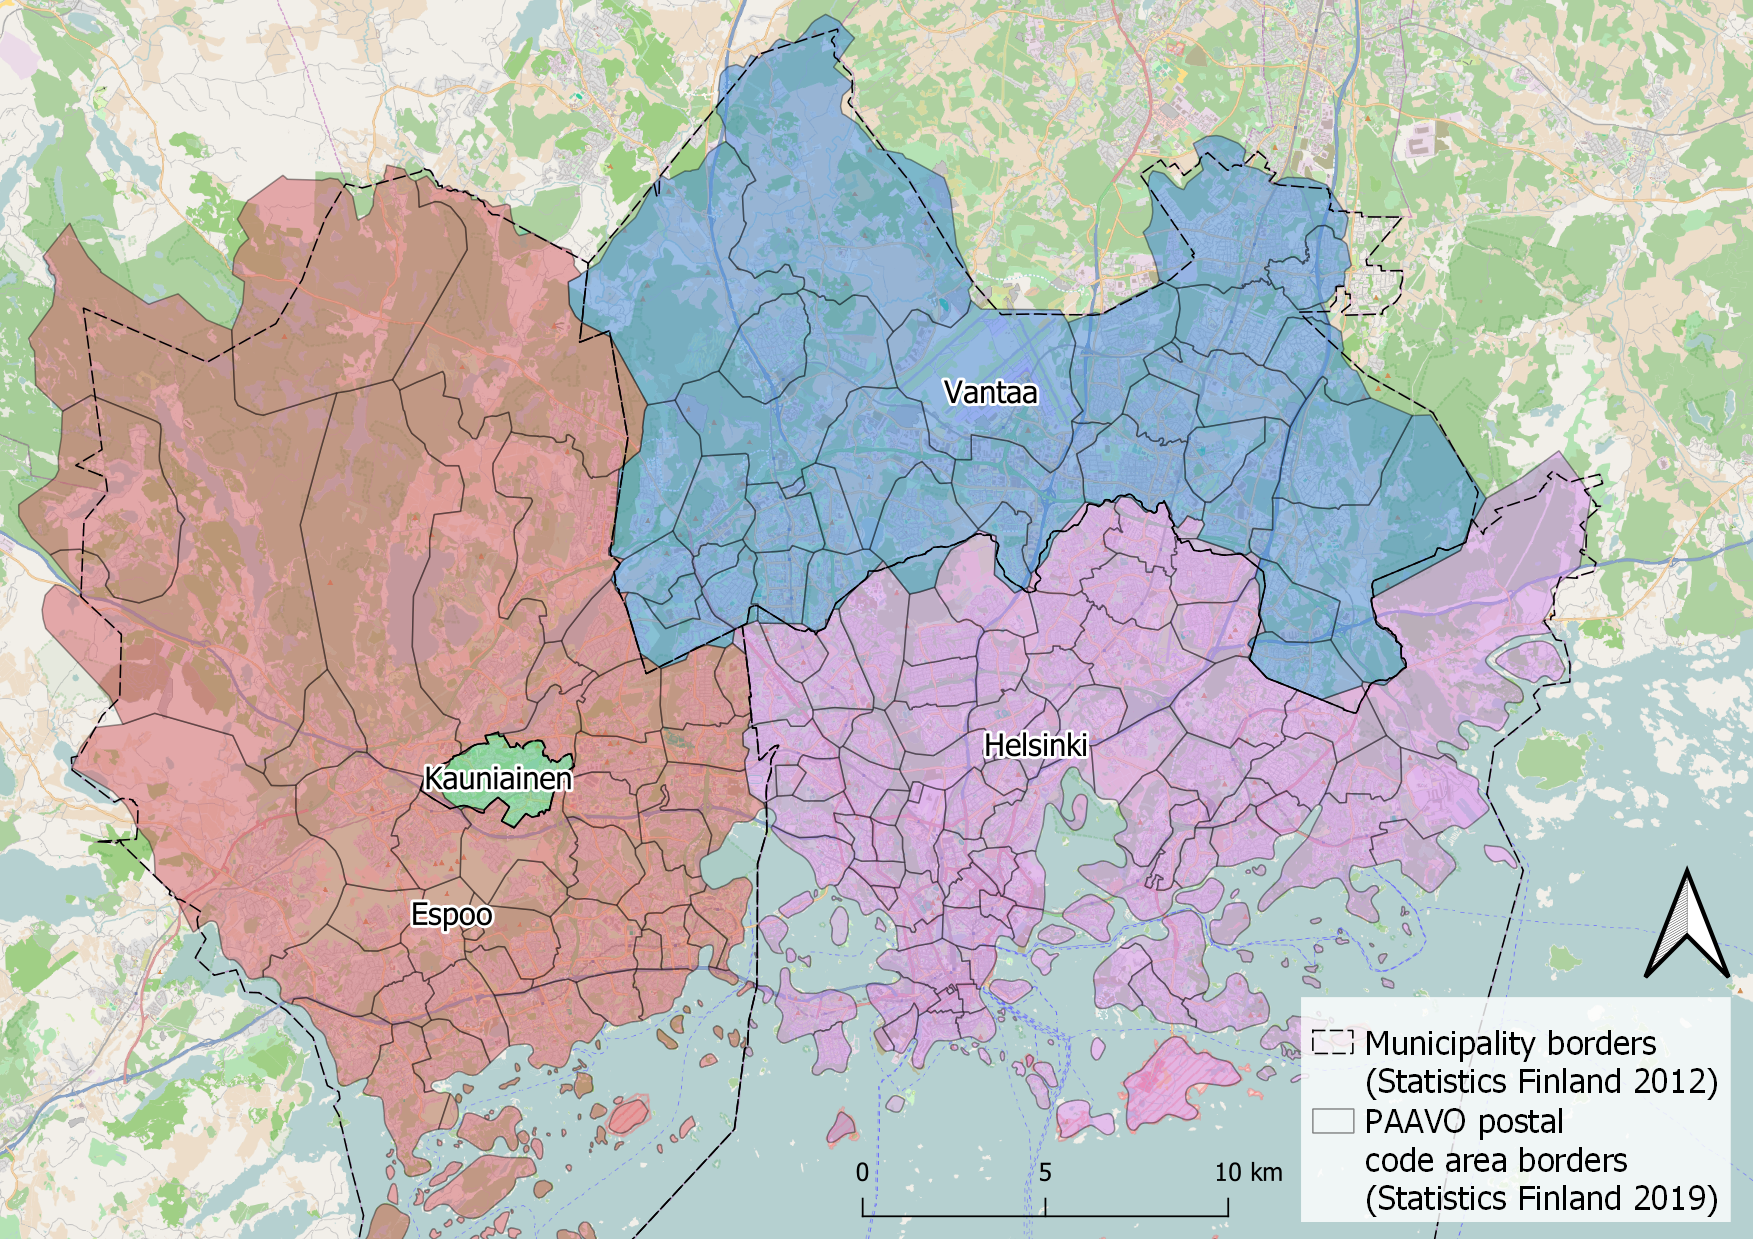
\includegraphics[width=\textwidth]{images/thesis_resarea.png}
    \caption[Research area map]{Map of the Helsinki Capital Region, the research area of this thesis. This research focuses on PAAVO postal code areas. The data has a municipality value for each postal code area (see the colouring of areas and map legend) but the areas do not completely align with the official municipality boundaries. \textcolor{red}{osmcite}}%
    \label{fig:thesis_resarea}%
\end{figure}

Despite the extensive service level of Helsinki Capital Region public transport, households especially in Espoo, Vantaa, and Kauniainen remain dependent on personal vehicles (\textcolor{red}{LÄHDE}). 

\newpage
\subsection{Data}
\justify

The foundation of this research is the dataset \textit{PAAVO -- open data by postal code area} (abbreviated \textit{postal} in this thesis) (figure~\ref{fig:paavo_resarea}). This data provides a large selection of data regarding the population of every postal code area in Finland. This includes detailed demographics and data about employment by field which follows the industrial classification TOL 2008 (\cite{Tilastokeskus2008}). However, this thesis only utilises the spatial definitions of the postal code areas, using these polygons to differentiate areas from each other in the web survey. This research makes use of the PAAVO 2018 dataset, released in January 2019.

In this thesis, the \textit{CORINE Land Cover 2018} (abbreviated \textit{CORINE}, figure~\ref{fig:datalayers}) vector format dataset is used to locate built area, or artificial surface, in the Helsinki Capital Region (\textcolor{red}{corinecite}). Provided by Finnish Environment Institute, CORINE contains polygonal data about land cover and land use for the entire nation in different hierarchy levels. In this thesis, the hierarchy level 1 value \textit{Artificial surfaces} is used. The minimum unit depicted in this dataset is 25 hectares in area or 100 meters in width. This slightly coarse data fits well with the spatially simplified nature of PAAVO postal code areas. CORINE dataset is an integration of automated satellite image interpretation and existing digital map data. \textcolor{red}{lisää taulukko siitä mitä level 1 artificial surfaces sisältää}

A main focus in this thesis was to compare the thesis survey results with \textit{Helsinki Region Travel Time Matrix 2018} (abbreviated \textit{TTM}), a dataset provided by Digital Geography Lab, a research group based in the University of Helsinki, the department of geosciences and geography (\cite{Tenkanen2018}). Their newest dataset provides travel times for public transport, private car, walking, and bicycling between all MetropAccess-YKR-grid cells (n=13231) \textcolor{red}{varmista että selitetty tätä ennen metropaccess ykr}. All travel times in this dataset were calculated using the door-to-door approach, which incorporates all parts of a journey from place A to place B into the travel time, including walking from one's home door to the car or bus stop and the time spent searching for parking. This thesis focuses on journeys made by private car.

\textit{MetropAccess-YKR-grid} (abbreviated \textit{grid}, figure~\ref{fig:datalayers}) is a spatial dataset consisting of cells with the dimensions of 250 by 250 meters (\cite{Toivonen2014a}). The dataset is used in the MetropAccess project of Digital Geography Lab and is based on the YKR data provided by Finnish Environment Institute and Statistics Finland (\cite{StatisticsFinland2020}). \textit{Grid} is a simple dataset and contains the spatial coordinates of cells and their identifiers, called the YKR ID. Using the YKR ID it is easy to connect \textit{TTM} data with the statistical data provided by Statistics Finland, allowing wide-ranging possibilities for further research.

All postal code areas in the survey results were classified with the \textit{zones of urban structures} (officially \textit{Yhdyskuntarakenteen vyöhykkeet}, abbreviated \textit{YKR zones}, figure~\ref{fig:datalayers}) (\cite{Ristimaki2017}). Utilising the same statistical grid of 250 x 250 meters as MetropAccess-YKR-grid, \textit{YKR zones} classifies grid cells to produce pedestrian, public transport, and automobile zones in and around Finland's urban regions using the theory of urban fabrics. According to this theory, these three zones developed during different times in the urban region's history (\cite{Newman2016}). In this thesis, every postal code area is assigned with a class defined in the \textit{YKR zones} based on which class has the largest presence. Adding this data into the survey results aimed to provide more possibilities to explain the hypothetical dissimilarity of survey results in different parts of the Helsinki Capital Region.

\textit{The regional division maps of Helsinki Capital Region} (officially \textit{Pääkaupunkiseudun aluejakokartat}, abbreviated \textit{subdivisions}, figure~\ref{fig:subdiv_placement}) was used in this thesis to analyse and visualise the survey results by subdivisions of Helsinki Capital Region (\cite{HelsinginEspoonVantaanjaKauniaistenmittausorganisaatiot2011}). Dividing the survey results into subdivisions would potentially give rise to local phenomena which would not be perceptible in the finest available level of spatial resolution, the postal code areas.

The dataset \textit{Regional population density 2012} (figure~\ref{fig:subdiv_placement}) was used in this thesis to visualise the boundaries of municipalities in Helsinki Capital Region (\cite{StatisticsFinland2012}). 

\begin{figure}[H]%
    \centering
    % use percentage of pagewidth with the syntax ".00\textwidth"
    \subfloat[CORINE Land Cover 2018 artificial surfaces in Kauniainen and eastern Espoo.]{{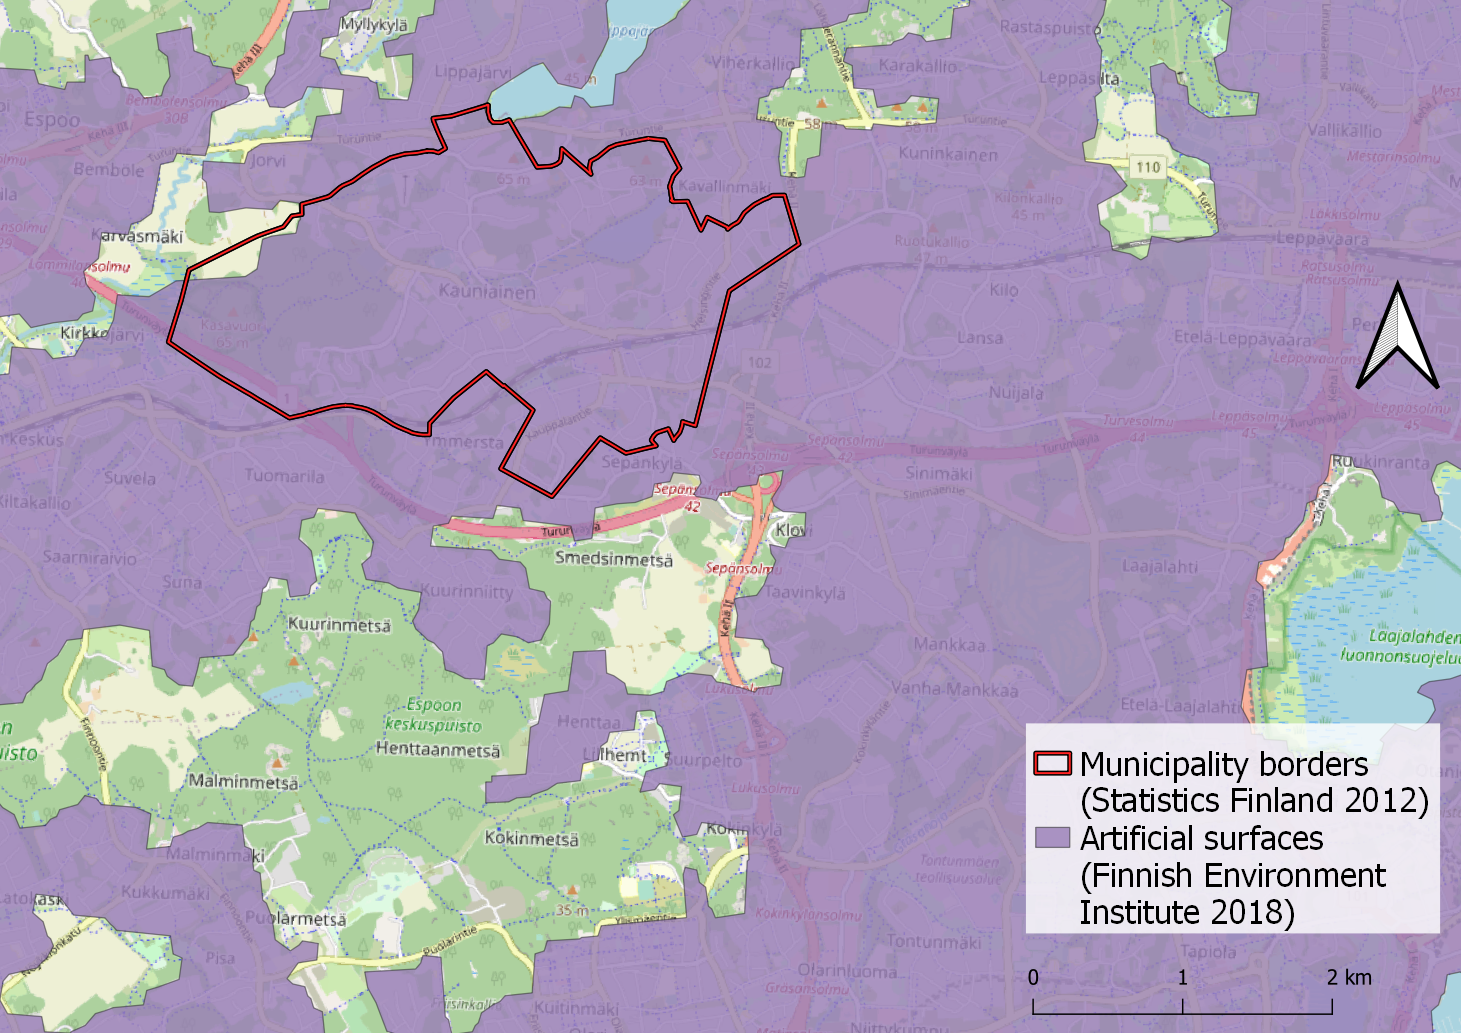
\includegraphics[width=.5\textwidth]{images/thesis_data_artificial.png} }}%
    \subfloat[Zones of urban structure in eastern Helsinki.]{{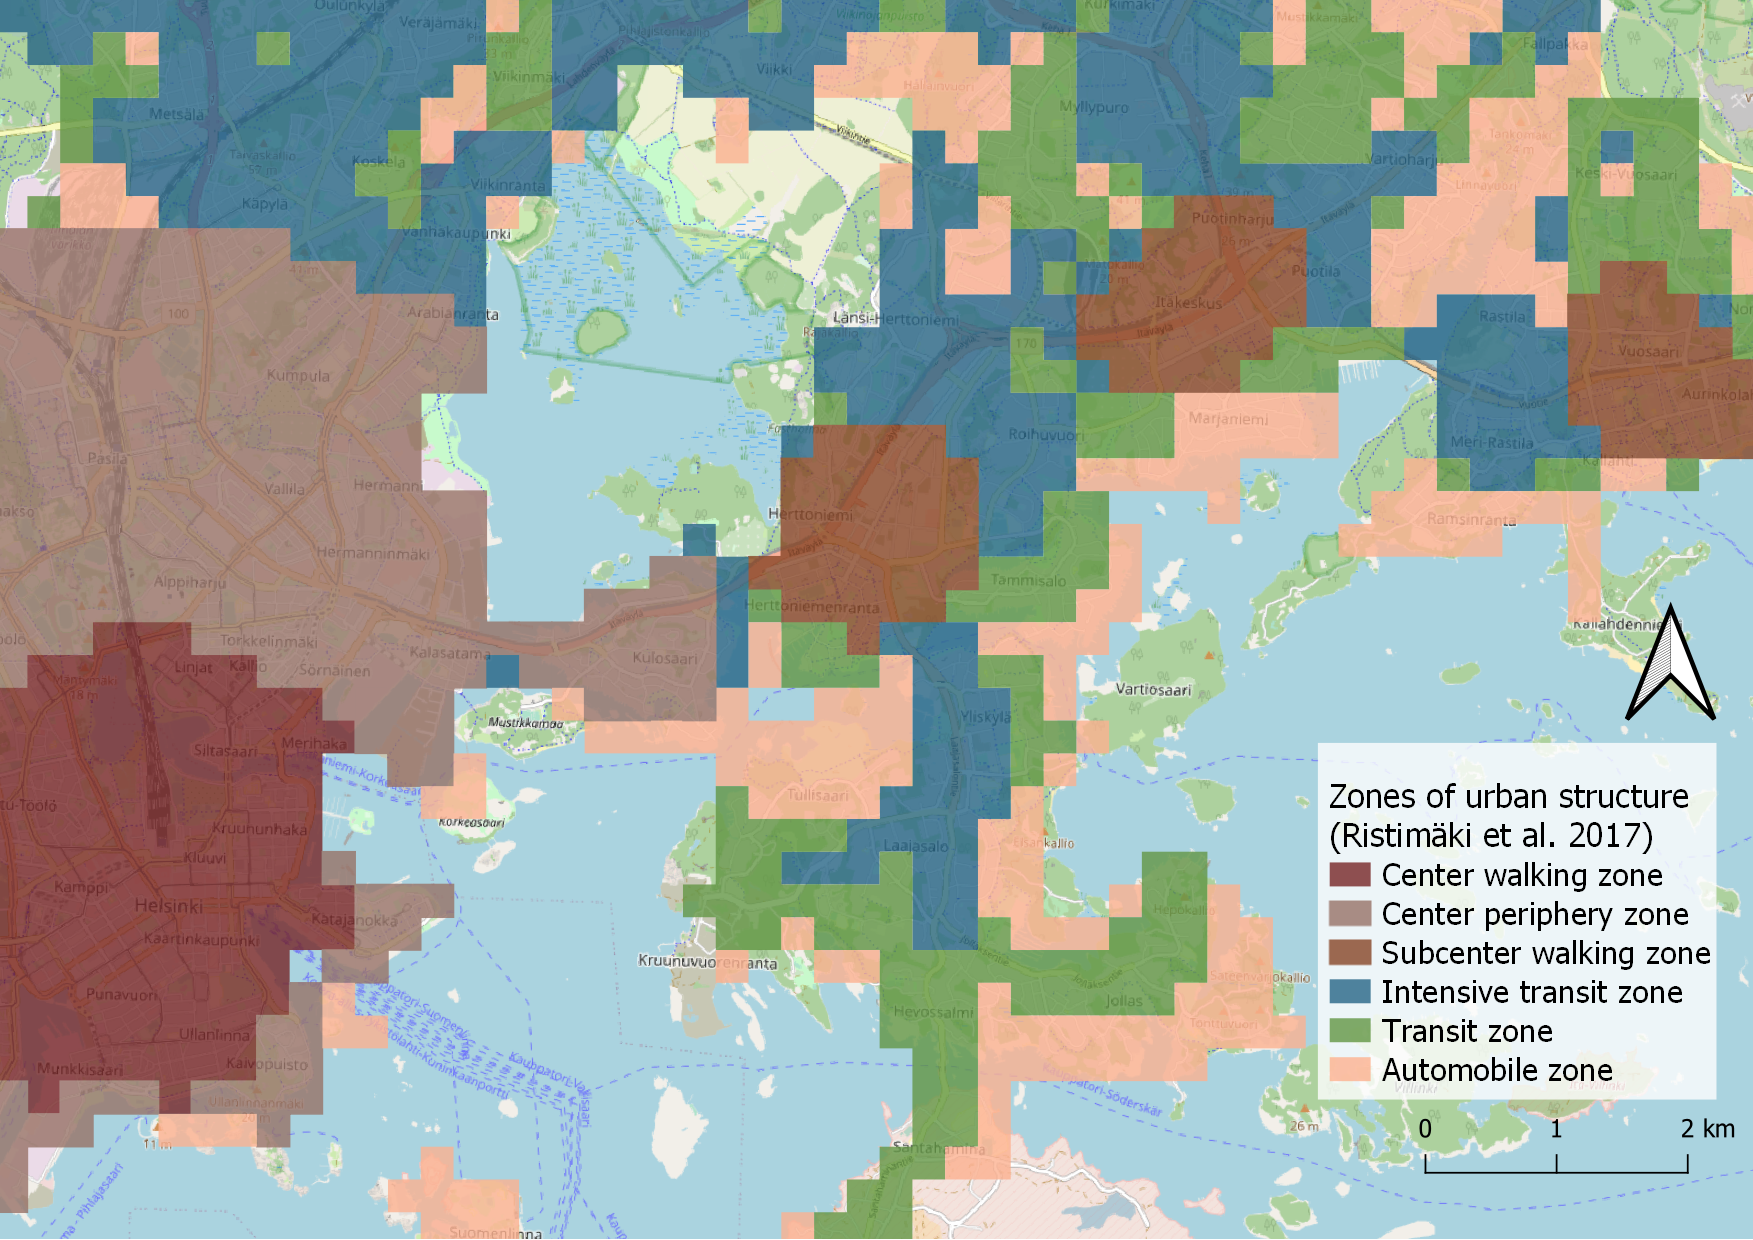
\includegraphics[width=.5\textwidth]{images/thesis_data_ykr_zones.png} }}%
    \quad
    \subfloat[MetropAccess-YKR-grid.]{{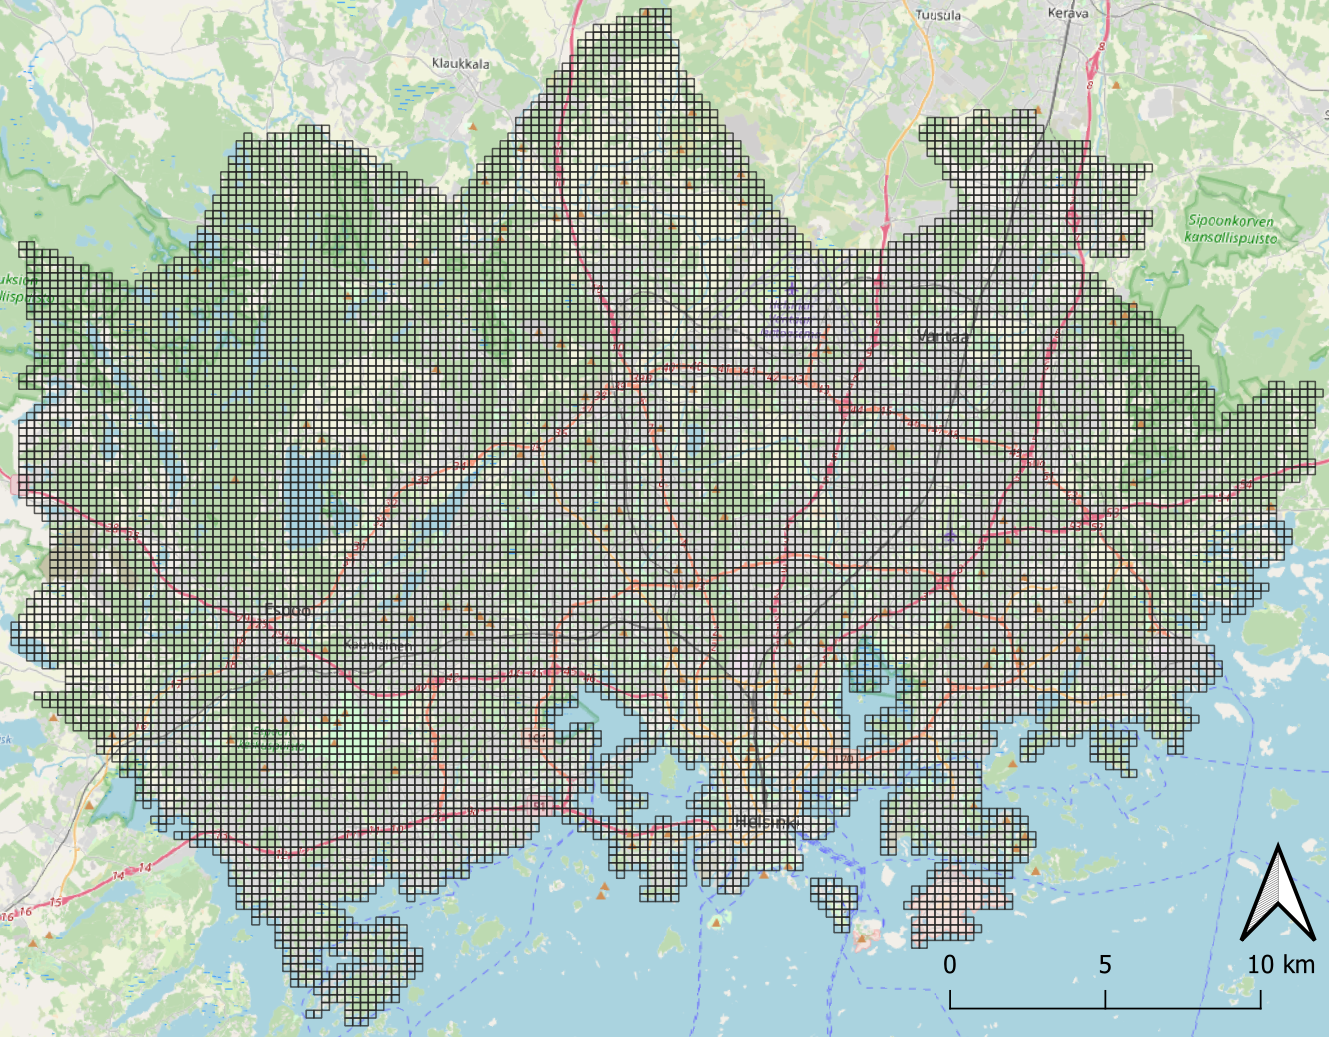
\includegraphics[width=\textwidth]{images/thesis_data_grid.png} }}%
    \caption[Spatial data]{Some of the spatial data used in the thesis. \textcolor{red}{osmcite}}%
    \label{fig:datalayers}%
\end{figure}

% hyphenrules: prevent hyphenation temporarily
\begin{hyphenrules}{nohyphenation}
    \begin{table}[H]
        \centering
        \caption[Thesis data]{Data utilised in the thesis.} 
        \label{tab:used_data}
        % use \scalebox{}{} to control table size. Note the additional curly brackets enveloping the entire tabular object
        \scalebox{0.8}
        % use \arraystretch to add whitespace between rows. \setlength\tabcolsep for columns
        {\def\arraystretch{1.5} 
        \setlength\tabcolsep{1.2ex}
        % One unit here is ">{\raggedright\arraybackslash}p{4cm}". \raggedright prevents justification of text and conveniently allows flush right or flush left, which is not possible with column command p{4cm} alone.
        \begin{tabular}{ @{} >{\raggedright\arraybackslash}p{4cm} >{\raggedright\arraybackslash}p{4cm} >{\raggedright\arraybackslash}p{4.5cm} >{\raggedright\arraybackslash}p{3.5cm} >{\raggedleft\arraybackslash}p{3.5cm} @{} }
            \toprule
            Data & Description & Purpose in thesis & Abbreviation in thesis & Citation \\
            \midrule
            CORINE land cover 2018 & Land use and land cover data in vector format & Artificial surface data & \textit{CORINE} & \textcolor{red}{cite} \\
            Helsinki Region Travel Time Matrix 2018 & Travel time and distance information for routes between all \textit{grid} cell centroids in the Capital Region of Helsinki & Use in travel time comparison calculations between \textit{TTM} and thesis survey results & \textit{TTM} & \cite{Tenkanen2018} \\
            MetropAccess-YKR-grid & Statistical grid of 250 x 250 meter cells for monitoring urban structure, Helsinki Capital Region area & Use in travel time comparison calculations between Travel Time Matrix 2018 and thesis survey results & \textit{grid} & \cite{Toivonen2014a}, \cite{StatisticsFinland2020} \\
            Paavo -- Open data by postal code area 2018 & Helsinki Capital Region postal code areas & Thesis research area and the basic unit of spatial resolution in the survey & \textit{postal} & \cite{StatisticsFinland2019a} \\
            Regional population density 2012 & Population density with municipality boundaries & Visualisation in R & \textit{hcr\_muns} & \cite{StatisticsFinland2012} \\
            Subdivisions of Helsinki Capital Region & The subdivisions of the municipalities of Helsinki Capital Region & Visualisation in R & \textit{subdivisions} & \cite{HelsinginEspoonVantaanjaKauniaistenmittausorganisaatiot2011} \\
            Zones of urban structure (Yhdyskuntarakenteen vyöhykkeet) 2017 & Delineation of urban areas based on the theory of urban fabrics & Data on spatial structure of urban areas & \textit{YKR zones} & \cite{Ristimaki2017} \\
            \bottomrule
        \end{tabular}}
    \end{table} 
\end{hyphenrules}

\newpage
\subsection{Used software}
\justify

A wide variety of software was used in the research for this thesis. The research strived for maximum openness and transparency and therefore much of the software employed in this work is free, open-source, or both. The research survey application utilised several essential web technologies such as JavaScript, HTML, CSS and PHP (table~\ref{tab:used_langs}). Using the web mapping library Leaflet, with the assistance of jQuery and other libraries, a modern and easy-to-use survey web application was created. Server-side, the programming language PHP was used to verify received data.

Data processing was carried out in Python 3.7.6 and R for Windows 3.6.3, with the initial processing done in Python and most of the analysis and visualisation in R (table~\ref{tab:used_langs}). Much of the work depended on additional software libraries available for the programming languages (table~\ref{tab:used_soft}). Python Anaconda version 2020.02 -- a distribution for Python for statistical computing -- provides the majority of the needed software libraries in the installation package, with the notable exception of GeoPandas, a library for geospatial pandas DataFrames in Python, and Shapely, a library for manipulation and analysis of planar geometric objects. In R, many libraries were used to achieve a comprehensive set of descriptive statistics. Libraries such as Shiny, ggplot2, and ggiraph formed the basis of the visualisation of the survey results.

% latex is not a programming language for the most part: https://www.quora.com/Is-LaTeX-a-programming-language
The thesis was written and typeset with LaTeX using the online LaTeX editor Overleaf. LaTeX is a document preparation system, used to create documents such as scientific articles. LaTeX adheres to the WYSIWYM (what you see is what you mean) system, as opposed to the "what you see is what you get" (WYSIWYG) system of text editors such as Microsoft Word, meaning that after establishing a set of parameters LaTeX will automatically compute the document formatting, while the user can concentrate on the document content. While LaTeX can be considered a programming language, it is more closely related to markup languages such as HTML (\textcolor{red}{cite}). In this LaTeX document, the LaTeX distribution TeX Live 2019 was used. Overleaf supports GitHub integration and as a result the complete thesis is available for viewing in the GitHub repository \textcolor{blue}{\url{https://github.com/sampoves/Masters-2020}} alongside with its entire development history. Additionally, the template of this thesis is provided at \textcolor{blue}{githublink, repo not started}.

In addition to the aforementioned technologies, the flowcharts in this thesis were created with the web application diagrams.net (\textcolor{red}{cite}). Most of the map visualisations of this thesis were made using the geographic information system application QGIS version 3.12.2.

% Consider! Removing \raggedright and hyphenrules will enable nice even table cells. Could be worth it to look into
\begin{hyphenrules}{nohyphenation}
    \begin{table}[H]
        \centering
        \caption[Thesis programming languages]{Programming languages, essential technologies, and \glspl{ide} utilised in the thesis, grouped by the function in this thesis.} 
        \label{tab:used_langs}
        \def\arraystretch{1.4}
        \setlength\tabcolsep{1.2ex}
        \begin{tabular}{ @{} >{\raggedright\arraybackslash}p{3cm} >{\raggedright\arraybackslash}p{4.5cm} >{\raggedright\arraybackslash}p{3.5cm} >{\raggedleft\arraybackslash}p{3.5cm} @{} }
            \toprule
            Programming language and \gls{ide} & Description & Purpose in thesis & Citation \\
            \midrule
            JavaScript, HTML, CSS (NetBeans 8.2.0) & Essential web technologies & Research survey programming, analysis and visualisation application programming & \cite{WHATWG2020}, \cite{W3C2020}, \cite{ECMA2019}, \cite{ApacheSoftwareFoundation2016} \\
            Python 3.7.6, Anaconda 2020.02 (Spyder 4.0.1) & Anaconda is a Python distribution for scientific computing & Survey data processing & \cite{Python3Reference}, \cite{AnacondaInc.2020}, \cite{SpyderProjectContributors2020} \\
            R for Windows 3.6.3 (RStudio 1.2.5033) & Programming language environment for statistical computing & Survey data analysis and visualisation & \cite{RCoreTeam2020}, \cite{RStudioTeam2015} \\
            LaTeX (Overleaf) & Document preparation system & Thesis formatting, structure, and writing & \textcolor{red}{latexcite, overleafcite} \\
            \bottomrule
        \end{tabular}
    \end{table} 
\end{hyphenrules}

\begin{hyphenrules}{nohyphenation}
    \begin{table}[H]
        \centering
        \caption[Essential software packages in thesis]{Essential software libraries used in the thesis. The complete list of libraries can be viewed in \textcolor{red}{appendix number something}.} 
        \label{tab:used_soft}
        \def\arraystretch{1.2}
        \setlength\tabcolsep{1.2ex}
        \begin{tabular}{ @{} >{\raggedright\arraybackslash}p{2.5cm} >{\raggedright\arraybackslash}p{3cm} >{\raggedright\arraybackslash}p{4cm} >{\raggedleft\arraybackslash}p{3cm} @{} }
            \toprule
            Programming language & Software package & Description & Citation \\
            \midrule
            % NB, manual positioning of the multirow label
            \multirow{3}{*}[-5ex]{JavaScript} & Leaflet 1.4.0 & Web mapping library for the research survey & \cite{Agafonkin2019} \\
            & jQuery 3.4.1 & Simplification of HTML DOM traversal and other features & \textcolor{red}{cite} \\
            & Font Awesome 5.13.0 & Font and icon collection & \textcolor{red}{cite} \\
            \greyrule
            \multirow{4}{*}[-6.5ex]{Python} & pandas 1.0.1 & Data analysis and manipulation & \cite{McKinney2011a} \\
            & GeoPandas 0.5.0 & Geographic data operations & \cite{GeoPandasDevelopers2019} \\
            & Shapely 1.6.4.post1 & Geometric objects, predicates, and operations & \cite{Gillies2019} \\
            & rtree 0.8.3 & Spatial indexing & \cite{Gillies2014} \\
            \greyrule
            \multirow{4}{*}[-7.0ex]{R} & Shiny 1.4.0.2 & Web application framework for R & \cite{Chang2019} \\
            & ggplot2 3.3.0 & Data visualisation & \cite{Wickham2016} \\
            & ggiraph 0.7.0 & Interactive ggplot2 graphics & \cite{Gohel2019} \\
            & dygraphs 1.1.1.6 & Interactive time series charting & \cite{Vanderkam2018} \\
            & fst 0.9.2 & High-performance writing and loading of data & \textcolor{red}{cite} \\
            \bottomrule
        \end{tabular}
    \end{table} 
\end{hyphenrules}

\newpage
\subsection{Methods}
\subsubsection{Considering survey development options}
\justify

To collect the areal parking data, the study required an interactive survey which respondents could use to submit their parking habits in a spatial fashion. To attract a largest possible number of submissions, the survey also needed to be of modern design, easy to use and its purpose easy to understand. The survey would have to be clear-cut, effortless to internalise and short in length as to prevent users getting frustrated and leaving before submitting answers. Design-wise, the spatial resolution of the survey was in question. The particular concern was that in the case of insufficient amount of answers, what kind of area delineation would be at the same time detailed enough but also streamlined enough to realistically reach results of good quality? This chapter strives to describe the process that would lead to the implemented web survey to accentuate the challenges this kind of research entail.

Once the consideration into options to produce the survey for this study had started, it quickly became apparent that there were few alternatives available and even fewer free, sufficiently customisable alternatives. Out of the proprietary options, Maptionnaire by the Finnish company Mapita was considered. They offer tailored map survey products with discounts for students. In return for the fee, a subscriber receives a time window in which to carry out their survey accompanied with tailored features and customer support -- the extent of features and support is determined by the price plan. The offered price was considered too steep for the thesis and Maptionnaire was passed on. 

Next Survey123 for ArcGIS was evaluated. An Esri operated service, Survey123 is used to create and analyse form based surveys (\cite{Esri}). It is included in the contract between University of Helsinki and Esri and thus was free to use for the study. One can quickly design a survey at the Survey123 website and share it immediately to respondents. Alternatively, the service is available as a desktop client, the Survey123 Connect, where Survey123 offers a wider range of possibilities for customisation with its adherence to the XLSForm standard. XLSForm is a standard to make authoring forms in Excel easier. With the customisability of XLSForm, users can design Survey123 surveys to the dot while employing the support for Excel style scripting for complex survey behaviour (figure~\ref{fig:survey123_xlsform}). Furthermore, Survey123 provides online tools for collaboration, analysis, and data viewing with many options for exporting the collected data.

\begin{figure}[H]%
    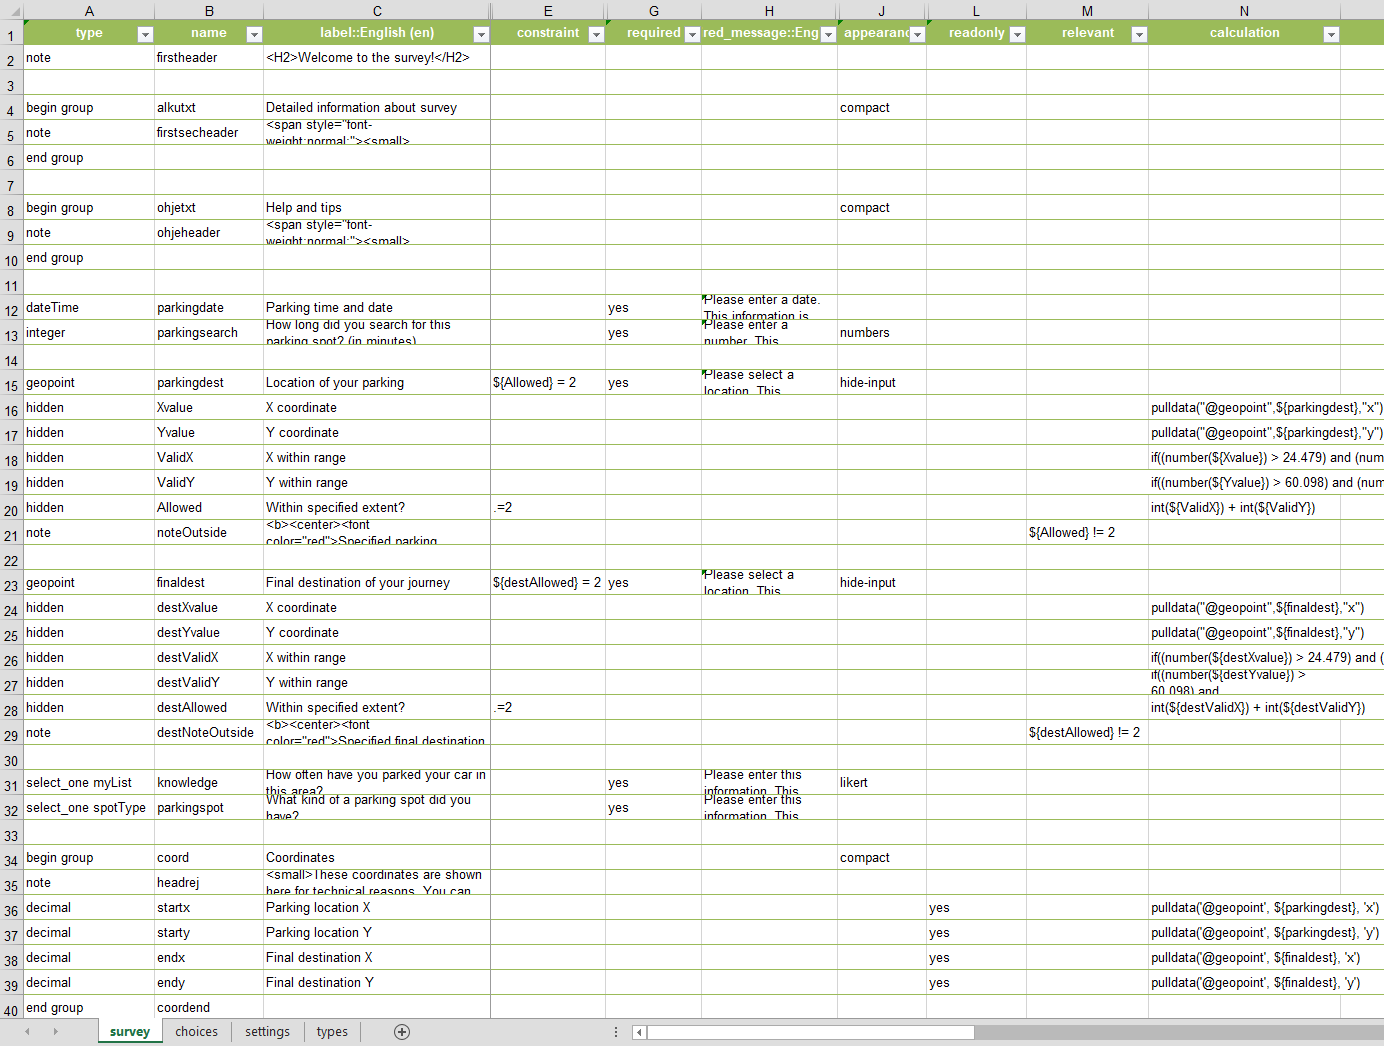
\includegraphics[width=\textwidth]{images/survey123_xlsform.png}
    \caption[Survey123 XLSForm view]{Survey123 XLSForm view in Microsoft Excel. Some parameter columns here are hidden to provide a view to the essential inner workings of the Survey123 form.}%
    \label{fig:survey123_xlsform}%
\end{figure}

% \ref{}: tilde (~) indicates a non-breaking space
In January 2019, the parking survey developed with Survey123 was deployed to friends and family, with a large scale marketing push on social media platforms planned for later. At its core, this survey asked respondents for specific parking events in Helsinki Capital Region they had had (figure~\ref{fig:survey123}). Respondents would pick an exact location on a map view for the location of their parked car and separately on a second map view the location of their final destination. In addition, respondents would fill the date and time of this parking event, how long it took for them to find a parking spot, how often they had parked to that area, and what kind of a parking spot they had taken. Respondents were asked repeat this process as many times as they had the will to do so.

The Survey123 survey was designed to reach the same spatial resolution as Travel Time Matrix 2018 with its MetropAccess-YKR-grid (grid cell 250 x 250 meters). Using exact coordinates of parkings and final destinations, it would have been possible to allocate each event to possibly two different MetropAccess-YKR-grid cell codes, reaching excellent spatial resolution. As MetropAccess-YKR-grid contains 13 231 grid cells, there was not enough resources for this master's thesis research survey to accumulate events for every grid cell, or even for most grid cells. If the data gathering campaign would have ended with insufficient amount of parking events, the backup plan was to employ an interpolation algorithm to generate approximate boundaries for the hypothetically varying parking times in Helsinki Capital Region. It was also considered that the exact coordinates of the parking events could be generalised to other boundaries, such as administrative areas like municipality subdivisions or postal code areas \textcolor{red}{explain why this was not done}. 

% utilises package subfig
\begin{figure}[H]%
    \centering
    \subfloat[Survey introduction and the date and time for the parking event.]{{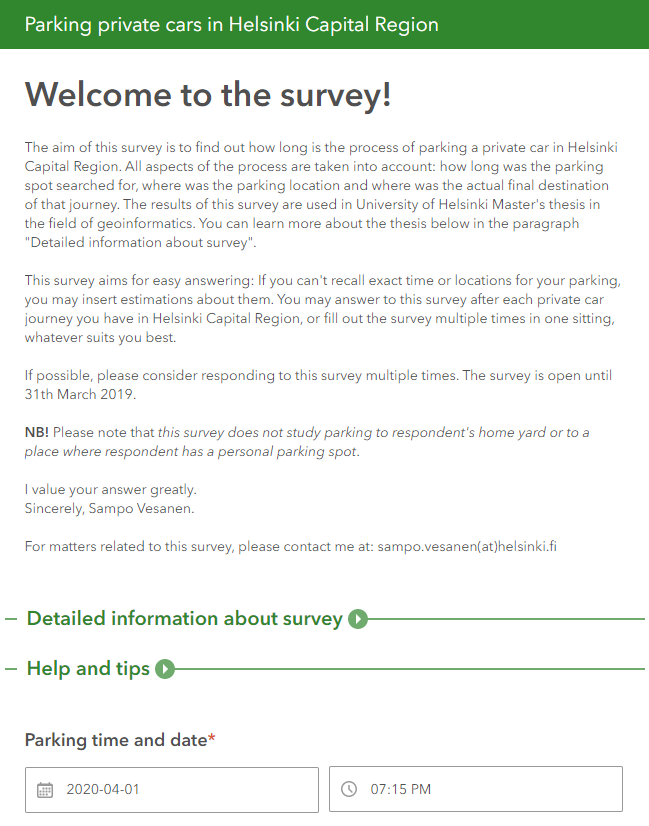
\includegraphics[width=5.5cm]{survey123_1.png} }}%
    \subfloat[Map panels for the parking location and the final destination.]{{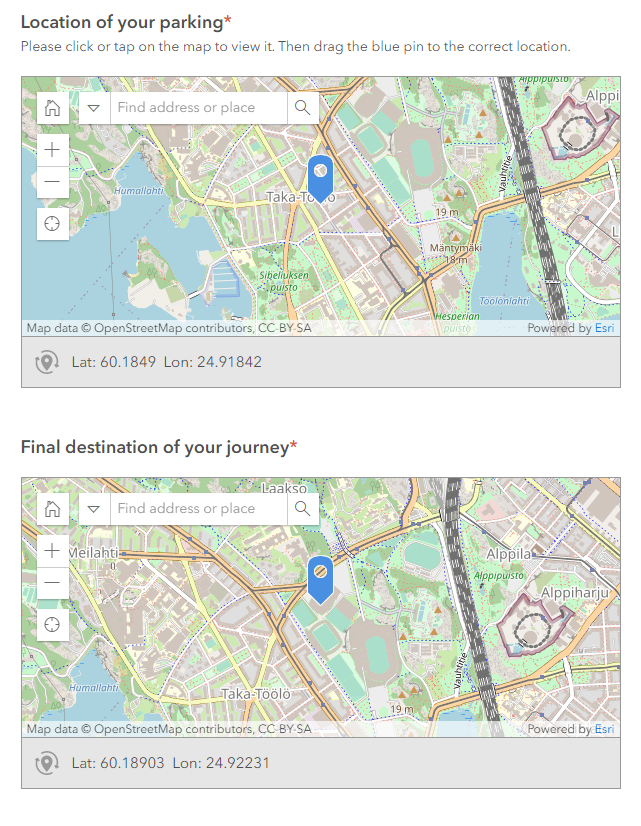
\includegraphics[width=5.5cm]{survey123_2.png} }}%
    \subfloat[Final questions of the survey.]{{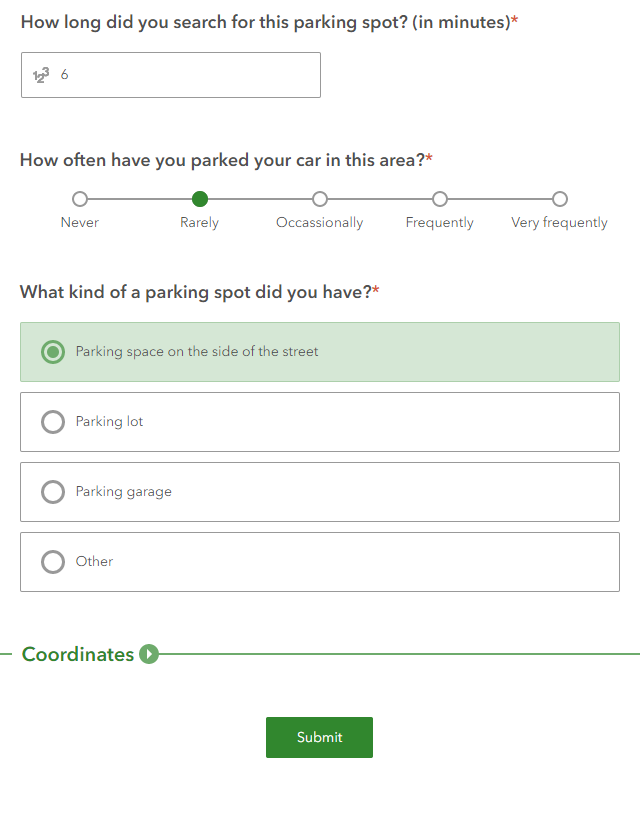
\includegraphics[width=5.5cm]{survey123_3.png} }}%
    \caption[The unused parking survey created with Survey123]{An example parking event entered into the parking research survey made with Survey123 Connect.}%
    \label{fig:survey123}%
\end{figure}

The survey was released even after Survey123 had proved itself unwieldly for the purposes of this research. The software was difficult to use because of an assortment of inconvenient design choices, unfinished functionality and a helping of software bugs. It was not possible, for example, to have respondents enter multiple parking events at once in a full screen map view. They would have to create a single parking event, send it, and then reload the survey to start from the beginning -- something a majority of prospective respondents would not have the patience for. Survey123 Connect version available at the time, 3.1.126, did not allow customisation of the post-submission message and therefore it would not be possible to efficiently direct respondents back to the form. In addition, recording coordinates from two map views was only possible through a bypass. The coordinates of the final destination would have to be printed on the form (hence the section "Coordinates" on the form in figure~\ref{fig:survey123}) and then these second set of coordinates could be saved into the survey data table in string format. The technical limitations of Survey123 as a spatial survey was witnessed also in the fact that it was not possible to add custom polygons on top of the map views. It was therefore impossible to delineate the research area for the respondents and accurately detect attempts to add parking events outside of Helsinki Capital Region.

The functionality of the released form was not reliable on the most popular web browsers such as Google Chrome and Apple Safari. Survey123 supported multi-language strings but it proved problematic to ensure that the form would open in the system language of most respondents, Finnish. In addition to this, the field for entering the specific time for the parking event was restricted to the 12 hour clock preferred in the US -- a system my target group would frown upon. To make matters worse, at that time there was a long persisting bug in Survey123 which produced unexpected behaviour, in some cases, with the use of "constraint", the parameter that controls which entered values are deemed illegal and which are not (\cite{GeoNet-TheEsriCommunity2018}). If any type of constraint statement was added, the finalised form would always claim that the related question input was invalid. The parameter would have to be left empty and therefore it was not possible to automatically prevent insertion of parking events happening in the future and excessively long times for searching for parking, reducing the quality of the survey data and making the survey form more confusing for the respondent.

\begin{figure}[H]%
    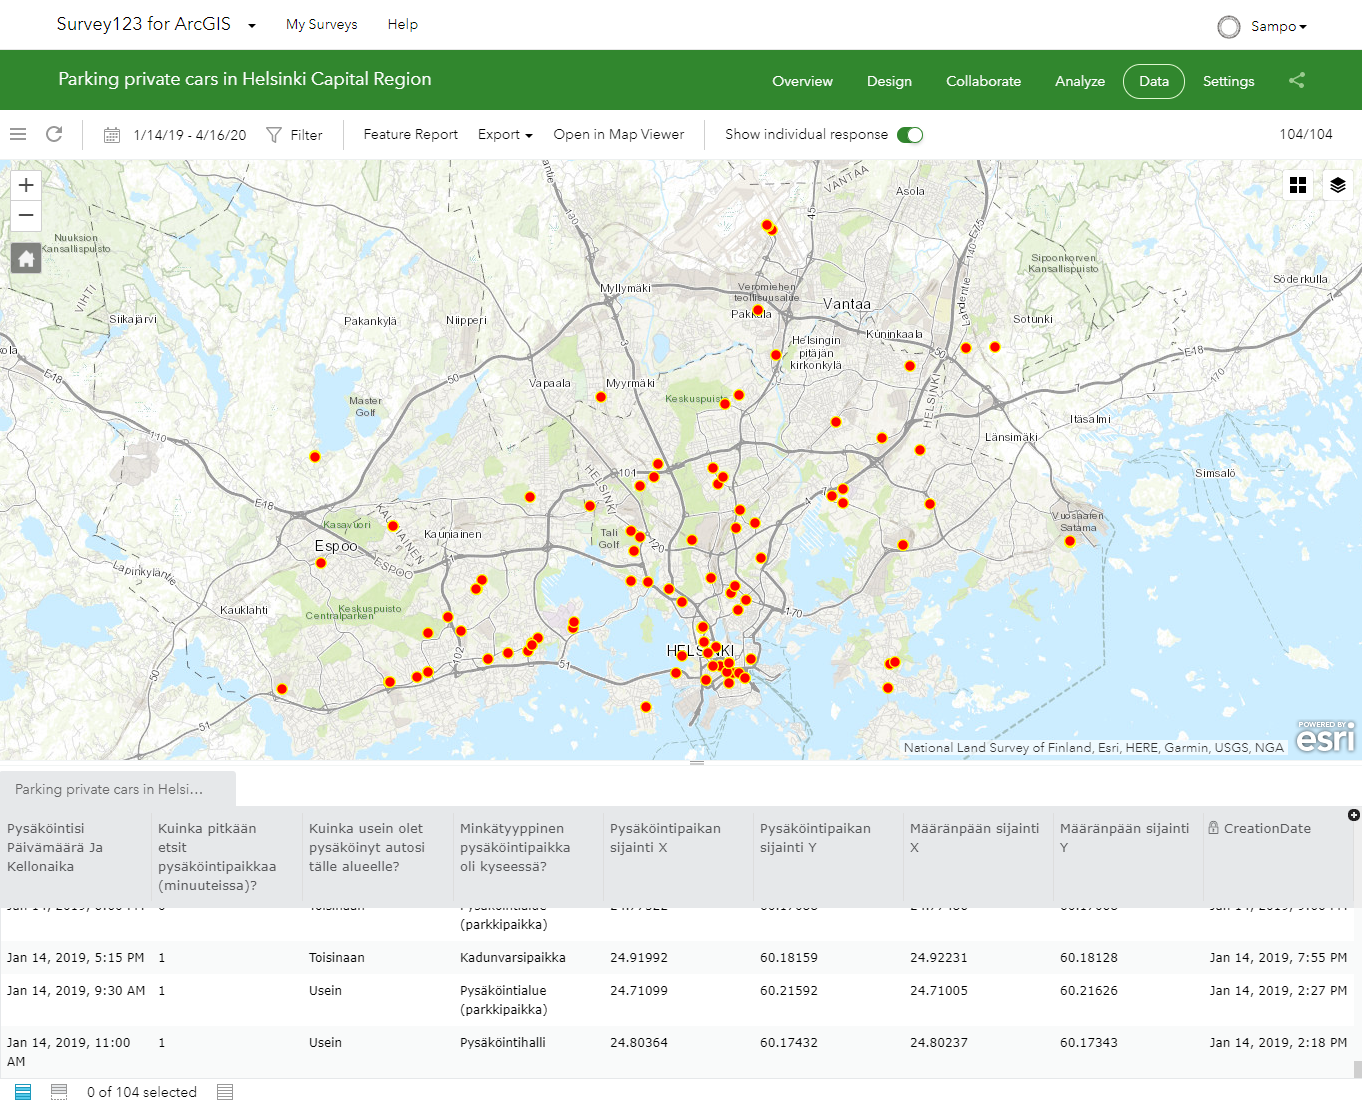
\includegraphics[width=\textwidth]{images/survey123_dataview.png}
    \caption[Survey123 data tab]{Survey123 for ArcGIS, "data" tab view in the application website. The research survey made with Survey123 received in total 104 parking events. The red dots are the final destinations of each parking event.}%
    \label{fig:survey123_dataview}%
\end{figure}

Despite the many technical incertainties of Survey123, the survey gathered more than one hundred parking events in one month (figure~\ref{fig:survey123_dataview}). This amount was achieved for the most part without advertising. Soon after the publication of the Survey123 parking survey it was decided, however, that the required spatial resolution for this research would need to be lower than exact points in an attempt to gather more responses from the entire research area. An additional deciding factor was the fact that with Survey123 respondents could not send multiple parking events with one survey session, making the form unwieldy and outdated in its rigid structure. It was argued that a more general scale would still be accurate enough to provide good data and a more generalised scale would make the survey easier to answer to and a more pleasant experience for the respondent. Postal code areas were deemed an acceptable compromise in spatial accuracy.

After careful consideration, it was decided that the survey for this thesis would have to be programmed from the ground up.

\subsubsection{Programming the parking survey}
\justify
To achieve maximum transparency and repeatability for this research, in addition to freedom in survey content and appearance, a survey web application was programmed from the ground up utilising HTML, JavaScript and PHP. The survey and its supporting infrastructure was installed on a virtual machine in CSC's -- the state owned ICT solutions company -- Taito supercluster. CSC offers virtual machines in several different hardware configurations, or flavors. The virtual machine flavor picked for this survey was \textit{standard.medium}, a flavor with 3.9 \gls{GB} \gls{RAM}, three virtual \gls{CPU}s and 80 GB of disk space. Running on the Linux distribution Ubuntu version 16.04, the backbone of the survey ecosystem was a LAMP stack, a software bundle which incorporates the Linux operating system, Apache web server software, \gls{mysql} relational database management system and the PHP programming language environment for server-side scripting. The public component of the survey is the front-end, the only component of the survey system a respondent would interact with (figure~\ref{fig:js_survey_welcome}). One may use additional software in a LAMP stack for extended functionality or can replace some of the components with a wide array of alternatives. This thesis utilises the components described in the table~\ref{tab:survey_components}.

\begin{hyphenrules}{nohyphenation}
    \begin{table}[H]
        \centering
        \def\arraystretch{1.2}
        \setlength\tabcolsep{1.2ex}
        \caption{Survey web application components} 
        \label{tab:survey_components}
        \begin{tabular}{ @{} >{\raggedright\arraybackslash}p{3cm} >{\raggedright\arraybackslash}p{3cm} >{\raggedright\arraybackslash}p{5.5cm} @{} }
            \toprule
            Component & Version & Description \\
            \midrule
            Ubuntu & 16.04.6 & Linux distribution, operating system for the virtual machine \\
            Apache HTTP Server & 2.4.18-2ubuntu3.9 & Web server software, manage website requests and responses \\
            MySQL & 5.7.25-0ubuntu0.16.04.2 & Relational database management system, survey database operations \\
            PHP & 7.0.33-0ubuntu0.16.04.1 & Programming language, used for server side scripting \\
            Parking survey front-end & 16.5.2019 & Survey visible to user, graphical user interface \\        
            \bottomrule
        \end{tabular}
    \end{table}
\end{hyphenrules}

Setting up the virtual machine for the use of the survey was a process of a few stages. The LAMP stack was installed on the fresh virtual machine with the command \code{sudo apt install lamp-server\^}. After the successful installation the MySQL tables were formed and relevant users created. The last step before a fully functioning web server was using root access to give the survey components permission to access relevant system directories. The parking survey's GitHub repository (\textcolor{blue}{\url{https://github.com/sampoves/parking-in-helsinki-region}}) may be viewed for the full step-by-step install procedure used to set up the web server for this thesis.

\begin{figure}[H]%
    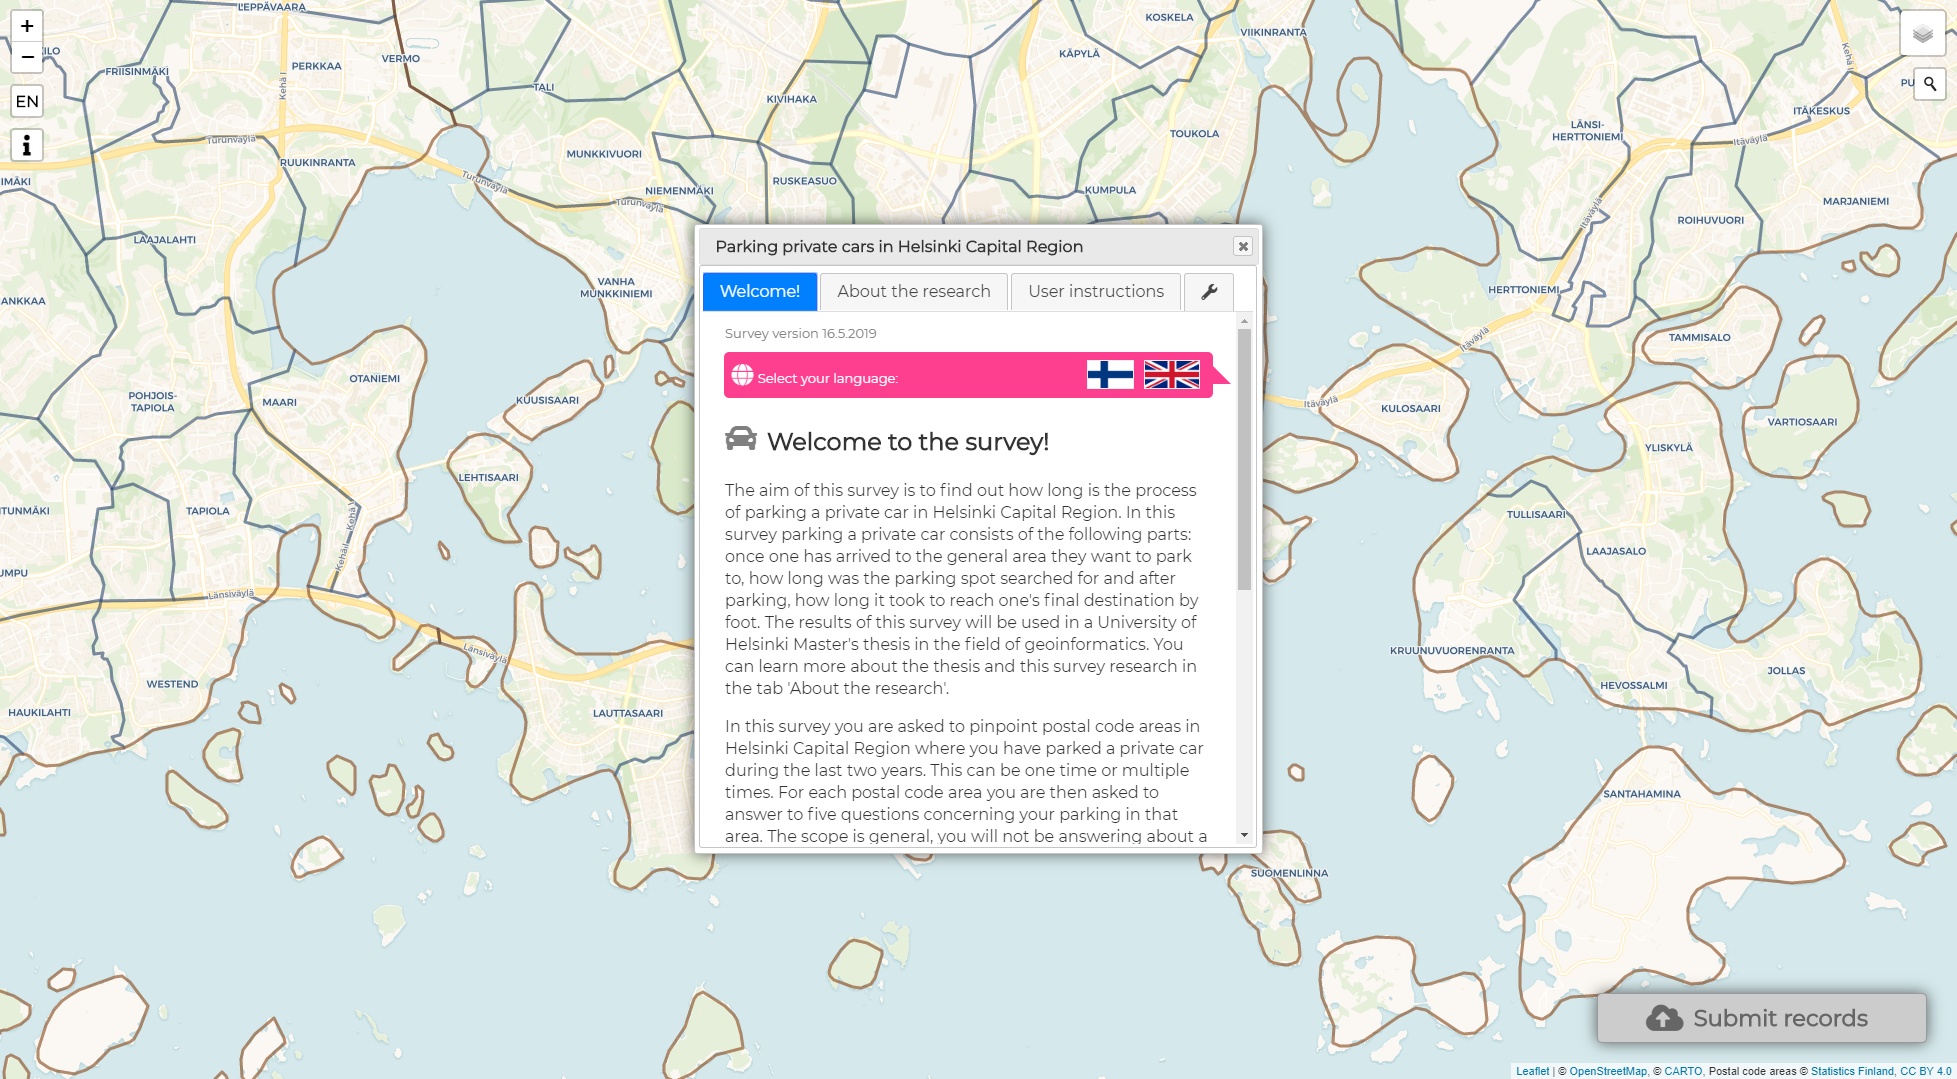
\includegraphics[width=\textwidth]{images/js_survey_welcome.png}
    \caption[Survey landing page]{The parking survey initial view with the welcoming dialog window.}%
    \label{fig:js_survey_welcome}%
\end{figure}

The survey front-end was programmed in NetBeans \gls{ide} 8.2 in mostly JavaScript using an open-source mapping library Leaflet (software version 1.4.0) in January--May 2019. In the survey, the respondent was presented with a map view of Helsinki Capital Region with its 167 postal code areas with the ability to drag the view, zoom in and out, search for places and addresses, choose the language between English and Finnish, and tweak various other settings to their liking. In this web survey, the respondent was asked to pick as many postal code areas as they could remember parking in in the last two years, and answer to five questions per each postal code area (table~\ref{tab:js_survey_questions} and figure~\ref{fig:js_survey_questions}). In each question, the respondent was asked to estimate their parking experience in that postal code area usually during the past two years. The last two years was chosen as the timeframe to allow respondents to comfortably recall parking events which happened during the subjective notion of "recent memory" while also forbidding the submission of out of date parking times. 

\textcolor{red}{lisää kappale, jossa selitän kysymysten sisällön auki, tsekkaa apu surveystä} The maximum values for searching for parking and walking to destination were consciously placed to 99 in an effort for the range to not feel restrictive for thes survey respondent.

In the introduction to the survey, it was explained to respondents that all answers were meant to be estimates as the survey was not about an exact time and place. To mitigate confusion and errors made by respondents a comprehensive help functionality and a location search tool were implemented in the parking survey. Once the respondent was finished with the survey, they would send their responses to the server. Respondents were welcomed to return to the survey to send additional data on any postal code areas they had missed the last time.

\begin{hyphenrules}{nohyphenation}
    \begin{table}[H]
        \centering
        \caption{Survey questions and question choices.} 
        \label{tab:js_survey_questions}
        \def\arraystretch{1.5}
        \setlength\tabcolsep{1.2ex}
        \begin{tabular}{ @{} >{\raggedright\arraybackslash}p{5.5cm} >{\raggedright\arraybackslash}p{5cm} >{\raggedright\arraybackslash}p{2.5cm} >{\raggedright\arraybackslash}p{2cm} @{} }
            \toprule
            Question & Question choices & Question type & Abbreviation \\
            \midrule
            How long does it usually take for you to find a parking spot and park your car in this postal code area (in minutes)? & 0--99 & Field, selection within range & parktime \\
            How long does it usually take for you to walk from your parking spot to your destination in this postal code area (in minutes)? & 0--99 & Field, selection within range & walktime \\
            How familiar are you with this postal code area? & 1 -- Extremely familiar\linebreak2 -- Moderately familiar\linebreak3 -- Somewhat familiar\linebreak4 -- Slightly familiar\linebreak5 -- Not at all familiar & Radio button group, likert-type scale & likert \\
            What kind of parking spot do you usually take in this postal code area? & 1 -- Parking space on the side of the street\linebreak2 -- Parking lot\linebreak3 -- Parking garage\linebreak4 -- Private or reserved spot\linebreak5 -- Other & Dropdown, selection & parkspot \\
            At what time of the day do you usually park in this postal code area? & 1 -- Weekday, rush hour (07.00--09.00 and 15.00--17.00)\linebreak2 -- Weekday, other than rush hour\linebreak3 -- Weekend\linebreak4 -- None of the above, no usual time & Dropdown, selection & timeofday \\
            \bottomrule
        \end{tabular}
    \end{table} 
\end{hyphenrules}

\begin{figure}[H]%
    \centering
    \subfloat[Survey questions in English.]{{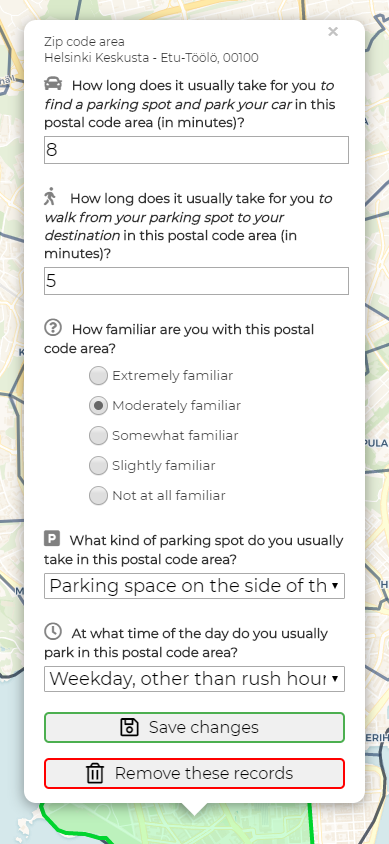
\includegraphics[width=6.25cm]{js_survey_en.png} }}%
    \qquad
    \subfloat[Survey questions in Finnish.]{{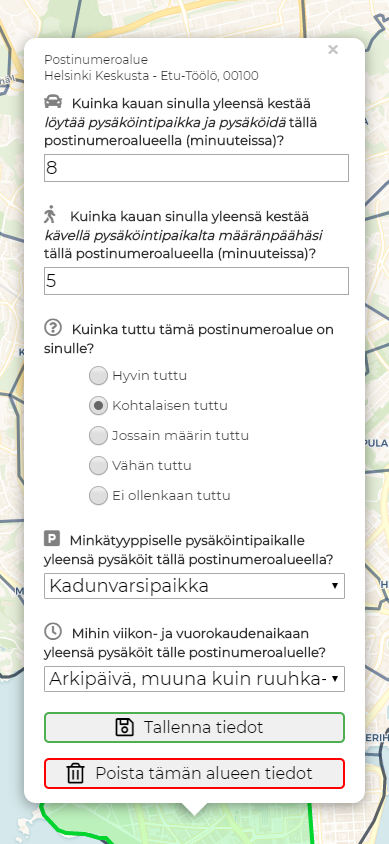
\includegraphics[width=6.25cm]{js_survey_fi.png} }}%
    \caption[Research survey questions in the web application]{For each postal code area of their choosing the respondent would answer to these five questions. The survey was made available in English and Finnish.}%
    \label{fig:js_survey_questions}%
\end{figure}

When data was received from the respondent, a script written in \gls{php} verified the data contents. This was an effort to prevent attacks on the web server running the study survey. Only specific variables of specific types were accepted from the front-end. Additionally, the \gls{php} verification made sure falsified or incomplete data would not be accepted into the database containing the verified results. If the server-side verification test failed in any way, the respondent was informed about it. 

In addition to the data verification, a PHP script tracked the IP addresses which accessed the survey web server. By using the survey, respondents agreed that their IP addresses were recorded for the use of this thesis solely to identify falsified or overlapping data and detect unique visits. All IP addresses were anonymised with a Python script and original sensitive data deleted. The anonymisation script is available for viewing at the thesis data analysis repository at GitHub (\textcolor{blue}{\url{https://github.com/sampoves/Msc-thesis-data-analysis}}).

As a final survey component, the server side contained two MySQL datatables, one for received data (table~\ref{tab:mysql_records}) and another for survey web page hits (table~\ref{tab:mysql_visitors}). In the table \textit{records}, the following data was recorded: time of sending (column name \code{timestamp}), IP address (\code{ip}), postal area code (\code{zipcode}), a value in the sequence 1--5 for the likert question (\code{likert}), a value in the sequence 1--5 for the question what type of parking spot was used (\code{parkspot}), an integer value for how long it usually took to park in this location (\code{parktime}), an integer value for how long it usually took to walk from parking place to one's destination (\code{walktime}), and a value in the sequence 1--4 for the question at what time of the day one usually parks in the location (\code{timeofday}) (table~\ref{tab:mysql_records_str}). In the table \textit{records}, it is notable that in the case an respondent sent the web server data for multiple postal code areas each of the postal code areas would take up their own row in the data table. Consequently, it was theoretically possible for one respondent to simultaneously submit 167 rows of data.

In the table \textit{visitors}, the following data was recorded: IP address (\code{ip}), the timestamp of the first visit of this IP address (\code{ts\_first}), the timestamp of latest visit of this IP address (\code{ts\_latest}), and the count of visits (\code{count}). In this table, an IP address is only stored once. On the first visit of an IP address, the row for that IP address is created in the data table with \code{ts\_first} and \code{ts\_latest} being identical. On further visits of that IP address the original row is appended with updated information in the columns \code{ts\_latest} and \code{count} (table~\ref{tab:mysql_visitors_str}).

\begin{hyphenrules}{nohyphenation}
    \begin{table}[H]
        \centering
        \setlength\tabcolsep{1.2ex}
        \caption[Structure of MySQL table records]{The structure of the survey MySQL table \textit{records} fetched with the statement \code{DESCRIBE records;}} 
        \label{tab:mysql_records_str}
        \begin{tabular}{ @{} >{\raggedright\arraybackslash}p{2cm} >{\raggedright\arraybackslash}p{2cm} >{\raggedright\arraybackslash}p{1cm} >{\raggedright\arraybackslash}p{1cm} >{\raggedright\arraybackslash}p{1.5cm} >{\raggedleft\arraybackslash}p{4cm} @{} }
            \toprule
            Field & Type & Null & Key & Default & Extra \\
            \midrule
            id & int(11) & No & PRI & NULL & AUTO\_INCREMENT \\
            timestamp & varchar(19) & Yes & & NULL & \\
            ip & TEXT & Yes & & NULL & \\
            zipcode & varchar(5) & Yes & & NULL & \\
            likert & int(1) & Yes & & NULL & \\
            parkspot & int(1) & Yes & & NULL & \\
            parktime & int(2) & Yes & & NULL & \\
            walktime & int(2) & Yes & & NULL & \\
            timeofday & int(1) & Yes & & NULL & \\
            \bottomrule
        \end{tabular}
    \end{table} 
\end{hyphenrules}

\begin{hyphenrules}{nohyphenation}
    \begin{table}[H]
        \centering
        \setlength\tabcolsep{1.2ex}
        \caption[Structure of MySQL table visitors]{The structure of the survey MySQL table \textit{visitors} fetched with the statement \code{DESCRIBE visitors;}} 
        \label{tab:mysql_visitors_str}
        \begin{tabular}{ @{} >{\raggedright\arraybackslash}p{2cm} >{\raggedright\arraybackslash}p{2cm} >{\raggedright\arraybackslash}p{1cm} >{\raggedright\arraybackslash}p{1cm} >{\raggedright\arraybackslash}p{1.5cm} >{\raggedleft\arraybackslash}p{4cm} @{} }
            \toprule
            Field & Type & Null & Key & Default & Extra \\
            \midrule
            id & int(11) & No & PRI & NULL & AUTO\_INCREMENT \\
            ip & TEXT & Yes & & NULL & \\
            ts\_first & DATETIME & Yes & & NULL & \\
            ts\_latest & DATETIME & Yes & & NULL & \\
            count & int(11) & Yes & & NULL & \\        
            \bottomrule
        \end{tabular}
    \end{table} 
\end{hyphenrules}

The parking survey was released to the public in May 2019 and the active phase of collecting data continued until 30th June 2019. However, the survey remained open after thiss active period, receiving the last row of data in October 2019. The majority of the respondents were found through Facebook. Invitations to participate in the survey were sent to 112 city district and neighborhood groups with a theoretical reach of tens of thousands of people. Of the 112 posts, 63 were Helsinki centric groups, while 22 were from Espoo, 15 from Vantaa, and 12 from municipalities bordering Helsinki Capital Region. In addition to these city district and municipal groups, invitation to participate was sent to two other Facebook groups, "Lisää kaupunkia Helsinkiin", a group for city planning ethusiasts in Helsinki, and the GIS profession group "GIS-velhot". It is not possible to conclusively differentiate from which group or city survey data originated from. A clue about the survey's popularity in each city, however, may be gained from the table \textit{visitors} due to the fact that invitation posts were sent over multiple days to the groups in the order: 

\begin{displayquote}
$\text{Espoo}\rightarrow\text{Helsinki}\rightarrow\text{Vantaa}\rightarrow\text{bordering municipalities}\rightarrow\text{reminders to the largest groups}$
\end{displayquote}

In addition to Facebook, an effort was also made to get faculty members of geosciences and geography and students of University of Helsinki to participate in the survey. A small amount of answers were collected with a tweet sent from the Twitter account of Digital Geography Lab. After the initial invitation to participate, reminders were sent to the largest Facebook groups one month after the original posts.

The source code for the survey described in this chapter and step-by-step information to set up an identical system is available at GitHub (\textcolor{blue}{\url{https://github.com/sampoves/parking-in-helsinki-region}}). As a side product, a variant of this survey was created where respondents pick precise points instead of areas. This point-based survey template is, too, available at GitHub (\textcolor{blue}{\url{https://github.com/sampoves/leaflet-map-survey-point}}). The parking survey web application as it was used in this thesis may be tested in the following web address: \textcolor{blue}{\url{https://parking-survey.socialsawblade.fi}}.

% \scalebox to prevent table going too wide
\begin{hyphenrules}{nohyphenation}
    \begin{table}[H]
        \centering
        \setlength\tabcolsep{2pt}
        \caption[MySQL table records]{An excerpt of the data content of the research survey MySQL table \textit{records}.} 
        \label{tab:mysql_records}
        \scalebox{0.9}
        {\begin{tabular}{ @{} >{\raggedright\arraybackslash}p{1.5cm} >{\raggedright\arraybackslash}p{4cm} >{\raggedright\arraybackslash}p{2.5cm} >{\raggedright\arraybackslash}p{2cm} >{\raggedright\arraybackslash}p{1.5cm} >{\raggedright\arraybackslash}p{1.5cm} >{\raggedright\arraybackslash}p{1.5cm} >{\raggedright\arraybackslash}p{1.5cm} >{\raggedright\arraybackslash}p{1.5cm} @{} }
            \toprule
            id & timestamp & ip & zipcode & likert & parkspot & parktime & walktime & timeofday \\
            \midrule
            3245 & 2019-06-06 21:41:21 & wro4qo8hv4 & 00510 & 1 & 4 & 0 & 3 & 1 \\
            3246 & 2019-06-06 21:41:54 & aonm72lyx3 & 00520 & 2 & 1 & 10 & 5 & 1 \\
            3247 & 2019-06-06 21:46:19 & n1982i4i2v & 00100 & 1 & 1 & 20 & 4 & 1 \\
            3248 & 2019-06-06 21:46:22 & sbhfz0uvsl & 00210 & 1 & 1 & 5 & 3 & 3 \\
            3249 & 2019-06-06 21:46:22 & sbhfz0uvsl & 00220 & 2 & 2 & 5 & 5 & 2 \\        
            \bottomrule
        \end{tabular}}
    \end{table} 
\end{hyphenrules}

\begin{hyphenrules}{nohyphenation}
    \begin{table}[H]
        \centering
        \setlength\tabcolsep{1pt}
        \caption[MySQL table visitors]{An excerpt of the data content of the research survey MySQL table \textit{visitors}.} 
        \label{tab:mysql_visitors}
        \begin{tabular}{ @{} >{\raggedright\arraybackslash}p{2cm} >{\raggedright\arraybackslash}p{3cm} >{\raggedright\arraybackslash}p{4cm} >{\raggedright\arraybackslash}p{4cm} >{\raggedleft\arraybackslash}p{1cm} @{} }
            \toprule
            id & ip & ts\_first & ts\_latest & count \\
            \midrule
            1780 & mvovd467a7 & 2019-05-26 15:25:23 & 2019-05-26 15:26:06 & 2 \\
            1781 & xgbgkkzxb3 & 2019-05-26 15:26:23 & 2019-05-26 15:26:23 & 1 \\
            1782 & c9qer4q99a & 2019-05-26 15:27:25 & 2019-05-26 15:27:25 & 1 \\
            1783 & cujhd0hng7 & 2019-05-26 15:27:29 & 2019-05-26 15:27:29 & 1 \\
            1784 & 3ja7gjtko6 & 2019-05-26 15:28:45 & 2019-05-26 15:29:20 & 2 \\        
            \bottomrule
        \end{tabular}
    \end{table} 
\end{hyphenrules}

\begin{figure}[H]%
    \centering
    \subfloat[Respondent arrives to the survey web application to see a map with the postal code areas of Helsinki Capital Region lined out.]{{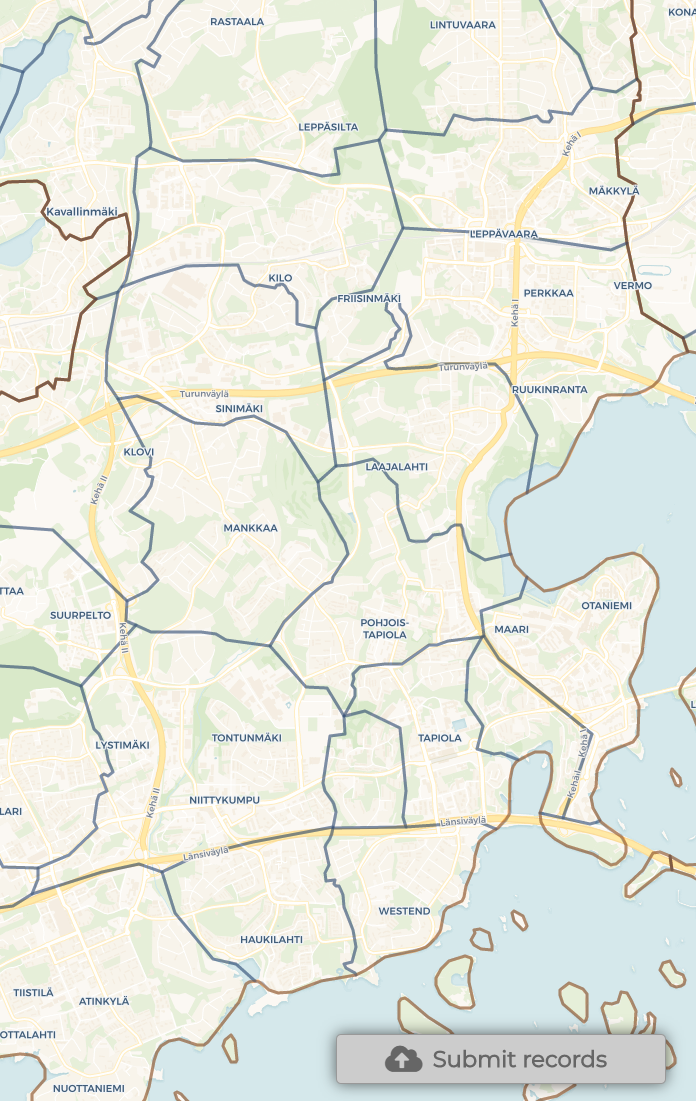
\includegraphics[width=7cm]{js_survey_process1.png} }}%
    \quad
    \subfloat[Respodent proceeds to fill out their parking experiences in freely chosen postal code areas.]{{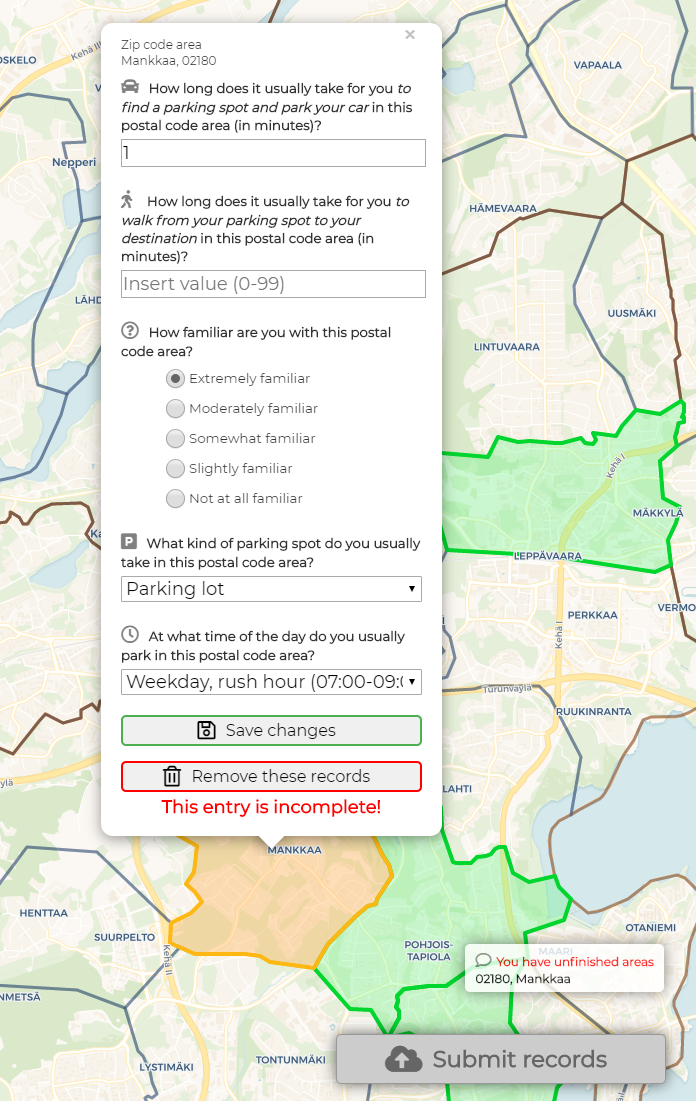
\includegraphics[width=7cm]{js_survey_process2.png} }}%
    \quad
    \subfloat[\textit{Submit records} button activates when all questions in all selected postal code areas are completed.]{{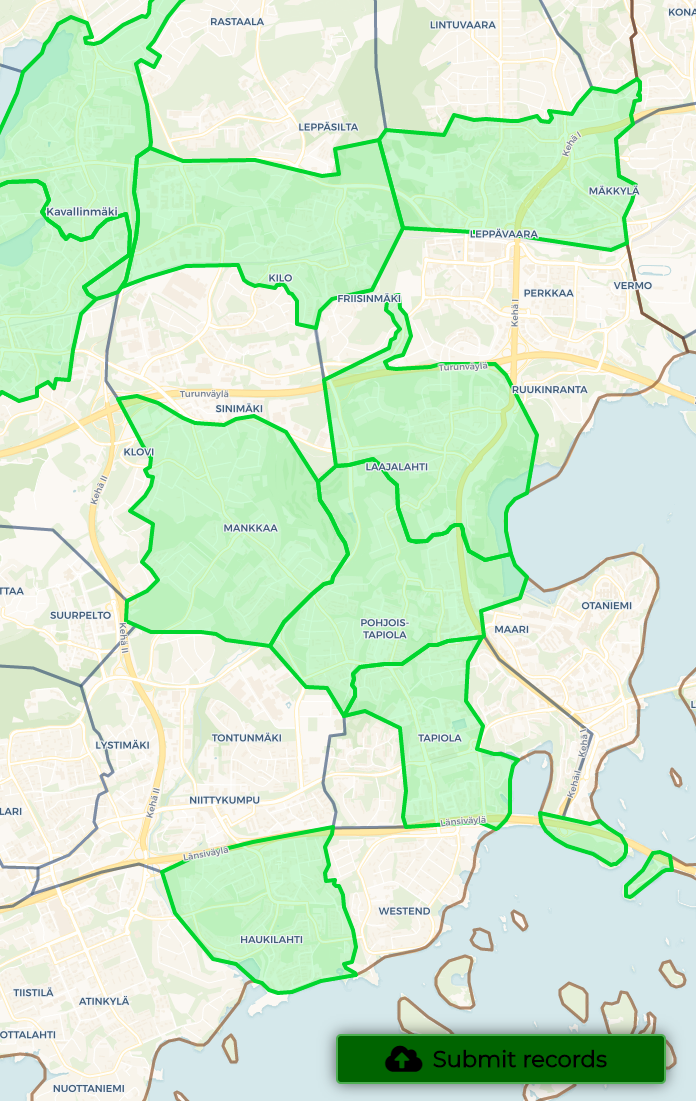
\includegraphics[width=7cm]{js_survey_process3.png} }}%
    \quad
    \subfloat[Respondent receives a prompt to confirm that their submission was successful.]{{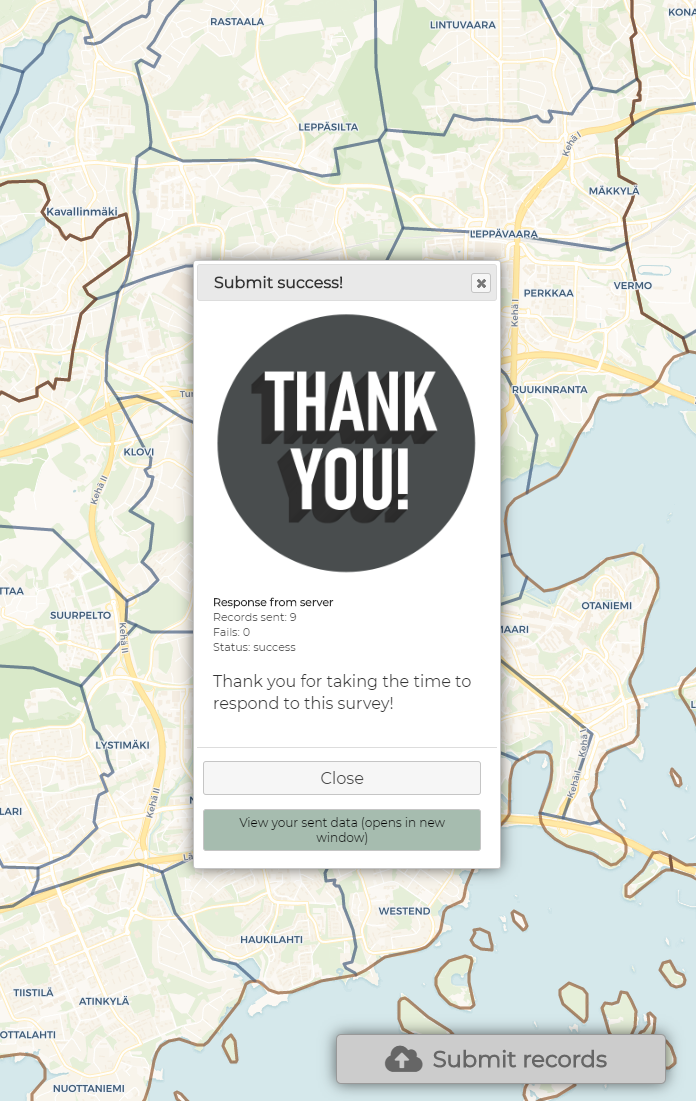
\includegraphics[width=7cm]{js_survey_process4.png} }}%
    \caption[Steps to fill out the survey]{A respondent would follow these steps to submit data through the survey web application.}%
    \label{fig:survey_process}%
\end{figure}

\newpage
\subsection{Processing survey data}
\label{sec:processdata} % labeling to enable hyperref to this chapter
\justify
%\begin{itemize} %processingin tärkeimmät kohdat
%    \item anonymisation of ip addresses
%    \item Read in spatial data sources
%    \item Read in survey data
%    \item Prepare source data (convert formats, remove some irregular erroneous answers from dataset)
%    \item Prepare shape files (remove islands not reachable by car)
%    \item give grid cells zipcodes (ykr grid does not have those of-the-shelf. Develop method to assign all cells zipcodes, take into account water and grid cells which are outside of research area)
%    \item respondent behaviour (see how each user has answered)
%    \item detect illegal data (first detect duplicate answers, produce report. Then remove data where parktime and/or walktime is 60 or over)
%    \item Add data to geodataframes (add columns for ykr\_vyoh, ua-forest, answer count, parktime and walktime mean
%    \item show statistics to user
%    \item Set percentage of urban zones and forest in each zipcode area (choose one urban zone and forest amount (jenks breaks) for every zipcode)
%    \item add subdivisions to data (all answer row gets corresponding subdivision value)
%    \item EXPERIMENTAL utilise travel-time matrix 2018, make comparisons
%    \item EXPERIMENTAL somehow create my own TTM18, with updated values
%    \item export results to R
%\end{itemize}

In this section, various data are refered to with abbreviated names as this makes it easier to follow the data processing workflow. Please see table~\ref{tab:used_data} for the key. \textcolor{red}{kaikki kohdat tässä kappaleessa ei käytä lyhenteitä (records, visitors, postal)}

The main objective of the thesis data processing was to merge survey responses (\textit{records}) with selected spatial data and prepare \textit{records}, survey visits (\textit{visitors}), \textit{postal}, and \textit{grid} for later analysis in R programming language environment. Using a selection of open spatial data (table~\ref{tab:used_data}), new explanatory variables would be available for use in the analysis. This opened opportunities to compare the newly gathered survey data against that in Helsinki Travel-time Matrix 2018. \textcolor{red}{toistoa} \textcolor{purple}{All data processing in this phase was carried out in Python programming language version 3.7.6, using Anaconda, a free and open-source Python distribution for scientific programming. Anaconda version 2020.02 included all essential packages for carrying out the script, with the exception of GeoPandas 0.5.0, the package for geospatial data manipulation in Python. GeoPandas and its dependencies -- GDAL 2.4.1, Fiona 1.8.6, pyproj 2.1.3, rtree 0.8.3, and Shapely 1.6.4.post1 -- were manually installed through Python package installer pip (table~\ref{tab:used_soft})}.

As the first step in the survey data processing, all IP addresses were anonymised and replaced with identifiers of ten characters consisting of numbers 0--9 and letters of English alphabet (figure~\ref{fig:gen_workflow}, section 1). The anonymisation was carried out in such a way that the random identifiers for respondents matched in both \textit{records} and \textit{visitors}, preserving the possibility to associate survey responses with survey visits. 

\begin{figure}[H]%
    \centering
    \subfloat[Unedited PAAVO postal code areas for Helsinki Capital Region.]{{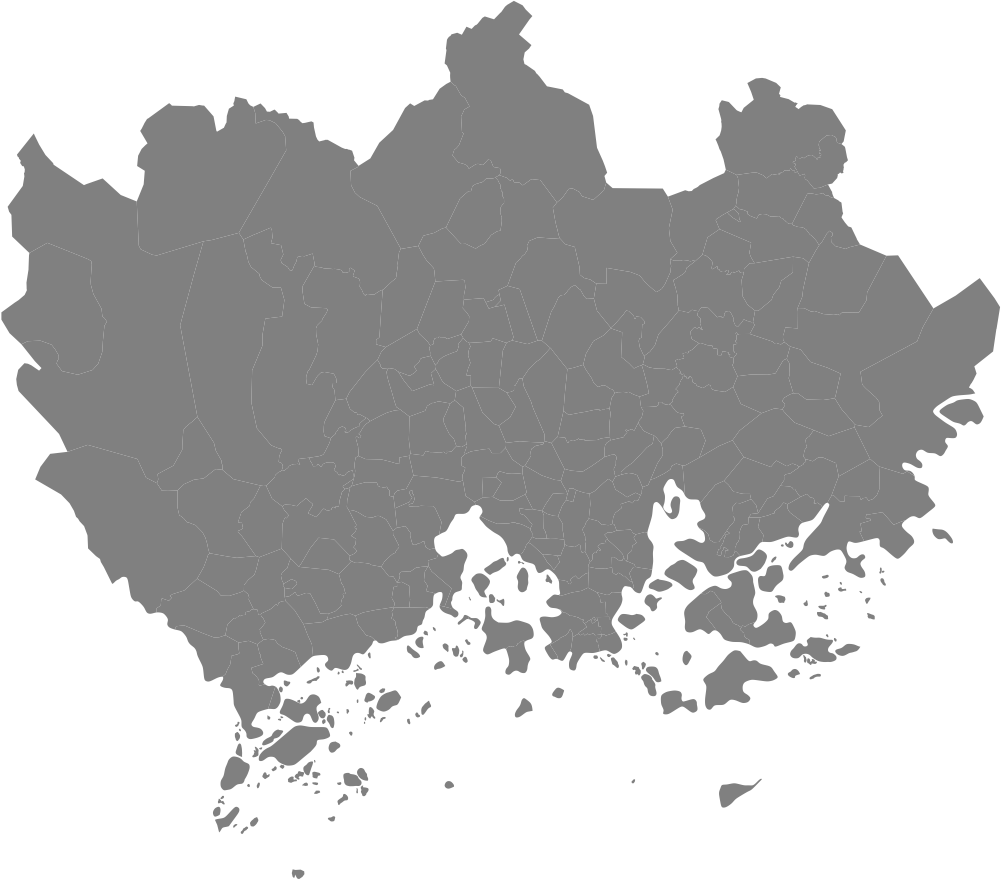
\includegraphics[width=8.1cm]{resarea_unedited.png} }}%
    \quad
    \subfloat[PAAVO postal code areas for Helsinki Capital Region, islands unreachable by car removed.]{{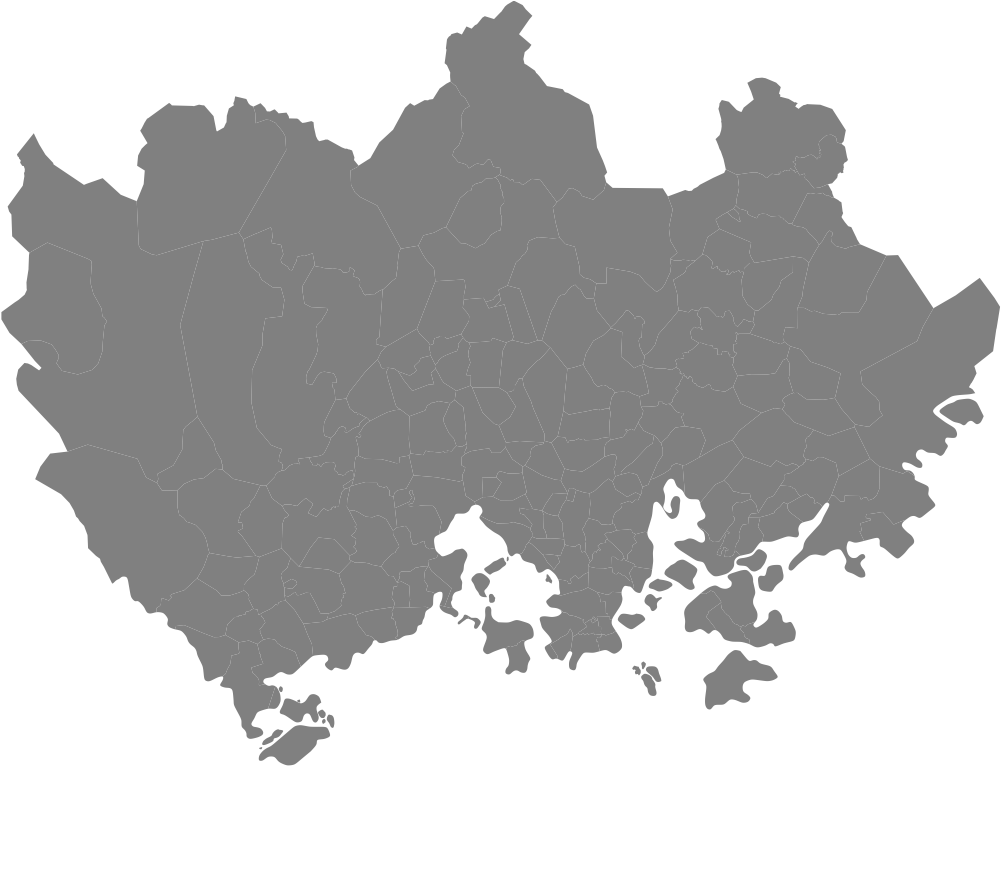
\includegraphics[width=8.1cm]{resarea_edited.png} }}%
    \caption[Process to remove islands not reachable by car]{Islands unreachable by car were removed from the postal code area data in the Python data processing.}%
    \label{fig:paavo_resarea}%
\end{figure}

The data processing proper started with loading the open spatial data presented in table~\ref{tab:used_data} and selecting only areas relevant to the research (figure~\ref{fig:gen_workflow}, section 2). For \textit{CORINE}, this meant selecting only areas marked Level1Eng, Artificial surfaces. \textit{YKR zones}, a dataset that covers the entirety of Finland, was clipped with spatial dimensions of PAAVO postal code areas data, \textit{postal}, that had been extended with a 500 meter buffer. \textit{postal} was processed to only include areas reachable by car from the mainland (figure~\ref{fig:paavo_resarea}). Islands not reachable by car were approximated visually using Google Maps and were removed from the data. However, some islands in Helsinki Capital Region are technically accessible with a car from the mainland, but in practice the access is limited. In these cases, deliberation was used. For example, Suomenlinna islands and Korkeasaari were kept in the data. Conversely, some technically car-accessible islands like Staffan in Espoo, and Mustasaari and Seurasaari in Helsinki were removed from the data with the grounds of them containing only private property, or no public parking spaces. \textcolor{red}{selitä laajemmin miksi näitä saaria poistellaan (analyysi ja visualisointi). lisäksi, mieti toi logiikka "yksityisalue tai ei yleisiä parkkiksia"}

\begin{figure}[H]%
    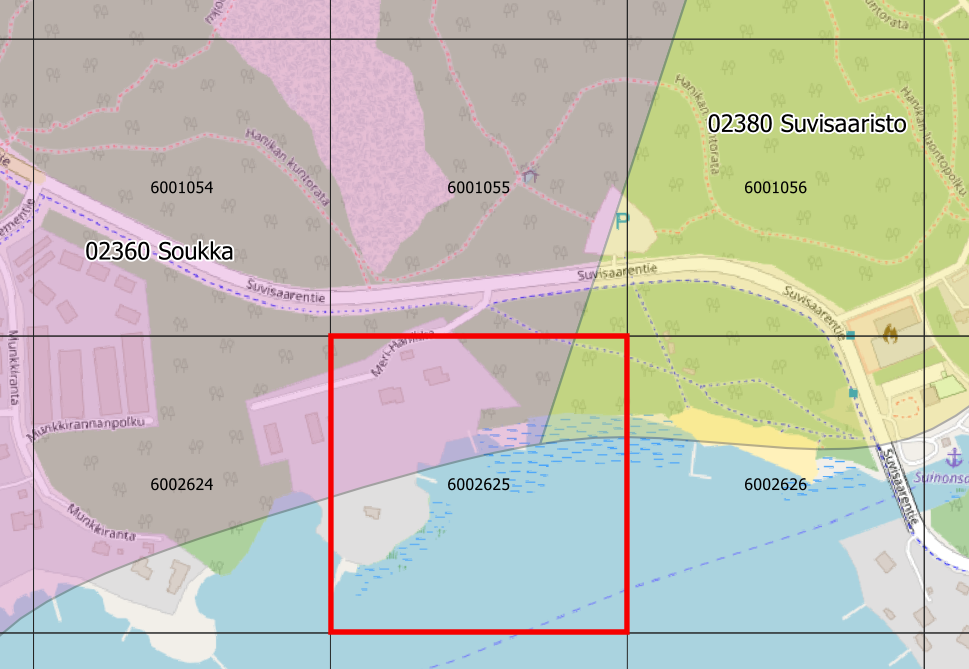
\includegraphics[width=\textwidth]{images/paavo-ykr.png}
    \caption[Assigning MetropAccess-YKR-grid postal codes]{The MetropAccess-YKR-grid cell 6002625 (marked with the red square) is assigned postal code 02360 because in that grid cell, the largest segment of PAAVO open data (coloured warm purple and yellow) belongs in the postal code 02360 Soukka. \textcolor{red}{osm cite}}%
    \label{fig:paavo_ykr}%
\end{figure}

Helsinki Region Travel Time Matrix 2018 and the survey data of this thesis operate in different spatial units. Travel time Matrix 2018 uses the MetropAccess-YKR-grid (\textit{grid}), a spatial dataset based on the Statistics Finland statistical grid with the cell size of 250 x 250 meters. The basic spatial unit of the survey data is the postal code area based on PAAVO open data (\textcolor{red}{lisää lähteet}). Using Python, postal codes were added to each \textit{grid} cell with the logic that the largest area in \textit{postal} (figure~\ref{fig:paavo_ykr}) assigns the postal code in each \textit{grid} cell. \textit{postal} polygons do not always intersect with the cells of \textit{grid} and because of this some cells were assigned a postal code of 99999 to denote missing data (\textcolor{red}{mieti vielä 99999:n käyttö}). As a side product of this postal code assignment, \textit{grid} was merged with data which tells how much of a cell was contained in the research area (\textit{postal}) and how large was the largest postal code area which dictated the postal code assignment of the current cell. \textcolor{red}{varmista että lukija ymmärtää PAAVO spatial datan ja tutkimusalueen yhteyden}

The data processing script created for this thesis contains detailed features to detect patterns in the survey data (figure~\ref{fig:gen_workflow}, section 3). To enhance pattern recognition, \textit{records} and \textit{visitors} were purged of known false data, which were namely responses and visits made by me.

The data processing script creates two distinct reports about \textit{records}. Firstly, the data processing script aggregates \textit{records} by IP address code, resulting in an Excel file where one row represents each respondent. It is then possible to review the behaviour of each respondent in detail. In addition to this report, the data processing script writes a text file report about IP address codes which submitted multiple responses from the same postal code area. The text file report also identifies whether the duplicate responses for each postal code area per each IP address code have identical values or if they have changed between responses. These two reports were used to determine what to do about the duplicates and values which appear anomalous.

It was decided that if the parking time or walking time value in a \textit{records} row was 60 minutes or greater, that data row would be deleted. This value is arbitrary. The research assumes that it is highly unlikely that anybody would generally park 60 minutes away from their final destination to which they would then proceed on foot. A hour of searching for parking is plausible in the center of Helsinki but because of its unlikeliness the same 60 minutes limit was utilised in searching for parking. It is not possible to determine why multiple survey responses contain the maximum value for parktime and walktime, 99, but it can not be ruled out that these data rows are protest votes meant to declare that reliable parking is hard to find in certain parts of Helsinki Capital Region. When advertising the thesis survey on Facebook, some people took the opportunity to voice their displeasure at the perceivedly difficult parking conditions in the Helsinki Capital Region. In conclusion, even though the Python script has the capability to delete data rows deemed illegal, all of the illegal data in \textit{records} was preserved a more versatile analysis in R.

Next in the survey data processing workflow the additional spatial data was added to \textit{postal}, the dataset with one row for each postal code area (figure~\ref{fig:gen_workflow}, section 4). Utilising \textit{records}, functions \code{sum}, \code{mean}, and \code{median} were used to produce answer count, and means and medians for parktime and walktime for all postal code areas. Each postal code area also received seven columns to depict the share of \textit{YKR zones} classes in percentage. It must be noted that before applying the \textit{YKR zones} data to the thesis data, classification in the source data was simplified with following the notation presented by the research group at the websites of the zones of urban structure (table~\ref{tab:ykr_zones_simplify}, \cite{FinnishEnvironmentInstitute2013}). Using \textit{CORINE} data, the percentage of artificial surface in each postal code area was calculated (table~\ref{tab:corine_artificial}).

\begin{hyphenrules}{nohyphenation}
    \begin{table}[H]
        \centering
        \def\arraystretch{1.2}
        \setlength\tabcolsep{1.2ex}
        \caption[YKR zones processing]{The logic by which the unedited source data for zones of urban structure was transformed for this thesis.}
        \label{tab:ykr_zones_simplify}
        \scalebox{0.9}
        {\begin{tabular}{ @{} >{\raggedright\arraybackslash}p{6cm} >{\raggedright\arraybackslash}p{6cm} @{} }
            \toprule
            Original definition & Definition for this thesis \\
            \midrule
            Keskustan jalankulkuvyöhyke & Keskustan jalankulkuvyöhyke \\
            \greyrule
            % Manually set the position of multirow label
            Keskustan reunavyöhyke & \multirow{3}{*}[-4.5ex]{Keskustan reunavyöhyke} \\
            Keskustan reunavyöhyke/intensiivinen joukkoliikenne & \\
            Keskustan reunavyöhyke/joukkoliikenne & \\
            \greyrule
            Alakeskuksen jalankulkuvyöhyke & \multirow{3}{*}[-4.5ex]{Alakeskuksen jalankulkuvyöhyke} \\
            Alakeskuksen jalankulkuvyöhyke/intensiivinen joukkoliikenne & \\
            Alakeskuksen jalankulkuvyöhyke/joukkoliikenne & \\
            \greyrule
            Intensiivinen joukkoliikennevyöhyke & Intensiivinen joukkoliikennevyöhyke \\ 
            \greyrule
            Joukkoliikennevyöhyke & Joukkoliikennevyöhyke \\
            \greyrule
            Autovyöhyke & Autovyöhyke \\
            \greyrule
            \textit{Areas not in the YKR zones data} & novalue \\
            \bottomrule
        \end{tabular}}
    \end{table} 
\end{hyphenrules}

\begin{hyphenrules}{nohyphenation}
    \begin{table}[H]
        \centering
        \def\arraystretch{1.2}
        \setlength\tabcolsep{1.2ex}
        \caption[CORINE data levels]{CORINE land cover 2018 data hierarchy under attribute data column Level1Eng, Artificial surfaces.}
        \label{tab:corine_artificial}
        \scalebox{0.85}
        {\begin{tabular}{ @{} >{\raggedright\arraybackslash}p{4cm} @{} >{\raggedright\arraybackslash}p{4cm} @{} >{\raggedright\arraybackslash}p{4.25cm} @{} >{\raggedright\arraybackslash}p{4cm} @{} }
            \toprule
            Level1, Level1Eng & Level2, Level2Eng & Level3, Level3Eng & Level4, Level4Eng \\
            \midrule
            \multirow{16}{4cm}[-15ex]{1 Artificial surfaces} & \multirow{2}{4cm}[-4ex]{11 Urban fabric} & 111 Continuous urban fabric 
 & 1111 Continuous urban fabric \\
            \arrayrulecolor{black!30}\cmidrule(lr){3-4}
            & & 112 Discontinuous urban fabric & 1121 Discontinuous urban fabric \\
            \arrayrulecolor{black!30}\cmidrule(lr){2-4}
            & \multirow{2}{4cm}[-0.5ex]{12 Urban fabric} & \multirow{2}{4cm}{121 Industrial or commercial units} & 1211 Commercial units \\
            \arrayrulecolor{black!30}\cmidrule(lr){4-4}
            & & & 1212 Industrial units \\
            \arrayrulecolor{black!30}\cmidrule(lr){2-4}
            & \multirow{3}{4cm}[-4ex]{12 Industrial, commercial and transport units} & 122 Road and rail networks and associated land & 1221 Road and rail networks and associated land \\
            \arrayrulecolor{black!30}\cmidrule(lr){3-4}
            & & 123 Port areas & 1231 Port areas \\
            \arrayrulecolor{black!30}\cmidrule(lr){3-4}
            & & 124 Airports & 1241 Airports \\
            \arrayrulecolor{black!30}\cmidrule(lr){2-4}
            & \multirow{4}{4cm}[-4ex]{13 Mine, dump and construction sites} & \multirow{2}{4cm}[-2.5ex]{131 Mineral extraction sites} & 1311 Mineral extraction sites \\
            \arrayrulecolor{black!30}\cmidrule(lr){4-4}
            & & & 1312 Open cast mines \\
            \arrayrulecolor{black!30}\cmidrule(lr){3-4}
            & & 132 Dump sites & 1321 Dump sites \\
            \arrayrulecolor{black!30}\cmidrule(lr){3-4}
            & & 133 Construction sites & 1331 Construction sites \\
            \arrayrulecolor{black!30}\cmidrule(lr){2-4}
            & \multirow{5}{4cm}[-2ex]{14 Artificial, non-agricultural vegetated areas} & 141 Green urban areas & 1411 Green urban areas \\
            \arrayrulecolor{black!30}\cmidrule(lr){3-4}
            & & \multirow{4}{4cm}[-3ex]{142 Sport and leisure facilities} & 1421 Summer cottages \\
            \arrayrulecolor{black!30}\cmidrule(lr){4-4}
            & & & 1422 Sport and leisure areas \\
            \arrayrulecolor{black!30}\cmidrule(lr){4-4}
            & & & 1423 Golf courses \\
            \arrayrulecolor{black!30}\cmidrule(lr){4-4}
            & & & 1424 Race courses \\
            \bottomrule
        \end{tabular}}
    \end{table} 
\end{hyphenrules}

% https://www.spatialanalysisonline.com/HTML/index.html?classification_and_clustering.htm
In the finalising section, \textit{records} was prepared for analysis and visualisation in R (figure~\ref{fig:gen_workflow}, section 5). The software library for plotting in R, \textit{ggplot2}, prefers data inputted in long format. To study charasteristics of postal code areas in this research, it meant adding repetitive data columns in \textit{records}, where values for CORINE land cover 2018 artificial surfaces, YKR zone and subdivision remained unchanged for all rows in the same postal code area. For artificial surfaces, a custom Jenks natural breaks function (GitHub user Drewda, \textcolor{red}{add cite, add jenks cite, kato kommenttilinkki}) with five classes were utilised to find the applicable Jenks breaks class for each postal code area. For YKR zones, the most common urban structure type in percentage was selected for each postal code area. In addition, \textit{records} was inserted with municipality subdivision information (figure~\ref{fig:subdiv_placement}). This was achieved by collecting data from the web sites of the municipalities of Helsinki Capital Region (\cite{Espoonkaupunki2020}, \cite{Helsinginkaupunkiymparistontoimiala2019}, \cite{Vantaankaupunki2019}). In these sources, each municipality broke the subdivisions down to city district level, from where it was possible to allot each postal code area with a subdivision. This was for the most part simplistic work, but in some cases the postal code areas and city districts did not align and author's own deliberation was used to help the placement. Some of the most glaring discrepancies between PAAVO postal code areas and subdivision boundaries occur in Espoo. In the case of Lippajärvi-Järvenperä, a postal code area north of Kauniainen, the subdivision Vanha-Espoo was chosen because Lippajärvi-Järvenperä as a whole does not fit into the charasteristics of Suur-Leppävaara, and at the same time the city districts Lippajärvi and Järvenperä do not fit into the distinctive features of the subdivision Pohjois-Espoo. In the same spirit the postal code area Sepänkylä-Kuurinniitty south of Kauniainen lies troublingly in the area of four subdivisions of Espoo. In the end Vanha-Espoo was chosen as Sepänkylä-Kuurinniitty lies for the most part in its area. Similar complications occurred in Helsinki and Vantaa (the partial placement of Kirkonkylä-Veromäki and Ruskeasanta-Ilola in subdivision of Tikkurila) and using my best judgement, the classification shown in figure~\ref{fig:subdiv_placement} was used in the survey results analysis of this thesis.

The source code for the data processing described in this chapter is available at GitHub (\textcolor{blue}{\url{https://github.com/sampoves/Msc-thesis-data-analysis}}).

\begin{figure}[H]%
    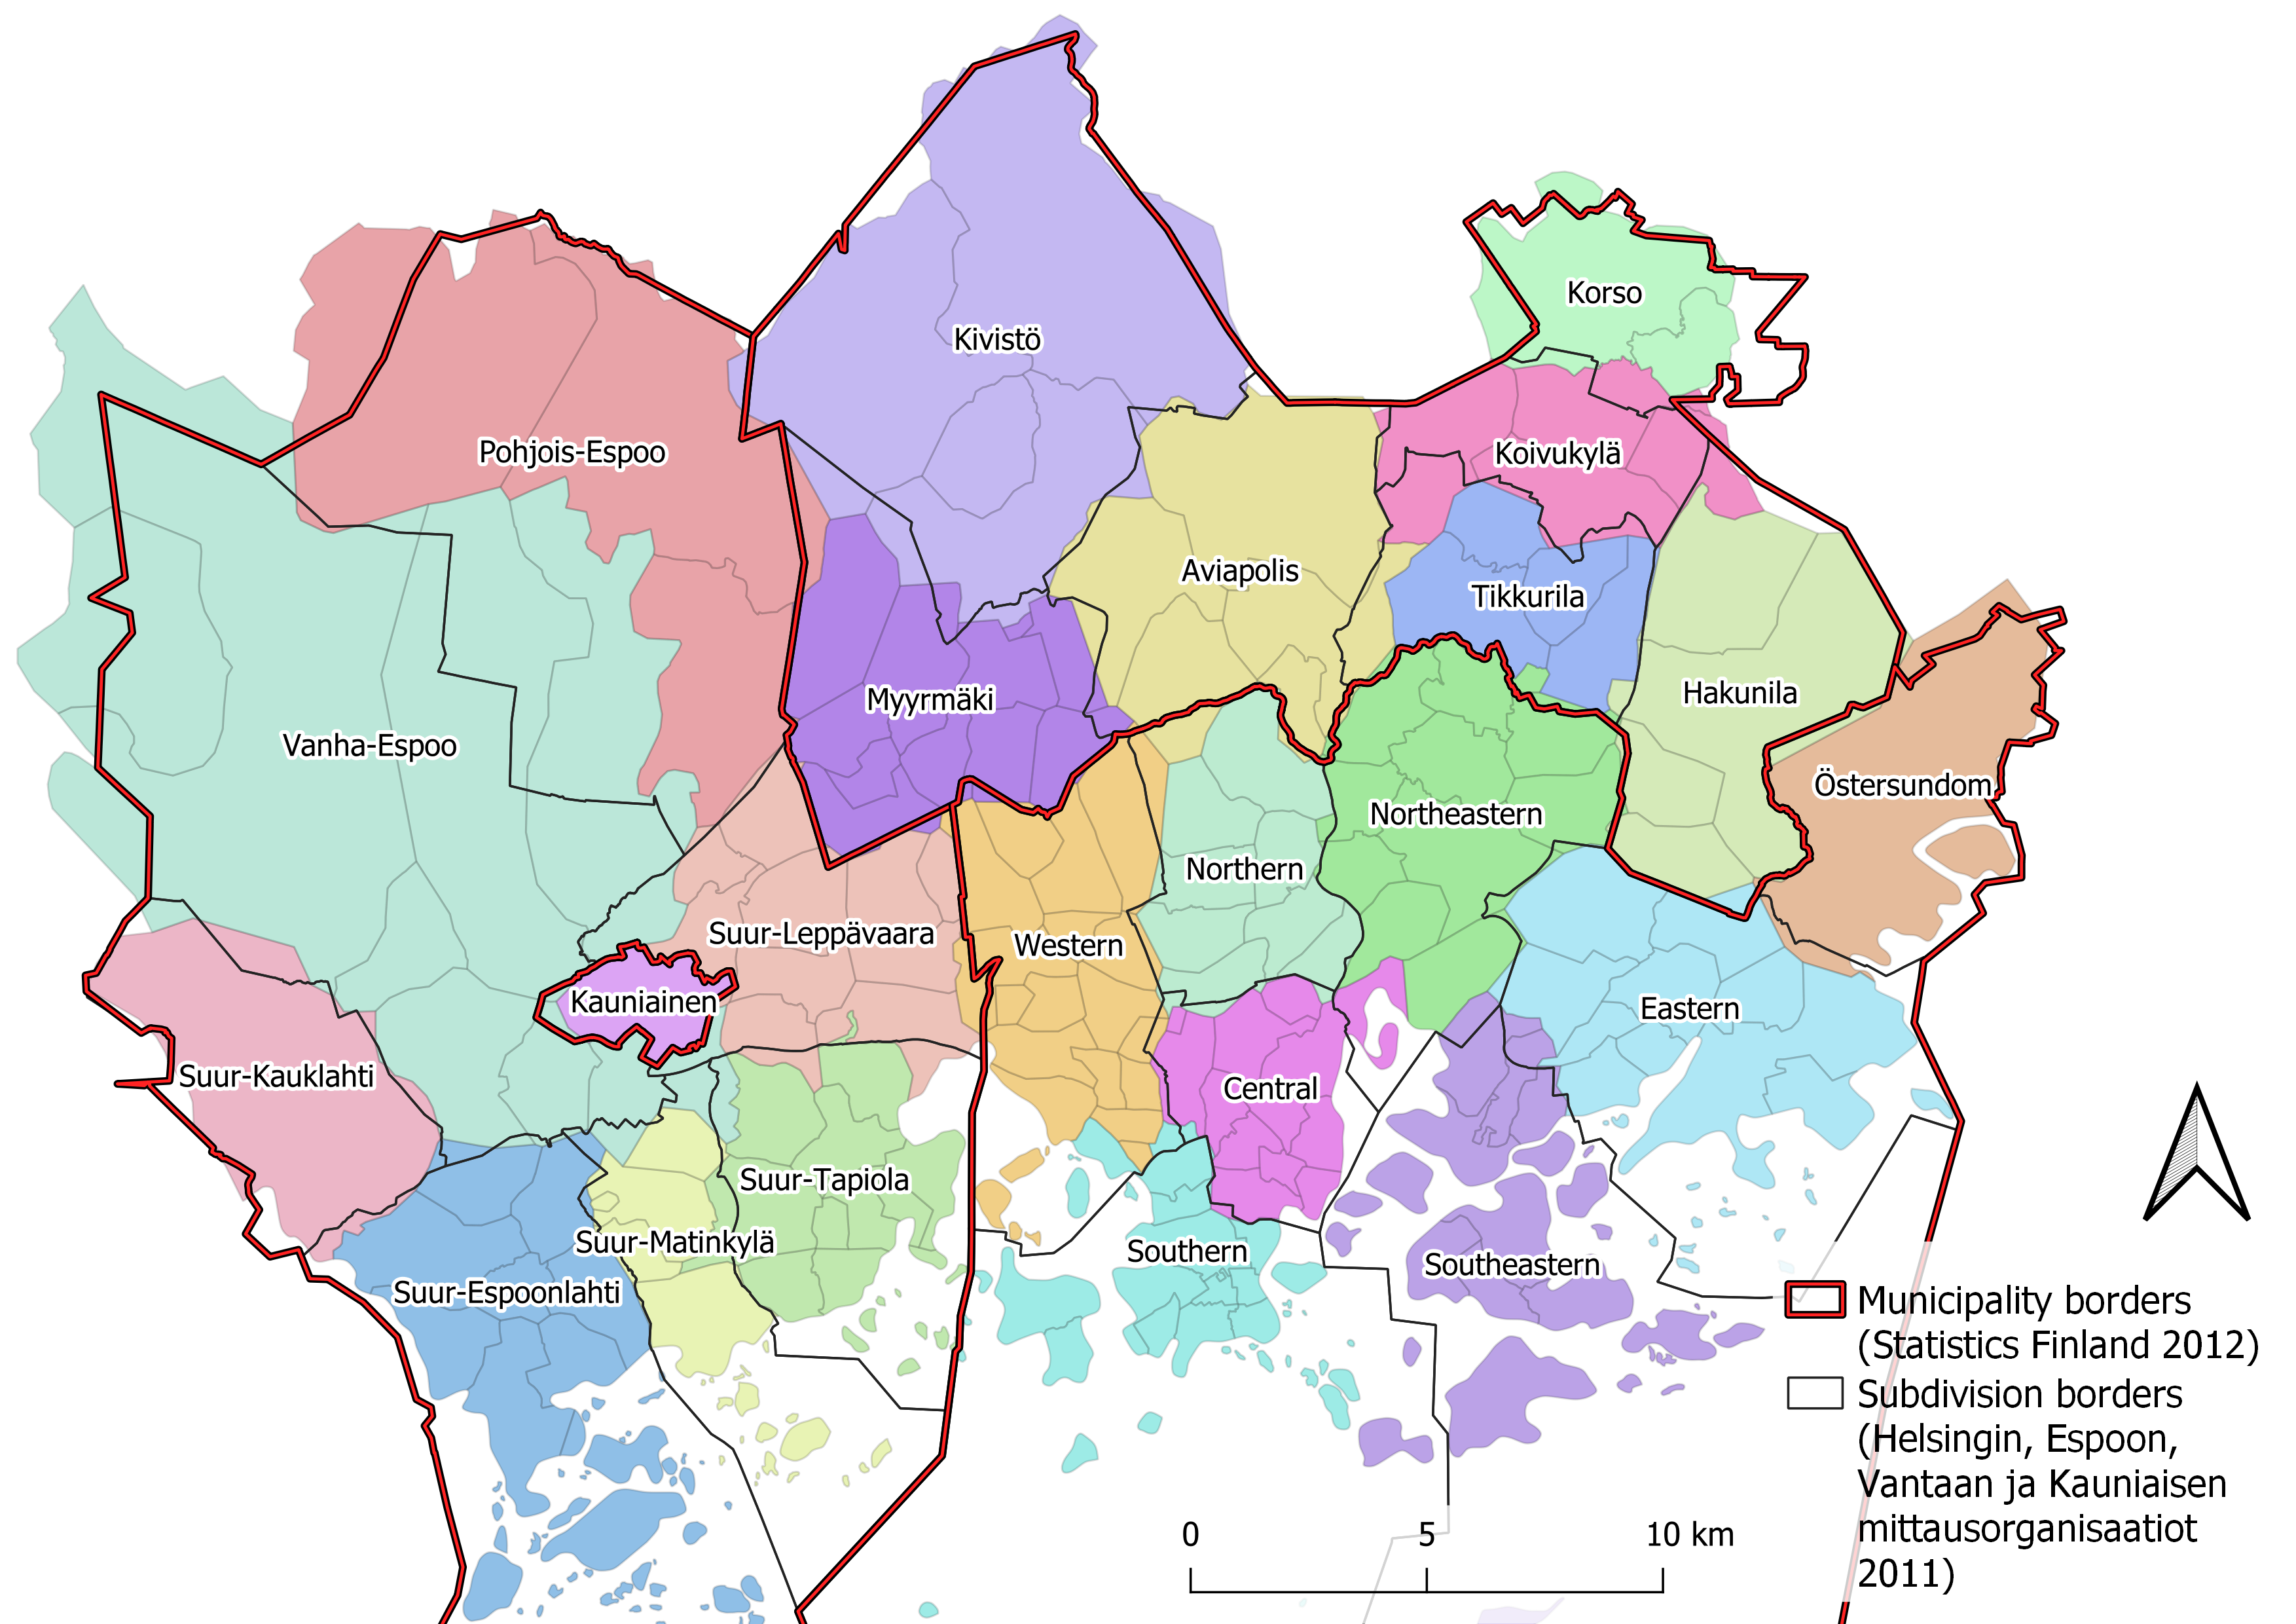
\includegraphics[width=\textwidth]{images/thesis_subdiv_place.png}
    \caption[Placing postal code areas in subdivisions]{For the purposes of analysis in R, all postal code areas in \textit{postal} were assigned with subdivision information. In this figure, distinct colors depict the postal code areas with the subdivision classification chosen for this thesis.}%
    \label{fig:subdiv_placement}%
\end{figure}

\newpage
\subsection{Creating applications and conducting analyses}
\subsubsection{Analysis application}
\justify
%\begin{itemize}
%    \item Prepare data to R compliant format
%    \item ShinyApp descriptive statistics
%    \item shinyapp histogram for parktime and walktime
%    \item shinyapp boxplot, show outliers
%    \item shinyapp barplot, show amounts
%    \item shinyapp levene test
%    \item shinyapp one-way anova
%    \item shinyapp map, nice to have, not at all important
%    \item visitor shinyapp, see the accumulation of visits and received records
%\end{itemize}

Once the data processing in Python was completed, \textit{records} and \textit{visitors} were carried over to R to utilise its easy to access statistical analysis functionality. For this thesis, this meant namely packages \textit{onewaytests} for ANOVA and Brown-Forsythe test, \textit{plotrix} for standard error, and \textit{moments} for quantiles (table~\ref{tab:used_soft}). To help study the large datasets, three Shiny applications were written, one for \textit{records} and a second for \textit{visitors}, and a third one to study differences between the thesis survey results and Helsinki Region Travel Time Matrix 2018. Benefits in creating these applications were twofold. Firstly, approaching the survey results from an interactive perspective allowed countless combinations of active and inactive variables -- without constant tweaking of code -- which would be beneficial for the analysis of \textit{records}. Secondly, programming the applications using Shiny enabled the use of shinyapps.io, a service where one can host Shiny applications on the internet without charge. Combination of these two factors made it effortless to analyse results of the survey in a visual way and at the same time, publish the tools and results to the public, upholding the thesis' mission of openness and transparency.

\begin{figure}[H]%
    \centering
    \subfloat[A segment of the shinyapps.io deployment of \textit{records} application. The web application provides a wide array of analysis and visualisation tools for the results of the thesis survey research.]{{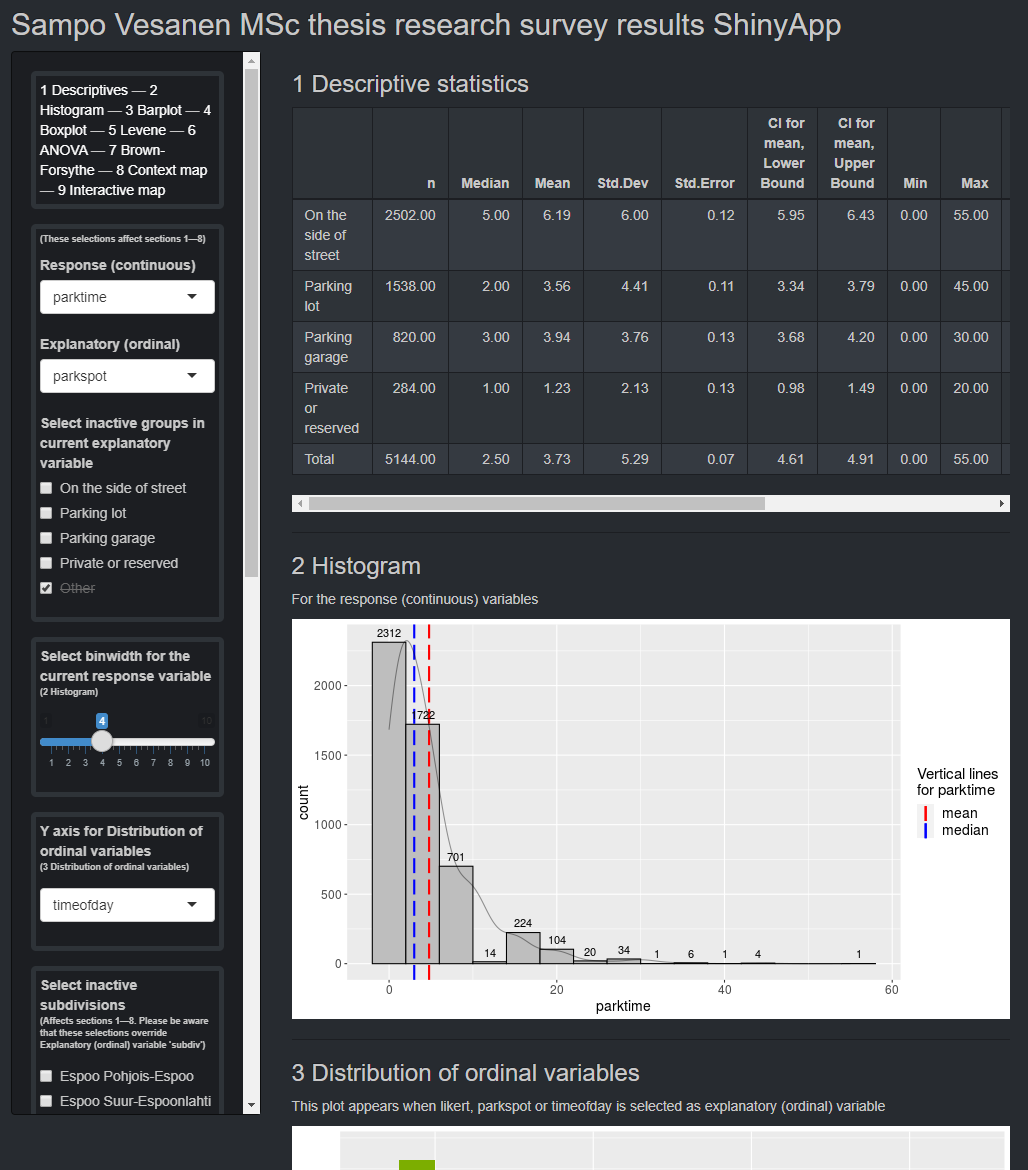
\includegraphics[width=8.1cm]{images/shinyapps_analysis.png} }}%
    \quad
    \subfloat[The shinyapps.io deployment of \textit{visitors} application. In this web application users may examine how the amounts of submitted responses and unique first visits to the thesis web survey developed over time.]{{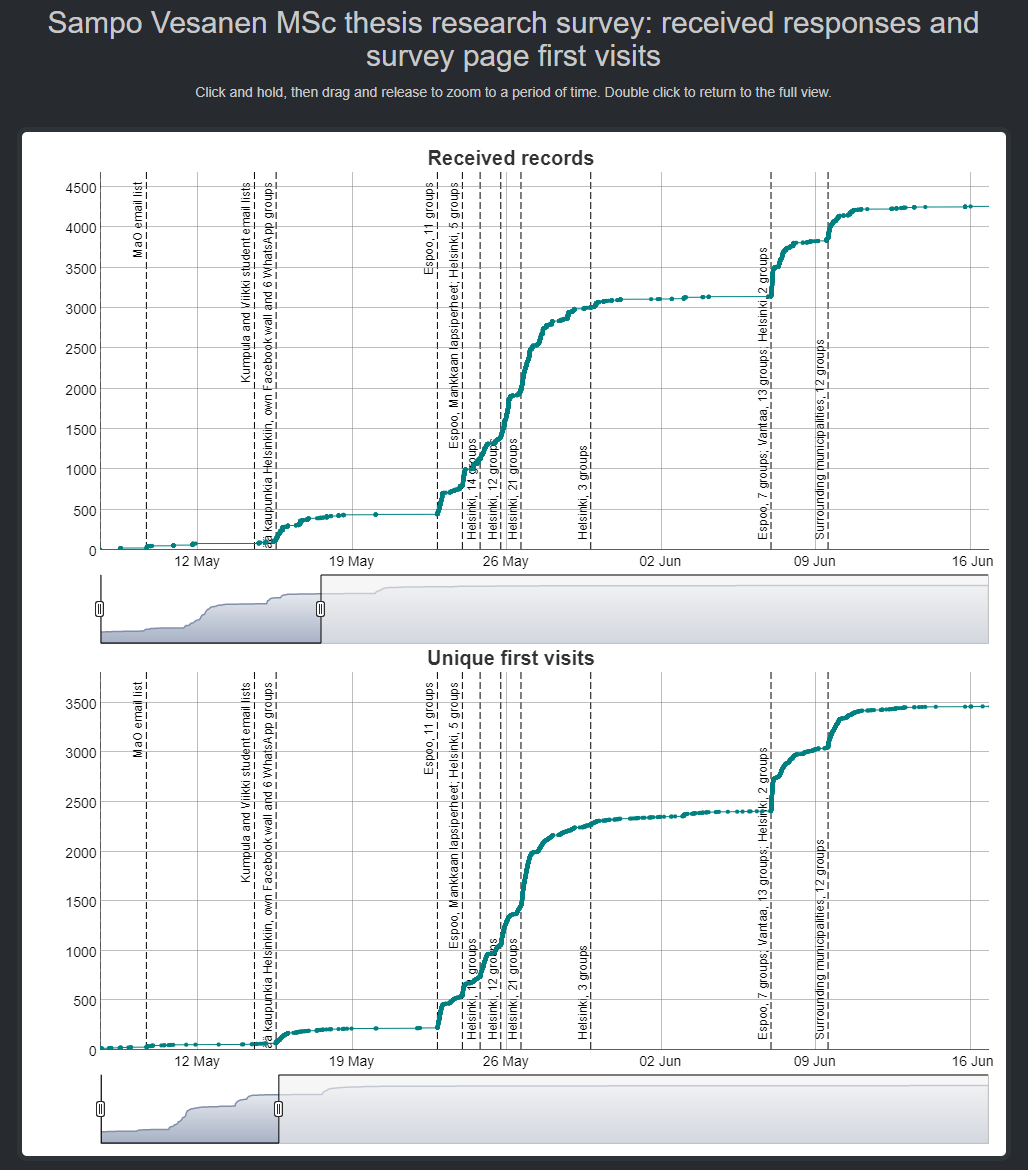
\includegraphics[width=8.1cm]{images/shinyapps_visitors.png} }}%
    \caption[Survey results as shinyapps.io web applications]{shinyapps.io deployments of the two survey dataset analysis applications.}%
    \label{fig:shinyapps}%
\end{figure}

In the Shiny application for \textit{records}, users can view the survey responses from many different angles. Users are given control which variables are active at any moment (\hyperref[fig:shinyapps]{figure~\ref{fig:shinyapps}a}). Users control the variables through the side panel, with settings taking effect in the main panel. The variables currently viewed are selected through two dropdown menus, Response (continuous) and Explanatory (ordinal). Continuous variables are \code{parktime} and \code{walktime} with an integer range 0--99. Available ordinal variables are \code{likert}, \code{parkspot}, \code{timeofday}, \code{artificial}, \code{ykr\_zone}, and \code{subdiv} with the values that can not be unequivocally ordered in a sequence in the same way as continuous variables. One variable from each variable group can be selected at the same time. Any and all groups of values in the ordinal variables can be deactivated to better understand the significance of each value group. In addition to the selection of the continuous and ordinal variable, users can deactivate \textit{records} data rows based on their spatial location in municipality subdivisions assigned in \hyperref[sec:processdata]{\fullref{sec:processdata}}. Most importantly, the analysis application allows selection of maximum allowed value for \code{parktime} and \code{walktime}. The default value for both is set at 59 minutes, as discussed in the \fullref{sec:processdata}, but the user is free to choose any value between zero and 99.

% levene, anova, boxplot, lue: https://www.itl.nist.gov/div898/handbook/eda/section3/eda35a.htm. On legit lähde
\begin{table}[H]
    \centering
    \caption[Records Shiny application features]{\textit{Records} Shiny application features. All features are affected by the maximum permitted \code{parktime} and \code{walktime} values, currently active response and explanatory variables and inactive subdivisions. In addition, certain exclusive settings are found in some of the features.}
    \label{tab:records_shiny_features}
    \scalebox{0.8}
    {\def\arraystretch{1.3}
    \setlength\tabcolsep{1.2ex}
    \begin{tabular}{ @{} >{\raggedright\arraybackslash}p{3cm} >{\raggedright\arraybackslash}p{2cm} >{\raggedright\arraybackslash}p{6cm} >{\raggedright\arraybackslash}p{6cm} @{} }
        \toprule
        Feature & Type & Outputs & Feature exclusive settings \\
        \midrule
        1 Descriptive statistics & Analysis, table & n, median, mean, standard deviation, standard error, confidence interval for mean, lower bound, confidence interval for mean, min, max, 25th quartile, 75th quartile, skewness, kurtosis & None \\
        2 Histogram & Analysis, chart & Histogram, kernel density estimate, mean, median & Histogram binwidth \\
        3 Distribution of ordinal variables & Analysis, chart & Distribution plot by explanatory variable value group & Explanatory variable for the distribution plot Y axis \\
        4 Boxplot & Analysis, chart & Quartile data & None \\
        5 Test of homogeneity of variances (Levene's test) & Analysis, table & Equality of variances for a variable calculated for the currently active response and explanatory variable & None \\
        6 Analysis of variance (ANOVA) & Analysis, table & Analysis of differences among group means in a sample & None \\
        7 Brown-Forsythe test & Analysis, table & Analysis of equality of group variances & None \\
        8 Interactive map & Visualisation, map & Choropleth map with Jenks breaks classifiction, descriptive data per postal code area (answer count, mean and median for parktime and walktime, forest amount percentage, largest YKR zone percentage) & - Selection of active municipalities \linebreak - Jenks breaks parameter column \linebreak - Amount of Jenks breaks classes \linebreak - Possibility to visualise the map with boundaries and labels \\
        \bottomrule
    \end{tabular}}
\end{table} 

When the user has selected a continuous and an ordinal variable to compare, they are presented a thorough set of descriptive statistics for the currently active data rows with n, median, mean, standard deviation, standard error, confidence interval for lower and upper bound, minimum and maximum, 25 \% and 75 \% quantiles, skewness, and kurtosis (table~\ref{tab:records_shiny_features}). For the continuous variables, a histogram is available to visualise the distribution of \code{walktime} and \code{parktime}. Distribution of ordinal variables \code{likert}, \code{parkspot}, and \code{timeofday} can be compared against other ordinal variables in a barplot. To study quartiles, a boxplot is available. Importantly, users can test their selection of variables with the test of homogeneity of variables (Levene's test), analysis of variance (ANOVA), and the Brown-Forsythe test \textcolor{red}{laajenna selityksiä}. Lastly, a versatile interactive map of the research area is provided. This map, divided in postal code areas, reveals the survey results in a spatial fashion. The interactive map is affected by the maximum parking time and walking time, selection of an ordinal variable and any inactive subdivisions to provide a flexible view into the details of the data. In addition, this interactive map is controlled by some exclusive settings of its own. The interactive map settings offers six distinct parameters for viewing the research area through Jenks natural breaks classification, alongside with the possibility to select the amount of classes in the map view. Hovering the cursor over the map reveals a tooltip which the application users can use to view mean, median, and percentage data about each postal code area in Helsinki Capital Region. Tooltips are also available for the barplot of distribution of ordinal variables and the boxplot.

Much additional work was put into the analysis application to make it as clear and easy to use as possible. The application features a number of links to move between the features and the settings, while smooth scrolling and animations help in directing the attention of the user. Each application feature can be switched on and off to make space for exactly the topic the user wants to examine. The analysis application allows downloading all the results, outputting tables into comma separated value files (CSV). Charts and the map are outputted into high resolution images (PNG). \textcolor{red}{too much detail?} \textcolor{purple}{The files are intuitively named informing of the used application settings and the date of file download. In case ordinal variable value groups or subdivisions are turned off, the output images are appended with an appropriate notification.} Attention was given to ensure the usage of the analysis application on mobile phones. To this end, the CSS style sheet of the application detects mobile phone screen sizes and adjusts the application content accordingly. The sidebar tends to block the view of the main panel on mobile screens and for this situation a switch is provided to hide the sidebar at any given time. All graphical elements of the application are in SVG (Scalable Vector Graphics) format which supports effortless zooming without loss of detail.

The source code for the \textit{records} analysis application is available at GitHub (\textcolor{blue}{\url{https://github.com/sampoves/thesis-records-shinyapps}}). The application may be viewed on shinyapps.io (\textcolor{blue}{\url{https://sampoves.shinyapps.io/records}}).

\subsubsection{Visitors application}

In the Shiny application for \textit{visitors}, users can examine events in the timeline of the survey research (figure~\ref{fig:shinyapps}). In this interactive view, cumulative charts are presented for received survey responses and survey page first visits. The charts reveal the effect and importance of advertisement on actual received responses and survey traffic. While not completely verifiable, the significance of different sources of responses can be viewed in the application.

Compared to the other two analysis applications programmed for this thesis, the \textit{visitors} application is relatively simple in its function and features. The user controls the chart view with mouse clicks or dragging the cursor and no additional settings are provided.

The source code for the \textit{visitors} analysis application is available at GitHub (\textcolor{blue}{\url{https://github.com/sampoves/thesis-visitors-shinyapps}}). The application may be viewed on shinyapps.io (\textcolor{blue}{\url{https://sampoves.shinyapps.io/visitors}}).

\subsubsection{Travel time comparison application}

Despite potential for extensive analysis, the applications described in previous chapters do not provide means to study the third research question of this thesis:

\begin{displayquote}
III What is the significance of the parking process to the overall travel time?
\end{displayquote}

To answer this research question, an application to compare travel time datasets was programmed (figure~\ref{fig:shinyapps_comparison}). In this application, the user can view a variety of descriptive values calculated from Helsinki Region Travel Time Matrix 2018, the thesis survey data, and a dataset created by comparing the two other datasets. The user is given control a set of features, such as the travel times origin postal area code, a parameter to visualise on the map, and the amount of symbology classes. The map view can be customised with a number of visualisation options, such as visible regional boundaries and physical features (inland water, main roads), and options for the labelling of postal code areas.

It was decided that the basic spatial unit for the comparison application would be the PAAVO postal code area as the thesis survey results exist in that resolution. This decision necessitated extensive processing of \textit{TTM} data. Firstly, the application needed to be able to recalculate the map view as quickly as possible. Secondly, the original \textit{TTM} dataset is unwieldy to be used in its original format in a web application (data stored in uncompressed txt files, data scope much too detailed for the application). Thirdly, the hosting service shinyapps.io places technical limitations on the resource intensity of the application. For these three main reasons, the library fst (table~\ref{tab:used_soft}) was first used to convert the \textit{TTM} private car columns into the data format used by the library (table~\ref{tab:comparison_fst1}), and then using the dataset \textit{grid} preprocessed in Python to aggregate all \textit{TTM} grid cell values to the PAAVO postal code area level and writing the results using the optimised fst format (table~\ref{tab:comparison_fst2}). For data completeness, \textit{TTM} searching for parking (0.42 minutes) and walking to destination (2.0--2.5 minutes) data was added to these aggregated \textit{TTM} files. This aggregation method drastically reduced unnecessary processing, minimised disk space needed, and kept application memory footprint in manageable figures for the deployment to the internet. The other main dataset used in the comparison application, the thesis survey data, is aggregated to postal code area level each time the application initialises, as the complete survey results dataset is miniscule in size compared to \textit{TTM}.

\begin{hyphenrules}{nohyphenation}
    \begin{table}[H]
        \centering
        \setlength\tabcolsep{1pt}
        \caption[Comparison application fst structure I]{An excerpt of the data content of \textit{TTM} converted to fst format for further processing (table~\ref{tab:comparison_fst2}). Original file 5785xxx/travel\_times\_to\_ 5785640.txt.} 
        \label{tab:comparison_fst1}
        \begin{tabular}{ @{} >{\raggedright\arraybackslash}p{1cm} >{\raggedright\arraybackslash}p{2cm} >{\raggedright\arraybackslash}p{2cm} >{\raggedright\arraybackslash}p{2cm} >{\raggedright\arraybackslash}p{2cm} >{\raggedright\arraybackslash}p{2cm} @{} }
            \toprule
            & from\_id & to\_id & car\_r\_t & car\_m\_t & car\_sl\_t \\
            \midrule
            10 & 5787549 & 5785640 & 22 & 21 & 16 \\
            11 & 5787550 & 5785640 & 22 & 21 & 16 \\
            12 & 5789447 & 5785640 & 10 & 9 & 8 \\
            13 & 5789448 & 5785640 & 10 & 9 & 8 \\
            14 & 5789449 & 5785640 & 11 & 10 & 9 \\
            \bottomrule
        \end{tabular}
    \end{table} 
\end{hyphenrules}

\begin{hyphenrules}{nohyphenation}
    \begin{table}[H]
        \centering
        \setlength\tabcolsep{5pt}
        \caption[Comparison application fst structure II]{An excerpt of the data content of \textit{TTM} aggregated to postal code area level for the use of the comparison application. The origin postal code area of the shown data table is 00100 Helsinki Keskusta -- Etu-Töölö.} 
        \label{tab:comparison_fst2}
        \begin{tabular}{ @{} >{\raggedright\arraybackslash}p{1cm} >{\raggedright\arraybackslash}p{1.5cm} >{\raggedright\arraybackslash}p{1.5cm} >{\raggedright\arraybackslash}p{2cm} >{\raggedright\arraybackslash}p{2cm} >{\raggedright\arraybackslash}p{2cm} >{\raggedright\arraybackslash}p{2cm} >{\raggedright\arraybackslash}p{2cm} @{} }
            \toprule
            & zipcode & from\_zip & ttm\_r\_avg & ttm\_m\_avg & ttm\_sl\_avg & ttm\_wtd & ttm\_sfp \\
            \midrule
            5 & 00150 & 00100 & 14.89 & 13.24 & 9.48 & 2.33 & 0.42 \\
            6 & 00160 & 00100 & 15.48 & 13.97 & 9.77 & 2.50 & 0.42 \\
            7 & 00170 & 00100 & 14.41 & 13.10 & 9.09 & 2.50 & 0.42 \\
            8 & 00180 & 00100 & 12.77 & 11.34 & 8.40 & 2.50 & 0.42 \\
            9 & 00190 & 00100 & 24.27 & 22.31 & 17.04 & 2.00 & 0.42 \\
            \bottomrule
        \end{tabular}
    \end{table} 
\end{hyphenrules}

\begin{hyphenrules}{nohyphenation}
    \begin{table}[H]
        \centering
        \setlength\tabcolsep{5pt}
        \caption[Comparison application tooltip content]{Comparison application tooltip content meaning.} 
        \label{tab:comparison_tooltip_content}
        \scalebox{0.85}
        {\begin{tabular}{ @{} >{\raggedright\arraybackslash}p{2cm} >{\raggedright\arraybackslash}p{2cm} >{\raggedright\arraybackslash}p{8.5cm} >{\raggedright\arraybackslash}p{5cm} @{} }
            \toprule
            & Column name & Description & Formula \\
            \midrule
            \multirow{3}{3cm}[-1ex]{timeofday} & r & Rush hour traffic (09:00–11.00, 15.00–17.00) & -- \\
            & m & Midday traffic (09.00–15.00) & -- \\
            & all & An average of all available data. For TTM18, these are Rush hour traffic, Midday traffic, and Route following speed limits without any additional impedances. For thesis survey data, these are the values of the survey question timeofday: Weekday, rush hour, Weekday, other than rush hour, Weekend, and Can't specify, no usual time. & -- \\
            \greyrule
            \multirow{5}{3cm}[-1ex]{Travel Time Matrix 2018} & sfp & Time consumed in searching for parking. In TTM18, this is 0.42 minutes for all YKR IDs (in the case of this application, postal code areas) in the entirety of Helsinki Capital Region (Toivonen et al. 2014). & -- \\
            & wtd\_avg & An averaged value (per postal code area, unit minutes) of walking time from one's parked private car to the final destination of the travel chain. In TTM18 this is 2.0 minutes for all YKR IDs in the entirety of Helsinki Capital Region, except in a square defined over the center of Helsinki, where the value is 2.5 minutes for all YKR IDs (Toivonen et al. 2014). See the switch "Helsinki walking center (TTM18)" in the toolbar to the left. & -- \\
            & avg & A mean duration (per postal code area, unit minutes) of the complete travel chain with private car from origin postal code area to the destination postal code area. & car\_x\_t1 + car\_x\_t2 + ... + car\_x\_tn / n, where x is r, m, or all. car\_ represents unchanged TTM18 data columns. \\
            & drivetime & The length of the driving segment (unit minutes) of the mean duration of the complete travel chain from origin postal code area to the destination postal code area without searching for parking (using the TTM18 value) or walking to the final destination of the travel chain (TTM18 value). & ttm\_x\_avg - ttm\_sfp - ttm\_wtd\_avg, where x is r, m, or all. \\
            & pct & How much does searching for parking and walking from one's parked car to the final destination of the travel chain constitute of the mean duration of the complete travel chain? Value per postal code area, unit percent, where 1 equals 100 \%. & (ttm\_sfp + ttm\_wtd\_avg) / ttm\_x\_avg, where x is r, m, or all. \\
            \greyrule
            \multirow{4}{3cm}[-1ex]{Thesis data} & sfp\_avg & Time consumed, on average, in searching for parking in a postal code area, according to the thesis survey respondents. The thesis data variable parktime was averaged for the current postal code area for the use of this application. & parktime1 + parktime2 + ... + parktimen / n, while postal code value is constant. \\
            & wtd\_avg & Average walking time from one's parked private car to the final destination in a postal code area, according to the thesis survey respondents. The thesis data variable walktime was averaged for the current postal code area for the of this application. & walktime1 + walktime2 + ... + walktimen / n, while postal code value is constant. \\
            & drivetime & The length of the driving segment (value per postal code area, unit minutes) of the mean duration of the complete travel chain (TTM18 data) from the origin postal code area to the destination postal code area, without searching for parking (thesis survey mean) or walking to destination (thesis survey mean). & ttm\_x\_avg - thesis\_x\_sfp - thesis\_x\_wtd, where x is r, m, or all. \\
            & pct & How much do the thesis mean values for searching for parking and walking from one's parked car to the final destination constitute of the mean duration of the complete travel chain (calculated from TTM18 data)? Value per postal code area, unit percent, where 1 equals 100 \%. & (thesis\_x\_sfp + thesis\_x\_wtd) / ttm\_x\_avg, where x is r, m, or all. \\
            \greyrule
            \multirow{4}{3cm}[-1ex]{Compare TTM and thesis} & sfp & Compare TTM18 and thesis survey values for searching for parking. If this comparison value is smaller than one, searching for parking takes longer in TTM18. If value is larger than one, searching for parking takes longer in thesis data. & thesis\_x\_sfp / ttm\_sfp, where x is r, m, or all. \\
            & wtd & Compare TTM18 and thesis survey values for the duration to walk from one's parked car to the final destination of the travel chain. & thesis\_x\_wtd / ttm\_wtd\_avg, where x is r, m, or all. \\
            & drivetime & Compare the driving time segment of the mean duration of the complete travel chain in TTM18 and thesis data. & thesis\_x\_drivetime / ttm\_x\_drivetime, where x is r, m, or all. \\
            & pct & Compare the percentual value of the significance of searching for parking and walking to one's final destination of the mean duration of the complete travel chain in TTM18 and thesis data. & thesis\_x\_pct / ttm\_x\_pct, where x is r, m, or all. \\
            \bottomrule
        \end{tabular}}
    \end{table} 
\end{hyphenrules}

\begin{figure}[H]%
    \centering
    \includegraphics[width=0.33\textwidth]{images/shinyapps_comparison_detail.png}
    \caption[Comparison application data]{Close-up of a tooltip for a travel chain from 02150 Otaniemi to 02170 Haukilahti. The cell coloured green tells the user that currently visualised on map is thesis data, the travel chain without searching for parking or walking to one's destination, in rush hour traffic.}%
    \label{fig:shinyapps_comparison_detail}%
\end{figure}

\begin{figure}[H]%
    \includegraphics[width=\textwidth]{images/shinyapps_comparison.png}
    \caption[Comparison application screenshot]{Helsinki Region Travel Time Matrix 2018 and thesis survey data comparison application's shinyapps.io deployment. The cursor hovers over 01200 Hakunila with the appropriate tooltip shown.}%
    \label{fig:shinyapps_comparison}%
\end{figure}

The source code for the travel time comparison application is available at GitHub (\textcolor{blue}{\url{https://github.com/sampoves/thesis-comparison-shinyapps}}). The application may be viewed on shinyapps.io (\textcolor{blue}{\url{https://sampoves.shinyapps.io/comparison}}).
\import{content/}{c3_data.tex}%
% EN TAJUU; JOS C3_DATAN TUO TÄHÄN; EI TUU SOMETHING'S WRONG -ERRORIA
% EHKÄ EN VAAN VÄLITÄ NOISTA ERROREISTA, PITÄISKÖ OLLA VÄLITTÄMÄTTÄ?

% RESULTS
\newpage
\section{Results}
\subsection{Survey results in summary}
\justify

%- Present results in the order of the research questions
%- (Amount of records, amount of faulty records)
%- Uncertainties
%- Present logically all results and interesting specific questions
%- Compare parking with original Travel Time Matrix values and values collected by me
%- Charts, statistics
%- Just show your findings, no nonsense
In this chapter, the thesis research survey results which fit the criteria as per shown in \hyperref[sec:processdata]{\fullref{sec:processdata}} is discussed. Within the selected criteria (\code{parktime < 60} and \code{walktime < 60}), the survey received a total of 5579 visits from 4320 unique IP addresses. 848 unique IP addresses visited the survey more than one time and in total 1060 unique IP addresses sent data to the survey. 24.5 percent of all visitors submitted at least one data row. On average one respondent submitted 4.9 data rows.

The survey received in total 5183 data rows. All postal code areas were represented in the survey results (figure~\ref{fig:postalvis_answers}), but the data row count histogram was heavily skewed to the right, with the first quartile being eight data rows, second (median) 17 data rows and third 42 data rows (table~\ref{tab:muns_answer_stats}, figures~\ref{fig:parktime_hist},~\ref{fig:walktime_hist}). Most respondents reported short parking times below ten minutes, but the histograms do not smoothly lessen in values from the right to left, as people have preferred to report round figures such as five, ten, or fifteen minutes. There were five postal code areas with more than one hundred data rows and 55 postal code areas with less than ten data rows. In Helsinki, the answers strongly clustered around the center of Helsinki, with other centers of activity being Herttoniemi and Itäkeskus-Marjaniemi in Helsinki, Tapiola-Otaniemi and Leppävaara in Espoo, and Tikkurila-Vantaanportti in Vantaa.

\begin{figure}[H]%
    \centering
    \includegraphics[width=\textwidth]{images/hist_pmax59-wmax59_parktime-likert_binw2_02-08-2020.png}
    \caption[Histogram, searching for parking]{All permitted thesis survey \code{parktime} values (< 60) shown on histogram.}%
    \label{fig:parktime_hist}%
\end{figure}

\begin{figure}[H]%
    \centering
    \includegraphics[width=\textwidth]{images/hist_pmax59-wmax59_walktime-likert_binw2_02-08-2020.png}
    \caption[Histogram, walk to destination]{All permitted thesis survey \code{walktime} values (< 60) shown on histogram.}%
    \label{fig:walktime_hist}%
\end{figure}

\begin{hyphenrules}{nohyphenation}
    \begin{table}[H]
        \centering
        \def\arraystretch{1.2}
        \setlength\tabcolsep{4pt}
        \caption[Answer counts by municipality]{Amount of data rows received per municipality in Helsinki Capital Region.} 
        \label{tab:muns_answer_stats}
        \begin{tabular}{ @{} >{\raggedright\arraybackslash}p{3cm} >{\raggedright\arraybackslash}p{2cm} >{\raggedright\arraybackslash}p{4cm} >{\raggedright\arraybackslash}p{2cm} >{\raggedright\arraybackslash}p{2cm} @{} }
            \toprule
            Municipality & Data rows total & Most data rows in municipality & Data rows mean in municipality & Data rows median in municipality \\
            \midrule
            Helsinki & 3777 & 271 (00100 Helsinki Keskusta - Etu-Töölö) & 45.0 & 34.5 \\
            Espoo & 637 & 84 (02600 Etelä-Leppävaara) & 17.7 & 9 \\
            Vantaa & 746 & 91 (01510 Kirkonkylä-Veromäki) & 16.2 & 8 \\
            Kauniainen & 23 & 23 (02700 Kauniainen) & 23 & 23 \\
            % use \usepackage[table]{xcolor} and \usepackage{booktabs} to define \greyrule
            \greyrule
            All & 5183 & 271 (00100 Helsinki Keskusta - Etu-Töölö) & 31.0 & 17 \\
            \bottomrule
        \end{tabular}
    \end{table} 
\end{hyphenrules}

On a closer look to the municipalities, finer details become apparent (figure~\ref{fig:postalvis_answers}). For example, in Helsinki, a wedge-like area of survey activity in the direction of southwest-northeast is visible. Starting out from the west, this area spans from Lauttasaari to the center of Helsinki and moving on all the way east to Malmi. Many of the areas which could be roughly characterised as residential areas were left with little activity. Furthermore, in the survey instructions respondents were requested to refrain from including parking activity in private property, as it was assumed in survey design phase that these areas would provide near to instantaneous parking, potentially distorting the data and obfuscating the objectives set by the thesis research questions. The lightness of activity in residential areas corresponds with the made request.

% A known issue with these maps: Vartiosaari is represented on these maps. As an unreachable island, it shouldn't.
\begin{figure}[H]%
    \centering
    \includegraphics[width=\textwidth]{images/thesis_postalvis_answers.png}
    \caption[Data rows received per postal code area]{This figure illustrates the responses received in the thesis survey per postal code area (n=167). Classes are in natural breaks (Jenks). Municipality borders are based on \textit{postal} data. There are slight differences to the actual municipality boundaries.}%
    \label{fig:postalvis_answers}%
\end{figure}

In the finest resolution available, the postal code areas, long \code{parktime} values closely follow areas with most survey activity (table~\ref{fig:postalvis_parkmean}, table~\ref{fig:postalvis_parkmedian}). The longest \code{parktime} values were encountered in the center of Helsinki, where the mean value for 00120 Punavuori was 10.6 minutes (median 10.0 minutes, 91 data rows) and 00290 Meilahden sairaala-alue 9.4 minutes (5.0 min, 42 data rows). Long parking times over five minutes were recorded in all over the center area, but also in 00570 Kulosaari (mean 5.3 minutes, median 5.0 minutes, 48 data rows) and 00590 Kaitalahti (6.5 min, 3.5 min, 16 data rows). In Espoo, the longest \code{parktime} values were found in 02230 Matinkylä (5.1 min, 5.0 min, 62 data rows), 02100 Tapiola (4.6 min, 3.0 min, 71 data rows), and in 02320 Espoonlahti (4.3 min, 3.0 min, 30 data rows). In Vantaa, it took the longest to find a parking spot in 01300 Tikkurila with (6.4 min, 5.0 min, 85 data rows). According to the survey results, it was relatively hard to find a parking spot in 01700 Kivistö (5.7 min, 4.0 min, 30 data rows), too.

In the case of this survey dataset it is important to not lose sight of median, as mean is susceptible to outliers, of which there are many present. One such situation may be viewed in 01750 Keimola, where the mean \code{parktime} is 5.9 minutes, and median reads at 1.0 minute. In Keimola's situation, one respondent entered a \code{parktime} value of 25 minutes, severely skewing the total sample of seven values. It may be argued that when detecting areas of long duration of searching for parking, median is the better measure to identify areas of interest.

The mean \code{walktime} values follow the same municipal order as those of \code{parktime}: On average, in Helsinki it took 4.8 minutes to walk from one's parked car to the final destination of the journey (table~\ref{fig:postalvis_walkmean}, table~\ref{fig:postalvis_walkmedian}). In Vantaa, this process was 4.0 minutes, while Espoo had mean parking time of 3.9 minutes and Kauniainen 2.2 minutes. Viewing median values, this is 4.0, 3.0, 2.0, and 2.0 minutes for Helsinki, Vantaa, Espoo, and Kauniainen, respectively. Of the entire research area, Espoo's 02780 Kauklahti stood out with a mean walking time of 6.3 minutes (median 5.5 min) to one's destination. It is notable that this subdivision received 10 answers, ranking second to the last before Helsinki's 00890 Östersundom's total of 6 answers.

When viewed through postal code areas, \code{walktime} shows the longest durations to walk from one's car to the final destination in Helsinki with the top belonging to 00100 Helsinki Keskusta -- Etu-Töölö (mean 7.4 minutes, median 5.0 minutes, 271 data rows). Most of the central Helsinki did not fall far behind with most values ranging from five to seven minutes. Outside of the center of Helsinki, 00570 Kulosaari (6.7 min, 5.0 min, 48 data rows), 00590 Kaitalahti (6.3 min, 5.0 min, 16 data rows) and 00690 Tuomarinkylä-Torpparinmäki (5.3 min, 3.0 min, 15 data rows) saw long \code{walktime} values within the boundaries of Helsinki. Looking outward from the capital, the \code{walktime} values in Espoo were mostly lower than those in Helsinki. Longest recorded durations in Espoo were in 02100 Tapiola (5.4 min, 5.0 min, 71 data rows), 02780 Kauklahti (6.3 min, 5.5 min, 10 data rows), and 02820 Nupuri-Nuuksio (7.0 min, 5.0 min, 7 data rows). Vantaa's longest \code{walktime} values were found in 01530 Veromiehenkylä (8.0 min, 5.5 min, 48 data rows), 01300 Tikkurila (6.3 min, 5.0 min, 85 data rows), and 01700 Kivistö (5.6 min, 5.0 min, 30 data rows). 

It is difficult to try and determine the causes behind these long \code{walktime} values, but it may be worth noting, that many of the postal code areas with top values contain popular sightseeing locations, such as the Haltiala domestic animal farm in 00690 Tuomarinkylä-Torpparinmäki and the national park of Nuuksio in 02820 Nupuri-Nuuksio. The postal code area of 01530 Veromiehenkylä is almost entirely in the use of Helsinki-Vantaa Airport. It quickly becomes apparent that recreational trips to Nuuksio National Park may nudge the Espoo's \code{walktime} values upward, while in Vantaa, the Helsinki-Vantaa Airport walking seems to be a similar factor. A summarising feature about \code{walktime} is that areas of long walking times from one's car to the final destination are not as apparently clustered as those of \code{parktime} are.


\begin{figure}[H]%
    \centering
    \includegraphics[width=.88\textwidth]{images/thesis_postalvis_parkmean.png}
    \caption[Parktime, mean, in the reseach area]{This figure illustrates the mean duration of searching for parking and parking one's car in each postal code area.}%
    \label{fig:postalvis_parkmean}%
\end{figure}

\begin{figure}[H]%
    \centering
    \includegraphics[width=.88\textwidth]{images/thesis_postalvis_parkmedian.png}
    \caption[Parktime, median, in the reseach area]{This figure illustrates the median duration of searching for parking and parking one's car in each postal code area.}%
    \label{fig:postalvis_parkmedian}%
\end{figure}

\begin{figure}[H]%
    \centering
    \includegraphics[width=.88\textwidth]{images/thesis_postalvis_walkmean.png}
    \caption[Walktime, mean, in the research area]{This figure illustrates the mean duration of walking from one's parked car to the final destination in each postal code area.}%
    \label{fig:postalvis_walkmean}%
\end{figure}

\begin{figure}[H]%
    \centering
    \includegraphics[width=.88\textwidth]{images/thesis_postalvis_walkmedian.png}
    \caption[Walktime, median, in the research area]{This figure illustrates the median duration of walking from one's parked car to the final destination in each postal code area.}%
    \label{fig:postalvis_walkmedian}%
\end{figure}

\newpage
\subsection{Statistics}
\justify

The thesis survey data reveals that there are spatial differences between municipalities and regions of Helsinki Capital Region (table~\ref{tab:park_walk_subdiv}) in the durations to find a parking spot (\code{parktime}), and walking from one's parked car to the final destination (\code{walktime}). This is shown by the one-way analysis of variance test (ANOVA) that for \code{parktime} and \code{walktime} there are statistically significant differences ($p < 0.05$) between the 23 groups (municipality subdivisions, figure~\ref{fig:subdiv_placement}). In the vast majority of subdivision groups, the group sizes were sufficiently large for ANOVA analysis to be significant. An exception to this is the ANOVA test for Espoo's subdivisions using \code{parktime}. This test finishes with a less significant $p = 0.015$.

The spatial differences between subdivisions were wide-ranging, with a 5.2 minutes mean \code{parktime} in Helsinki, 3.8 minutes in Vantaa, 3.2 minutes in Espoo and lastly, 2.1 minutes in Kauniainen. Median \code{parktime} for the municipalities were 4.0, 2.0, 2.0, and 2.0 minutes, respectively. Durations to find a parking spot varied inside municipalities; in Espoo, in the subdivision of Pohjois-Espoo mean \code{parktime} was 1.7 minutes (median 1.0 minute) while the same value for Suur-Matinkylä was 4.3 minutes (3.0 min). From all the subdivisions in the research area, the subdivision representing the center of Helsinki, Helsinki Southern, had the the longest mean \code{parktime}, 7.3 minutes (5.0 min). Kauniainen ranked as fourth with a \code{parktime} values 2.1 minutes mean and 2.0 minutes median.

Viewing \code{walktime} through subdivisions, longest \code{walktime} was found from Espoo's Suur-Kauklahti (mean 6.3 min, median 5.5 min). In Helsinki, the Southern subdivision's durations were the second longest (mean 6.3 min, median 5.0 min) with Vantaa's top values reaching 5.8 minutes mean and 5.0 median in Tikkurila. Kauniainen's \code{walktime} values were more moderate with 2.2 minutes mean and 2.0 minutes median.

When comparing specific subdivisions, we can observe finer details in the survey dataset. For example, comparing \code{parktime} in Espoo's Suur-Tapiola and Vantaa's Aviapolis gives no statistical significance with ANOVA ($p = 0.12$). However, a test with Suur-Tapiola and Helsinki's Southern subdivision is statistically significant ($p < 0.05$). It is interesting, that an ANOVA \code{parktime} comparison of Espoo's Suur-Leppävaara and Helsinki's Northeastern subdivisions -- both important subcenters of their respective cities -- produces no statistical significance ($p = 0.84$). 

Differences of Espoo's Vanha-Espoo and Helsinki's Östersundom subdivisions viewed with \code{walktime} gives a faint statistical significance with ANOVA ('.', $p = 0.06$). Differences of Vanha-Espoo and Vantaa's Tikkurila proved not statistically significant (' ', $p = 0.20$). It is interesting that important city centers receive different results from the ANOVA test. For example, differences in \code{walktime} are statistically significant (’***’, $p \leq 0.001$) between Vantaa's Myyrmäki and Tikkurila subdivisions. \code{walktime} differences of Espoo's Suur-Matinkylä and Suur-Leppävaara are not (' ', $p = 0.13$). The same case stands for Helsinki's Southeastern and Western subdivisions of which differences were not identified as statistically significant (' ', $p = 0.76$). However, varying degrees of significance is found for the same subdivision comparison pairs when using \code{parktime} as the explanatory variable: Myyrmäki--Tikkurila achieves high statistical significance (’***’, $p \leq 0.001$), while Suur-Matinkylä--Suur-Leppävaara ('**', $p = 0.007$), and Southeastern--Western ('**', $p = 0.007$) get moderate significance.

% \textcolor{red}{290720 kun verrataan kahta subdiviä (2 ryhmää), käytetään anovaa ja katsotaan merkitsevyys. Suur-Tapiola ja Aviapolis oli " ", ei-merkitsevä, Suur-Tapiola ja Helsinki Southern ***. Kirjoita muutamasta parista, joissa ***. Vois mainita yhden kiinnostavan, missä parkkiaikojen ero on kohinaa (Tapiola ja Aviapolis). Muista tää sama walktimelle.} \\
% \textcolor{red}{290720 katso muut muuttujat niin, että mukana kaikki subdivit, onko merkitsevyyttä anovassa} \\
% \textcolor{red}{290720 parktime: verrataan arki-viikonloppu, **, walktime: ei ole ollenkaan!} \\
% \textcolor{red}{voi tutkii myös kaupunkien erot pareina, mutta tämä taitaa tarvita koodia} \\
% \textcolor{red}{parktime Espoossa ja Helsingissä (eri tarkastelut), espoossa ei niin väliä milloin pysäköi, kun taas helsingissä merkittävämmät erot} \\
% \textcolor{red}{raportoi nyt ne mun omatkin variaapelit!} \\
%\textcolor{red}{comparison-sovelluksen tulokset: muutama esimerkkireitti ja kerro pct:stä} \\
% 290720 vantaan timeofday arkiruuhka ja arkiei-ruuhka oudot tulokset, arkiruuhka nopeampi. Mutta tämä on ei-merkitsevä anovan mukaan! synninpäästö
% 290720 espoon timeofdayn pienet erot ovat kohinaa anovan mukaan (ei-merkitsevä), can't specify ei mukana
% 290720 anova kertoo että onks vähintään JOKU 1 ryhmä merkitsevästi eri kuin muut, sitten seuraavaksi pitäis tutkii lisää, vaikka pareittain



%https://www.researchgate.net/post/Is_there_a_minimum_number_per_group_neccessary_for_an_ANOVA
%anova - ryhmän koko anovassa
% interpret anova table in r
%http://www.understandingdata.net/2017/05/11/anova-tables-in-r/
%https://www.statisticssolutions.com/sample-size-calculation-for-one-way-anovas-in-dissertations-and-theses/

% levene näyttää vain vähän eri, niin ei oo välii, sitten pitäis kattoo keskihajontaa
%anova pitäis olla ok koska 20 tapausta jo riittävä tuloksen löytymiseen 
%voin todeta, että on tilastolliseti merkitsevä ero, sitten vaan raportoi mikä on ero, esim espoo vs helsinki
%anova todistaa, että kaikilla esim "subdiveillä" ei ole samoja arvoja
%-- parittaiset t-testit jos haluaa kahden paikan välillä testailla
%-- viikonloppuaikojen sisällä varianssi ja viikonpäivän varianssi, kuinka paljon varianssista se selittää
%-- power-analyysi?? Eta-squared (eta2)

%https://statistics.laerd.com/spss-tutorials/one-way-anova-using-spss-statistics-2.php
%LINKISTÄ: therefore, there is a statistically significant difference in the
%mean length of time to complete the spreadsheet problem between the different 
%courses taken.

\begin{hyphenrules}{nohyphenation}
    \begin{table}[H]
        \centering
        \caption[Parktime and walktime descriptive statistics with explanatory variable subdiv]{Parking times and walking times descriptive statistics displayed by municipalities and subdivisions (the explanatory variable \code{subdiv}). The unit of median, mean, and standard deviation is minutes. Significance codes: '***' $p \leq 0.001$, '**' $p \leq 0.01$, '*' $p \leq 0.05$, '.' $p \leq 0.1$, 'ns' $p \leq 1$.}
        \label{tab:park_walk_subdiv}
        \scalebox{0.66}
        % Column type C is a custom column which adds space to its position. Used to separate important features of this table. L aligns left.
        {\begin{tabular}{clLccccCcccccc}
            \toprule
		    & & &                                       \multicolumn{5}{c}{parktime} &          \multicolumn{5}{c}{walktime} \\
														\cmidrule(lr{\tbspace}){4-8}            \cmidrule(lr){9-13}
			& & n &                                     Median & Mean & Std.dev & Std.err & p-value & Median & Mean & Std.dev & Std.err & p-value \\
            
            \midrule
            \multirow{7}{*}{Espoo} & Pohjois-Espoo &    29 & 1 & 1.69 & 2.12 & 0.39 & &         1 & 1.86 & 1.55 & 0.29 & \\
            & Suur-Espoonlahti &                        99 & 2 & 2.88 & 3.27 & 0.33 & &         2 & 2.83 & 2.67 & 0.27 & \\
            & Suur-Kauklahti &                          10 & 2 & 3.50 & 3.69 & 1.17 & &         5.5 & 6.30 & 4.81 & 1.52 & \\
            & Suur-Leppävaara &                         176 & 2 & 3.12 & 2.94 & 0.22 & &        3 & 3.27 & 2.41 & 0.18 & \\
            & Suur-Matinkylä &                          95 & 3 & 4.28 & 4.05 & 0.42 & &         3 & 3.76 & 2.81 & 0.29 & \\
            & Suur-Tapiola &                            257 & 2 & 3.33 & 3.94 & 0.25 & &        2 & 3.84 & 3.41 & 0.21 & \\
            & Vanha-Espoo &                             80 & 2 & 2.81 & 4.00 & 0.45 & &         3 & 3.89 & 3.81 & 0.43 & \\
            % Use \arrayrulecolor to get a grey cmidrule, then revert \midrule color back to black
            \arrayrulecolor{black!30}\cmidrule(lr){2-13}
            & \textbf{Total} &                          746 & 2 & 3.23 & 3.63 & 0.13 & * &    2 & 3.52 & 3.09 & 0.11 & *** \\
            \arrayrulecolor{black}\midrule
            
            \multirow{8}{*}{Helsinki} & Central &       704 & 5 & 5.54 & 5.72 & 0.22 & &        5 & 4.91 & 3.92 & 0.15 & \\
            & Eastern &                                 360 & 2 & 3.61 & 3.41 & 0.18 & &        3 & 3.91 & 3.51 & 0.18 & \\
            & Northeastern &                            308 & 2 & 3.19 & 3.83 & 0.22 & &        3 & 3.63 & 3.47 & 0.20 & \\
            & Northern &                                162 & 1 & 2.38 & 2.73 & 0.21 & &        2 & 3.16 & 3.21 & 0.25 & \\
            & Southeastern &                            315 & 2 & 3.42 & 3.72 & 0.21 & &        2 & 3.70 & 3.79 & 0.21 & \\
            & Southern &	                            1310 & 5 & 7.26 & 6.47 & 0.18 & &       5 & 6.23 & 4.56 & 0.13 & \\
            & Western &                                 612 & 2 & 4.28 & 5.04 & 0.20 & &        3 & 3.63 & 3.15 & 0.13 & \\
            & Östersundom &                             6 & 0.5 & 0.67 & 0.82 & 0.33 & &        1 & 0.83 & 0.75 & 0.31 & \\
            \arrayrulecolor{black!30}\cmidrule(lr){2-13}
            & \textbf{Total} &                          3777 & 4 & 5.24 & 5.60 & 0.09 & *** &   4 & 4.78 & 4.10 & 0.07 & *** \\
            \arrayrulecolor{black}\midrule
            
            Kauniainen & Kauniainen &                   23 & 2 & 2.13 & 1.60 & 0.33 & --- &     2 & 2.22 & 1.28 & 0.27 & --- \\
            \midrule
            
            \multirow{7}{*}{Vantaa} & Aviapolis &       184 & 3 & 3.93 & 4.09 & 0.30 & &        3 & 4.51 & 4.27 & 0.31 & \\
            & Hakunila &                                44 & 1.5 & 2.41 & 2.89 & 0.44 & &       2 & 2.59 & 2.47 & 0.37 & \\
            & Kivistö &                                 48 & 1 & 4.69 & 6.37 & 0.92 & &         3 & 4.88 & 4.99 & 0.72 & \\
            & Koivukylä &                               40 & 1 & 2.80 & 3.74 & 0.59 & &         2 & 3.33 & 3.69 & 0.58 & \\
            & Korso &                                   50 & 2 & 2.92 & 4.43 & 0.63 & &         2 & 2.50 & 1.59 & 0.23 & \\
            & Myyrmäki &                                161 & 2 & 2.98 & 4.13 & 0.33 & &        2 & 2.83 & 3.08 & 0.24 & \\
            & Tikkurila &                               110 & 5 & 5.84 & 5.60 & 0.53 & &        5 & 5.85 & 5.15 & 0.49 & \\
            \arrayrulecolor{black!30}\cmidrule(lr){2-13}
            & \textbf{Total} &                          637 & 2 & 3.82 & 4.65 & 0.18 & *** &    3 & 3.98 & 4.11 & 0.16 & *** \\
            \arrayrulecolor{black}\midrule
            
            All & \textbf{Total} &                      5183 & 3 & 4.76 & 5.29 & 0.07 & *** &   3 & 4.49 & 3.99 & 0.06 & *** \\
            \bottomrule
        \end{tabular}}
    \end{table}
\end{hyphenrules}

The municipalities of Helsinki Capital Region show varying results when \code{parktime} and \code{walktime} were viewed against the thesis survey variable \code{timeofday}, the time of day for parking one's car (table~\ref{tab:park_walk_timeofday}). Highest values for each choice were found in Helsinki, where \code{parktime} mean was highest for \textit{Weekday, rush hour} (mean 5.7 min, median 5 min). Interestingly, none of the other municipalities had \textit{Weekday, rush hour} as the longest choice. In Espoo the choice \textit{Can't specify, no usual time} was the longest (mean 3.8 min, median 2.0 min), while in Vantaa the choice \textit{Weekday, other than rush hour} took the top position (mean 4.2 min, median 2.0 min). In Kauniainen survey participants reported the longest \code{parktime} values during the weekend (mean 3.0 min, median 3.0 min).

Furthermore, Helsinki also had the longest \code{walktime} values when viewed against \code{timeofday}. In the capital it took the longest to walk from one's car to the final destination on weekend (mean 5.1 min, median 5.0 min). For Espoo, survey participants again reported the highest \code{walktime} value for the choice \textit{Can't specify, no usual time} (mean 4.0 min, median 3.0 min). In Vantaa one had to walk the longest from the car to the final destination during weekday's rush hour (mean 4.7 min, median 3.0 min), while in Kauniainen weekend private car users spent the longest time walking from their car to their destination (mean 2.6 min, median 2.0 min).

The ANOVA test yielded varying results when comparing choices of \code{timeofday} inside municipalities of Helsinki Capital Region. Highly significant differences between the time of day of parking and walking from one's car to the final destination were only detected in Helsinki, where both \code{parktime} and \code{walktime} received significance code of ***. The corresponding test for Espoo produced a weaker statistical significance with \code{parktime} ('*', $p = 0.04$) and \code{walktime} ('*', $p = 0.02$). The ANOVA tests were entirely non-significant while Vantaa's ANOVA test testing \code{timeofday} produced a non-significant result for \code{parktime} and a weak significance for \code{walktime} ('.', $p = 0.07$).

Groups were excluded from the variable \code{timeofday} in a test to see if it would enhance statistical significance of differences between the rest of the groups. This proved unsuccessful. For example, statistically significant differences could not be found for \code{timeofday} groups when concentrating on Vantaa and \code{parktime}. Each group was successively excluded from the test and additionally hypothetically different times of day were compared to each other (\textit{Weekday, rush hour}--\textit{Weekend}).

\begin{hyphenrules}{nohyphenation}
    \begin{table}[H]
        \centering
        \caption[timeofday descriptives]{Parking times and walking times descriptive statistics with explanatory variable \code{timeofday}. The unit of median, mean, and standard deviation is minutes. Significance codes: '***' $p \leq 0.001$, '**' $p \leq 0.01$, '*' $p \leq 0.05$, '.' $p \leq 0.1$, 'ns' $p \leq 1$.}
        \label{tab:park_walk_timeofday}
        \scalebox{0.66}
        {\begin{tabular}{clLccccCcccccc}
            \toprule
            & & &                                           \multicolumn{5}{c}{parktime} &          \multicolumn{5}{c}{walktime} \\
                                                            \cmidrule(lr{\tbspace}){4-8}            \cmidrule(lr){9-13}
            & & n &                                         Median & Mean & Std.dev & Std.err & p-value & Median & Mean & Std.dev & Std.err & p-value \\
            
            \midrule
            \multirow{5}{*}{Espoo} & Weekday, rush hour &   174 & 2 & 3.26 & 3.91 & 0.30 & &        2 & 3.60 & 3.18 & 0.24 & \\
            & Weekday, other than rush hour &               227 & 2 & 2.79 & 3.00 & 0.20 & &        2 & 3.05 & 2.59 & 0.17 & \\
            & Weekend &                                     155 & 2 & 3.11 & 2.81 & 0.23 & &        3 & 3.57 & 2.88 & 0.23 & \\
            & Can't specify, no usual time &                190 & 2 & 3.82 & 4.48 & 0.33 & &        3 & 3.96 & 3.62 & 0.26 & \\
            \arrayrulecolor{black!30}\cmidrule(lr){2-13}
            & \textbf{Total} &                              746 & 2 & 3.23 & 3.63 & 0.13 & * &      2 & 3.52 & 3.09 & 0.11 & * \\
            \arrayrulecolor{black}\midrule
            
            \multirow{5}{*}{Helsinki} & Weekday, rush hour & 900 & 5 & 5.71 & 6.38 & 0.21 & &       5 & 4.99 & 4.29 & 0.14 & \\
            & Weekday, other than rush hour &               1360 & 4 & 5.41 & 5.42 & 0.15 & &       4 & 4.83 & 3.97 & 0.11 & \\
            & Weekend &                                     698 & 3.5 & 4.94 & 4.76 & 0.18 & &      5 & 5.06 & 4.28 & 0.16 & \\
            & Can't specify, no usual time &                819 & 3 & 4.68 & 5.58 & 0.19 & &        3 & 4.23 & 3.90 & 0.14 & \\
            \arrayrulecolor{black!30}\cmidrule(lr){2-13}
            & \textbf{Total} &                              3777 & 4 & 5.24 & 5.60 & 0.09 & *** &   4 & 4.78 & 4.10 & 0.07 & *** \\
            \arrayrulecolor{black}\midrule
            
            \multirow{5}{*}{Kauniainen} & Weekday, rush hour & 5 & 1 & 1.80 & 1.79 & 0.80 & &       2 & 2.40 & 1.67 & 0.75 & \\
            & Weekday, other than rush hour &               8 & 2 & 2.50 & 1.85 & 0.65 & &          2 & 2.38 & 1.19 & 0.42 & \\
            & Weekend &                                     5 & 3 & 3.00 & 1.22 & 0.55 & &          2 & 2.60 & 1.52 & 0.68 & \\
            & Can't specify, no usual time &                5 & 1 & 1.00 & 0.71 & 0.32 & &          1 & 1.40 & 0.55 & 0.24 & \\
            \arrayrulecolor{black!30}\cmidrule(lr){2-13}
            & \textbf{Total} &                              23 & 2 & 2.13 & 1.60 & 0.33 & $ns$ &    2 & 2.22 & 1.28 & 0.27 & $ns$ \\
            \arrayrulecolor{black}\midrule
            
            \multirow{5}{*}{Vantaa} & Weekday, rush hour &  152 & 2 & 3.84 & 4.95 & 0.40 & &        3 & 4.71 & 5.32 & 0.43 & \\
            & Weekday, other than rush hour &               188 & 2 & 4.25 & 5.39 & 0.39 & &        3 & 3.75 & 3.41 & 0.25 & \\
            & Weekend &                                     141 & 2 & 3.65 & 3.44 & 0.29 & &        3 & 3.97 & 3.94 & 0.33 & \\
            & Can't specify, no usual time &                156 & 2 & 3.45 & 4.32 & 0.35 & &        2 & 3.54 & 3.58 & 0.29 & \\
            \arrayrulecolor{black!30}\cmidrule(lr){2-13}
            & \textbf{Total} &                              637 & 2 & 3.82 & 4.65 & 0.18 & $ns$ &   3 & 3.98 & 4.11 & 0.16 & . \\
            \arrayrulecolor{black}\midrule
            
            All & \textbf{Total} &                          5183 & 3 & 4.76 & 5.29 & 0.07 & *** &   3 & 4.49 & 3.99 & 0.06 & *** \\
            \bottomrule
        \end{tabular}}
    \end{table}
\end{hyphenrules}

The thesis survey data showed marked differences between parking place types in the research area (table~\ref{tab:park_walk_parkspot}).

The ANOVA test for \code{parkspot} showed strong statistical significance for parking spot types and study area municipalities. However, in contrast, Kauniainen received non-significant results from the ANOVA test for both \code{parktime} and \code{walktime}. 

\begin{hyphenrules}{nohyphenation}
    \begin{table}[H]
        \centering
        \caption[parkspot descriptives]{Parking times and walking times descriptive statistics with explanatory variable \code{parkspot}. The unit of median, mean, and standard deviation is minutes. Significance codes: '***' $p \leq 0.001$, '**' $p \leq 0.01$, '*' $p \leq 0.05$, '.' $p \leq 0.1$, 'ns' $p \leq 1$.}
        \label{tab:park_walk_parkspot}
        \scalebox{0.66}
        {\begin{tabular}{clLccccCcccccc}
            \toprule
			& & &                                           \multicolumn{5}{c}{parktime} &          \multicolumn{5}{c}{walktime} \\
															\cmidrule(lr{\tbspace}){4-8}            \cmidrule(lr){9-13}
			& & n &                                         Median & Mean & Std.dev & Std.err & p-value & Median & Mean & Std.dev & Std.err & p-value \\
            
            \midrule
            \multirow{6}{*}{Espoo} & On the side of street & 150 & 3 & 4.15 & 3.91 & 0.32 & &       3 & 3.97 & 3.01 & 0.25 & \\
            & Parking lot &                                 363 & 2 & 2.91 & 3.66 & 0.19 & &        2 & 3.33 & 3.28 & 0.17 & \\
            & Parking garage &                              171 & 3 & 3.64 & 2.90 & 0.22 & &        3 & 3.95 & 2.53 & 0.19 & \\
            & Private or reserved &                         49 & 1 & 1.12 & 1.24 & 0.18 & &         1 & 1.88 & 1.82 & 0.26 & \\
            & Other &                                       13 & 2 & 4.08 & 7.89 & 2.19 & &         2 & 4.23 & 5.66 & 1.57 & \\
            \arrayrulecolor{black!30}\cmidrule(lr){2-13}
            & \textbf{Total} &                              746 & 2 & 3.23 & 3.63 & 0.13 & *** &    2 & 3.52 & 3.09 & 0.11 & *** \\
            \arrayrulecolor{black}\midrule
            
            \multirow{6}{*}{Helsinki} & On the side of street & 2241 & 5 & 6.35 & 6.08 & 0.13 & &   5 & 5.12 & 4.06 & 0.09 & \\
            & Parking lot &                                 817 & 2 & 3.91 & 4.78 & 0.17 & &        3 & 4.35 & 4.34 & 0.15 & \\
            & Parking garage &                              522 & 3 & 4.01 & 3.85 & 0.17 & &        5 & 5.01 & 3.94 & 0.17 & \\
            & Private or reserved &                         178 & 1 & 1.19 & 2.12 & 0.16 & &        1 & 1.98 & 2.39 & 0.18 & \\
            & Other &                                       19 & 2 & 3.00 & 3.51 & 0.81 & &         1 & 2.95 & 3.41 & 0.78 & \\
            \arrayrulecolor{black!30}\cmidrule(lr){2-13}
            & \textbf{Total} &                              3777 & 4 & 5.24 & 5.60 & 0.09 & *** &   4 & 4.78 & 4.10 & 0.07 & *** \\
            \arrayrulecolor{black}\midrule
            
            \multirow{6}{*}{Kauniainen} & On the side of street & 3 & 1 & 2.33 & 2.31 & 1.33 & &    1 & 2.33 & 2.31 & 1.33 & \\
            & Parking lot &                                 17 & 2 & 2.35 & 1.54 & 0.37 & &         2 & 2.41 & 1.12 & 0.27 & \\
            & Parking garage &                              --- & --- & --- & --- & --- & &         --- & --- & --- & --- & \\
            & Private or reserved &                         2 & 0.5 & 0.50 & 0.71 & 0.50 & &        1 & 1.00 & 0.00 & 0.00 & \\
            & Other &                                       1 & 1 & 1.00 & --- & --- & &            1 & 1.00 & --- & --- & \\
            \arrayrulecolor{black!30}\cmidrule(lr){2-13}
            & \textbf{Total} &                              23 & 2 & 2.13 & 1.60 & 0.33 & $ns$ &    2 & 2.22 & 1.28 & 0.27 & $ns$ \\
            \arrayrulecolor{black}\midrule
            
            \multirow{6}{*}{Vantaa} & On the side of street & 108 & 4 & 5.81 & 6.09 & 0.59 & &      4.5 & 5.15 & 4.98 & 0.48 & \\
            & Parking lot &                                 341 & 2 & 3.51 & 4.25 & 0.23 & &        2 & 3.62 & 3.76 & 0.20 & \\
            & Parking garage &                              127 & 3 & 4.06 & 4.33 & 0.38 & &        4 & 4.81 & 4.32 & 0.38 & \\
            & Private or reserved &                         55 & 1 & 1.49 & 2.76 & 0.37 & &         1 & 2.18 & 2.58 & 0.35 & \\
            & Other &                                       6 & 1 & 2.50 & 3.83 & 1.57 & &          1 & 2.17 & 3.87 & 1.58 & \\
            \arrayrulecolor{black!30}\cmidrule(lr){2-13}
            & \textbf{Total} &                              637 & 2 & 3.82 & 4.65 & 0.18 & *** &    3 & 3.98 & 4.11 & 0.16 & *** \\
            \arrayrulecolor{black}\midrule
            
            All & \textbf{Total} &                          5183 & 3 & 4.76 & 5.29 & 0.07 & *** &   3 & 4.49 & 3.99 & 0.06 & *** \\
            \bottomrule
        \end{tabular}}
    \end{table}
\end{hyphenrules}

\begin{hyphenrules}{nohyphenation}
    \begin{table}[H]
        \centering
        \caption[likert descriptives]{Parking times and walking times descriptive statistics with explanatory variable \code{likert}. The unit of median, mean, and standard deviation is minutes. Significance codes: '***' $p \leq 0.001$, '**' $p \leq 0.01$, '*' $p \leq 0.05$, '.' $p \leq 0.1$, 'ns' $p \leq 1$.}
        \label{tab:park_walk_likert}
        \scalebox{0.66}
        {\begin{tabular}{clLccccCcccccc}
            \toprule
			& & &                                           \multicolumn{5}{c}{parktime} &          \multicolumn{5}{c}{walktime} \\
															\cmidrule(lr{\tbspace}){4-8}            \cmidrule(lr){9-13}
			& & n &                                         Median & Mean & Std.dev & Std.err & p-value & Median & Mean & Std.dev & Std.err & p-value \\
            
            \midrule
            \multirow{6}{*}{Espoo} & Extremely familiar &   306 & 1 & 2.66 & 3.30 & 0.19 & &        2 & 3.12 & 3.07 & 0.18 & \\
            & Moderately familiar &                         224 & 3 & 3.68 & 3.51 & 0.23 & &        3 & 3.75 & 2.87 & 0.19 & \\
            & Somewhat familiar &                           130 & 2 & 3.35 & 3.52 & 0.31 & &        3 & 3.64 & 2.70 & 0.24 & \\
            & Slightly familiar &                           74 & 2 & 4.08 & 5.08 & 0.59 & &         3 & 4.39 & 4.20 & 0.49 & \\
            & Not at all familiar &                         12 & 2.5 & 2.67 & 1.61 & 0.47 & &       2 & 2.67 & 1.97 & 0.57 & \\
            \arrayrulecolor{black!30}\cmidrule(lr){2-13}
            & \textbf{Total} &                              746 & 2 & 3.23 & 3.63 & 0.13 & ** &     2 & 3.52 & 3.09 & 0.11 & ** \\
            \arrayrulecolor{black}\midrule
            
            \multirow{6}{*}{Helsinki} & Extremely familiar & 1695 & 3 & 4.84 & 5.63 & 0.14 & &      3 & 4.17 & 3.85 & 0.09 & \\
            & Moderately familiar &                         1172 & 5 & 5.94 & 6.09 & 0.18 & &       5 & 5.35 & 4.26 & 0.12 & \\
            & Somewhat familiar &                           572 & 4 & 5.07 & 4.58 & 0.19 & &        5 & 5.06 & 3.77 &0.16 & \\
            & Slightly familiar &                           282 & 4 & 5.24 & 4.98 & 0.30 & &        5 & 5.59 & 4.99 & 0.30 & \\
            & Not at all familiar &                         56 & 2.5 & 4.12 & 4.96 & 0.66 & &       3.5 & 4.59 & 3.62 & 0.48 & \\
            \arrayrulecolor{black!30}\cmidrule(lr){2-13}
            & \textbf{Total} &                              3777 & 4 & 5.24 & 5.60 & 0.09 & *** &   4 & 4.78 & 4.10 & 0.07 & *** \\
            \arrayrulecolor{black}\midrule
            
            \multirow{6}{*}{Kauniainen} & Extremely familiar & 14 & 1 & 1.79 & 1.58 & 0.42 & &      2 & 2.21 & 1.37 & 0.37 & \\
            & Moderately familiar &                         2 & 3.5 & 3.50 & 3.54 & 2.50 & &        3 & 3.00 & 2.83 & 2.00 & \\
            & Somewhat familiar &                           4 & 2 & 1.75 & 0.50 & 0.25 & &          2 & 1.75 & 0.50 & 0.25 & \\
            & Slightly familiar &                           2 & 3.5 & 3.50 & 0.71 & 0.50 & &        2.5 & 2.50 & 0.71 & 0.50 & \\
            & Not at all familiar &                         1 & 3 & 3.00 & --- & --- & &            2 & 2.00 & --- & --- & \\
            \arrayrulecolor{black!30}\cmidrule(lr){2-13}
            & \textbf{Total} &                              23 & 2 & 2.13 & 1.60 & 0.33 & $ns$ &    2 & 2.22 & 1.28 & 0.27 & $ns$ \\
            \arrayrulecolor{black}\midrule
            
            \multirow{6}{*}{Vantaa} & Extremely familiar &  267 & 1 & 3.51 & 4.93 & 0.30 & &        2 & 3.68 & 4.05 & 0.25 & \\
            & Moderately familiar &                         198 & 3 & 4.19 & 4.28 & 0.30 & &        3 & 4.34 & 4.12 & 0.29 & \\
            & Somewhat familiar &                           99 & 2 & 4.10 & 4.79 & 0.48 & &         3 & 4.48 & 4.73 & 0.48 & \\
            & Slightly familiar &                           59 & 2 & 3.92 & 4.74 & 0.62 & &         2 & 3.64 & 3.47 & 0.45 & \\
            & Not at all familiar &                         14 & 2 & 2.21 & 1.42 & 0.38 & &         2 & 2.29 & 1.38 & 0.37 & \\
            \arrayrulecolor{black!30}\cmidrule(lr){2-13}
            & \textbf{Total} &                              637 & 2 & 3.82 & 4.65 & 0.18 & $ns$ &   3 & 3.98 & 4.11 & 0.16 & $ns$ \\
            \arrayrulecolor{black}\midrule
            
            All & \textbf{Total} &                          5183 & 3 & 4.76 & 5.29 & 0.07 & *** &   3 & 4.49 & 3.99 & 0.06 & *** \\
            \bottomrule
        \end{tabular}}
    \end{table}
\end{hyphenrules}

\begin{hyphenrules}{nohyphenation}
    \begin{table}[H]
        \centering
        \caption[articifial descriptives]{Parking times and walking times descriptive statistics with explanatory variable \code{articifial}. The unit of median, mean, and standard deviation is minutes. Significance codes: '***' $p \leq 0.001$, '**' $p \leq 0.01$, '*' $p \leq 0.05$, '.' $p \leq 0.1$, 'ns' $p \leq 1$.}
        \label{tab:park_walk_artificial}
        \scalebox{0.66}
        {\begin{tabular}{clLccccCcccccc}
            \toprule
			& & &                                           \multicolumn{5}{c}{parktime} &          \multicolumn{5}{c}{walktime} \\
															\cmidrule(lr{\tbspace}){4-8}            \cmidrule(lr){9-13}
			& & n &                                         Median & Mean & Std.dev & Std.err & p-value & Median & Mean & Std.dev & Std.err & p-value \\
            
            \midrule
            \multirow{6}{*}{Espoo} & Fully built &          319 & 2 & 3.69 & 4.08 & 0.23 & &        3 & 3.96 & 3.35 & 0.19 & \\
            & Predominantly built &                         204 & 2 & 3.35 & 3.19 & 0.22 & &        3 & 3.24 & 2.36 & 0.17 & \\
            & Moderately built &                            59 & 1 & 2.22 & 2.68 & 0.35 & &         2 & 2.88 & 2.94 & 0.38 & \\
            & Some built &                                  76 & 1.5 & 2.63 & 2.97 & 0.34 & &       2 & 2.53 & 1.85 & 0.21 & \\
            & Scarcely built &                              88 & 1 & 2.45 & 3.64 & 0.39 & &         3 & 3.89 & 4.08 & 0.44 & \\
            \arrayrulecolor{black!30}\cmidrule(lr){2-13}
            & \textbf{Total} &                              746 & 2 & 3.23 & 3.63 & 0.13 & ** &     2 & 3.52 & 3.09 & 0.11 & *** \\
            \arrayrulecolor{black}\midrule
            
            \multirow{6}{*}{Helsinki} & Fully built &       2476 & 4 & 5.34 & 5.79 & 0.12 & &       4 & 4.87 & 4.11 & 0.08 & \\
            & Predominantly built &                         590 & 5 & 6.06 & 5.53 & 0.23 & &        5 & 5.06 & 4.00 & 0.16 & \\
            & Moderately built &                            468 & 3 & 4.43 & 4.90 & 0.23 & &        3 & 4.05 & 3.68 & 0.17 & \\
            & Some built &                                  182 & 2 & 4.01 & 4.68 & 0.35 & &        3 & 4.85 & 4.96 & 0.37 & \\
            & Scarcely built &                              61 & 2 & 2.92 & 3.83 & 0.49 & &         3 & 3.90 & 4.21 & 0.54 & \\
            \arrayrulecolor{black!30}\cmidrule(lr){2-13}
            & \textbf{Total} &                              3777 & 4 & 5.24 & 5.60 & 0.09 & *** &   4 & 4.78 & 4.10 & 0.07 & *** \\
            \arrayrulecolor{black}\midrule
            
            \multirow{6}{*}{Kauniainen} & Fully built &     23 & 2 & 2.13 & 1.60 & 0.33 & &         2 & 2.22 & 1.28 & 0.27 & \\
            & Predominantly built &                         --- & --- & --- & --- & --- & &         --- & --- & --- & --- & \\
            & Moderately built &                            --- & --- & --- & --- & --- & &         --- & --- & --- & --- & \\
            & Some built &                                  --- & --- & --- & --- & --- & &         --- & --- & --- & --- & \\
            & Scarcely built &                              --- & --- & --- & --- & --- & &         --- & --- & --- & --- & \\
            \arrayrulecolor{black!30}\cmidrule(lr){2-13}
            & \textbf{Total} &                              23 & 2 & 2.13 & 1.60 & 0.33 & --- &     2 & 2.22 & 1.28 & 0.27 & --- \\
            \arrayrulecolor{black}\midrule
            
            \multirow{6}{*}{Vantaa} & Fully built &         109 & 5 & 5.68 & 5.49 & 0.53 & &        5 & 5.56 & 5.27 & 0.50 & \\
            & Predominantly built &                         257 & 2 & 3.75 & 4.10 & 0.26 & &        3 & 4.18 & 3.92 & 0.24 & \\
            & Moderately built &                            27 & 1 & 2.30 & 3.31 & 0.64 & &         2 & 2.44 & 1.85 & 0.36 & \\
            & Some built &                                  179 & 2 & 3.47 & 4.95 & 0.37 & &        2 & 3.42 & 3.82 & 0.29 & \\
            & Scarcely built &                              65 & 1 & 2.57 & 3.92 & 0.49 & &         2 & 2.69 & 3.05 & 0.38 & \\
            \arrayrulecolor{black!30}\cmidrule(lr){2-13}
            & \textbf{Total} &                              637 & 2 & 3.82 & 4.65 & 0.18 & *** &    3 & 3.98 & 4.11 & 0.16 & *** \\
            \arrayrulecolor{black}\midrule
            
            All & \textbf{Total} &                          5183 & 3 & 4.76 & 5.29 & 0.07 & *** &   3 & 4.49 & 3.99 & 0.06 & *** \\
            \bottomrule
        \end{tabular}}
    \end{table}
\end{hyphenrules}

\begin{hyphenrules}{nohyphenation}
    \begin{table}[H]
        \centering
        \caption[ykr\_zones descriptives]{Parking times and walking times descriptive statistics with explanatory variable \code{ykr\_zone}. The unit of median, mean, and standard deviation is minutes. Significance codes: '***' $p \leq 0.001$, '**' $p \leq 0.01$, '*' $p \leq 0.05$, '.' $p \leq 0.1$, 'ns' $p \leq 1$.}
        \label{tab:park_walk_ykrzone}
        \scalebox{0.6}
        {\begin{tabular}{clLccccCcccccc}
            \toprule
        	& & &                                           \multicolumn{5}{c}{parktime} &              \multicolumn{5}{c}{walktime} \\
        													\cmidrule(lr{\tbspace}){4-8}                \cmidrule(lr){9-13}
        	& & n &                                         Median & Mean & Std.dev & Std.err & p-value & Median & Mean & Std.dev & Std.err & p-value \\
            
            \midrule
            \multirow{8}{*}{Espoo} & Keskustan jalankulkuvyöhyke &  --- & --- & --- & --- & --- & &     --- & --- & --- & --- & \\
            & Keskustan reunavyöhyke &                              --- & --- & --- & --- & --- & &     --- & --- & --- & --- & \\
            & Alakeskuksen jalankulkuvyöhyke &                      211 & 3 & 3.78 & 3.62 & 0.25 & &    3 & 4.12 & 2.98 & 0.20 & \\
            & Intensiivinen joukkoliikennevyöhyke &                 278 & 2 & 3.72 & 4.05 & 0.24 & &    3 & 3.58 & 3.02 & 0.18 & \\
            & Joukkoliikennevyöhyke &                               57 & 1 & 2.07 & 2.01 & 0.27 & &     2 & 2.07 & 1.57 & 0.21 & \\
            & Autovyöhyke &                                         99 & 1 & 1.93 & 2.23 & 0.22 & &     2 & 2.59 & 2.86 & 0.29 & \\
            & novalue &                                             101 & 2 & 2.65 & 3.71 & 0.37 & &    3 & 3.85 & 3.85 & 0.38 & \\
            \arrayrulecolor{black!30}\cmidrule(lr){2-13}
            & \textbf{Total} &                                      746 & 2 & 3.23 & 3.63 & 0.13 & *** & 2 & 3.52 & 3.09 & 0.11 & *** \\
            \arrayrulecolor{black}\midrule
            
            \multirow{8}{*}{Helsinki} & Keskustan jalankulkuvyöhyke & 1157 & 5 & 7.60 & 6.42 & 0.19	& & 5 & 6.36 & 4.42 & 0.13 & \\
            & Keskustan reunavyöhyke &                              1240 & 4 & 5.39 & 5.69 & 0.16 & &   4 & 4.88 & 4.14 & 0.12 & \\
            & Alakeskuksen jalankulkuvyöhyke &                      286 & 3 & 3.92 & 3.36 & 0.20 & &    3 & 4.10 & 3.25 & 0.19 & \\
            & Intensiivinen joukkoliikennevyöhyke &                 761 & 2 & 3.07 & 3.68 & 0.13 & &    2 & 3.22 & 3.19 & 0.12 & \\
            & Joukkoliikennevyöhyke &                               167 & 1 & 2.23 & 3.53 & 0.27 & &    2 & 2.72 & 2.84 & 0.22 & \\
            & Autovyöhyke &                                         18 & 1 & 1.56 & 1.54 & 0.36 & &     1 & 2.28 & 2.30 & 0.54 & \\
            & novalue &                                             148 & 2 & 3.01 & 3.57 & 0.29 & &    3 & 3.61 & 3.31 & 0.27 & \\
            \arrayrulecolor{black!30}\cmidrule(lr){2-13}
            & \textbf{Total} &                                      3777 & 4 & 5.24 & 5.60 & 0.09 & *** & 4 & 4.78 & 4.10 & 0.07 & *** \\
            \arrayrulecolor{black}\midrule
            
            \multirow{8}{*}{Kauniainen} & Keskustan jalankulkuvyöhyke & --- & --- & --- & --- & --- & & --- & --- & --- & --- & \\
            & Keskustan reunavyöhyke &                              --- & --- & --- & --- & --- & &     --- & --- & --- & --- & \\
            & Alakeskuksen jalankulkuvyöhyke &                      --- & --- & --- & --- & --- & &     --- & --- & --- & --- & \\
            & Intensiivinen joukkoliikennevyöhyke &                 --- & --- & --- & --- & --- & &     --- & --- & --- & --- & \\
            & Joukkoliikennevyöhyke &                               23 & 2 & 2.13 & 1.60 & 0.33 & &     2 & 2.22 & 1.28 & 0.27 & \\
            & Autovyöhyke &                                         --- & --- & --- & --- & --- & &     --- & --- & --- & --- & \\
            & novalue &                                             --- & --- & --- & --- & --- & &     --- & --- & --- & --- & \\
            \arrayrulecolor{black!30}\cmidrule(lr){2-13}
            & \textbf{Total} &                                      23 & 2 & 2.13 & 1.60 & 0.33	& --- & 2 & 2.22 & 1.28 & 0.27 & --- \\
            \arrayrulecolor{black}\midrule
            
            \multirow{8}{*}{Vantaa} & Keskustan jalankulkuvyöhyke & --- & --- & --- & --- & --- & &     --- & --- & --- & --- & \\
            & Keskustan reunavyöhyke &                              --- & --- & --- & --- & --- & &     --- & --- & --- & --- & \\
            & Alakeskuksen jalankulkuvyöhyke &                      260 & 3 & 4.46 & 4.72 & 0.29 & &    3 & 4.34 & 3.91 & 0.24 & \\
            & Intensiivinen joukkoliikennevyöhyke &                 88 & 2 & 4.23 & 5.38 & 0.57 & &     2 & 4.26 & 5.00 & 0.53 & \\
            & Joukkoliikennevyöhyke &                               68 & 2 & 3.21 & 4.58 & 0.55 & &     2 & 2.78 & 2.70 & 0.33 & \\
            & Autovyöhyke &                                         98 & 1 & 2.43 & 3.62 & 0.37 & &     2 & 2.42 & 2.43 & 0.25 & \\
            & novalue &                                             123 & 2 & 3.64 & 4.49 & 0.40 & &    3 & 4.91 & 4.99 & 0.45 & \\
            \arrayrulecolor{black!30}\cmidrule(lr){2-13}
            & \textbf{Total} &                                      637 & 2 & 3.82 & 4.65 & 0.18 & ** & 3 & 3.98 & 4.11 & 0.16 & *** \\
            \arrayrulecolor{black}\midrule
            
            All & \textbf{Total} &                                  5183 & 3 & 4.76 & 5.29 & 0.07 & *** & 3 & 4.49 & 3.99 & 0.06 & *** \\
            \bottomrule
        \end{tabular}}
    \end{table}
\end{hyphenrules}

% DISCUSSION
\newpage
\section{Discussion}
\justify

%\begin{itemize}
%  \item Discuss hypotheses stated in introduction here
%  \item In discussion have dialogue with introduction chapter
%  \item The kind of feedback I received in the process of gathering my survey data
%  \item HRI data about Helsinki center parking places, what would it mean if this data would encompass the entire HCR?
%  \item  discuss data uncertainties
%  \item Conclusions
%  \item discussioniin: tulevaisuuden mahdollisuudet käyttää paavo-dataa (paljon kaikkea demografiatietoa) laajemmin keräämieni tutkimustulosten kanssa
%\end{itemize}

%\begin{itemize}
%    \item Expected \code{likert} to be a better descriptor
%    \item disparity between mean and median in explanatory variables
%    \item likert familiarity: finding parking spots has a prominent luck factor on likert results?
%\end{itemize}

The survey data processing script written in Python has a feature to detect duplicate responses in the survey results. Using this tool, it is possible to conclude that 19 IP addresses sent responses with the same postal code areas. It can be discussed what has happened in these cases but no definite answer can be drawn. It is possible that people sharing a connection to the Internet may have legitimately sent their own responses, and indeed, in these cases the individual questions should have varying answers. The tool detects if the duplicate responses have identical answers to the individual questions. This could possibly indicate an attempt to influence the results of the survey. Mostly the duplicates have none or some identical answers, with some having the maximum of five identical answers. If the timestamps of these identical answers are close to each other, we can deduce that these are real duplicates. Four fully identical answers were found. In the case of one IP address, the postal code 00790 Viikki was entered a total of nine times. It is possible, as no identically answered questions were detected, that these responses originated from a public network. With no definite way to answer the questions regarding the duplicate responses, these answers were left in in the survey results. Furthermore, the 19 suspect IP addresses is ultimately a negligible fraction of the total visits. \textcolor{red}{liitteisiin tuplavastaukset esille?}

\textcolor{red}{Add, again, separate links to all three shinyapps}

% REFERENCES
% Connect Mendeley references to Overleaf bib file
\newpage
\label{myLastPage} % this label defines the last page to be included in page count
\section{References}
\renewcommand{\refname}{}
\bibliography{references.bib}

% APPENDICES
\newpage
\pagenumbering{gobble} % suppress appendices page numbering from page and table of contents 
% Appendices are not given names in this style
\section{}
\justify

% Longtable allows tables to span multiple pages. Not possible with tabularx
\begin{longtable}{llll}
    % define longtable header for the first page
    \caption[PAAVO postal code areas]{PAAVO postal code areas in Helsinki Capital Region.} \\
    \label{tab:appendix_postalcodes} \\
    \hline
    Postal code & Name in Finnish & Name in Swedish & Municipality \\ [0.5ex]
    \hline\hline
    \endfirsthead % all lines above this command will be repeated on every page
    
    % define longtable header for all subsequent pages
    \multicolumn{4}{c}%
        {\textbf{\tablename\ \thetable.} PAAVO postal code areas, continued from previous pages.} \\ [1.25ex]
    \hline
    Postal code & Name in Finnish & Name in Swedish & Municipality \\ [0.5ex]
    \hline\hline 
    \endhead
    
    % Content proper
    00100 & Helsinki Keskusta - Etu-Töölö & Helsingfors centrum - Främre Tölö & Helsinki \\ [0.5 ex] \hline
    00120 & Punavuori & Rödbergen & Helsinki \\ [0.25ex] \hline
    00130 & Kaartinkaupunki & Gardesstaden & Helsinki \\ [0.25ex] \hline
    00140 & Kaivopuisto - Ullanlinna & Brunnsparken - Ulrikasborg & Helsinki \\ [0.25ex] \hline
    00150 & Eira - Hernesaari & Eira - Ärtholmen & Helsinki \\ [0.25ex] \hline
    00160 & Katajanokka & Skatudden & Helsinki \\ [0.25ex] \hline
    00170 & Kruununhaka & Kronohagen & Helsinki \\ [0.25ex] \hline
    00180 & Kamppi - Ruoholahti & Kampen - Gräsviken & Helsinki  \\ [0.25ex] \hline
    00190 & Suomenlinna & Sveaborg & Helsinki \\ [0.25ex] \hline
    00200 & Lauttasaari & Drumsö & Helsinki \\ [0.25ex] \hline
    00210 & Vattuniemi & Hallonnäs & Helsinki \\ [0.25ex] \hline
    00220 & Jätkäsaari & Busholmen & Helsinki \\ [0.25ex] \hline
    00230 & Ilmala & Ilmala & Helsinki \\ [0.25ex] \hline
    00240 & Länsi-Pasila & Västra Böle & Helsinki \\ [0.25ex] \hline
    00250 & Taka-Töölö & Bortre Tölö & Helsinki \\ [0.25ex] \hline
    00260 & Keski-Töölö & Mellersta Tölö & Helsinki \\ [0.25ex] \hline
    00270 & Pohjois-Meilahti & Norra Mejlans & Helsinki \\ [0.25ex] \hline
    00280 & Ruskeasuo & Brunakärr & Helsinki \\ [0.25ex] \hline
    00290 & Meilahden sairaala-alue & Mejlans sjukhusområde & Helsinki \\ [0.25ex] \hline
    00300 & Pikku Huopalahti & Lillhoplax & Helsinki \\ [0.25ex] \hline
    00310 & Kivihaka & Stenhagen & Helsinki \\ [0.25ex] \hline
    00320 & Etelä-Haaga & Södra Haga & Helsinki \\ [0.25ex] \hline
    00330 & Munkkiniemi & Munksnäs & Helsinki \\ [0.25ex] \hline
    00340 & Kuusisaari-Lehtisaari & Granö-Lövö & Helsinki \\ [0.25ex] \hline
    00350 & Munkkivuori-Niemenmäki & Munkshöjden-Näshöjden & Helsinki\\ [0.25ex] \hline
    00360 & Pajamäki & Smedjebacka & Helsinki \\ [0.25ex] \hline
    00370 & Reimarla & Reimars & Helsinki \\ [0.25ex] \hline
    00380 & Pitäjänmäen teollisuusalue & Sockenbacka industriområde & Helsinki \\ [0.25ex] \hline
    00390 & Konala & Kånala & Helsinki \\ [0.25ex] \hline
    00400 & Pohjois-Haaga & Norra Haga & Helsinki \\ [0.25ex] \hline
    00410 & Malminkartano & Malmgård & Helsinki \\ [0.25ex] \hline
    00420 & Kannelmäki & Gamlas & Helsinki \\ [0.25ex] \hline
    00430 & Maununneva & Magnuskärr & Helsinki \\ [0.25ex] \hline
    00440 & Lassila & Lassas & Helsinki \\ [0.25ex] \hline
    00500 & Sörnäinen & Sörnäs & Helsinki \\ [0.25ex] \hline
    00510 & Etu-Vallila - Alppila & Främre Vallgård - Alphyddan & Helsinki \\ [0.25ex] \hline
    00520 & Itä-Pasila & Östra Böle & Helsinki \\ [0.25ex] \hline
    00530 & Kallio & Berghäll & Helsinki \\ [0.25ex] \hline
    00540 & Kalasatama & Fiskhamnen & Helsinki \\ [0.25ex] \hline
    00550 & Vallila & Vallgård & Helsinki \\ [0.25ex] \hline
    00560 & Toukola-Vanhakaupunki & Majstad-Gammelstad & Helsinki \\ [0.25ex] \hline
    00570 & Kulosaari & Brändö & Helsinki \\ [0.25ex] \hline
    00580 & Verkkosaari & Nätholmen & Helsinki \\ [0.25ex] \hline
    00590 & Kaitalahti & Hålvik & Helsinki \\ [0.25ex] \hline
    00600 & Koskela-Helsinki & Forsby-Helsingfors & Helsinki \\ [0.25ex] \hline
    00610 & Käpylä & Kottby & Helsinki \\ [0.25ex] \hline
    00620 & Metsälä-Etelä-Oulunkylä & Krämertsskog-Södra Åggelby & Helsinki \\ [0.25ex] \hline
    00630 & Maunula-Suursuo & Månsas-Storkärr & Helsinki \\ [0.25ex] \hline
    00640 & Oulunkylä-Patola & Åggelby-Dammen & Helsinki \\ [0.25ex] \hline
    00650 & Veräjämäki & Grindbacka & Helsinki \\ [0.25ex] \hline
    00660 & Länsi-Pakila & Västra Baggböle & Helsinki \\ [0.25ex] \hline
    00670 & Paloheinä & Svedängen & Helsinki \\ [0.25ex] \hline
    00680 & Itä-Pakila & Östra Baggböle & Helsinki \\ [0.25ex] \hline
    00690 & Tuomarinkylä-Torpparinmäki & Domarby-Torparbacken & Helsinki \\ [0.25ex] \hline
    00700 & Malmi & Malm & Helsinki \\ [0.25ex] \hline
    00710 & Pihlajamäki & Rönnbacka & Helsinki \\ [0.25ex] \hline
    00720 & Pukinmäki-Savela & Bocksbacka-Lerstrand & Helsinki \\ [0.25ex] \hline
    00730 & Tapanila & Mosabacka & Helsinki \\ [0.25ex] \hline
    00740 & Siltamäki & Brobacka & Helsinki \\ [0.25ex] \hline
    00750 & Puistola & Parkstad & Helsinki \\ [0.25ex] \hline
    00760 & Suurmetsä & Storskog & Helsinki \\ [0.25ex] \hline
    00770 & Jakomäki - Alppikylä & Jakobacka - Alpbyn & Helsinki \\ [0.25ex] \hline
    00780 & Tapaninvainio & Staffansslätten & Helsinki \\ [0.25ex] \hline
    00790 & Viikki & Vik & Helsinki \\ [0.25ex] \hline
    00800 & Länsi-Herttoniemi & Västra Hertonäs & Helsinki \\ [0.25ex] \hline
    00810 & Herttoniemi & Hertonäs & Helsinki \\ [0.25ex] \hline
    00820 & Roihuvuori & Kasberget & Helsinki \\ [0.25ex] \hline
    00830 & Tammisalo & Tammelund & Helsinki \\ [0.25ex] \hline
    00840 & Laajasalo & Degerö & Helsinki \\ [0.25ex] \hline
    00850 & Jollas & Jollas & Helsinki \\ [0.25ex] \hline
    00860 & Santahamina & Sandhamn & Helsinki \\ [0.25ex] \hline
    00870 & Etelä-Laajasalo & Södra Degerö & Helsinki \\ [0.25ex] \hline
    00880 & Roihupellon teollisuusalue & Kasåkerns industriområde & Helsinki \\ [0.25ex] \hline
    00890 & Itäsalmi & Östersundom & Helsinki \\ [0.25ex] \hline
    00900 & Puotinharju & Botbyhöjden & Helsinki \\ [0.25ex] \hline
    00910 & Puotila & Botby gård & Helsinki \\ [0.25ex] \hline
    00920 & Myllypuro & Kvarnbäcken & Helsinki \\ [0.25ex] \hline
    00930 & Itäkeskus-Marjaniemi & Östra centrum-Marudd & Helsinki \\ [0.25ex] \hline
    00940 & Kontula - Vesala & Gårdsbacka - Ärvings & Helsinki \\ [0.25ex] \hline
    00950 & Vartioharju & Botbyåsen & Helsinki \\ [0.25ex] \hline
    00960 & Pohjois-Vuosaari & Norra  Nordsjö & Helsinki \\ [0.25ex] \hline
    00970 & Mellunmäki & Mellungsbacka & Helsinki \\ [0.25ex] \hline
    00980 & Etelä-Vuosaari & Södra Nordsjö & Helsinki \\ [0.25ex] \hline
    00990 & Aurinkolahti & Solvik & Helsinki \\ [0.25ex] \hline
    01200 & Hakunila & Håkansböle & Vantaa \\ [0.25ex] \hline
    01230 & Vaarala & Fagersta & Vantaa \\ [0.25ex] \hline
    01260 & Itä-Hakkila & Östra Haxböle & Vantaa \\ [0.25ex] \hline
    01280 & Länsimäki & Västerkulla & Vantaa \\ [0.25ex] \hline
    01300 & Tikkurila & Dickursby & Vantaa \\ [0.25ex] \hline
    01340 & Leinelä & Lejle & Vantaa \\ [0.25ex] \hline
    01350 & Hiekkaharju & Sandkulla & Vantaa \\ [0.25ex] \hline
    01360 & Koivukylä-Havukoski & Björkby-Havukoski & Vantaa \\ [0.25ex] \hline
    01370 & Jokiniemi & Ånäs & Vantaa \\ [0.25ex] \hline
    01380 & Kuusikko-Hakkila & Sexan-Håkansböle & Vantaa \\ [0.25ex] \hline
    01390 & Ruskeasanta-Ilola & Rödsand-Gladas & Vantaa \\ [0.25ex] \hline
    01400 & Rekola & Räckhals & Vantaa \\ [0.25ex] \hline
    01420 & Päiväkumpu & Lövkulla & Vantaa \\ [0.25ex] \hline
    01450 & Korso & Korso & Vantaa \\ [0.25ex] \hline
    01480 & Mikkola & Mikkola & Vantaa \\ [0.25ex] \hline
    01510 & Kirkonkylä-Veromäki & Kyrkoby-Skattbacka & Vantaa \\ [0.25ex] \hline
    01520 & Tammisto & Rosendal & Vantaa \\ [0.25ex] \hline
    01530 & Veromiehenkylä & Skattmansby & Vantaa \\ [0.25ex] \hline
    01600 & Myyrmäki & Myrbacka & Vantaa \\ [0.25ex] \hline
    01610 & Kaivoksela & Gruvsta & Vantaa \\ [0.25ex] \hline
    01620 & Martinlaakso & Mårtensdal & Vantaa \\ [0.25ex] \hline
    01630 & Hämeenkylä & Tavastby & Vantaa \\ [0.25ex] \hline
    01640 & Hämevaara & Tavastberga & Vantaa \\ [0.25ex] \hline
    01650 & Vapaala & Friherrs & Vantaa \\ [0.25ex] \hline
    01660 & Varisto & Varistorna & Vantaa \\ [0.25ex] \hline
    01670 & Vantaanlaakso & Vandadalen & Vantaa \\ [0.25ex] \hline
    01680 & Askisto & Askis & Vantaa \\ [0.25ex] \hline
    01690 & Ylästö & Övitsböle & Vantaa \\ [0.25ex] \hline
    01700 & Kivistö & Kivistö & Vantaa \\ [0.25ex] \hline
    01710 & Pähkinärinne & Hasselbacken & Vantaa \\ [0.25ex] \hline
    01720 & Petikko & Petikko & Vantaa \\ [0.25ex] \hline
    01730 & Vantaanpuisto & Vandaparken & Vantaa \\ [0.25ex] \hline
    01740 & Tuupakan teollisuusalue & Stubbacka industriområde & Vantaa \\ [0.25ex] \hline
    01750 & Keimola & Käinby & Vantaa \\ [0.25ex] \hline
    01760 & Seutula & Sjöskog & Vantaa \\ [0.25ex] \hline
    01770 & Martinlaakson teollisuusalue & Mårtensdals industriområde & Vantaa \\ [0.25ex] \hline
    02100 & Tapiola & Hagalund & Espoo \\ [0.25ex] \hline
    02110 & Otsolahti & Björnviken & Espoo \\ [0.25ex] \hline
    02120 & Länsikorkee-Suvikumpu & Västerhöjden-Solhöjden & Espoo \\ [0.25ex] \hline
    02130 & Pohjois-Tapiola & Norra Hagalund & Espoo \\ [0.25ex] \hline
    02140 & Laajalahti & Bredvik & Espoo \\ [0.25ex] \hline
    02150 & Otaniemi & Otnäs & Espoo \\ [0.25ex] \hline
    02160 & Westend & Westend & Espoo \\ [0.25ex] \hline
    02170 & Haukilahti & Gäddvik & Espoo \\ [0.25ex] \hline
    02180 & Mankkaa & Mankans & Espoo \\ [0.25ex] \hline
    02200 & Niittykumpu & Ängskulla & Espoo \\ [0.25ex] \hline
    02210 & Olari & Olars & Espoo \\ [0.25ex] \hline
    02230 & Matinkylä & Mattby & Espoo \\ [0.25ex] \hline
    02240 & Friisilä & Frisans & Espoo \\ [0.25ex] \hline
    02250 & Henttaa & Hemtans & Espoo \\ [0.25ex] \hline
    02260 & Kaitaa & Kaitans & Espoo \\ [0.25ex] \hline
    02270 & Finnoo-Eestinmalmi & Finno-Estmalmen & Espoo \\ [0.25ex] \hline
    02280 & Malminmäki-Eestinlaakso & Malmbacka-Estdalen & Espoo \\ [0.25ex] \hline
    02290 & Puolarmetsän sairaala & Bolarskogs sjukhus & Espoo \\ [0.25ex] \hline
    02300 & Nöykkiönpuro & Nöykisbäcken & Espoo \\ [0.25ex] \hline
    02320 & Espoonlahti & Esboviken & Espoo \\ [0.25ex] \hline
    02330 & Saunalahti-Kattilalaakso & Bastvik-Kitteldalen & Espoo \\ [0.25ex] \hline
    02340 & Latokaski & Ladusved & Espoo \\ [0.25ex] \hline
    02360 & Soukka & Sökö & Espoo \\ [0.25ex] \hline
    02380 & Suvisaaristo & Sommaröarna & Espoo \\ [0.25ex] \hline
    02600 & Etelä-Leppävaara & Södra Alberga & Espoo \\ [0.25ex] \hline
    02610 & Kilo & Kilo & Espoo \\ [0.25ex] \hline
    02620 & Karakallio & Karabacka & Espoo \\ [0.25ex] \hline
    02630 & Nihtisilta & Knektbro & Espoo \\ [0.25ex] \hline
    02650 & Pohjois-Leppävaara & Norra Alberga & Espoo \\ [0.25ex] \hline
    02660 & Lintuvaara & Fågelberga & Espoo \\ [0.25ex] \hline
    02680 & Uusmäki & Nybacka & Espoo \\ [0.25ex] \hline
    02700 & Kauniainen & Grankulla & Kauniainen \\ [0.25ex] \hline
    02710 & Viherlaakso & Gröndal & Espoo \\ [0.25ex] \hline
    02720 & Lähderanta & Källstrand & Espoo \\ [0.25ex] \hline
    02730 & Jupperi & Jupper & Espoo \\ [0.25ex] \hline
    02740 & Bemböle-Pakankylä & Bemböle-Backby & Espoo \\ [0.25ex] \hline
    02750 & Sepänkylä-Kuurinniitty & Smedsby-Kurängen & Espoo \\ [0.25ex] \hline
    02760 & Tuomarila-Suvela & Domsby-Södrik & Espoo \\ [0.25ex] \hline
    02770 & Espoon Keskus & Esbo centrum & Espoo \\ [0.25ex] \hline
    02780 & Kauklahti & Köklax & Espoo \\ [0.25ex] \hline
    02810 & Gumböle-Karhusuo & Gumböle-Björnkärr & Espoo \\ [0.25ex] \hline
    02820 & Nupuri-Nuuksio & Nupurböle-Noux & Espoo \\ [0.25ex] \hline
    02860 & Siikajärvi & Siikajärvi & Espoo \\ [0.25ex] \hline
    02920 & Niipperi & Nipert & Espoo \\ [0.25ex] \hline
    02940 & Lippajärvi-Järvenperä & Klappträsk-Träskända & Espoo \\ [0.25ex] \hline
    02970 & Kalajärvi & Kalajärvi & Espoo \\ [0.25ex] \hline
    02980 & Lakisto & Lakisto & Espoo \\ [0.75ex] \hline
\end{longtable}

% \invisiblesection{} is defined to provide a appendix section to the table of contents but not print anything over the appendix II, which is the large postal code area map
\invisiblesection{}
\newgeometry{left=2cm, right=1cm, top=1.75cm, bottom=1.75cm}
\begin{sidewaysfigure}
    \includegraphics[width=\textwidth]{images/muns_postal_comparison.png}
    \caption[PAAVO postal code areas in the Helsinki Capital Region]{PAAVO postal code areas in the Helsinki Capital Region (\cite{OpenStreetMap}).}
    \label{fig:appendix_muns_postal}
\end{sidewaysfigure}
\restoregeometry

% Rotate content sideways
\newgeometry{left=2cm, right=1cm, top=2cm, bottom=2cm}

% 00520 Itä-Pasila
\begin{sidewaysfigure}
    \section{}
    \centering
    \includegraphics[trim={0.9cm 0.3cm 0.25cm 0.3cm},clip,width=\textwidth]{images/compare_traveltimes_mapfill-msc_r_pct_fromzip-00520_15-10-2020.png}
    \caption[Parking process proportion from Itä-Pasila, rush hour traffic]{The parking process proportion in the total travel chain, in rush hour traffic, starting from 00520 Itä-Pasila. SFP stands for \textit{searching for parking}, \code{parktime}, and WTD \textit{walking to destination}, \code{walktime}. These are the components of the parking process in the \textit{door-to-door approach}.}%
    \label{fig:compare_msc_r_pct_00520}%
\end{sidewaysfigure}

\begin{sidewaysfigure}
    \section{}
    \centering
    \includegraphics[trim={0.9cm 0.3cm 0.25cm 0.3cm},clip,width=\textwidth]{images/compare_traveltimes_mapfill-msc_m_pct_fromzip-00520_15-10-2020.png}
    \caption[Parking process proportion from Itä-Pasila, midday traffic]{The parking process proportion in the total travel chain, in midday traffic, starting from 00520 Itä-Pasila.}%
    \label{fig:compare_msc_m_pct_00520}%
\end{sidewaysfigure}

\begin{sidewaysfigure}
    \section{}
    \centering
    \includegraphics[trim={0.9cm 0.3cm 0.25cm 0.3cm},clip,width=\textwidth]{images/compare_traveltimes_mapfill-msc_all_pct_fromzip-00520_15-10-2020.png}
    \caption[Parking process proportion from Itä-Pasila, all temporal values]{The parking process proportion in the total travel chain, using all temporal values, starting from 00520 Itä-Pasila.}%
    \label{fig:compare_msc_all_pct_00520}%
\end{sidewaysfigure}

% 02650 Pohjois-Leppävaara
\begin{sidewaysfigure}
    \section{}
    \centering
    \includegraphics[trim={0.9cm 0.3cm 0.25cm 0.3cm},clip,width=\textwidth]{images/compare_traveltimes_mapfill-msc_r_pct_fromzip-02650_16-10-2020.png}
    \caption[Parking process proportion from Pohjois-Leppävaara, rush hour traffic]{The parking process proportion in the total travel chain, in rush hour traffic, starting from 02650 Pohjois-Leppävaara. SFP stands for \textit{searching for parking}, \code{parktime}, and WTD \textit{walking to destination}, \code{walktime}. These are the components of the parking process in the \textit{door-to-door approach}.}%
    \label{fig:compare_msc_r_pct_02650}%
\end{sidewaysfigure}

\begin{sidewaysfigure}
    \section{}
    \centering
    \includegraphics[trim={0.9cm 0.3cm 0.25cm 0.3cm},clip,width=\textwidth]{images/compare_traveltimes_mapfill-msc_m_pct_fromzip-02650_16-10-2020.png}
    \caption[Parking process proportion from Pohjois-Leppävaara, midday traffic]{The parking process proportion in the total travel chain, in midday traffic, starting from 02650 Pohjois-Leppävaara.}%
    \label{fig:compare_msc_m_pct_02650}%
\end{sidewaysfigure}

\begin{sidewaysfigure}
    \section{}
    \centering
    \includegraphics[trim={0.9cm 0.3cm 0.25cm 0.3cm},clip,width=\textwidth]{images/compare_traveltimes_mapfill-msc_all_pct_fromzip-02650_16-10-2020.png}
    \caption[Parking process proportion from Pohjois-Leppävaara, all temporal values]{The parking process proportion in the total travel chain, using all temporal values, starting from 02650 Pohjois-Leppävaara.}%
    \label{fig:compare_msc_all_pct_02650}%
\end{sidewaysfigure}

% 00430 Maununneva
\begin{sidewaysfigure}
    \section{}
    \centering
    \includegraphics[trim={0.9cm 0.3cm 0.25cm 0.3cm},clip,width=\textwidth]{images/compare_traveltimes_mapfill-msc_r_pct_fromzip-00430_16-10-2020.png}
    \caption[Parking process proportion from Maununneva, rush hour traffic]{The parking process proportion in the total travel chain, in rush hour traffic, starting from 00430 Maununneva. SFP stands for \textit{searching for parking}, \code{parktime}, and WTD \textit{walking to destination}, \code{walktime}. These are the components of the parking process in the \textit{door-to-door approach}.}%
    \label{fig:compare_msc_r_pct_00430}%
\end{sidewaysfigure}

\begin{sidewaysfigure}
    \section{}
    \centering
    \includegraphics[trim={0.9cm 0.3cm 0.25cm 0.3cm},clip,width=\textwidth]{images/compare_traveltimes_mapfill-msc_m_pct_fromzip-00430_16-10-2020.png}
    \caption[Parking process proportion from Maununneva, midday traffic]{The parking process proportion in the total travel chain, in midday traffic, starting from 00430 Maununneva.}%
    \label{fig:compare_msc_m_pct_00430}%
\end{sidewaysfigure}

\begin{sidewaysfigure}
    \section{}
    \centering
    \includegraphics[trim={0.9cm 0.3cm 0.25cm 0.3cm},clip,width=\textwidth]{images/compare_traveltimes_mapfill-msc_all_pct_fromzip-00430_16-10-2020.png}
    \caption[Parking process proportion from Maununneva, all temporal values]{The parking process proportion in the total travel chain, using all temporal values, starting from 00430 Maununneva.}%
    \label{fig:compare_msc_all_pct_00430}%
\end{sidewaysfigure}

% 01690 Ylästö
\begin{sidewaysfigure}
    \section{}
    \centering
    \includegraphics[trim={0.9cm 0.3cm 0.25cm 0.3cm},clip,width=\textwidth]{images/compare_traveltimes_mapfill-msc_r_pct_fromzip-01690_16-10-2020.png}
    \caption[Parking process proportion from Ylästö, rush hour traffic]{The parking process proportion in the total travel chain, in rush hour traffic, starting from 01690 Ylästö. SFP stands for \textit{searching for parking}, \code{parktime}, and WTD \textit{walking to destination}, \code{walktime}. These are the components of the parking process in the \textit{door-to-door approach}.}%
    \label{fig:compare_msc_r_pct_01690}%
\end{sidewaysfigure}

\begin{sidewaysfigure}
    \section{}
    \centering
    \includegraphics[trim={0.9cm 0.3cm 0.25cm 0.3cm},clip,width=\textwidth]{images/compare_traveltimes_mapfill-msc_m_pct_fromzip-01690_16-10-2020.png}
    \caption[Parking process proportion from Ylästö, midday traffic]{The parking process proportion in the total travel chain, in midday traffic, starting from 01690 Ylästö.}%
    \label{fig:compare_msc_m_pct_01690}%
\end{sidewaysfigure}

\begin{sidewaysfigure}
    \section{}
    \centering
    \includegraphics[trim={0.9cm 0.3cm 0.25cm 0.3cm},clip,width=\textwidth]{images/compare_traveltimes_mapfill-msc_all_pct_fromzip-01690_16-10-2020.png}
    \caption[Parking process proportion from Ylästö, all temporal values]{The parking process proportion in the total travel chain, using all temporal values, starting from 01690 Ylästö.}%
    \label{fig:compare_msc_all_pct_01690}%
\end{sidewaysfigure}
\restoregeometry


\end{document}